\documentclass[a4paper, 10pt, twoside, titlepage, openright, onecolumn, final]{book}

\usepackage{style}

\title{\tb{Geometría Lineal}}
\author{Álvaro García Tenorio
	\thanks{\texttt{\url{alvgar14@ucm.es}}}\and
	Clara Isabel López González
	\thanks{\texttt{\url{claraisl@ucm.es}}}}
\date{\today}

\begin{document}
	%Título e índice.
	\maketitle
	\tableofcontents
	%Capítulos.
	\chapter*{Prefacio}
Estas notas son una transcripción (con muchos añadidos) de las clases de la asignatura \ti{Geometría Lineal}, impartidas por Antonio Valdés, y sus sustitutos, entre los que se cuentan un esquizofrénico que no sabía por qué oía voces y un clon de Felipe González con pendiente, en el curso 2016--2017 a los cursos de tercero de los dobles grados de matemáticas e informática y matemáticas y física en la facultad de Ciencias Matemáticas de la Universidad Complutense de Madrid. Además, se han incluido demostraciones que usualmente se dan por evidentes y algunas aclaraciones de otros textos que consideramos importantes para un correcto seguimiento de una asignatura como esta. Consideramos un requisito indispensable para seguir estas notas haber entendido bien el álgebra lineal.
	\addcontentsline{toc}{chapter}{Prefacio}
	\part{Geometría proyectiva. Variedades proyectivas lineales}
	\chapter{Espacio proyectivo y variedades proyectivas}
%En este capítulo usaremos la abreviatura "epro".
\label{epro}
\epigraph{``\ti{Nadie entre aquí que no sepa Geometría}''}{Frontispicio de la Academia de Platón}

\section{El espacio proyectivo}
Sea $E$ un $\K$--espacio vectorial arbitrario.

Podemos aproximarnos de dos formas distintas a la noción de ``\tbi[espacio!proyectivo]{espacio proyectivo}'', como veremos, ambas aproximaciones son equivalentes, de modo que las confundiremos cuando nos convenga. Cabe destacar que la segunda de estas aproximaciones tiene especial interés desde el punto de vista de la \tbi{topología}, por estar basada en conjuntos cociente, pero esos asuntos se salen del alcance de estas notas.
\subsection{Primera aproximación}
Antes de comenzar, cabe mencionar que para referirnos a los espacios vectoriales, a veces usaremos el término ``\tbi[espacio!lineal]{espacio lineal}''.
\begin{defi}[Espacio proyectivo]
	\label{epro_def_espacioProyectivo1}
	Se define el \tbi[espacio!proyectivo]{espacio proyectivo} asociado al espacio vectorial $E$ como el conjunto de los subespacios vectoriales de $E$ con dimensión $1$. Usualmente lo denotaremos por $\proy(E)$.
\end{defi}
Esta definición, presentada así, es como un diamante en bruto que debemos pulir un poco si lo que pretendemos es extraer algo útil de ella, motivo por el cual presentamos el siguiente concepto.
\begin{defi}[Rayo]
	\label{epro_def_rayo}
	Sea $u\in E\smz$, se denomina \tbi{rayo} engendrado por $u$ al conjunto de todos los vectores proporcionales a $u$, es decir
	\begin{equation*}
		\class{u}:\equals{def.}\{\lambda u\tq \lambda\in\K\}
	\end{equation*} 
\end{defi}
Esta última definición es pertinente, ya que, como recordamos (o no) todo subespacio vectorial $U$ de dimensión $1$ posee una base formada por un único vector (llamémosle $u$), o, dicho de otra manera, $U$ está generado por un único vector $u$. Es decir, todos los vectores que conforman $U$ son las combinaciones lineales de $u$, o sea, el rayo engendrado por $u$. ¿Y a qué viene todo esto? Pues a que podemos definir el espacio proyectivo asociado a un espacio lineal en términos de rayos (suena mucho mejor). En efecto
\begin{equation*}
	\proy(E):\equals{def.}\{\class{u}\tq u\in E\smz\}
\end{equation*}
Como el lector ya habrá advertido, el espacio proyectivo es un conjunto de rayos, es por este motivo que a los rayos usualmente se les llama \tbi[punto!proyectivo]{puntos proyectivos}.

Es importante tener siempre presente que los vectores \tb{no} son elementos del espacio proyectivo, confundir un vector $u\in E$ con su rayo engendrado $\class{u}\in\proy(E)$ está tipificado como delito de alta traición en el código penal proyectivo, y desencadenará la ira de Zeus.
\begin{obs}[Casos extremos]
	\label{epro_obs_casosExtremos}
	Antes de continuar, presentemos algunos casos curiosos, pero no demasiado exóticos.
	\begin{enumerate}
		\item Si $E=\zset$ entonces, por definición, $\proy(E)=\emptyset$, ya que no hay subespacios de dimensión $1$.
		\item Si $\dim(E)=1$, entonces $\proy(E)$ consta de un único elemento, el rayo generado por el vector de una base de $E$, es decir, cualquier vector no nulo.\qedhere
	\end{enumerate}
\end{obs}
\subsection{Segunda aproximación}
La definición \ref{epro_def_espacioProyectivo1} tiene una traducción natural en términos de relaciones de equivalencia y conjuntos cociente, que es la que pasamos a comentar aquí.
\begin{defi}[Relación de proporcionalidad]
	\label{epro_def_proporcionalidad}
	Se comprueba inmediatamente que la relación $\mc{R}$ definida en $E\smz$ como
	\begin{equation*}
		u\mc{R}v\siidef \text{hay un } \lambda\in\K\smz\text{ tal que } u = \lambda v
	\end{equation*}
	es de equivalencia, siendo la clase de equivalencia de un vector $u$ el conjunto de todos los proporcionales a él (excluyendo el vector nulo), es decir, el rayo engendrado por $u$ excepto el vector cero, a veces llamaremos ``\tbi{quasirayo} generado por $u$'' a este conjunto.
\end{defi}
La clase de un vector $u\in E$ según la relación de equivalencia definida en \ref{epro_def_proporcionalidad} será denotada por $u\mc{R}$. Y, como ya adelantamos
\begin{equation*}
	u\mc{R}=\class{u}\smz
\end{equation*}
Una vez hechos todos los preliminares, podemos redefinir el espacio proyectivo en términos del conjunto cociente engendrado por la relación de equivalencia que acabamos de presentar.
\begin{defi}[Espacio proyectivo]
	\label{epro_def_espacioProyectivo2}
	Definimos espacio proyectivo asociado a $E$ como el conjunto de las clases de equivalencia de $\mc{R}$, es decir, el conjunto cociente $\frac{E\smz}{\mc{R}}$.
\end{defi}
\subsection{Equivalencia de las aproximaciones}
Veamos ahora que, intuitivamente, podemos confundir ambas aproximaciones a la noción de espacio proyectivo, estableciendo una biyección ``natural'' entre los conjuntos resultantes de las definiciones \ref{epro_def_espacioProyectivo1} y \ref{epro_def_espacioProyectivo2}. La aplicación ``natural'' entre ambos conjuntos es la de asociar al quasirayo engendrado por un vector su rayo correspondiente, es decir
\begin{equation*}
	\begin{array}{cc}
	\Phi:&\frac{E\smz}{\mc{R}}\to\proy(E)\\
	&u\mc{R}\mapsto\class{u}
	\end{array}
\end{equation*}
Ver que efectivamente es una biyección y que está bien definida es un ejercicio fácil que se deja al pobre e incauto lector.
\subsection{Proyección canónica}
Una forma muy útil de relacionar el espacio proyectivo asociado a $E$ y el propio espacio lineal $E$, es mediante la llamada \tbi[proyección!canónica]{proyección canónica}, que es la aplicación (evidentemente sobreyectiva y potencialmente no inyectiva) que a cada vector le asocia su rayo engendrado, o sea
\begin{equation*}
	\begin{array}{cc}
	\pi:&E\smz\to\proy(E)\\
	&u\mapsto\class{u}\equiv u\mc{R}
	\end{array}
\end{equation*}
\section{Variedades proyectivas}
Como es típico en el álgebra (y en las matemáticas en general), trataremos de estudiar los subconjuntos de una determinada ``estructura'' que mantienen dicha ``estructura''.

En este caso, estudiaremos las \tbi[variedad!proyectiva]{variedades} o \tbi[subespacio!proyectivo]{subespacios} de espacios proyectivos. Este es un concepto que puede resultar confuso en una primera lectura, pero que es de importancia crucial.
\begin{defi}[Variedad proyectiva]
	\label{epro_def_variedades}
	Dado un subconjunto $X$ de un espacio proyectivo $\proy(E)$, se dirá que $X$ es una variedad proyectiva de $\proy(E)$ si existe una variedad lineal de $E$, a la que llamaremos $\widehat{X}$, de manera que el espacio proyectivo asociado a $\widehat{X}$ coincide con $X$. Escrito de otra forma
	\begin{equation*}
		X=\proy(\widehat{X})=\pi(\widehat{X}\smz)
	\end{equation*}
\end{defi}

El siguiente lema demuestra que hay dos enfoques equivalentes a la idea de variedad proyectiva.
\begin{lem}[Caracterización de las variedades]
	\label{epro_lem_caracterizacionVariedades}
	$X$ es variedad proyectiva si y solo si $\pi^{-1}(X)\cup\zset$ es un subespacio vectorial de $E$.
\end{lem}
\begin{proof} Veamos ambas implicaciones, al estilo de la vieja escuela.
\begin{itemize}
	\item[$\bra$]Como $X$ es una variedad proyectiva, por definición, hay una variedad lineal $\widehat{X}$ de manera que $\pi(\widehat{X}\smz)=X$.
	
	Nuestra estrategia consistirá en demostrar que $\pi^{-1}(X)\cup\zset=\widehat{X}$, con lo que ya tendríamos que $\pi^{-1}(X)\cup\zset$ es una variedad lineal. Veamos pues que esto es cierto. Si recordamos, $\pi(\widehat{X}\smz)=X$, de modo que, aplicando $\pi^{-1}$ a ambos lados tenemos que
	\begin{equation*}
		\pi^{-1}(\pi(\widehat{X}\smz))=\pi^{-1}(X)
	\end{equation*}
	Además (y, aunque lo parezca, no es algo trivial) $\pi^{-1}(\pi(\widehat{X}\smz))=\widehat{X}\smz$.
	
	En efecto, dado $x\in\pi^{-1}(\pi(\widehat{X}\smz))$, se tiene que $\pi(x)\in\pi(\widehat{X}\smz)=\{\class{y}\tq y\in\widehat{X}\smz\}$, luego hay un $y_0\in\widehat{X}\smz$ de manera que $\class{y_0}=\class{x}=\pi(x)$, por lo que habrá un $\lambda_0\in\K$ de forma que $x=\lambda_0y_0$, de donde se deduce que $x\in\widehat{X}\smz$. Por otra parte, dado, $x\in\widehat{X}\smz$, como $\pi(x)=\class{x}=\{\lambda x\tq \lambda\in\K\}$ tenemos que
	\begin{equation*}
		\pi^{-1}(\{\pi(x)\})= \{y\in E\smz\tq\pi(y)=\class{y}\in\{\pi(x)\}\}=\{y\in E\smz\tq y=\lambda x\text{ con }\lambda\in\K\}
	\end{equation*}
	con lo que, evidentemente, $x\in\pi^{-1}(\{\pi(x)\})\subset\pi^{-1}(\pi(\widehat{X}\smz))$.
	
	En definitiva, hemos demostrado que $\pi^{-1}(\pi(\widehat{X}\smz))=\widehat{X}\smz$, por tanto, $\widehat{X}\smz=\pi^{-1}(X)$, uniendo el vector nulo obtenemos que $\widehat{X}=\pi^{-1}(X)\cup\zset$ (como queríamos).
	\item[$\bla$] Si $\pi^{-1}(X)\cup\zset$ es un subespacio vectorial, su proyectivo asociado será $\pi(\pi^{-1}(X))=X$ (la igualdad se da por la sobreyectividad de $\pi$), con lo que hemos encontrado una variedad lineal de $E$ de forma que $X$ es su espacio proyectivo asociado, luego, por la definición de variedad proyectiva, hemos terminado.\qedhere
\end{itemize}
\end{proof}
Del lema anterior se deduce que los subespacios vectoriales de $E$ y los subespacios proyectivos de $\proy(E)$ están en biyección, siendo este un resultado análogo (en cierto sentido) al llamado \ti{lema de la correspondencia} de la teoría de grupos y anillos. Estudiemos más a fondo este hecho.
\begin{obs}[Lema de la correspondencia]
	Sea $\mc{P}$ el conjunto de las variedades proyectivas de $\proy(E)$. Asimismo sea el conjunto $\mc{L}$ compuesto por las variedades lineales de $E$. Es claro, por la definición de variedad proyectiva \eqref{epro_def_variedades} y por el lema \ref{epro_lem_caracterizacionVariedades}, que la siguiente aplicación es una biyección
	\begin{equation*}
	\begin{array}{cc}
	\Phi:&\mc{P}\to\mc{L}\\
	&X\mapsto\pi^{-1}(X)\cup\zset
	\end{array}
	\end{equation*}
	Aunque trivial, es recomendable recordar que las biyecciones preservan las contenciones, es decir
	\begin{equation*}
	X\subset Y \sii \pi^{-1}(X)\cup\zset\subset \pi^{-1}(Y)\cup\zset
	\end{equation*}
	Esta tontuna es útil, pues nos permite afirmar que el espacio proyectivo asociado a un subespacio $U$ de $E$, es un subespacio proyectivo de $\proy(E)$ (y viceversa, por supuesto).
\end{obs}
\subsection{Operaciones con variedades proyectivas}
Tras estas observaciones, estamos en condiciones de abordar dos problemas elementales pero importantes. Estos son
\begin{enumerate}
	\item Determinar si la intersección de variedades proyectivas es una variedad proyectiva.
	\item Obtener una descripción explícita de los elementos que conforman la mínima variedad proyectiva que contiene a un subconjunto del espacio proyectivo.
\end{enumerate}
Pasemos a resolverlos sin más dilación.
\begin{lem}[Intersección de variedades proyectivas]
	\label{epro_lem_interseccionVariedades}
	Sea la familia de variedades proyectivas $\{X_i\tq i\in I\}$, se tiene que la intersección $X=\bigcap_{i\in I}X_i$ es una variedad proyectiva.
	
	Además, se verifica $\widehat{X}=\bigcap_{i\in I}\widehat{X_i}$, es decir, el espacio vectorial subyacente a la intersección de variedades, es la intersección de los espacios vectoriales asociados a las variedades que interseco.
\end{lem}
\begin{proof}
	Debemos demostrar que $\bigcap_{i\in I}X_i$ es variedad proyectiva. Esto pasa, por el lema \ref{epro_lem_caracterizacionVariedades}, si y solo si $\pi^{-1}\left(\bigcap_{i\in I}X_i\right)\cup\zset$ es un espacio vectorial. Si tenemos suerte, se cumplirá que $\pi^{-1}\left(\bigcap_{i\in I}X_i\right)=\bigcap_{i\in I}\pi^{-1}(X_i)$. En efecto, tenemos suerte, ya que esta es una propiedad que cumplen las imágenes inversas de cualquier función.
	
	Así pues, por ser cada $X_i$ una variedad proyectiva y, por tanto, $\pi^{-1}(X_i)\cup\zset$ un subespacio vectorial, unido al hecho de que la intersección arbitraria de espacios vectoriales continúa siendo un espacio vectorial, se tiene que $\pi^{-1}\left(\bigcap_{i\in I}X_i\right)\cup\zset$ es un subespacio vectorial, como queríamos demostrar.
	
	El \ti{además} se obtiene muy fácilmente. En efecto
	\begin{equation*}
		\widehat{X}=\pi^{-1}\left(\bigcap_{i\in I}X_i\right)\cup\zset=\bigcap\pi^{-1}(X_i)\cup\zset=\bigcap_{i\in I}\widehat{X_i}\qedhere
	\end{equation*}
\end{proof}
Con el lema \ref{epro_lem_interseccionVariedades} queda resuelto el primer problema planteado en esta sección. Pasemos ahora a estudiar la noción de variedad proyectiva engendrada por un subconjunto cualquiera $A$ de $\proy(E)$ así como sus propiedades.
\begin{defi}[Variedad engendrada por un subconjunto]
	\label{epro_def_variedadEngendrada}
	Sea $A\subset\proy(E)$ no vacío. Se define la \tbi[variedad!proyectiva engendrada]{variedad proyectiva engendrada por $A$} como el menor subespacio proyectivo que contiene a $A$. A esta se la denotará por $\engen{A}$.
\end{defi}
Vamos a demostrar la existencia de dicha variedad construyéndola mediante un truco muy habitual en matemáticas.
\begin{obs}[Existencia de la variedad engendrada]
	\label{epro_obs_variedadEngendrada}
	Sea $\mc{L}$ la familia de las variedades proyectivas de $\proy(E)$ que contienen a $A$. Es trivial demostrar que $\bigcap_{X\in\mc{L}}X$ es la menor variedad proyectiva que contiene a $A$.
	
	Que es variedad proyectiva es evidente por el lema \ref{epro_lem_interseccionVariedades}. Es la menor variedad, ya que, dada cualquer otra variedad $Y$ que contenga a $A$, esta pertenecerá a la familia $\mc{L}$, por lo que su intersección estará contenida en $Y$.
\end{obs}
La observación \ref{epro_obs_variedadEngendrada} demuestra la existencia de la variedad engendrada de la misma forma que demostramos la existencia de un subespacio vectorial engendrado por un conjunto, o del subgrupo generado por un conjunto, lo que deja claro la importancia de este truco. Sin embargo, esta demostración no nos da una descripción explícita de los elementos de la variedad.

Una forma de resolver este problema es, a la luz del lema \ref{epro_lem_caracterizacionVariedades}, encontrar la variedad lineal asociada a la variedad engendrada.
\begin{lem}[Variedad lineal asociada a una variedad engendrada]
	Se tiene que \begin{equation*}
		\widehat{\engen{A}}=\lengen{\pi^{-1}(A)}
	\end{equation*}
	Es decir, la variedad lineal asociada a la variedad proyectiva engendrada por $A$ es aquella que engendra la ``preproyección'' de $A$ sobre $E$.
\end{lem}
\begin{proof}
	Procedamos por doble contención
	\begin{itemize}
		\item[\bsupset] Como $A\subset\engen{A}$ entonces $\pi^{-1}(A)\subset\widehat{\engen{A}}$, luego $\lengen{\pi^{-1}(A)}\subset\widehat{\engen{A}}$.
		\item[\bsubset]Como $\pi^{-1}(A)\subset\lengen{\pi^{-1}(A)}\smz$, aplicando $\pi$ se tiene (por su sobreyectividad) que $A\subset \pi(\lengen{\pi^{-1}(A)}\smz)$. Al ser $\lengen{\pi^{-1}(A)}$ un subespacio vectorial, su proyectivizado será una subvariedad proyectiva $X$, en concreto, $X=\pi(\lengen{\pi^{-1}(A)}\smz)$. Como dedujimos al principio, $A\subset X$, luego tenemos la desigualdad
		\begin{equation*}
			A\subset\engen{A}\subset X=\pi(\lengen{\pi^{-1}(A)}\smz)
		\end{equation*}
		y aplicando $\pi^{-1}$ obtenemos
		\begin{equation*}
			\pi^{-1}(\engen{A})=\widehat{\engen{A}}\smz\subset\lengen{\pi^{-1}(A)}\smz\qedhere
		\end{equation*}
	\end{itemize}
\end{proof}
El lema anterior nos da una descripción explícita de los elementos de la variedad engendrada por un conjunto, basta aplicar la proyección canónica para obtener
\begin{equation}
\label{epro_eq_explicitaEngendrados}
	\engen{A}=\pi(\lengen{\pi^{-1}(A)}\smz)
\end{equation}
Tengamos especialmente en cuenta el caso de las variedades engendradas por conjuntos finitos.
\begin{exa}[Variedades engendradas por conjuntos finitos]
	Sea $A=\{p_1,\dots,p_n\}$, denotaremos $\engen{p_1,\dots,p_n}:=\engen{A}$ (usaremos abusos de notación similares continuamente y sin previo aviso), escogiendo un representante $u_i\in E\smz$ arbitrario para cada $p_i$ obtenemos, por la ecuación \eqref{epro_eq_explicitaEngendrados}, que
	\begin{equation*}
		\engen{p_1,\dots,p_n}=\pi(\lengen{u_1,\dots,u_n}\smz)\qedhere
	\end{equation*}
\end{exa}
\section{Dimensiones y fórmula de Grassmann}
Prosiguiendo en nuestra traducción de los conceptos del mundo vectorial al idioma proyectivo introduciremos el concepto de dimensión de un espacio proyectivo y deduciremos la llamada fórmula de Grassmann.

\subsection{Dimensiones y fórmula de Grassmann}
Es importante tener claro que los espacios proyectivos \tb{no} son espacios vectoriales, ya que no hemos definido la noción de suma de rayos o producto de rayos por escalares. Sin embargo, parece razonable extender la noción de dimensión a los espacios proyectivos.

Intuitivamente, al considerar las rectas vectoriales como puntos estamos, entre comillas, perdiendo un ``grado de libertad''. Esta idea es recogida por la siguiente definición. 
\begin{defi}[Dimensión de un Espacio Proyectivo]
	Si $E$ es un $\K$--espacio vectorial de dimensión $n$, se define la \tbi{dimensión} de $\proy(E)$ como $n-1$. Es decir, la \tbi{codimensión} de un espacio proyectivo respecto de su espacio lineal asociado es $1$.
\end{defi}
Usualmente nos referiremos a los espacios proyectivos de dimensión $1$ como \tbi[recta!proyectiva]{rectas proyectivas}, a los de dimensión $2$ como \tbi[plano!proyectivo]{planos proyectivos} y a los de dimensión $3$ como \tbi[espacio!proyectivo]{espacios proyectivos}.

Es importante distinguir algunos casos extremos que pueden parecer chocantes.
\begin{obs}[Casos extremos]
	\begin{enumerate}
		\item Si $E$ es un espacio vectorial de dimensión $1$, entonces $\proy(E)$ tiene dimensión nula, lo cual tiene sentido al estar conformado por un solo punto.
		\item Si $E =\zset$, es decir, un espacio vectorial de dimensión $0$, resulta que su espacio proyectivo tiene dimensión $-1$.\qedhere
	\end{enumerate}
\end{obs}
Estamos ahora en condiciones de presentar el ejemplo de \ti{espacio canónico}, cuya notación no hubiéramos entendido hasta ahora.
\begin{exa}[Espacio canónico]
	El espacio proyectivo asociado a un espacio vectorial de la forma $E=\K^{n+1}$ se denomina \tbi[espacio!canónico]{espacio canónico} y se denota por $\proy^n:=\proy(E)$
\end{exa}
Una igualdad recurrente en matemáticas es la llamada \tbi[fórmula!de Grassmann]{fórmula de Grassmann}, que se presenta con diversas versiones en áreas tan dispersas de las matemáticas como la teoría de conjuntos, la probabilidad, la teoría de grupos, el álgebra lineal,... Como no podía ser de otra manera, también está presente en los espacios proyectivos.
\begin{theo}[Fórmula de Grassmann. Teorema de la incidencia]
	\label{C1_teo_grassmann}
	Sean $X,Y$ dos variedades proyectivas. Se tiene que (nótese el abuso de notación)
	\begin{equation*}
		\dim(\engen{X,Y})=\dim(X)+\dim(Y)-\dim(X\cap Y)
	\end{equation*}
\end{theo}
\begin{proof}
	Apoyándonos en la fórmula de Grassmann para espacios vectoriales, sale fácilmente. En efecto, como  \begin{equation*}
		\dim(\engen{X,Y})=\dim(\widehat{\engen{X,Y}})-1
	\end{equation*} y además \begin{equation*}
		\dim(X)+\dim(Y)-\dim(X\cap Y)=\dim(\widehat{X})-1+\dim(\widehat{Y})-1-\dim(\widehat{X\cap Y})+1
	\end{equation*} por la fórmula de Grassmann en espacios vectoriales sabemos que los dos miembros de la derecha de sendas igualdades coinciden.
\end{proof}
Este teorema arroja un corolario importante, del que debemos extraer la idea de que en los espacios proyectivos las cosas se cortan muy fácilmente. Es por esto que se conoce a la geometría proyectiva como \ti{geometría de la incidencia}.
\begin{cor}[Hiperplanos y rectas]
	Una recta y un hiperplano proyectivos siempre se cortan.
\end{cor}
\begin{proof}
	Sea $H$ un hiperplano proyectivo y $r$ una recta proyectiva. Basta sustituir las dimensiones en la fórmula de Grassmann, teniendo en cuenta que $\dim(\proy(E))\geq\dim(\engen{H,r})$ y que $\dim(H)+\dim(r)=\dim(\proy(E))$.
	
	Despejando (se dejan los detalles al lector) se concluye que $\dim(H\cap r)\geq 0$, y, por tanto, hay al menos un punto común.
\end{proof}
\section{Referencias proyectivas}
En esta sección trataremos de extrapolar el concepto de \ti{base} de un espacio vectorial a los espacios proyectivos.

Sea $E$ un $\K$--espacio vectorial cualquiera de dimensión $n+1$. Sabemos (o deberíamos) por álgebra lineal que, dada $\mc{B}:=\{e_0,\dots,e_n\}$ una base de $E$, cualquier vector $x\in E$ puede escribirse de manera única como combinación lineal de los vectores que conforman la base, es decir, para ciertos $\lambda_i$ con $i\in\{0,\dots,n\}$ se tiene
\begin{equation}
\label{epro_eq_combinacionLineal}
x=\sum_{i=0}^{n}\lambda_ie_i\stackrel{\textrm{not.}}{\equiv}(\lambda_0,\dots,\lambda_n)_{\mc{B}}\stackrel{\textrm{not.}}{\equiv}\mc{B}X
\end{equation}
Nótese que para verle sentido a las equivalencias de la ecuación \eqref{epro_eq_combinacionLineal}, sería conveniente echarle un ojo a la sección \ref{geovec_coordenadas}, donde se habla con detalle de estas notaciones que tanto nos facilitan la existencia.

Volviendo al mundo proyectivo, queremos encontrar cierta colección de puntos proyectivos en función de los cuales poder ``escribir'' todos los demás. 
\subsection{Coordenadas homogéneas}
\label{epro_coordenadasHomogeneas}
Si tomamos un punto proyectivo $x:=\class{u}\in\proy(E)$, por la ecuación \eqref{epro_eq_combinacionLineal} podremos escribir
\begin{equation}
	\label{epro_eq_coordenadasHomogeneas}
	x:=\class{u}=\class{(\lambda_0,\dots,\lambda_n)_{\mc{B}}}:\stackrel{\textrm{not.}}{\equiv}(\lambda_0:\dots:\lambda_n)_{\mc{B}}
\end{equation}
Al último miembro de la ecuación \eqref{epro_eq_coordenadasHomogeneas} se le llama \ti{escritura de $x$ en} \tbi[coordenadas!homogéneas]{coordenadas homogéneas} \ti{respecto de la base} $\mc{B}$.

Nótese que, \tb{fijada una base}, las coordenadas homogéneas de un punto proyectivo son únicas salvo proporcionalidad, ya que si se toma un representante $u'$ distinto del rayo vectorial, su escritura respecto de la base $\mc{B}$ será proporcional a la de $u$ (los representantes son múltiplos entre sí).

Con esto, podría decirse que hemos cumplido el objetivo de la sección, ya que, dada una base de $E$, podemos describir (en función de ella) a cualquier punto proyectivo.

Sin embargo, al hacer esto, estamos creando una ``referencia'' en base a otra ya existente, lo cual no es muy recomendable, salvo si nuestra referencia ``primigenia'' ( que es una base del espacio vectorial) es ``\ti{estándar}'' o ``\ti{canónica}'', lo cual sólo ocurre en contadas ocasiones, por ejemplo, en los espacios canónicos, donde tenemos las famosas \tbi[base!canónica]{bases canónicas}.
\subsection{Referencias proyectivas}
Para evitar los problemas derivados de la aproximación presentada en el apartado anterior, debemos concentrarnos en la idea de que lo que debemos hacer es encontrar una colección de elementos del espacio proyectivo, en función de los cuales poder escribir todos los demás. A ese conjunto de puntos lo llamaremos \tbi[referencia!proyectiva]{referencia proyectiva}.
\begin{defi}[Independencia proyectiva]
	\label{epro_def_independenciaProyectiva}
	Sea un conjunto $\{p_0,\dots,p_r\}\subset\proy(E)$, diremos que son \tbi[independencia!proyectiva]{proyectivamente independientes} si ninguno de ellos está en la variedad proyectiva engendrada por los restantes.
\end{defi}
Con un poco de trabajo adicional extraemos la siguiente caracterización de la independencia proyectiva, que, como no podía ser de otra manera, se basa en su concepto hermano, la independencia lineal.
\begin{lem}[Caracterización de la indepencia proyectiva]
	\label{epro_lem_caracterizacionIndependencia}
	Un conjunto de puntos proyectivos es proyectivamente independiente si y solo si sus representantes (cualesquiera) son linealmente independientes, sin depender de la elección de los mismos. 
\end{lem}
\begin{proof}
	Decir que los representantes son linealmente independientes es equivalente a decir que, dado uno de ellos, no puede ser expresado como combinación lineal de los restantes y por ende no se encuentra en la variedad lineal engendrada por estos. Por la ecuación \eqref{epro_eq_explicitaEngendrados} sabemos que
	\begin{equation*}
		u_i\not\in\lengen{u_0,\dots,u_{i-1},u_{u+1},\dots,u_{r}}\sii p_i=\class{u_i}\not\in\engen{p_0,\dots,p_{i-1},p_{i+1},\dots,p_r}\qedhere
	\end{equation*}
\end{proof}
\begin{obs}[Base inducida]
	\label{epro_obs_baseInducida}
	En un espacio proyectivo de dimensión $n$, podemos escoger (como mucho) un conjunto de $n+1$ puntos proyectivamente independientes ya que, para cualquier elección de representantes de estos puntos, se obtendrían $n+1$ vectores linealmente independientes del espacio vectorial asociado $E$, de dimensión $n+1$, en el cual estos vectores, por definición formarían una base a la que llamaremos \tbi[base!inducida]{base inducida}.
\end{obs}
Hay un gran problema con la definición \ref{epro_def_independenciaProyectiva}, y es que, dados $n+1$ puntos proyectivos, inducimos una familia de bases de $E$ demasiado ``grande''. Con ``grande'' nos referimos a que no solo inducimos una base junto con todas las proporcionales a ella (resultantes de aplicarle el mismo factor de escala a todos sus vectores), sino muchas más, lo cual es bastante indeseable. Lo bonito sería tener únicamente un ``rayo de bases''.
\begin{obs}[No unicidad de la base inducida]
	\label{epro_obs_noUnicidadBase}
	Dados $n+1$ puntos proyectivamente independientes y dada una elección de representantes $\{u_0,\dots,u_n\}$ (que son una base de $E$), entonces, el conjunto de representantes $\{\lambda_0u_0,\dots,\lambda_nu_n\}$, con $\lambda_i\in\K\smz$ también conforma una base de $E$.
\end{obs}
Para solucionar este problema deberemos añadir alguna restricción más a la definición de base inducida.
\begin{defi}[Referencia proyectiva]
	\label{epro_def_refereciaProyectiva}
	Dado un espacio proyectivo de dimensión $n$, una \tbi[referencia!proyectiva]{referencia proyectiva} es un conjunto \tb{ordenado} $\mf{R}$ de $n+2$ puntos de tal forma que cada $n+1$ de ellos son proyectivamente independientes. 
\end{defi}
A pesar de ser una referencia proyectiva un conjunto ordenado, normalmente lo escribiremos con la notación usual para conjuntos.
\begin{obs}[Reordenación]
	\label{epro_obs_reordenacionReferencias}
	Dada una referencia $\mf{R}$, cualquier reordenación de la misma sigue siendo referencia proyectiva (esto es evidente por la definición).
\end{obs} 
\begin{exa}[Referencias proyectivas en dimensiones bajas]
	\label{epro_exa_dimensionesBajas}
	Veamos algunos ejemplos que nos permitirán palpar un poco la esencia de lo que estamos haciendo.
	\begin{enumerate}
		\item En caso de querer dar una referencia de la recta proyectiva deberemos elegir tres puntos proyectivamente independientes dos a dos.
		\item Si queremos ``referenciar'' un plano proyectivo deberemos dar lo que se llama \ti{triángulo de referencia}, es decir, una elección de cuatro puntos proyectivamente independientes tres a tres. Es recomendable (intuitivamente) ver esto como el hecho de que para cualquier elección de tres puntos, estos formen un triángulo ``no degenerado''.
		\item La misma idea se extrapola a un espacio proyectivo, donde habría que escoger un \ti{tetraedro de referencia}.
	\end{enumerate}
	Para dimensiones más altas se hablará de \ti{hipertetraedros de referencia}.
\end{exa}
\subsection{Base asociada a una referencia proyectiva}
Siguiendo la idea de las observaciones \ref{epro_obs_baseInducida} y \ref{epro_obs_noUnicidadBase} vamos a estudiar las propiedades de las llamadas \tbi[base!asociada a una referencia proyectiva]{bases asociadas} a referencias proyectivas.
\begin{defi}[Base asociada]
	\label{epro_def_baseAsociada}
	Una base $\mc{B}$ de $E$ se dice \tbi[base!asociada a una referencia proyectiva]{asociada} a la referencia proyectiva $\mf{R}$ si sus vectores son representantes de los $n+1$ primeros puntos proyectivos, y además, la suma de sus vectores es representante del último de los puntos.
\end{defi}
Nótese que una base asociada no es más que una base inducida con una pequeña restricción más, con la suerte de que esta es fundamental para solucionar el problema de la no unicidad salvo proporcionalidad, tal y como muestra el siguiente teorema, cuya demostración contituye un \tb{método de construcción de bases asociadas}.
\begin{theo}[Unicidad de la base asociada]
	\label{epro_teo_unicidadBase}
	Para cada referencia proyectiva $\mf{R}$ de $\proy(E)$ hay una base asociada única salvo un factor no nulo común a todos los elementos de la base.
\end{theo}
\begin{proof}
	\begin{enumerate}
		\item Probemos la \tb{existencia} de dicha base. Dada una referencia proyectiva $\mf{R}$, tomemos representantes de cada uno de los puntos. Por ser $\mf{R}$ referencia proyectiva y por el lema \ref{epro_lem_caracterizacionIndependencia} los representantes de los $n+1$ primeros puntos forman una base de $E$, y, por ende, el representante del último punto puede escribirse como combinación lineal de los anteriores. Denotando por $u_i$ al representante escogido para el $i$--ésimo punto se tiene que
		\begin{equation*}
			u_{n+1}=\sum_{i=0}^{n}a_iu_i
		\end{equation*}
		Veamos que $\mc{B}=\{a_iu_i\tq 0\leq i\leq n\}$ es una base de $E$ y además sus vectores son representantes de los $n+1$ primeros puntos de $\mf{R}$. Esto es debido a que ninguno de los coeficientes $a_i$ es nulo. Si alguno lo fuera, por ejemplo $a_0=0$, se tendríamos la relación
		\begin{equation*}
			u_{n+1}=\sum_{i=1}^{n}a_iv_i\in\lengen{v_1,\dots,v_n}	
		\end{equation*}
		Lo cual va contra la hipótesis de independencia proyectiva. Además, la suma de sus vectores es un representante del último punto de la referencia. Luego $\mc{B}$ es base asociada a $\mf{R}$.
		\item Para demostrar la unicidad supongamos la existencia de dos bases asociadas
		\begin{gather*}
			\mc{B}:=\{u_0,\dots,u_n\}\\
			\mc{B}':=\{u_0',\dots,u_n'\}
		\end{gather*}
		Instantáneamente se ve que $u_i'=u_i\lambda_i$ para algún $\lambda\in\K\smz$ para todos los $i\in\{0,\dots,n\}$, ya que, si no, no serían representantes de los primeros elementos de la referencia. Además, se debe dar la condición
		\begin{equation*}
			\class{\sum_{i=0}^{n}u_i}=\class{\sum_{i=0}^{n}u_i'}
		\end{equation*}
		y, por lo tanto, las sumas deben ser proporcionales, de lo que se desprende
		\begin{equation*}
			\sum_{i=0}^{n}u_i'=\sum_{i=0}^{n}u_i\lambda_i=\lambda\sum_{i=0}^{n}u_i
		\end{equation*}
		Es decir, las bases son proporcionales.\qedhere
	\end{enumerate}
\end{proof}
La comprobación de que un conjunto ordenado de $n+2$ puntos es referencia proyectiva puede ser muy tediosa ya que consiste en realizar $\binom{n+2}{n+1}=n+2$ determiantes de orden $n+1$. El lema \ref{epro_lem_comprobacionReferencias} es extramadamente útil pues reduce esta comprobación al cálculo de un determinante de orden $n+1$ y a la inversión de una matriz de orden $n+1$. Esto es algo que el ordenador agradece.
\begin{lem}[Comprobación de referencias proyectivas]
	\label{epro_lem_comprobacionReferencias}
	Para comprobar que $n+2$ puntos proyectivos $x_i=\class{v_i}$ conforman una referencia proyectiva basta comprobar las siguientes condiciones\begin{enumerate}
		\item Los $n+1$ primeros puntos son proyectivamente independientes.
		\item Al escribir $v_{n+1}=\sum_{i=0}^{n}\lambda_iv_i$ se tiene que $\lambda_i\not=0$ para todo $i\in\{0,\dots,n\}$
	\end{enumerate}
\end{lem}
\begin{proof}
	Si se cumplen las condiciones del enunciado se tiene que $\{\lambda_0u_0,\dots,\lambda_nu_n\}$ es una base de $E$. Si a este conjunto le añadimos $v_{n+1}$, sabemos por álgebra lineal que es un conjunto linealmente dependiente y un sistema de generadores de $E$. Por ende, alguno de los vectores del conjunto puede ponerse como combinación lineal de los demás, y extrayendo este elemento del conjunto, este seguirá siendo sistema de generadores. Obviamente, $v_{n+1}$ puede ponerse como combinación lineal de los demás, pero esto no nos ayuda. Lo interesante es, que como todos los coeficientes $\lambda_i$ son no nulos, podemos despejar cualquier $v_i$ de la ecuación, de esta forma
	\begin{equation*}
		v_{n+1}=\sum_{i=0}^{n}\lambda_iv_i\sii v_i = \sum_{j\not=i,n+1}\frac{\lambda_j}{-\lambda_i}u_j+\frac{1}{\lambda_i}u_{n+1}
	\end{equation*}
	Entonces podemos formar $\binom{n+2}{n+1}=n+2$ conjuntos diferentes de $n+1$ vectores, si todos ellos formaran bases habríamos terminado, pero esto es evidente, ya que son sistemas de generadores de $n+1$ elementos, es decir, bases.
\end{proof}
Para clarificar un poco las cosas se presenta el siguiente ejemplo.
\begin{exa}[Referencia de $\proy^2$]
	\label{epro_exa_basesAsociadas}
	En $\proy^2$ nos dan los puntos \begin{gather*}a_0=\class{(1,0,1)},\ a_1=\class{(0,2,1)}\\a_2=\class{(0,0,1)},\ a_3=\class{(1,-1,0)}
	\end{gather*}
	Se pide estudiar si dichos puntos conforman una referencia proyectiva.
	
	Siguiendo el lema \ref{epro_lem_comprobacionReferencias} para ahorrarnos cálculos, vemos que los representantes de $a_0$, $a_1$ y $a_2$ son una base de $\R^3$
		\begin{equation*}
		u_0=(1,0,1),\ u_1=(0,2,1),\ u_2=(0,0,1)
		\end{equation*}
	En efecto, al calcular el determinante
	\[\begin{vmatrix}
	1 & 0 & 1\\
	0 & 2 & 1\\
	0 & 0 & 1
	\end{vmatrix}\not= 0\]
	Ahora, tomando $u_3=(1,-1,0)$ como representante de $a_3$, bastaría resolver el sistema de ecuaciones lineales (que sabemos compatible determinado) dado por
	\begin{equation*}
		\alpha u_0+\beta u_1 + \gamma u_2 = u_3
	\end{equation*}
	Si la matriz columna solución no tiene ningún coeficiente nulo la colección de puntos original conforma una referencia proyectiva de base asociada dada por el método de construcción de bases asociadas (teorema \ref{epro_teo_unicidadBase}), es decir, la base asociada sería\begin{equation*}
		\mc{B}=\{\alpha u_0,\beta u_1, \gamma u_2\}
	\end{equation*}
	Con un poquito de magia se obtiene que\begin{equation*}
		\alpha = 1,\ \beta = -\frac{1}{2},\ \gamma = -\frac{1}{2}
	\end{equation*}
	Como son todos no nulos, los puntos originales conforman una referencia proyectiva. Una base asociada sería
	\begin{equation*}
		\mc{B}=\left\{(1,0,1), \left(0,-1,-\frac{1}{2}\right),\left(0,0,-\frac{1}{2}\right)\right\}
	\end{equation*}
	Como esta base es única salvo proporcionalidad, podríamos multiplicar todo por $2$ para que nos queda algo más bonito
	\begin{equation*}
		\mc{B}'=\left\{(2,0,2), \left(0,-2,-1\right),\left(0,0,-1\right)\right\}\qedhere
	\end{equation*}
\end{exa}
Antes de continuar, fijemos una notación para referirnos a referencias proyectivas.

Dada una referencia proyectiva $\mf{R}$, la denotaremos por los puntos que la conforman de la siguiente manera
\begin{equation}
\label{epro_eq_notacionReferencias}
\mf{R}=\{p_0,\dots,p_n;e\}
\end{equation}
Donde $e$ representa el último punto al que llamaremos \tbi[punto!unidad]{punto unidad}.
\begin{defi}[Coordenadas homogéneas respecto de una referencia $\mf{R}$]
	\label{epro_def_coordenadasReferencia}
	Dado un punto proyectivo $p\in\proy(E)$ y una referencia proyectiva $\mf{R}$, se dice que $p=(x_0:\dots :x_n)_{\mf{R}}$ si, para cualquier elección de $u$ (representante del rayo $p$) y cualquier elección de base asociada $\mc{B}$ a $\mf{R}$, se tiene que
	\begin{equation*}
		u=\lambda(x_0,\dots,x_n)_{\mc{B}}\text{ con } \lambda\in\K\smz
	\end{equation*}
\end{defi}
Es evidente, por lo visto en la sección \ref{epro_coordenadasHomogeneas} y en el teorema \ref{epro_teo_unicidadBase}, que la definición \ref{epro_def_coordenadasReferencia} es sólida.
\section{Cambios de referencia proyectiva}
Cuando realizábamos cambios de base en álgebra lineal nos preguntábamos cuáles eran las relaciones entre las coordenadas de un vector respecto de una y otra base. Bajando al mundo proyectivo nos hacemos la misma pregunta. ¿Cómo cambian las coordenadas homogéneas de un punto al realizar cambios en la referencia proyectiva?

Sean dos referencias proyectivas $\mf{R}$ y $\mf{R}'$, las cuales tendrán sendas bases asociadas $\mc{B}$ y $\mc{B}'$ (únicas salvo múltiplos, por el teorema \ref{epro_teo_unicidadBase}).

Sea un punto $x\in\proy(E)$. Es claro que podemos expresar este punto en coordenadas homogéneas respecto de la referencia $\mf{R}$ de la siguiente manera
\begin{equation*}
	x=\class{u}=\class{(\alpha_0,\dots,\alpha_n)_\mc{B}}
\end{equation*}
Asimismo también es claro que $x$ admite una representación en términos de la referencia $\mf{R}'$
\begin{equation*}
	x=\class{u}=\class{(\beta_0,\dots,\beta_n)_{\mc{B}'}}
\end{equation*}
Un problema que se presenta habitualmente es, conocida la representación de un vector respecto de cierta referencia $\mf{R}$, ¿cómo obtengo la representación respecto de otra referencia $\mf{R}'$ de mi elección?

Solucionemos este problema aplicando lo que ya sabemos de álgebra lineal. Antes de comenzar, fijemos notaciones
\begin{gather*}
	u=\mc{B}X\equiv(\alpha_0,\dots,\alpha_n)_\mc{B}\\
	u=\mc{B}'X'\equiv(\beta_0,\dots,\beta_n)_{\mc{B}'}
\end{gather*}
donde, recordemos, los símbolos $\mc{B}$ y $\mc{B}'$ representan las matrices fila que contienen los vectores de las bases $\mc{B}$ y $\mc{B}'$ respectivamente. Asimismo, los símbolos $X$ y $X'$ representan las matrices columna de los coeficientes $\alpha_i$ (conocidos) y $\beta_i$ (desconocidos) respectivamente.

Como sabemos (\ref{A1_cambioBase}), se cumplen las llamadas ``ecuaciones del cambio de base'', que dicen
\begin{equation*}
	X'=P^{-1}X
\end{equation*}
donde $P$ es la matriz cuyas columnas son las coordenadas de los vectores de la base $\mc{B}'$ respecto de la base $\mc{B}$. Así pues, basta poner $X'$ en ``formato de coordenadas'' para poder decir que hemos encontrado una representación (única salvo múltiplos) del punto $x$ en base a la referencia $\mf{R}'$.

Como las coordenadas homogéneas son únicas salvo múltiplos, podemos reescribir la ecuación anterior como
\begin{equation}
\label{epro_eq_cambioRef}
	 X'=\lambda P^{-1}X
\end{equation}
donde $\lambda\in\K\smz$ es simplemente la constante de proporcionalidad. Además, como se verifica que
\begin{equation*}
	P^{-1}=\frac{1}{\det{P}}P^*
\end{equation*}
donde $P^*$ es la matriz adjunta traspuesta de $P$, la ecuación de cambio de coordenadas entre referencias \eqref{epro_eq_cambioRef} proyectivas puede escribirse como
\begin{equation}
	X'=\lambda P^*X
\end{equation}
Usualmente denotaremos $M:=P^*$ a la matriz de cambio de coordenadas entre referencias.

Un ejemplo clarificará todos estos cambalaches.
\begin{exa}[Cambio de referencia proyectiva]
	Se considera el plano proyectivo $\proy^2$ y las referencias proyectivas
	\begin{gather*}
		\mf{R}:=\{\class{(2,0,-1)},\class{(1,-1,0)},\class{(1,-1,1)};\class{(1,0,-1)}\}\\
		\mf{R}':=\{\class{(1,1,1)},\class{(0,1,1)},\class{(1,0,1)};\class{(2,2,3)}\}
	\end{gather*}
	Si queremos calcular las coordenadas homogéneas del punto $\class{(2,2,2)}$ respecto de $\mf{R}$ y $\mf{R'}$ deberemos tener en cuenta un par de cosas. La primera, es que, al estar en un espacio proyectivo canónico, disponemos de una referencia canónica (aquella que tiene como base asociada la base canónica) de modo que podemos escribir todos los puntos en las coordenadas homogéneas asociadas a dicha referencia de forma inmediata.
	
	Por ende, basta con calcular la matriz de cambio de base de la base canónica a las bases asociadas por $\mf{R}$ y $\mf{R}'$, lo cual es algo facilísimo (una vez obtenidas sendas bases).
	
	Como la obtención de las mismas no es el objetivo de esta sección, las presentaremos directamente, sin embargo, si uno no se fía, siempre puede acudir al ejemplo \ref{epro_exa_basesAsociadas} y al teorema \ref{epro_teo_unicidadBase}, donde se expone un método para calcular la base asociada a una referencia.
	\begin{gather*}
		\mc{B}_{\mf{R}}=\{(2,0,-1),(1,-1,0),(-1,1,-1)\}\\
		\mc{B}_{\mf{R}'}=\{(1,1,1),(0,1,1),(1,0,1)\}
	\end{gather*}
	Por lo tanto las matrices de cambio de base serán:
	\begin{gather*}
			P_{\mf{R}}=\begin{pmatrix}
				2 & 1 & -1\\
				0 & -1 & 1\\
				-1 & 0 & -1
			\end{pmatrix}\leadsto P_{\mf{R}}^{-1}=\begin{pmatrix}
			\frac{1}{2} & \frac{1}{2} & 0 \\
			-\frac{1}{2} & -\frac{3}{2} & -1 \\
			-\frac{1}{2} & -\frac{1}{2} & -1
		\end{pmatrix}\\
			P_{\mf{R}'}=\begin{pmatrix}
				1 & 0 & 1\\
				1 & 1 & 0\\
				1 & 1 & 1
			\end{pmatrix}\leadsto P_{\mf{R}'}^{-1}=\begin{pmatrix}
			1 & 1 & -1 \\
			-1 & 0 & 1 \\
			0 & -1 & 1
		\end{pmatrix}
	\end{gather*}
	Aplicando las ecuaciones del cambio de base:
	\begin{gather*}
		(\alpha,\beta,\gamma)_{\mc{B}_{\mf{R}}}\equiv P_{\mf{R}}^{-1}\begin{pmatrix}
			2 & 2 & 2
		\end{pmatrix}^t\equiv(2,-6,-4)_{\mc{B}_{\mf{R}}}\\
		(\alpha',\beta',\gamma')_{\mc{B}_{\mf{R}'}}\equiv P_{\mf{R}'}^{-1}\begin{pmatrix}
			2 & 2 & 2
		\end{pmatrix}^t\equiv (2,0,0)_{\mc{B}_{\mf{R}'}}
	\end{gather*}
	Así pues el punto $\class{(2,2,2)}$ se escribe, salvo múltiplos, como $(2:-6:-4)$ en base a la referencia $\mf{R}$ y como $(2:0:0)$ en base a la referencia $\mf{R}'$.
	
	Esto suele escribirse de la siguiente manera
	\begin{gather*}
		x=(2:2:2)=\lambda(2:-6:-4)_{\mf{R}}\text{ para todo } \lambda\in\K\smz\\
		x=(2:2:2)=\lambda(2:0:0)_{\mf{R}'}\text{ para todo } \lambda\in\K\smz
	\end{gather*}
	Donde la primera escritura de $x$ en ambas ecuaciones se corresponde a la referencia cuya base asociada es la canónica. En definitiva, podemos escoger representaciones más o menos bonitas para nuestro punto jugando con la equivalencia salvo proporcionalidad. Por ejemplo
	\begin{gather*}
		x=(1:-3:-2)_{\mf{R}}\\
		x=(1:0:0)_{\mf{R}'}
	\end{gather*}
	Esta última representación de $x$ en la referencia $\mf{R}'$ da que pensar, pues tiene aspecto de vector de la base canónica.
	
	 En efecto, cuando trabajábamos con espacios vectoriales sabíamos que las coordenadas en cierta base $\mc{B}$ del $i$--ésimo vector de $\mc{B}$ eran las correspodientes al $i$--esimo vector de la base canónica.
	 
	 En el contexto proyectivo esto sigue siendo cierto, basta darse cuenta de que $x$ es en realidad el primer punto de la referencia $\mf{R}$, por lo que admite una representación tan agradable. Este hecho, cuya comprobación se deja al lector, es de gran utilidad, por lo que será empleado sin previo aviso a lo largo del texto. 
\end{exa}
\section{Problemas}
Siempre que se trabaje sobre espacios canónicos, y a no ser que se especifique lo contrario, supondremos que los puntos proyectivos están escritos respecto de la referencia canónica.
\begin{prob}
	Decídase si los puntos $(1:0:2)$, $(2:-1:3)$ y $(1:-1:1)$ están alineados.
\end{prob}
\begin{prob}
	Demuéstrese que existe una única recta $r$ de un espacio proyectivo tridimensional que corta en dos rectas $s$ y $t$ que se cruzan (no se cortan) y pasa por un punto $p$ no perteneciente a ninguna de las dos rectas.
\end{prob}
\begin{prob}
	Si $p=(x_0:x_1)\in\proy^1$, encuéntrense sus coordenadas respecto del triángulo de referencia formado por los puntos $(2:-1)$, $(1:1)$ y $(0:1)$.
\end{prob}
\begin{prob}
	Demuéstrese que si $X,Y\subset\proy(E)$ son subespacios proyectivos tales que $\dim(X) + \dim(Y) = \dim(\proy(E))$ entonces $X\cap Y\not=\emptyset$.
\end{prob}
\begin{prob}
	Demuéstrese que $X\subset\proy(E)$ es una variedad proyectiva si y sólo si para cualesquiera dos puntos $P,Q\in X$ la recta $PQ:=\engen{P,Q}$ está enteramente contenida en $X$.
\end{prob}
\begin{prob}
	Demuéstrese que si $X,Y\subset \proy(E)$ son variedades proyectivas entonces la variedad proyectiva $\engen{X,Y}$ es la unión de todas las rectas $PQ:=\engen{P,Q}$ con $P\in X$ y $Q\in Y$.
\end{prob}
\begin{prob}
	Calcúlese el número de puntos que hay en un espacio proyectivo de dimensión $n$ sobre un cuerpo finito con $q$ elementos.
	%plano de Fano
\end{prob}
\begin{prob}
	Demuéstrese que tres rectas distintas de un espacio proyectivo tridimensional que se cortan dos a dos o bien están contenidas en un plano o bien pasan por un punto
	común.
\end{prob}
\begin{prob}
	Encuéntrese una referencia proyectiva $\mf{R}$ y la matriz $M$ de cambio de coordenadas que haga que los puntos $(2:1)$, $(-1:2)$ y $(1:1)$ pasen a tener
	coordenadas $(-1:3)_{\mf{R}}$, $(0:2)_{\mf{R}}$ y $(-1:1)_{\mf{R}}$, respectivamente.
\end{prob}
\begin{prob}
	Estúdiese si la referencia $\mf{R}=\{(1:1:0),(0:1:1),(1:1:1);(-1:0:1)\}$ es una referencia proyectiva. Si lo es, encuéntrense la matriz de cambio de coordenadas respecto a la referencia canónica.
\end{prob}
\begin{prob}
	Las coordenadas de un punto genérico $P$ son $(x:y:z)$ respecto a un sistema de coordenadas en el que $A$, $B$ y $C$ son los puntos ``de referencia'' y $D$ es el
	punto unidad. Asimismo, las coordenadas de $P$ son $(x':y':z')$ en el sistema en el que los puntos ``de referencia'' son $D$, $B$ y $C$ y el punto unidad es $A$.
	
	Encuéntrese la matriz de cambio de coordenadas entre ambas referencias. Hállese también la matriz de cambio de coordenadas desde la primera referencia hasta otra donde $A$, $B$, $C$ y $D$ tienen coordenadas $(-1:1:1)$, $(1:-1:1)$, $(1:1:-1)$ y $(1:1:1)$, respectivamente.
\end{prob}
\begin{prob}
	Estúdiese para qué valores del parámetro $a$ los puntos $(1:0:2)$, $(0:1:1)$, $(-1:1:1)$ y $(1:a:1)$ resultan ser una referencia proyectiva.
\end{prob}
\begin{prob}
	Encuéntrese una biyección entre la recta proyectiva compleja $\proy(\C^2)$ y la esfera $\mc{S}_2:=\{(x,y,z)\in\R^3\tq x^2+y^2+z^2=1\}$
\end{prob}
	\chapter{Dualidad}
\label{C2}
El objetivo de capítulo es enunciar y justificar el llamado \ti{principio de dualidad}, tanto para espacios vectoriales como para espacios proyectivos.

No debe alarmarse el lector al que no le quedaron claros los conceptos referentes al espacio dual en un primer curso de álgebra lineal, ya que la mayoría se vuelve a explicar aquí con todo detalle.

Además, hemos evitado uno de los conceptos que suele quedar menos claro, las ``bases duales''. No obstante, este es necesario para la demostración de algunos resultados complementarios incluidos en el apéndice \ref{A}, donde se revisitan las bases duales.
\section{Dualidad en espacios vectoriales}
\label{C2_dualidadVectoriales}
Sea $E$ un espacio vectorial de dimensión finita. Llamábamos \ti{espacio dual} asociado a $E$ al conjunto de todas las aplicaciones lineales (homomorfismos de espacios vectoriales) que nacen en $E$ y mueren en $\K$. A estas aplicaciones lineales las denominamos \ti{formas lineales} o $1$--\ti{formas}.

Al espacio dual asociado a $E$ lo denotábamos por $E^*$. Expresado con una notación conjuntista:
\begin{equation}
	\label{C2_eq_defDual}
	E^*:\equals{def.}\{\alpha:E\rightarrow \K\tq \alpha \text{ es lineal }\}=\mathrm{Hom}(E,\K)
\end{equation}
Recordamos sin detenernos que la palabra \ti{espacio} no le queda grande al conjunto $E^*$ ya que es un espacio vectorial, siendo su dimensión la dimensión de $E$.
\subsection{Formas Lineales e Hiperplanos}
En esta sección iniciaremos la construcción del puente entre un espacio vectorial y su dual, tratando de ``unir'' las variedades más notables de un espacio vectorial, los hiperplanos, con otras variedades de su dual.
 
Antes de comenzar, fijemos una base $\mc{B}$ de $E$. Asimismo fijamos la base $\{1\}$ de $\K$.

Es claro que una forma lineal $h\in E^*$, tiene por matriz asociada cierta matriz $1\times n$ (respecto de las base $\mc{B}$ y $\{1\}$), a esta matriz la  denotaremos simplemente $M$.

Como ya sabemos, para cada vector $u\in E$, el valor $h(u)$ viene dado por:
\begin{equation}
	\label{C2_eq_expMatricialFormaLineal}
	h(u)=MX	
\end{equation}
siendo $X$ la matriz columna compuesta por las coordenadas de $u$ en la base $\mc{B}$. Es decir, la expresión anterior \eqref{C2_eq_expMatricialFormaLineal} no es más que el producto de una matriz fila por una matriz columna, desarrollémoslo:
\begin{equation}
	\label{C2_eq_expMatricialFormaLinealExpandida}
	h(u)=\begin{pmatrix}
	h(e_1) & \cdots & h(e_n)
	\end{pmatrix}\begin{pmatrix}
	u_1\\
	\vdots\\
	u_n
	\end{pmatrix}=h(e_1)u_1+\dots+h(e_n)u_n
\end{equation}
Como sabemos (es una comprobación inmediata), el kernel, o núcleo, de una aplicación lineal cualquiera, es un subespacio vectorial del espacio de donde nace.

Refrescamos asimismo la fórmula de las dimensiones para aplicaciones lineales, que nos será de utilidad en el futuro inmediato:
\begin{equation}
	\label{C2_eq_grassmannDimensiones}
	\dim(\ker(h))+\dim(\mathrm{im}(h))=\dim(E)
\end{equation}
Nótese que en el contexto de las formas lineales, gracias a la fórmula de las dimensiones \eqref{C2_eq_grassmannDimensiones}, los posibles valores de $\dim(\mathrm{im}(h))$ (a veces denominado \ti{rango} de $h$) son $0$ y $1$. 

En el primer caso, estaríamos ante la aplicación lineal idénticamente nula. En caso contrario, la dimensión del kernel de $h$ (a veces denominada \ti{nulidad} de $h$) sería $n-1$. Es decir, el núcleo de la forma lineal $h$ es un hiperplano de $E$.

Esto significa que $\ker(h)$ podrá ser representado mediante una única \ti{ecuación cartesiana}, ya que $\mathrm{codim}(\ker(h))=1$.

La ecuación cartesiana del núcleo de una forma lineal salta a la vista, ya que se extrae de su propia definición. No es otra que
\begin{equation}
	\label{C2_eq_ecuacionCartesianaKer}
	h(e_1)u_1+\dots+h(e_n)u_n=0
\end{equation}

Esto es evidente ya que esa es la definición del núcleo de $h$. El conjunto de aquellos vectores que, pasados por $h$, se anulan.

Acabamos de probar que el núcleo de toda forma lineal no nula es un hiperplano de $E$. Es decir, hemos construido un puente entre un espacio vectorial y su dual, identificando cada elemento del dual con un hiperplano de espacio original.

Sin embargo es un puente un tanto quebradizo, ya que solo podemos cruzarlo en una dirección (del dual al original) y, además, es posible que varios elementos del dual queden asociados al mismo hiperplano.

Para afianzar mejor este puente, veamos en primer lugar que podemos cruzarlo en el otro sentido, es decir, que todo hiperplano está asociado ``vía núcleos'' a un elemento del dual.

En términos de aplicaciones:
\begin{lem}[Pseudolema de la Correspondencia]
	\label{C2_lem_pseudocorrespondencia}
	La aplicación:
	\[\begin{array}{c}
	E^*\to\mc{H}\\
	h\mapsto \ker(h)
	\end{array}\]
	es sobreyectiva.
	
	$\mc{H}$ denota el conjunto de los hiperplanos de $E$.
\end{lem}
\begin{proof}
	Dado un hiperplano $H$, obtenemos una ecuación cartesiana que lo describa:
	\[\alpha_1x_1+\dots+\alpha_nx_n=0\]
	Donde los $\alpha_i$ representan escalares y los $x_i$ componentes de un vector respecto de la base $\mc{B}$.
		
	Sabiendo por \eqref{C2_eq_ecuacionCartesianaKer} que la ecuación cartesiana del núcleo de una forma lineal es de la forma:
	\[h(e_1)x_1+\dots+h(e_n)x_n=0\]
	Podemos construir la forma lineal asociada al hiperplano $H$ de forma explícita. Basta definir $h$ como la forma lineal que manda el $i$--ésimo vector de la base $\mc{B}$ al escalar $\alpha_i$. Es decir, la forma lineal con matriz asociada:
	\[\begin{pmatrix}
	\alpha_1 & \cdots & \alpha_n
	\end{pmatrix}\]
\end{proof}

Con el lema \ref{C2_lem_pseudocorrespondencia} hemos avanzado un paso más en la construcción del puente entre un espacio y su dual, pudiendo ir del uno al otro y del otro al uno. Sin embargo, todavía queda un problema pendiente. El elemento del dual asociado a un hiperplano no es único (ni mucho menos).

Dado un hiperplano $H$ existen infinitud de formas lineales cuyo núcleo es $H$. Esto es debido a que toda ecuación lineal equivalente a la ecuación cartesiana del hiperplano es también una ecuación cartesiana del hiperplano, a partir de la cual se construye (lema \ref{C2_lem_pseudocorrespondencia}) una forma lineal asociada a $H$ distinta de la primera.

Por ende, ahora nos interesa encontrar relaciones entre las formas lineales con idéntico núcleo, para así agruparlas y conseguir una biyección.

\begin{lem}[Lema de la Correspondencia]
	\label{C2_lem_correspondencia}
	Todas las formas lineales asociadas a un mismo hiperplano $H$ son múltiplos entre sí. En términos de aplicaciones:
	\[\begin{array}{c}
	\proy(E^*)\to\mc{H}\\
	\class{h}\mapsto \ker(h)
	\end{array}
	\]
	es biyectiva. Dicho de otra forma, los hiperplanos de un espacio vectorial se indentifican con las rectas de su dual.
\end{lem}
\begin{proof}
	Sean dos ecuaciones cartesianas de $H$:
	\begin{gather}
		H\equiv \alpha_1x_1+\dots+\alpha_nx_n=0\\
		H\equiv \beta_1x_1+\dots+\beta_nx_n=0
	\end{gather}
	Estas ecuaciones serán equivalentes, es decir, tendrán el mismo conjunto de soluciones (el hiperplano $H$). Por ende (proposición \ref{A1_prop_criterioEquivalencia}) serán múltiplos entre sí, es decir:
	\begin{equation}
		\beta_i = \lambda\alpha_i\ \forall i\in\{1,\dots,n\}
	\end{equation}
	Aplicando el método de construcción (lema \ref{C2_lem_pseudocorrespondencia}) de formas lineales asociadas a $H$ respecto de ambas ecuaciones cartesianas se obtienen:
	\begin{gather}
		f\equiv\begin{pmatrix}
			\alpha_1 & \cdots & \alpha_n
		\end{pmatrix}\\
		g\equiv\lambda\begin{pmatrix}
			\alpha_1 & \cdots & \alpha_n
		\end{pmatrix}
	\end{gather}
	Es decir $f=\lambda g$, o lo que es lo mismo $g\in\class{f}$. Esto prueba la inyectividad que queríamos, ya que la sobreyectividad se probó en el lema \ref{C2_lem_pseudocorrespondencia}.
\end{proof}

Este último resultado pone fin a la construcción del puente entre un espacio y su dual. Recapitulando, un hiperplano queda asociado, ``vía núcleos'' a una única recta su dual. Asimismo, cada recta del dual tiene asociada un hiperplano del espacio ``primal''.
\subsection{Dualidad Canónica}

En esta sección tratamos de generalizar lo dicho en el caso anterior. Es decir, trataremos de identificar variedades lineales arbitrarias con variedades lineales del dual correspondiente.

Antes de comenzar consideramos fijadas las bases $\mc{B}$ de $E$ y $\{1\}$ de $\K$, como en la sección anterior. 

En el caso de los hiperplanos, los identificábamos con el conjunto de las formas lineales cuyo núcleo era dicho hiperplano. Dicho de otra forma, el conjunto de las aplicaciones lineales que anulaban todos los vectores del hiperplano.

Siguiendo esta idea, probaremos a identificar una variedad lineal arbitraria con el conjunto de aplicaciones que anulan dicha variedad. Este conjunto es, si recordamos, nuestro viejo amigo el \ti{anulador} de la variedad.

\begin{defi}[Anulador de un subespacio vectorial]
	\label{C2_def_anulador}
	Sea $W\subset E$ subespacio vectorial de $E$. Se define el \ti{anulador} de $W$, al que denotaremos por $W^\perp$, como el conjunto formado por las $1$--formas que anulan todos los vectores de $W$. Es decir:
	\begin{equation}
	W^{\perp}:=\{\alpha\in E^*\tq \alpha(u)=0 \ \forall u\in W\}=\{\alpha\in E^*\tq W\subset ker(\alpha)\}
	\end{equation}
\end{defi}
Inmeditamente se comprueba que, el anulador de un subespacio vectorial, es un subespacio vectorial del dual asociado. 

\begin{obs}[Generalización de la Noción de Anulador]
	Se puede, generalizar la definición de anulador, no solo para subespacios sino tambien para subconjuntos arbitrarios de un espacio vectorial. La conveniencia de esta generalización viene dada porque desbloquea algunos resultados técnicos de gran utilidad. Como la importancia de esto aquí es muy reducida, tanto la generalización de la definición \ref{C2_def_anulador} como los resultados más elementales se han trasladado al apéndice. En concreto a la definición \ref{A1_def_anulador} y al lema \ref{A1_lem_anuladorBase}.
\end{obs}

Intentemos reeditar el lema de la correspondencia \ref{C2_lem_correspondencia} del apartado anterior, tratando de identificar a cada subespacio de $E$ con su anulador correspondiente.
\begin{lem}[Lema de la Correspondencia]
	\label{C2_lem_correspondenciaAnulador}
	Los subespacios de $E$ están en biyección con los subespacios de $E^*$ de la siguiente manera:
	\[\begin{array}{cc}
	\phi:& \mc{U}\rightarrow\mc{U}^*\\
	&U\mapsto U^{\perp}
	\end{array}\]
	donde $\mc{U}$ y $\mc{U}^*$ denotan el conjunto de los subespacios de $E$ y $E^*$ respectivamente.
	Dicho de otra forma, cada subespacio puede identificarse con su anulador.
\end{lem}
\begin{proof}
	Para la sobreyectividad veamos que todo subespacio $W$ de dimensión $r$ de $E^*$ es el anulador de un cierto subespacio $U$.
	
	Para esto, trataremos de probar que el conjunto de vectores de $E$ que son anulados por todas las formas lineales de $W$ (imagen inversa de $\Phi$) es un subespacio vectorial de $E$. A este conjunto le denominaremos \ti{antianulador} o \ti{anulador dual}. Este nombre se debe a que el anulador de dicho conjunto (por definición) es $W$.
	
	Notamos que $W$ admitirá una cierta base compuesta de $r$ formas lineales. Esto tiene importancia ya que cada vector que sea anulado por todas las formas lineales de la base, también lo será, por linealidad, por todas las aplicaciones de $W$.
	
	Dicho lo cual, tenemos que:
	\[W=\lengen{f_1,\dots,f_r}\]
	Dichas formas lineales tendrán ciertas matrices asociadas:
	\[f_i\equiv\begin{pmatrix}
	a_1^i & \dots & a_n^i
	\end{pmatrix}\]
	Dado un vector $x=(x_1,\dots,x_n)_{\mc{B}}$, su valor por $f_i$ viene dado por la ecuación  \eqref{C2_eq_expMatricialFormaLinealExpandida}:
	\[f_i(x)=a_1^ix_1+\dots+a_n^ix_n\]
	
	Así, pues el conjunto de los vectores tales que son anulados por las formas lineales de $W$ (antianulador) \tb{es} el conjunto de vectores que cumplen las ecuaciones:
	\begin{equation}
	\label{C2_eq_ecuacionesAtianulador}
	\left\{\begin{array}{ccc}
	a_1^1x_1+\dots+a_n^1x_n&=&0\\
	\ddots& \vdots & \vdots\\
	a_1^rx_1+\dots+a_n^rx_n&=&0
	\end{array}\right.\end{equation}
	Estas ecuaciones pueden interpretarse por las ecuaciones cartesianas de cierto subesacio $U$ de dimensión $n-r$ cuyo anulador es precisamente $W$.
	
	Esto también prueba la inyectividad, ya que hemos visto que la imagen inversa de $\Phi$ es un único subespacio.
\end{proof}
\begin{obs}[Dimensiones de los Dualizados]
	\label{C2_obs_dim_anulador}
	Obsérvese que hemos probado algo bastante importante (además de lo queríamos probar en un principio) y es que las dimensiones de un subespacio y su anulador suman la dimensión del espacio total, es decir:
	\begin{equation}\label{C2_eq_dim_anulador}
	\dim(U)+\dim(U^{\perp})=\dim(E)
	\end{equation}
	
	Dicho de otra forma, un subespacio $U$ de dimensión $r$ ``dualiza'' en un subespacio $U^\perp$ de dimensión $n-r$ (su codimensión).
\end{obs}

Recapitulando, hemos conseguido construir un puente ``sólido'' y ``de ida y vuelta'' entre las variedades de un espacio vectorial y las de su dual ``vía anuladores'' y ``vía antianuladores'' respectivamente.

Para el lector que haya optado por omitir la demostración del lema \ref{C2_lem_correspondenciaAnulador} el término ``antianulador'' resultará extraño. Definámoslo aparte:
\begin{defi}[Antianulador]
	Sea un subespacio $W$ del dual $E^*$, se define su \ti{antianulador} como el conjunto de los vectores que son anulados por todos los elementos de $W$. Expresado de forma conjuntista:
	\[W^\top:=\{u\in E\tq \alpha(u)=0\ \forall\alpha\in W\}\]
\end{defi}

Es claro que esto no es más que la imagen inversa de la aplicación del lema \ref{C2_lem_correspondenciaAnulador}, que asigna a cada subespacio de $E$ su anulador correspondiente. Como ese mismo lema demuestra que tal aplicación es biyectiva, es trivial deducir que:
\begin{equation}
	\label{C2_eq_involutividad}
	(W^{\perp})^{\top}=W
\end{equation}

\begin{obs}[Abusos de Notación Habituales]
	A veces, el antianulador se denota como el anulador. Además, para dar verosimilitud a este abuso de notación, se define el anulador de un subespacio de $E^*$ como lo que nosotros conocemos como antianulador. Dicho abuso de notación permite hacer afirmaciones como:
	\[(W^\perp)^\perp=W\]
	Lo cual, a priori, con nuestra notación, no es cierto.
	
	Sin embargo, trabajando con cuidado, podemos demostrar que, efectivamente, con nuestras notaciones se cumple que el operador anulador es ``esencialmente involutivo''. Es decir:
	\begin{equation}
		(W^\perp)^\perp\cong W
	\end{equation}
	Esto significa que existe un isomorfismo entre el anulador del anulador un subespacio (un subespacio del dual del dual) y el subespacio en sí. No solo eso, se puede demostrar que dicho isomorfismo es especialmente agradable, por lo que se le da el nombre de \ti{canónico}.
	
	La prueba de este hecho se ha trasladado al apéndice \ref{A}.
\end{obs}
Veamos a continuación una serie de propiedades que nos serán de gran ayuda cuando conozcamos el llamado ``principio de dualidad'', en la sección \ref{C2_principioDualidadLineal}. Estas propiedades pueden resumirse en dos; la inversión de las contenciones y las leyes de DeMorgan.
\begin{prop}[Propiedades del Anulador]
	\label{C2_pro_propiedades_dualidad}
	Se cumplen las siguientes propiedades:
	\begin{enumerate}
		\item Los contenidos se invierten al dualizar. Es decir: \[W\subset U\sii U^{\perp}\subset W^{\perp}\]
		\item Las sumas se convierten en intersecciones al dualizar:
		\[(U+W)^{\perp}=U^{\perp}\cap W^{\perp}\]
		\item Las intersecciones se convierten en sumas:
		\[(U\cap W)^{\perp}=U^{\perp}+ W^{\perp}\]
	\end{enumerate}
\end{prop}
\begin{proof}
	\begin{enumerate}
		\item \ \ \begin{itemize}
			\item[$\bra$] Dado un $\alpha\in U^\perp$, veamos que $\alpha\in W^\perp$. En efecto, $\alpha(u)=0$ para todo $u\in U$, pero como $W\subset U$ se tiene que $\alpha(w)=0$ para todo $w\in W$, luego $\alpha\in W^\perp$.
			
			\item[$\bla$] Sea $w\in W$, veamos que $w\in U$. Es claro que $\alpha(w)=0$ para toda $\alpha \in W^{\perp}$. Como $U^{\perp}\subset W^{\perp}$ se tiene que $\beta (w)=0$ para toda $\beta\in U^{\perp}$. Luego $w$ pertenece al antianulador del anulador de $U$. Por la ecuación \eqref{C2_eq_involutividad} se tiene que $w\in (U^\perp)^\top=U$.
		\end{itemize}
		
		
		\item Sea $\alpha\in(U+W)^\perp$, inmediatamente se desprende que $\alpha(u+w)=\alpha(u)+\alpha(w)=0$ para todo $u\in U$ y todo $w\in W$. Como $u\in U+W$ y $w\in U+W$ tenemos que $\alpha(u)=0$ para todo $u\in U$ y $\alpha(w)=0$ para todo $w\in W$. Luego $\alpha$ pertenece a los anuladores de $U$ y $W$ simultáneamente. Es decir, $\alpha\in U^\perp\cap W^\perp$. Como todos los pasos que hemos hecho son equivalencias, el resultado se sigue.
		\item Dado $\alpha\in U^\perp + W^\perp$, veamos que $\alpha\in (U\cap W)^\perp$. Usando que $\alpha\in U^\perp + W^\perp$ tenemos que $\alpha=\beta+\gamma$ donde $\beta\in U^\perp$ y $\gamma\in W^\perp$. Para probar que pertenece al anulador de la intersección, tomemos un $\xi\in U\cap W$ arbitrario y veamos que $\alpha$ lo anula. En efecto:
		\[\alpha(\xi)=(\beta+\gamma)(\xi)=\beta(\xi)+\gamma(\xi)=0\]
		Acabamos de ver que $U^\perp+W^\perp\subset(U\cap W)^\perp$. Para ver la igualdad, veamos que ambos tienen la misma dimensión. Para ello usaremos la fórmula de Grassmann, el apartado anterior de esta demostración y la observación \ref{C2_obs_dim_anulador}:
		\begin{align*}
			\dim(U^\perp+W^\perp)&=\dim(U^\perp)+\dim(W^\perp)-\dim(U^\perp\cap W^\perp)=\\
			&=\dim(U^\perp)+\dim(W^\perp)-\dim((U+ W)^\perp)=\\
			&=n-(\dim(U)+\dim(W)-\dim(U+W))=\\
			&=n-(\dim(U\cap W))=\\
			&=\dim((U\cap W)^\perp)
		\end{align*}
	\end{enumerate}
	Con lo que concluye la demostración.
\end{proof}

A la identificación de un subespacio con su anulador se la denomina \ti{dualidad canónica}.
\subsection{Principio de Dualidad}
\label{C2_principioDualidadLineal}

Estamos en disposición de enunciar el llamado \ti{principio de dualidad}, un resultado de extrema importancia ya que, por cada teorema que demostremos obtendremos otro sin necesidad de demostrarlo. A continuación trataremos de enunciar y justificar este principio de forma natural, con un ejemplo. Presentamos los siguientes enunciados:
\begin{theo}
	\label{C2_teo_principioDualidad1}
	Sea un espacio vectorial de dimensión $3$ entonces:
	
	Dos rectas distintas generan un plano.
\end{theo}
\begin{theo}
	\label{C2_teo_principioDualidad2}
	Sea un espacio vectorial de dimensión $3$ entonces:
	
	Dos planos distintos se cortan en una recta.
\end{theo}
A simple vista los teoremas \ref{C2_teo_principioDualidad1} y \ref{C2_teo_principioDualidad2} parecen dos teoremas totalmente independientes de tal forma que cada cual requerirá una prueba.

Bien, tratemos de demostrar el teorema \ref{C2_teo_principioDualidad1}. (Recomendamos encarecidamente al lector no omitir la siguiente demostración).
\begin{proof}[Demostración del Teorema \ref{C2_teo_principioDualidad1}]
	Nos preguntamos si la suma de dos subespacios de dimensión uno cuya intersección es un espacio de dimensión nula tendrá dimensión $2$. Es decir:
	\begin{equation*}
		\dim(U+W)\stackrel{\mathrm{?}}{=}2
	\end{equation*}
	
	Como por la observación \ref{C2_obs_dim_anulador} preguntarse por la dimensión de un subespacio es preguntarse por la dimensión de su anulador obtenemos que nuestra pregunta inicial es equivalente a:
	\begin{equation*}
		\dim((U+W)^\perp)\stackrel{\mathrm{?}}{=}3-2=1
	\end{equation*}
	
	Asimismo, por la proposicion \ref{C2_pro_propiedades_dualidad} sabemos que el anulador de una suma es la intersección de anuladores, luego esta segunda pregunta es equivalente a:
	\begin{equation*}
		\dim((U^\perp\cap W^\perp))\stackrel{\mathrm{?}}{=}1
	\end{equation*}
	donde, por la observación \ref{C2_obs_dim_anulador} tenemos que $\dim(U^\perp)=\dim(W^\perp)=2$.
	
	Además, como $\dim(U\cap W)=0$, se tiene que $\dim(U^\perp+W^\perp)=3$.
	
	Así, a partir de nuestra primera pregunta, hemos obtenido una equivalente que reza:
	
	\ti{¿En un espacio de dimensión $3$, dos planos distintos se cortan en una recta?}
	
	Y esta es, precisamente la pregunta que deberíamos hacernos si estuviéramos tratando de demostrar el teorema \ref{C2_teo_principioDualidad2}.
	
	Con esto hemos demostrado que los teoremas \ref{C2_teo_principioDualidad1} y \ref{C2_teo_principioDualidad2} son equivalentes. Es decir, si uno es cierto, es cierto el otro (y viceversa). Asimismo, si uno es falso, el otro también lo será (y al revés). Por ende, con probar uno de los dos nos valdrá.
	
	En lo que respecta a la prueba del teorema, es un cálculo inmediato con la fórmula de Grassmann y se deja como ejercicio de cálculo mental al lector.
\end{proof}

Quizá este no sea el mejor ejemplo para apreciar la gran utilidad de este principio, ya que, las demostraciones de ambos teoremas son extraordinariamente sencillas. Sin embargo, pueden darse casos (y se darán a lo largo del texto) en los que la demostración de un teorema sea extraordinariamente sencilla en el caso dual y algo más engorrosa en el caso ``normal''.

Así pues, dado cierto aserto sobre espacios vectoriales compuesto en términos de sumas, intersecciones y contenidos puede traducirse a un \ti{aserto dual} equivalente gracias a las propiedades demostradas en la sección anterior.

Esto es una auténtica fábrica de teoremas, ya que, si demostramos la veracidad de un enunciado, obtendremos automáticamente la veracidad de su aserto dual equivalente. 
\section{Dualidad en espacios proyectivos}
Una vez repasados y ampliados los conceptos de dualidad en espacios lineales, pasemos a introducir la dualidad en espacios proyectivos. Como siempre, iremos trasladando al contexto proyectivo los resultados del mundo lineal.
\begin{defi}[Espacio Proyectivo Dual]
	Dado un espacio vectorial $E$, se llama \ti{espacio proyectivo dual} de $E$ al espacio proyectivo asociado al espacio vectorial dual $E^*$.
	
	Lo denotaremos, de forma natural, por $\proy(E^*)$.
\end{defi}
\begin{obs}[Dimensión del Espacio Proyectivo Dual]
	Dado que (si la dimensión es finita) el espacio dual $E^*$ tiene la misma dimensión que $E$, deducimos inmediatamente que la dimensión del espacio proyectivo es la misma que la del espacio proyectivo dual. Es decir:
	\begin{equation}
	\dim(\proy(E))=\dim (\proy(E^*))
	\end{equation}
\end{obs}

\subsection{Formas Lineales e Hiperplanos Proyectivos}

Comenzamos este apartado recordando brevemente que un hiperplano vectorial no es otra cosa que un subespacio lineal de codimensión $1$. Asimismo, un hiperplano proyectivo $H$ no es más que el espacio proyectivo asociado a cierto hiperplano vectorial $\widehat{H}$. Es trivial observar que la dimensión de un hiperplano proyectivo es $\dim(\proy(E))-1$. Luego son variedades de codimensión $1$ respecto de la dimensión del espacion proyectivo total.\\

Recordemos un importante resultado obtenido en el lema \ref{C2_lem_correspondencia}, que afirma que todo hiperplano  vectorial $\widehat{H}$ está en biyección con las formas lineales cuyo núcleo es el propio $\widehat{H}$, las cuales conforman un rayo de $E^*$. Es decir, todo hiperplano está en biyección con un punto del espacio proyectivo dual.

Tratamos ahora de fabricarnos un puente entre los hiperplanos proyectivos y alguna variedad del espacio proyectivo dual, a imagen y semejanza de lo hecho en secciones anteriores.

Surge así el siguiente lema, casi idéntico al lema~\ref{C2_lem_correspondencia}.
\begin{lem}[Lema de la Correspondencia Proyectiva]
	\label{C2_lem_correspondenciaProy}
	La aplicación $\psi=\pi\circ\varphi$, donde $\varphi=\Phi\circ \pi^{-1}$, es biyectiva.
	\begin{equation*}
		\xymatrix{
			\mc{H} \ar[r]^{\pi^{-1}} \ar[rd]_{\varphi\equiv\Phi\circ\pi^{-1}} & \widehat{\mc{H}}\ar[d]^{\Phi\equiv\widehat{H}^{\perp}}\\
			 & E^* \ar[r]_{\pi} & \proy(E^*)
		}
	\end{equation*}
	Aclarando la notación, $\mc{H}$ denota el conjunto de los hiperplanos proyectivos de $\proy(E)$, $\pi^{-1}$ representa la imagen inversa de la proyección canónica y $\Phi$ es la dualidad canónica.
\end{lem}
\begin{proof}
	El conjunto de los hiperplanos proyectivos de $\proy(E)$ está en biyección vía $\pi^{-1}$ con el conjunto de los hiperplanos vectoriales de $E$ (observación \ref{C1_obs_lemaCorrespondencia}).
	
	A su vez, por el lema \ref{C2_lem_correspondencia}, los hiperplanos vectoriales están en biyección con las rectas del espacio dual vía dualidad canónica.
	
	Asimismo, las rectas del dual están en biyección con los puntos del espacio proyectivo dual vía proyección canónica $\pi$.
	
	Dado que la composición de biyecciones es biyección, queda demostrado que los hiperplanos proyectivos están en biyección con los puntos del espacio proyectivo dual.
\end{proof}
Entonces, dado un hiperplano proyectivo $H$, podemos escribirlo de la forma:
\begin{equation}
H=\proy(\hat{H})=\{[u]\in\proy(E)\tq h(u)=0\}
\end{equation}

\subsection{Dualidad Canónica}
Hemos conseguido identificar los hiperplanos proyectivos con puntos del espacio proyectivo dual. Al igual que hicimos en la sección anterior, tratemos ahora de generalizar ese resultado para variedades proyectivas arbitrarias.

Recordemos que, dada una variedad lineal, esta estaba en biyección con su anulador, el cual es una variedad lineal de $E^*$. Trasladando de forma natural esta idea al contexto proyectivo obtenemos el siguiente resultado.
\begin{lem}[Lema de la Correspondencia Proyectiva]
	\label{C2_lem_correspondencia_proy_anulador}
	La aplicación $\psi=\pi\circ\varphi$ es biyectiva.
	\begin{equation*}
		\xymatrix{
			\mc{V} \ar[r]^{\pi^{-1}} \ar[dr]_{\varphi\equiv\Phi\circ\pi^{-1}} & \widehat{\mc{V}} \ar[d]^{\widehat{V}^\perp\equiv\Phi} & \\
			& \widehat{\mc{V}^*} \ar[r]_{\pi} & \mc{V}^* 
		}
	\end{equation*}
	Aclarando la notación, los conjuntos $\mc{V}$, $\widehat{\mc{V}}$, $\widehat{\mc{V}^*}$ y $\mc{V}^*$ denotan el conjunto de las variedades de $\proy(E)$, $E$, $E^*$ y $\proy(E^*)$ respectivamente.
	
	Así, dada una variedad proyectiva $\mc{X}$, se corresponde con su \ti{dualizada} $X^*=\psi(X)=\proy(\widehat{X}^\perp)$
\end{lem}
\begin{proof}
	Es idéntica a la del lema \ref{C2_lem_correspondenciaProy}.
\end{proof}

Obsérvese que, lo que estamos haciendo, no es otra cosa que identificar cada variedad proyectiva $X=\proy(\hat{X})$ con el proyectivizado del anulador de $\widehat{X}$.

\begin{obs}[Caso Particular de los Hiperplanos]
	Veamos, a modo de aclaración suplementaria, que el lema \ref{C2_lem_correspondencia_proy_anulador} funciona también (por supuesto), para hiperplanos.
	\begin{equation*}
	H^*=\proy(\hat{H}^{\perp})=\proy(\{h\in E^*\tq h(u)=0\ \forall u\in \hat{H}\})=[h]
	\end{equation*}
\end{obs}
Las propiedades que se desprendían del lema \ref{C2_lem_correspondencia} pueden extenderse sin esfuerzo al contexto proyectivo, tal y como muestra la siguiente proposición.
\begin{prop}[Propiedades de la Dualidad Proyectiva]
	\label{C2_pro_propiedades_dualidad_proy}
	Sean $E$ un espacio vectorial y su correspondiente espacio proyectivo $\proy(E)$. Sean $X,Y\subset\proy(E)$ variedades proyectivas. Se cumple:
	\begin{enumerate}
		\item $X\subset Y\sii Y^*\subset X^*$
		
		\item $(X\cap Y)^*=\engen{X^*,Y^*}$
		
		\item $\engen{X,Y}^*=X^*\cap Y^*$
		
		\item $\dim(X)+\dim(X^*)=\dim(\proy(E))-1$
	\end{enumerate}
\end{prop}
\begin{proof}
	\begin{enumerate}
		\item Si $X\subset Y$, entonces $\hat{X}\subset\hat{Y}$. Por la proposición~\ref{C2_pro_propiedades_dualidad} tenemos que $\hat{Y}^{\perp}\subset \hat{X}^{\perp}$, y, por tanto, $Y^*\subset X^*$. Recíprocamente, basta leer la demostración al revés.
		
		\item Por el lema~\ref{C1_lem_interseccionVariedades} se tiene que $X\cap Y=\proy(\hat{X}\cap\hat{Y})$. Por tanto, $(X\cap Y)^*=\proy((\hat{X}\cap\hat{Y})^{\perp})$. Aplicando la proposición~\ref{C2_pro_propiedades_dualidad} se tiene que $\proy((\hat{X}\cap\hat{Y})^{\perp})=\proy(\hat{X}^{\perp}+\hat{Y}^{\perp})=\engen{X^*,Y^*}$.
		
		\item Se tiene que $\engen{X,Y}=\hat{X}+\hat{Y}$. Por tanto, $\engen{X,Y}^*=\proy((\hat{X}+\hat{Y})^{\perp})$. Por la proposición~\ref{C2_pro_propiedades_dualidad} sabemos que $\proy((\hat{X}+\hat{Y})^{\perp})=\proy(\hat{X}^{\perp}\cap\hat{Y}^{\perp})$. Atendiendo de nuevo al lema~\ref{C1_lem_interseccionVariedades} queda que $\proy(\hat{X}^{\perp}\cap\hat{Y}^{\perp})=\proy(\hat{X}^{\perp})\cap\proy(\hat{Y}^{\perp})=X^*\cap Y^*$
		
		\item Se tiene inmediatamente:
		\begin{equation*}
		\dim(X)+\dim(X^*)=\dim(\hat{X})-1+\dim(E)-\dim(\widehat{X})-1=\dim(\proy(E))-1
		\end{equation*}
	\end{enumerate}
\end{proof}
\begin{obs}
	El lema anterior reafirma, aún más si cabe, que el dualizado de un hiperplano proyectivo es un punto. En efecto supongamos que $\dim(E)=m+1$, entonces:
	\begin{equation*}
	\dim(X)+\dim(X^*)=m-1
	\end{equation*}
	Como $\dim(X)=m-1$, se sigue que $\dim(X^*)=0$.
\end{obs}

\subsection{Principio de Dualidad para espacios proyectivos}
\label{C2_principioDualidadProyectiva}
Llegados a este punto parece natural tratar de extrapolar el principio de dualidad presentado en la sección \ref{C2_principioDualidadLineal} al mundo proyectivo, ya que contamos con todos los ingredientes necesarios.

La proposición \ref{C2_pro_propiedades_dualidad_proy} es de vital importancia ya que, literamente, es una ``fábrica de enunciados equivalentes''. Expliquemos esto.\\

Supongamos que nos preguntamos por la dimensión de cierta variedad proyectiva de un espacio proyectivo de dimensión $n$. La proposición \ref{C2_pro_propiedades_dualidad_proy} (en su cuarto apartado) afirma que decir que cierta variedad $X$ tiene cierta dimensión $r$ es equivalente a decir que su variedad dualizada $X^*$ tendrá dimensión $n-1-r$.

Esto quiere decir que si una afirmación es cierta, la otra también lo será (y viceversa), cumpliéndose algo similar si alguna de las dos afirmaciones es falsa. Por ende, con demostrar o refutar una de las dos afirmaciones (la que nos resulte más sencilla), habremos refutado o demostrado la otra. Esta es la esencia del principio de dualidad, tener dos teoremas al precio de uno (el más barato).\\

El otro ámbito de aplicación del principio de dualidad es cuando nos preguntamos si cierta variedad $X$ está contenida dentro de cierta otra variedad $Y$. En este caso, la proposición \ref{C2_pro_propiedades_dualidad_proy} (en su primer apartado) nos dice que afirmar que $X\subset Y$ es equivalente a afirmar que $Y^*\subset X^*$.

La combinación de estos dos ámbitos de aplicación, unidos a las prodiedades auxiliares que nos ofrece la proposición \ref{C2_pro_propiedades_dualidad_proy} (en su segundo y tercer apartados) es lo que hace  realmente útil y potente al principio de dualidad. Veamos algunos ejemplos.

\begin{exa}[Obtención del Enunciado Dual]
	Hallemos la proposición dual de ``\ti{en un plano proyectivo real toda recta contiene al menos tres puntos diferentes}''.
	
	Como vemos, nos preguntamos si cierta variedad $r$ (recta) contiene a cierta variedad $p_i$ (punto). Es decir:
	\[p_i\subset r\]
	Esto es equivalente a preguntarse si el dualizado de $r$, al que llamaremos $r^*$ está contenido en el dualizado de $p_i^*$.
	\[r^*\subset p_i^*\]
	Como $r$ es una variedad de dimensión $1$ en un espacio de dimensión $2$, $r^*$ será una variedad de dimensión $0$ (un punto). Análogamente, al ser $p_i$ un punto, $p_i^*$ será una recta.
	
	Así pues el enunciado dual (equivalente al primero) será ``\ti{Por todo punto pasan al menos $3$ rectas diferentes}''.
	
	Nótese que no hemos demostrado la veracidad ni la falsedad de ninguno de los enunciados, sin embargo, con demostrar algo sobre uno de ellos, este algo será automáticamente válido para el otro.
\end{exa}
Todos estos puentes, identificaciones, y demás, no serían de ninguna utilidad si no nos permitiesen resolver problemas con mayor facilidad. Hasta ahora no hemos visto ningún ejemplo que realmente haga valer todo nuestro trabajo. Pues, al fin y al cabo, ¿no podemos simplemente resolver los problemas ``a pelo''? Es posible, sí, pero muchas veces hacer la asociación entre una variedad proyectiva y su dual, es decir la proyección del anulador, facilita enormemente la resolución. Veamos a continuación el ejemplo prometido.
\begin{exa}[Resolución del Problema Dual]
	Sean dos rectas (variedades de dimensión $1$) $r_1,r_2$ en el espacio proyectivo $\proy^3=\proy(\R^4)$, las cuales no se cortan. Asimismo sea un punto $p\in\proy^3$ no perteneciente a ninguna de las rectas. Demuestre que existe una única recta $r$ que pasa por $p$ y corta a ambas rectas $r_1, r_2$.
	
	Desbrozando la literatura del enunciado tenemos dos rectas $r_1,r_2$ y un punto $p\in\proy^3$ tales que $r_1\cap r_2=\emptyset$ y $p\not\in r_1\cup r_2$. Debemos probar que existe una única recta $r$ tal que $p\in r$, $r_1\cap r\not=\emptyset$ y $r_2\cap r\not=\emptyset$. Resolvamos el problema primero sin dualizar, y luego pasando al dual.
	\begin{enumerate}
		\item Tomemos la variedad proyectiva engendrada por $r_1$ y $p$, la cual es un plano ya que
		\begin{equation*}
		\dim(\engen{p,r_1})=\dim(p)+\dim(r_1)-\dim(r_1\cap p)=0+1-(-1)=2
		\end{equation*}
		Podemos aplicar el corolario~\ref{C1_cor_rectaHiperplano} al plano $\engen{p,r_1}$ y la recta $r_2$, según el cual una recta y un hiperplano siempre se cortan. Antes, y para obtener el resultado deseado, debemos asegurarnos de que $r_2\not\subset\engen{p,r_1}$, pues en caso contrario existirían más de un punto de corte entre la recta y el hiperplano y $r$ no sería única. Es fácil comprobar que esto no ocurre, ya que si $r_2\subset\engen{p,r_1}$, entonces $r_1\cap r_2\not=\emptyset$, llegando así a un absurdo. Existirá, por tanto, un único punto $q\in r_2\cap\engen{p,r_1}$. Definimos entonces la recta $r$ como la variedad engendrada por los puntos $p$ y $q$, pudiéndose comprobar con la fórmula de las dimensiones que efectivamente es una recta. Nótese que $r$ es única, ya que lo es el punto $q$. Además $r_1\cap r\not=\emptyset$ y $r_2\cap r\not=\emptyset$, ya que $q\in r_2\cap\engen{p,r_1}$. Queda así demostrado el ejercicio.
		
		\item Para empezar, y atendiendo a la proposición~\ref{C2_pro_propiedades_dualidad_proy}, la ecuación de las dimensiones que caracteriza la dualización es, en nuestro caso:
		\begin{equation*}
		\dim(X)+\dim(X^*)=2. 
		\end{equation*}
		Por tanto, el dual de un punto es un plano y el dual de una recta, otra recta. Tenemos entonces que $p^*$ es un plano y $r_1^*,r_2^*$ son rectas. Por otro lado, que $p\in r$ implica, por la proposición~\ref{C2_pro_propiedades_dualidad_proy}, que $r^*\subset p^*$. De igual forma que $p\not\in r_1\cup r_2$ implica que $r_1^*\not\subset p^*$ y $r_2^*\not\subset p^*$. Además, se comprueba inmediatamente (dualizando y aplicando la fórmula de Grassmann) que como $r_1\cap r_2=\emptyset$, entonces $r_1^*\cap r_2^*=\emptyset$.
		
		Por tanto, el enunciado del problema se traduce en, dadas dos rectas $r_1^*, r_2^*\in\proy^{3^*}$ y un plano $p^*\in\proy^{3^*}$ tales que $r_1^*\cap r_2^*=\emptyset$, $r_1^*\not\subset p^*$ y $r_2^*\not\subset p^*$; demostrar que existe una única recta $r^*$ tal que $r_1^*\cap r^*\not=\emptyset$, $r_2^*\cap r^*\not=\emptyset$ y $r^*\subset p^*$.
		
		Dado que las rectas $r_1^*, r_2^*$ no están contenidas en el plano $p^*$, cortarán con él en dos puntos únicos. Es claro que la recta engendrada por esos dos puntos es única y cumple las condiciones requeridas.
	\end{enumerate}
	En este caso, la dualización del problema lo convierte en algo trivial de resolver.
\end{exa}
\begin{obs}
	Este enunciado es falso en el contexto de la geometría afín. Podemos encontrar dos rectas paralelas, $r_1$ y $r_2$, y un punto $p$, que cumplan las hipótesis del enunciado, para los cuales no existe ninguna recta $r$; o bien para los cuales existan infinitas rectas $r$, tales que $p\in r$, $r_1\cap r\not=\emptyset$ y $r_2\cap r\not=\emptyset$. Ello se debe a que en el espacio afín dos rectas paralelas no se cortan, mientras que en el espacio proyectivo sí.
\end{obs}

	\chapter{Ecuaciones de Variedades Proyectivas}
\label{C3}

Nuestra tarea aquí es tratar de, dado un una recta o un plano proyectivos, dar una referencia proyectiva de ese subespacio mediante la cual hacer una descripción explícita de sus elementos.

\section{Rectas Proyectivas}\label{C3_sec_rectas}
Anteriormente advertimos que llamaríamos ``rectas'' a los subespacios proyectivos de dimensión unitaria. Sin embargo, esta definición no nos es demasiado útil cuando lo que queremos es describir los elementos de dicho subespacio.

Es sencillos ver, usando la fórmula de Grassmann, que la variedad proyectiva engendrada por dos puntos distintos es una recta. En efecto:
\[\dim(\engen{p_1,p_2})=\dim(p_1)+\dim(p_2)-\dim(p_1\cap p_2)=0+0-(-1)=1\]
Además, también se da el recíproco, ya que toda recta $r$ se identifica canónicamente con un plano vectorial del espacio lineal subyacente, el cual estará generado por dos vectores $u$ y $v$. Es claro por la ecuación \eqref{C1_eq_explicitaEngendrados} que los rayos $\class{u}$ y $\class{v}$ generan la recta $r$.

A partir de esta pequeña refexión inicial surge esta nueva definición equivalente de recta.
\begin{defi}[Recta en $\proy(E)$]
	\label{C1_def_rectaProyectiva}
	Se define \ti{recta proyectiva} que pasa por los puntos proyetivos $P$ y $Q$ como la variedad engendrada por dichos puntos. A dicha recta se la denomina \ti{recta} $PQ$.
\end{defi}
\subsection{Ecuaciones Paramétricas}\label{C3_subsec_ec_parametricas_recta}

Sean $P=\class{u}$ y $Q=\class{v}$ dos puntos proyectivos, vamos a describir los elementos de la recta $PQ$, que no es otra cosa que $\engen{P,Q}$.
	
Para describir los elementos de esta variedad (o de cualquiera) deberemos dar una referencia en función de la cual \ti{coordenar} todos los puntos de la misma.
	
Como $P$ y $Q$ son dos puntos proyectivos distintos, los vectores $u,v$ son linealmente independientes, formando una base de la variedad lineal $\lengen{u,v}$.
	
Para construir una referencia bastaría tomar los puntos $P,Q$ y añadirle como punto unidad un tercer punto de la recta cuyo representante pueda ser escrito como combinación lineal de $u$ y $v$ con todos los coeficientes no nulos, por ejemplo $\class{u+v}$ (compruébese).
	
De esta forma tenemos la referencia:
\[\mf{R}=\{P,Q;\class{u+v}\}\]
Por el método de construcción de bases asociadas tenemos que la base asociada a esta referencia es $\mc{B}=\{u,v\}$. Como sabemos, todo punto $p\in\engen{P,Q}$ es un rayo representado por un vector de $\lengen{u,v}$. Es decir, un vector $w=\alpha u+\beta v$ con alguno de los coeficientes no nulo.
	
Esto quiere decir que todo punto de la recta $PQ$ es un rayo de la forma: \[\class{\alpha u+\beta v}=(\alpha:\beta)_{\mf{R}}\]
expresado en \ti{coordenadas homogéneas} respecto de la referencia $\mf{R}$. A esto se le llaman \ti{ecuaciones paramétricas homogéneas} de la recta $PQ$. Veámoslo en un caso concreto.
\begin{exa}[Ecuaciones Paramétricas Homogéneas]
	Dados los puntos $P=(1:2:-1)$ y $Q=(0:1:3)$ se nos pide dar unas ecuaciones paramétricas de la recta $PQ$.
	
	Siguiendo los pasos expuestos, los rayos que conforman la recta $PQ$ son de la forma:
	\[\class{\alpha(1,2,-1)+\beta(0,1,3)} \text{ tal que } \alpha,\beta\in\K\text{ y }(\alpha,\beta)\not=(0,0)\]
	Si expandimos un poco la expresión queda:
	\[\class{(\alpha,2\alpha+\beta,-\alpha+3\beta)}\]
	En otras palabras, la recta $PQ$ son los rayos enegendrados por los vectores $w=(x_0,x_1,x_2)$ de manera que se cumple (matricialmente):
	\[w\equiv\begin{pmatrix}
	x_0\\
	x_1\\
	x_2
	\end{pmatrix}=\begin{pmatrix}
	1 & 0\\
	2 & 1\\
	-1 & 3
	\end{pmatrix}\begin{pmatrix}
	\alpha\\
	\beta
	\end{pmatrix}\]
	Recordamos brevemente que el conjunto de los vectores que cumplen la expresión matricial anterior forman un espacio subespacio vectorial.
\end{exa}
Normalmente no se trabaja con estas ecuaciones paramétricas, en su lugar, se opta por ``deshomogeneizarlas'', ya que por lo general es incómodo y antiintuitivo que los puntos de una recta queden descritos por dos parámetros. Es más, puede ocurrir que al dar valores a los parámetros obtengamos siempre el mismo punto.

Para solucionar este problema, escogemos un representante ``estándar'' de cada rayo dividiendo todo por $\alpha$.
\[\class{u+\frac{\beta}{\alpha}v}:\stackrel{\textrm{not.}}{=}\class{u+\theta v}\]
De esta forma, la recta ya no queda descrita por dos parámetros homogéneos $\alpha$ y $\beta$ como antes, sino por un único parámetro $\theta$ a la que llamaremos \ti{no homogéneo}.
	
Sin embargo, hemos de tener cuidado pues, como más de uno ya se habrá dado cuenta, es posible que en algunos casos $\alpha$ se anule, por ende, $\theta$ quedaría indefinido. Como este caso se corresponde con un único punto (ya que los vectores de la forma $\beta v$ representan el mismo rayo), y este es precisamente $Q$, diremos que una recta queda descrita por la siguiente \ti{ecuación paramétrica no homogénea}:
\begin{equation}
	\label{C3_eq_descripcionRecta}
	PQ=\{\class{u+\theta v}\tq \theta\in\K\}\cup\{Q\}
\end{equation}
Como es una pena (y un estorbo) tener que indicar que añadimos el punto $Q$ cada vez que queremos escribir la ecuación paramétrica de una recta, lo que hacemos es ampliar el rango de valores que puede tomar $\theta$.

De esta forma, cuando $\alpha=0$, definimos que $\theta$ toma como valor el símbolo $\infty$. Por ende, el conjunto de valores que puede tomar $\theta$ queda amplicado, de forma que $\theta\in\K\cup\{\infty\}:=\overline{\K}$, significando esto que, por definición, $\class{u+\infty v}=\class{v}=Q$. Describiremos pues la recta como:
\begin{equation}
	\label{C3_eq_descripcionRectaP1}
	PQ=\{\class{u+\theta v}\tq \theta\in\overline{\K}\}
\end{equation}
Dados los vectores $u=(u_0,u_1,\cdots,u_n)$ y $v=(v_0,v_1,\cdots,v_n)$ si los sustituimos en la ecuación~\eqref{C3_eq_descripcionRectaP1} obtenemos:
\begin{equation*}
	\label{C_3_eq_parametrica_recta}
	\begin{split}
		PQ=&\{\class{(u_0,u_1,\cdots,u_n)+\theta(v_0,v_1,\cdots,v_n)}\tq \theta\in\overline{\K}\}=\\
		&=\{\class{(u_0+\theta v_0,u_1+\theta v_1,\cdots,u_n+\theta v_n)}\tq \theta\in\overline{\K}\}
	\end{split}
\end{equation*}
que se puede escribir a su vez como: 
\begin{equation}
	PQ=\{(u_0+\theta v_0:u_1+\theta v_1:\cdots:u_n+\theta v_n)\tq \theta\in\overline{\K}\}
\end{equation}
denominada \tb{ecuación paramétrica de la recta}, en coordenadas no homogéneas.
\begin{exa}[Parametrización de una Recta Concreta]
	\label{C3_exa_rectaConcreta}
	Dados los puntos $P=(1:2:-1)$ y $Q=(0:1:3)$ se nos pide parametrizar la recta $PQ$. Siguiendo los pasos expuestos en este apartado, la ecuación paramétrica de la recta $PQ$ queda:
	\[
	PQ=\{(1:2+\theta:-1+3\theta)\tq\theta\in\overline{\K}\}
	\]
	donde, cuando $\theta=\infty$, nos referimos al punto $Q=(0:1:3)$.
\end{exa}

\subsection{Ecuación Implícita}\label{C3_subsec_eq_param_recta}

Durante este apartado nos situaremos en el plano proyectivo $\proy^2$, donde las rectas son hiperplanos. Como ya sabemos, todo hiperplano proyectivo es proyección de un hiperplano vectorial. Por tanto, una recta de $\proy^2$ es proyección de un plano de $\R^3$.

Además, por ser hiperplano, este plano tiene una, y solo una, ecuación implícita (o cartesiana) que cumplen todos sus vectores. Por tanto, todos los representantes de los puntos de la recta proyectiva cumplen dicha ecuación, ya que son los vectores del plano o sus múltiplos. 

De esta forma, asignamos a la recta de $\proy^2$ la ecuación implícita del plano vectorial del que es proyección:
\begin{equation}
	\label{C3_eq_implicita_recta}
	ax+by+cz=0
\end{equation}
con $a,b,c$ no todos nulos. Esta será la \tb{ecuación implicita} de la recta, expresada en coordenadas homogéneas.

Veamos a continuación varias formas de obtener la ecuación implícita, en coordenadas homogéneas, de una recta proyectiva dados dos de sus puntos.

Sean $P=[u]=[(u_0,u_1,u_2)]$ y $Q=[v]=[(v_0,v_1,v_2)]$ dos puntos de $\proy^2$. La ecuación implícita de la recta $PQ$ tendrá la forma
\begin{equation*}
	ax+by+cz=0
\end{equation*}
donde $a,b,c$ son coeficientes a determinar.

Dado que $P,Q\in PQ$, la primera forma de hallar esos coeficientes consiste simplemente en sustituir en $x,y,z$ de la ecuación implícita las coordenadas de un vector representante de $P$ y de uno de $Q$ y resolver el sistema de ecuaciones resultante:
\begin{equation}
\label{C3_eq_implicitas_evaluadas}
	\begin{split}
		au_0+bu_1+cu_2=0\\
		av_0+bv_1+cv_2=0
	\end{split}
\end{equation}

Sin embargo, este método puede resultar un poco tedioso. Observemos que, aunque en el espacio proyectivo no está definido el producto escalar, la primera ecuación del sistema podría identificarse con el producto escalar usual entre el vector $(a,b,c)$ y $(u_0,u_1,u_2)$. Al ser cero, esto implicaría que son perpendiculares. A partir de la segunda ecuación podemos deducir algo similar, que $(a,b,c)$ es perpendicular al vector $(v_0,v_1,v_2)$.

De esta forma, el vector que debemos hallar es perpendicular a $u$ y $v$. Por tanto, nos basta con hallar un vector perpendicular a ambos para determinar los coeficientes de la ecuación implícita, pues es única salvo múltiplos. Una forma rápida de hallar un vector $(a,b,c)$ que cumpla esto es hacer el producto vectorial de $u$ y $v$. Así los coeficientes serán el resultado de 
\begin{equation}
	\label{C3_eq_implicita_cross_coef}
	(a,b,c)=u\times v=\left| \begin{array}{ccc}
		x & y & z\\
		u_0 & u_1 & u_2\\
		v_0 & v_1 & v_2
	\end{array}\right| 
\end{equation}
por lo que la ecuación implícita de la recta vendrá dada por 
\begin{equation}
\label{C3_eq_implicita_cross}
	(u\times v)\left( \begin{array}{c}
	x\\
	y\\
	z
	\end{array}\right) =0
\end{equation}
\subsection{Intersección de dos Rectas Proyectivas}
\label{C3_interseccionRectas}
Una vez que sabemos describir una recta proyectiva a través de sus ecuaciones, no está de más calcular la intersección de dos rectas. Para ello, nos situamos de nuevo en el plano proyectivo $\proy^2$, debido a la facilidad con la que allí se opera, pero bien sería válido para cualquier espacio proyectivo.

Sean pues dos rectas proyectivas $r,r'\subset\proy^2$. Al igual que con la ecuación implícita de la recta, quizás la primera ocurrencia para hallar la intersección de dos rectas sea combinar sus ecuaciones implícitas y resolver el sistema resultante
\begin{equation*}
	\begin{split}
		ax&+by+cz=0\\
		a'x&+b'y+c'z=0
	\end{split}
\end{equation*}
donde $a,b,c,a',b',c'$ son conocidos.

Sin embargo, este método no es del todo práctico. Si nos paramos a reflexionar un momento sobre qué debe cumplir la intersección, hallaremos formas mucho más fáciles de calcularla. Para empezar, la intersección de $r$ y $r'$ es un punto $p$ del espacio proyectivo. Esto se debe a que en $\proy^2$ los hiperplanos son rectas, y por tanto, por el Corolario~\ref{C1_cor_rectaHiperplano}, la intersección de $r$ y $r'$ no puede ser vacía. Además, dicho punto pertenece tanto a $r$, como a $r'$. Por tanto, debe cumplir las ecuaciones de ambas rectas. Estas ecuaciones pueden ser tanto paramétricas como implícitas.

Si, por ejemplo, la recta $r$ está descrita a través de su ecuación paramétrica, donde $[(u_0,u_1,u_2)]$ y $[(v_0,v_1,v_2)]$ son dos puntos de la recta:
\begin{equation*}
	r:\{(\theta u_0+v_0:\theta u_1+v_1:\theta u_2+v_2)\tq \theta\in\overline{\K}\}
\end{equation*}
existirá un valor de $\theta$ tal que 
\begin{equation}
\label{C3_eq_interseccion_rectas_imp_par}
	(\theta u_0+v_0:\theta u_1+v_1:\theta u_2+v_2)=p
\end{equation}
Una vez hallado ese valor (ahora veremos cómo), quedaría hallado el punto $p$, y con ello, la intersección de ambas rectas.

Si, por otro lado, la recta $r'$ se describe a través de su ecuación implícita
\begin{equation*}
	a'x+b'y+c'z=0
\end{equation*}
el punto $p$ debe satisfacer dicha ecuación. Por tanto, podemos sustituir en la ecuación implícita de $r'$, en vez de las coordenadas de un representante arbitrario del punto $p$, las del vector\\
$(\theta u_0+v_0,\theta u_1+v_1,\theta u_2+v_2)$. Así, resolviendo la ecuación
\begin{equation*}
 	a'(\theta u_0+v_0)+b'(\theta u_1+v_1)+c'(\theta u_2+v_2)=0
\end{equation*}
obtenemos el valor de $\theta$ que asegura que el punto $p$, descrito por la ecuación~\eqref{C3_eq_interseccion_rectas_imp_par} pertenece a ambas rectas. Sustituyendo este valor en la ecuación~\eqref{C3_eq_interseccion_rectas_imp_par} queda hallada la intersección de las rectas $r$ y $r'$.

Veamos un ejempplo para asentar estos conceptos.
\begin{exa}
	
\end{exa}

Supongamos ahora que ambas rectas vienen descritas por su ecuación implícita. Al ser la intersección un punto $p=(p_0:p_1:p_2)$, podemos escoger un vector representante, por ejemplo $(p_0,p_1,p_2)$, y sustituirlo en ambas ecuaciones de tal forma que ambas deben cumplirse
\begin{equation*}
	\begin{split}
		ap_0&+bp_1+cp_2=0\\
		a'p_0&+b'p_1+c'p_2=0
	\end{split}
\end{equation*}
donde $p_0,p_1,p_2$ son desconocidos.

Detengámonos un segundo y observemos la ecuación~\eqref{C3_eq_implicitas_evaluadas}. ¿No se aprecia cierta similitud?. En efecto, en este caso el vector $(p_0,p_1,p_2)$ hace el papel de $(a,b,c)$. Si hacemos la misma interpretación, aunque no del todo correcta, de perpendicularidad a través del producto escalar, podemos afirmar que el vector que buscamos es perpendicular a los vectores $\vec{u}=(a,b,c)$ y $\vec{u}'=(a',b',c')$. Al igual que hicimos anteriormente, una forma rápida de hallar un vector perpendicular a otros dos, es hacer su producto vectorial. Por tanto, un vector representante del punto $p$ viene dado por
\begin{equation*}
	(p_0,p_1,p_2)=\vec{u}\times \vec{u}'=\left| \begin{array}{ccc}
		x & y & z\\
		a & b & c\\
		a' & b' & c'
	\end{array}\right| 
\end{equation*}
Es decir, la intersección de las rectas $r$ y $r'$ es el punto 
\begin{equation}
	p=[(p_0,p_1,p_2)]=[\vec{u}\times \vec{u}']
\end{equation}
Es importante observar que para encontrar el punto de corte entre dos rectas de $\proy^2$ se realiza la misma operación que para hallar los coeficientes de la ecuación implícita de la recta engendrada por dos puntos, correspondiente a la ecuación~\eqref{C3_eq_implicita_cross_coef}. 

\subsection{Cambio de referencia de rectas proyectivas}
Dada una recta $r$ de $\proy^2$ cuyas ecuaciones, implícita y paramétricas, vienen dadas en cierta referencia $\mf{R}$. Sea otra referencia $\mf{R}'$ de $\proy^2$ y sea $M$ la matriz de paso de una referencia a otra
\begin{equation*}
	\rho X'=MX
\end{equation*}
Es posible preguntarse cuáles serán las ecuaciones de $r$ respecto a esta nueva referencia. Una forma de hacerlo sería, dados dos puntos $A$ y $B$ de la recta $r$, mediante la ecuación anterior hallar las coordenadas, $A'$ y $B'$, de esos puntos en la referencia $\mf{R}'$ y obtener a partir de ellos, de nuevo, la ecuación de la recta, por uno cualquiera de los métodos que hemos visto.\\

Sin embargo, existe otro procedimiento mucho más rápido. Este consisten en aplicar directamente la matriz de paso $M$ a los coeficientes de la recta y hallar así los coeficientes de la recta respecto a la referencia $\mf{R}'$. Veámoslo detenidamente.

Sea la recta $r\subset\proy^2$ con ecuación implícita
\begin{equation*}
	ax+by+cz=0
\end{equation*}
que podemos escribir como
\begin{equation*}
(a \ b \ c)\left( \begin{array}{c}
x\\
y\\
z
\end{array}\right) =0
\end{equation*}
Queremos hallar la ecuación de dicha recta en la referencia $\mf{R}'$, es decir, los coeficientes $a',b',c'$ que cumplen
\begin{equation*}
	a'x'+b'y'+c'z'=0
\end{equation*}
o, equivalentemente,
\begin{equation*}
	(a' \ b' \ c')\left( \begin{array}{c}
		x'\\
		y'\\
		z'
	\end{array}\right) =0
\end{equation*}
Por un lado, tenemos que $x,y,z$ y $x',y',z'$ están relacionados a través de la matriz de cambio de referencia
\begin{equation*}
	\left( \begin{array}{c}
	x'\\
	y'\\
	z'
	\end{array}\right)=\rho M 
	\left( \begin{array}{c}
		x\\
		y\\
		z
	\end{array}\right)
\end{equation*}
donde $\rho$ es un factor de proporcionalidad. Por tanto, 
\begin{equation*}
	(a \ b \ c)\left( \begin{array}{c}
		x\\
		y\\
		z
	\end{array}\right) =0=(a' \ b' \ c')\left( \begin{array}{c}
		x'\\
		y'\\
		z'
	\end{array}\right)=\rho(a' \ b' \ c')M 
	\left( \begin{array}{c}
		x\\
		y\\
		z
	\end{array}\right)
\end{equation*}
de lo cual se deduce que
\begin{equation}
	(a \ b \ c)=\rho (a' \ b' \ c') M
\end{equation}
Así, finalmente podemos decir que los coeficientes de la recta $r$ en la referencia $\mf{R}'$ vienen dados por:
\begin{equation}
	\rho (a' \ b' \ c')=(a \ b \ c)M^*
\end{equation}
Recordemos que podíamos usar el adjunto en vez de el inverso de una matriz. Con esto ya quedaría determinada la recta en la referencia $\mf{R}'$. Si revisamos el apartado de cambios de referencia veremos que $M=P^*$, donde $P$ es la matriz de cambio de base (asociadas). Por tanto, la ecuación anterior se puede escribir como
\begin{equation}
\rho (a' \ b' \ c')=(a \ b \ c)P
\end{equation}

\section{Planos Proyectivos}\label{C3_sec_planos}

Una vez completada la descripción de una recta, pasemos a realizar la de un plano de $\proy^3$. Este no es más que una variedad proyectiva de dimensión dos. Hallaremos sus ecuaciones paramétricas e implícitas generalizando los procedimientos del apartado anterior.

\subsection{Ecuaciones paramétricas}

Dados tres puntos proyectivos distintos $P=[u]$, $Q=[v]$ y $S=[s]$, vamos a describir los elementos del plano engendrado por ellos, es decir, los elementos de $\engen{P,Q,S}$. 

Para ello, y al igual que se hizo en el caso de la recta, debemos dar una referencia en función de la cual \ti{coordenar} los puntos de la variedad. Dado que los tres puntos $P,Q$ y $S$ son distintos, los vectores $u,v$ y $s$ son linealmente independientes, por lo que forman una base de $\lengen{u,v,s}$.

Así, utilizando el mismo razonamiento que en el apartado~\ref{C3_subsec_ec_parametricas_recta}, tomamos la referencia proyectiva dada por
\[\mf{R}=\{P,Q,S;\class{u+v+s}\}\]
cuya base asociada es $\mc{B}=\{u,v,s\}$.

Todo punto $p$ perteneciente al plano $\engen{P,Q,S}$ es un rayo representado por un vector $w$ de $\lengen{u,v,s}$. Por tanto, este vector puede ser escrito como $w=\alpha u +\beta v+\mu s$, con alguno de los coeficientes no nulo. Esto implica que los puntos del plano $\engen{P,Q,S}$, expresados en coordenadas homogéneas, tienen la forma
\[\class{\alpha u+\beta v+\mu s}=(\alpha:\beta:\mu)\]
Al igual que en el caso de la recta proyectiva, podemos reducir la expresión del plano y reescribirlo en función de dos coordenadas no homogéneas $\theta$ y $\gamma$:
\[\class{u+\frac{\beta}{\alpha}v+\frac{\mu}{\alpha}s}:\stackrel{\textrm{not.}}{=}\class{u+\theta v+\gamma s}\]
Sin embargo, en este caso, debemos tener más cuidado con los problemas que surgen cuando $\alpha=0$.

Si $\alpha=0$ y $\beta\not=0\not=\mu$, entonces estaremos haciendo referencia al punto $[v+s]$. En este caso diremos que $\theta=\infty=\gamma$. Por otro lado, si $\alpha=0$ y $\beta=0$, entonces el punto resultante se corresponde con $S$, y diremos que esto se da cuando $\gamma=\infty$. Asimismo, cuando $\theta=\infty$, estamos haciendo referencia al punto $Q$.

Teniendo en cuenta estas indeterminaciones, el plano $\engen{P,Q,S}$ puede describirse a través de
\begin{equation}
\label{C3_eq_descripcionPlanoP1}
\engen{P,Q,S}=\{\class{u+\theta v+\gamma s}\tq \theta,\gamma\in\overline{\K}\}
\end{equation}
siendo esta la \tb{ecuación paramétrica del plano}, en coordenadas no homogéneas.

\begin{obs}
	Este procedimiento para hallar las ecuaciones paramétricas de un plano de $\proy^3$ no es más que una adaptación del procedimiento que se llevó a cabo en el apartado~\ref{C3_subsec_ec_parametricas_recta}. Observemos que es un procedimiento fácilmente generalizable a cualquier variedad proyectiva, sea cual sea su dimensión y la del espacio proyectivo. Por tanto, no se explicará cómo hallar las ecuaciones paramétricas de una variedad proyectiva general, pues basta seguir los pasos del apartado~\ref{C3_subsec_ec_parametricas_recta}, adaptándolo a las dimensiones de su caso.
\end{obs}

\subsection{Ecuación implícita}

Dado que un plano en $\proy^3$ es un hiperplano, al igual que ocurría con la recta en $\proy^2$ y siguiendo el mismo razonamiento, le asignaremos la ecuación implícita del hiperplano de $\R^4$ del que es proyección
\begin{equation}
\label{C3_eq_implicita_plano}
ax+by+cz+dt=0
\end{equation}
con los coeficientes no todos nulos. Esta será la \tb{ecuación implicita} del plano, expresada en coordenadas homogéneas. 

Dados tres puntos proyectivos $P=[(u_0,u_1,u_2,u_3)]$, $Q=[(v_0,v_1,v_2,v_3)]$ y $S=[(s_0,s_1,s_2,s_3)]$ de $\proy^3$, desarrollemos un procedimiento para hallar la ecuación implícita del plano que engendran $\engen{P,Q,S}$. Al igual que con la ecuación paramétrica, no haremos más que adaptar el apartado~\ref{C3_subsec_eq_param_recta} a nuestro caso.

Recordemos que la primera forma de hacer esto que se comentó era, dado que $P,Q,S\in \engen{P,Q,S}$, sustituir en la ecuación~\eqref{C3_eq_implicita_plano} las coordenadas de vectores representantes de los tres puntos proyectivos y resolver el sistema. Sin embargo, no era la más eficaz.
\begin{equation}
	\begin{split}
		au_0+bu_1+cu_2+du_3=0\\
		av_0+bv_1+cv_2+dv_3=0\\
		as_0+bs_1+cs_2+ds_3=0
	\end{split}
\end{equation}
Otra forma, bastante mejor que la anterior, era interpretar las ecuaciones anteriores como el producto escalar entre el vector $(a,b,c,d)$ y los vectores representantes de los puntos $P,Q$ y $S$. Esto en la recta nos llevaba a un producto vectorial. Sin embargo, en $\R^4$ no está definido. Por tanto, debemos darle a las ecuaciones otra interpretación, para así hallar una forma más fácil de calcular la ecuación implícita de un plano. 

Por un momento, observemos la ecuación~\eqref{C3_eq_implicita_plano} como la ecuación implícita del hiperplano $H$ cuya proyección es el plano proyectivo $\engen{P,Q,S}$. Si consideramos $x,y,z$ y $t$ como coordenadas de un punto de $H$, dado que los vectores $u,v,s$ forman una base de dicho plano (como se explicó en el apartado anterior), el vector $(x,y,z,t)$ será combinación lineal de ellos. Por tanto, el conjunto $\{(x,y,z,t),u,v,s\}$ será linealmente dependiente. Con ello el determinante
\begin{equation}
	\left| \begin{array}{cccc}
	x & y & z& t\\
	u_0 & u_1 & u_2 & u_3\\
	v_0 & v_1 & v_2 & v_3\\
	s_0 & s_1 & s_2 & s_3
	\end{array}\right| =0
\end{equation}
debe ser nulo. De esta forma, dado que las únicas incógnitas con $x,y,z$ y $t$ y la ecuación implícita es única salvo múltiplos, el resultado de ese determinante será la ecuación implícita del hiperplano $H$, que por definición es la ecuación implícita del plano proyectivo $\engen{P,Q,S}$.

\begin{obs}
	Aunque el procedimiento utilizado para calcular la ecuación implícita de una recta de $\proy^2$ a través del producto vectorial no es generalizable a otros hiperplanos, como acabamos de ver, el desarrollado en este apartado sí lo es. Por ello, no se explicará cómo hallar la ecuación implícita de un hiperplano proyectivo general, ya que bastará con seguir los pasos de esta sección, adaptándolos a las dimensiones pertinentes. Esto implica evidentemente que la ecuación implícita de una recta de $\proy^2$ se puede hallar también a través de este procedimiento.
\end{obs}

\section{Haz de hiperplanos}
En este apartado retomaremos el espacio proyectivo dual y le daremos otra utilidad, que nos será de gran ayuda a la hora de calcular intersecciones de hiperplanos.

\subsection{Haz de rectas}
Por el momento, dado que es mucho más intuitivo explicar el concepto  con hiperplanos concretos, empezaremos trabajando con rectas en $\proy^2$.
\begin{defi}
	Dado un punto $p\in\proy^2$, se define el \ti{haz de rectas} por el punto $p$, o con base $p$, al conjunto de todas las rectas de $\proy^2$ que pasan por $p$.
\end{defi}
Observemos que, dos cualesquiera rectas de este haz, generan el plano proyectivo. Por tanto, dadas tres rectas del haz con ecuaciones implícitas
\begin{equation}
	\label{C3_eq_implicitas_rectas_haz}
	\begin{split}
		r:a_0x+a_1y+a_2z=0\\
		r':b_0x+b_1y+b_2z=0\\
		r'':c_0x+c_1y+c_2z=0
	\end{split}
\end{equation}
los sistemas de ecuaciones 
\begin{equation}
	\begin{cases}
	a_0x+a_1y+a_2z=0\\
	b_0x+b_1y+b_2z=0
	\end{cases} \qquad \text{y} \qquad \begin{cases}
	a_0x+a_1y+a_2z=0\\
	b_0x+b_1y+b_2z=0\\
	c_0x+c_1y+c_2z=0
	\end{cases}
\end{equation}
son equivalentes. Esto implica que una de las ecuaciones es combinación lineal de las otras dos. Por tanto, conocidas dos rectas del haz $r$ y $r'$, la ecuación implícita en coordenadas homogéneas de cualquiera otra recta del haz vendrá dada por
\begin{equation}
	\label{C3_eq_recta_haz}
	\alpha(a_0x+a_1y+a_2z)+\beta(b_0x+b_1y+b_2z)=0
\end{equation}
para determinados $\alpha$ y $\beta$. Si $\alpha\not=0$ podemos dividir por él, y la ecuación quedaría
\begin{equation}
	\label{C3_eq_recta_haz_nohom}
	(a_0x+a_1y+a_2z)+\theta(b_0x+b_1y+b_2z)=0, \ \text{ tal que } \theta=\frac{\beta}{\alpha}
\end{equation}
en coordenadas no homogéneas. 

Así, si dadas dos rectas del haz, queremos determinar otra recta $s$ que pase por un punto $q$, distinto del punto $p$ del haz, basta sustituir las coordenadas de un vector representante de dicho punto $q$ que la ecuación~\eqref{C3_eq_recta_haz_nohom}, obteniendo así un valor de $\theta$. Sustituyendo $\theta$ de nuevo en la ecuación~\eqref{C3_eq_recta_haz_nohom} obtenemos la ecuación implícita de $s$.\\

Sin embargo, un haz de rectas admite una interpretación dual, que da mucho más juego. Veremos que lo obtenido sin el espacio proyectivo dual es compatible con lo que obtendremos a partir de él.

Recordando el principio de dualidad, \ti{traduzcamos} la definición de haz de rectas. De esta forma, y dado que estamos en $\proy^2$, los puntos pasan a ser rectas, y las rectas, puntos. Por tanto, todas las rectas que se cortan en el punto $p$ son todos los puntos que engendran la recta dual $p^*$. Con ello, todo haz de rectas con base $p$ de $\proy^2$ representa una recta $p^*$ en el dual. Asimismo, gracias a la dualidad, toda recta $p^*$ de $\proy^{2^*}$ representa un haz de rectas con base $p$ en $\proy^2$.

Por tanto, un haz de rectas $p^*$ es una variedad proyectiva dual de dimensión 1, engendrada por dos puntos duales
\begin{equation}
	p^*:=\{\proy(\lengen{r,r'})\tq r,r'\text{ son puntos de }\proy^{2^*}\}
\end{equation}
Estos puntos son rectas en el espacio proyectivo $\proy^2$, por lo que tienen una ecuación implícita
\begin{equation*}
	a_0x+a_1y+a_2z=0
\end{equation*}
Así, las coordenadas de una recta en el espacio proyectivo dual serán $(a_0:a_1:a_2)$. Por tanto, si se conocen dos rectas del haz, se conocen dos puntos del haz $p^*$, y podemos describirlo a través de ecuaciones paramétricas e implícitas. 

Esta descripción es la misma que la realizada en el apartado~\ref{C3_sec_rectas}, ya que al fin y al cabo se trata de describir una recta a partir de dos puntos, aunque todo ello se desarrolle en el espacio proyectivo dual. 

Sean pues dos rectas $r$ y $r'$ del haz de rectas en $\proy^2$. Estas, por la ecuación~\eqref{C3_eq_implicitas_rectas_haz}, representan los puntos $(a_0:a_1:a_2)$ y $(b_0:b_1:b_2)$ en $\proy^{2^*}$. La ecuación paramétrica del haz de rectas, o recta dual $p^*$, es, en coordenadas homogéneas
\begin{equation}
	p^*=\{\class{\alpha (a_0,a_1,a_2)+\beta (b_0,b_1,b_2)\tq \alpha,\beta\in\R}\}
\end{equation}
En coordenadas no homogéneas adopta la forma
\begin{equation}
p^*=\{\class{(a_0,a_1,a_2)+\theta (b_0,b_1,b_2)}\tq \theta\in\overline{\K}\}=\{(a_0+\theta b_0:a_1+\theta b_1:a_2+\theta b_2)\tq \theta\in\overline{\K}\}
\end{equation}
Hagamos una rápida comprobación de que esto es coherente con lo explicado al principio de este apartado, sin tener en cuenta la dualidad. 

Los punto que pertenecen al haz de rectas $p^*$ en el dual son aquellos de la forma\\
$(a_0+\theta b_0:a_1+\theta b_1:a_2+\theta b_2)$. Es decir, traduciendo de nuevo, aquellas rectas de $\proy^2$ cuya ecuación implícita es
\begin{equation*}
	(a_0+\theta b_0)x+(a_1+\theta b_1)y+(a_2+\theta b_2)z=0
\end{equation*}
son las que pertenecen al haz de rectas de $\proy^2$. Observamos que esta ecuación coincide con la ecuación~\eqref{C3_eq_recta_haz_nohom}, con la cual también habíamos deducido que todas las rectas del haz debían tener por ecuación implícita la ecuación~\eqref{C3_eq_recta_haz_nohom}. Por tanto, ambas representaciones coinciden.

Por último, hallemos la ecuación implícita de $p^*$. Guiándonos por el apartado~\ref{C3_sec_rectas} de nuevo, tenemos que la ecuación implícita de una recta, conocidos dos de sus puntos, es 
\begin{equation}
((a_0,a_1,a_2)\times(b_0,b_1,b_2))\left( \begin{array}{c}
u\\
v\\
w
\end{array}\right) =0
\end{equation}
O bien, a partir del apartado~\ref{C3_sec_planos}
\begin{equation}
	\label{C3_eq_implicita_rectadual_determinante}
	\left| \begin{array}{ccc}
	u & v & w \\
	a_0 & a_1 & a_2\\
	b_0 & b_1 & b_2
	\end{array}\right| =0
\end{equation}
Nótese que, en vez de llamar a las variables $x,y, z$, las hemos llamado $u,v,w$, para no confundir ecuaciones de rectas proyectivas con ecuaciones de rectas proyectivas duales.

\begin{obs}
	Es importante observar que, por el mismo procedimiento, se puede describir una recta de $\proy^2$ o una de $\proy^{2^*}$. La única diferencia es si consideramos los coeficientes de una ecuación como coordenadas de un punto o como coeficientes de una recta.
\end{obs}

\subsubsection{Intersección de dos rectas proyectivas}
Anteriormente hemos estudiado varias formas de calcular la intersección de dos rectas de $\proy^2$. Sin embargo, el concepto de haz de rectas aun no había sido introducido. Una vez conocida su existencia, utilicémoslo para hallar la intersección de dos rectas $r$ y $r'$ en $\proy^2$, descritas por las siguientes ecuaciones implícitas
\begin{equation*}
	\begin{split}
		r:a_0x+a_1y+a_2z=0\\
		r':b_0x+b_1y+b_2z=0
	\end{split}
\end{equation*}
Como bien sabemos, dicha intersección es un punto $p=(p_0:p_1:p_2)$. Esto quiere decir que las dos rectas $r$ y $r'$ pertenecen al haz de rectas con base $p$. 

Pasando al espacio dual estamos buscando una recta $p^*$ de $\proy^{2^*}$, con ecuación implícita
\begin{equation}
	\label{C3_eq_ejemplo_int_rectas_dual}
	p_0u+p_1v+p_2w=0
\end{equation}
que contiene a los puntos $(a_0:a_1:a_2)$ y $(b_0:b_1:b_2)$. 

La ecuación implícita de una recta que pasa por dos puntos viene dada por la ecuación~\eqref{C3_eq_implicita_rectadual_determinante}. Sustituyendo los valores de los puntos contenidos en $p^*$ obtenemos
\begin{equation*}
	\left| \begin{array}{ccc}
	u & v & w \\
	a_0 & a_1 & a_2\\
	b_0 & b_1 & b_2
	\end{array}\right| =0
\end{equation*}
\begin{equation*}
	(a_1b_2-a_2b_1)u+(a_2b_0-a_0b_2)v+(a_0b_1-a_1b_0)w=0
\end{equation*}
que se corresponde a la ecuación implícita de la recta dual $p^*$. Comparando con la ecuación~\eqref{C3_eq_ejemplo_int_rectas_dual} obtenemos que la intersección de las rectas $r$ y $r'$ de $\proy^2$ es el punto
\begin{equation*}
	p=(a_1b_2-a_2b_1:a_2b_0-a_0b_2:a_0b_1-a_1b_0)
\end{equation*}
De esto se deduce pues que, dada una recta $au+bv+cw=0$ del dual, esta se corresponde con el haz de rectas con base el punto $p=(a:b:c)$.
\subsection{Haz de hiperplanos}
El concepto de haz de rectas puede generalizarse a un espacio proyectivo $\proy(E)$, siempre que se considere un conjunto de hiperplanos. Hagamos una definición general.
\begin{defi}
	Se llama haz de hiperplanos al conjunto de todos los hiperplanos de $\proy(E)$ que contienen una variedad proyectiva dada $X\subset\proy(E)$ de codimensión $2$. Esa variedad $X$ se llama base del haz.
\end{defi}
Por ejemplo, en $\proy^3$, estaríamos hablando de un haz de planos con base la recta $r$ por la cual pasan todos ellos.

Dado que se habla de haz de hiperplanos, estos vendrán descritos por una ecuación implícita. Por tanto, todas las explicaciones realizadas en el apartado anterior basándonos en las ecuaciones implícitas, sin usar el dual, son válidas para el caso general.

Además, la interpretación dual sigue siendo correcta. Cada hiperplano de $\proy(E)$ es un punto en el espacio proyectivo dual. La variedad $X$ contenida en todos ellos, dado que tiene codimensión $2$, es una recta en $\proy^*$. Por tanto, todo haz de hiperplanos con base $X$ de $\proy(E)$ representa una recta $X^*$ en el dual. De forma general, un haz de hiperplanos es una variedad proyectiva dual de dimensión $1$. 

Al igual que hicimos en el apartado anterior, podemos describir el haz de hiperplanos $X^*$, dado que es una recta del dual, a través de sus ecuaciones paramétricas. Dados dos hiperplanos del haz, tenemos dos puntos de $X^*$ conocidos. Así, se reduce a hallar al ecuación implícita de una recta que pasa por dos puntos, problema descrito en la sección~\ref{C3_subsec_ec_parametricas_recta}.

\section{Teorema de Pappus}
En esta sección enunciaremos un teorema clásico de la geometría del plano proyectivo, en cuya demostración usaremos lo visto a lo largo de este capítulo.
\begin{theo}[Teorema de Pappus]
	Sea $\proy(E)$ un plano proyectivo y sean $r$ y $r'$ dos rectas diferentes de $\proy(E)$. Entonces, para cualesquiera seis puntos distintos $A,B,C\in r$ y $A',B',C'\in r'$, los puntos
	\begin{equation*}
		X=AB'\cap A'B \ ; \qquad Y=AC'\cap A'C \ ; \qquad Z=BC'\cap B'C
	\end{equation*}
	están alineados.
	\begin{figure}[h]
		\centering
		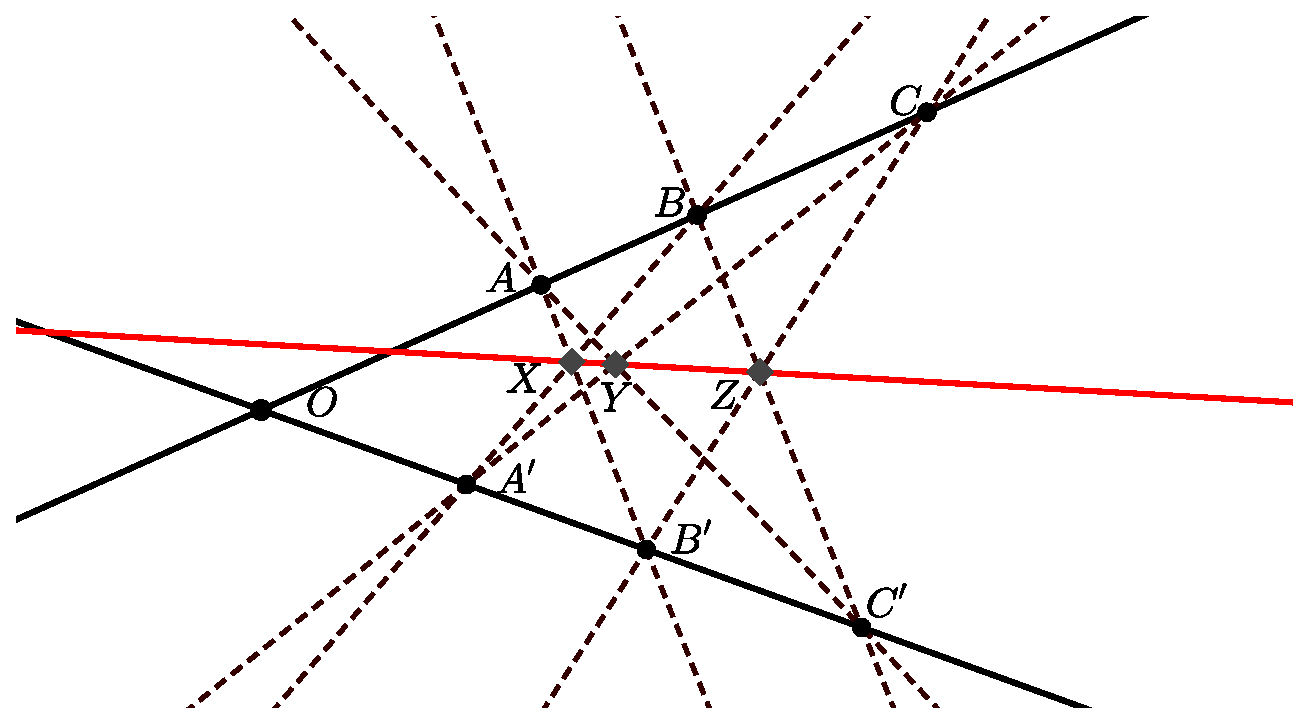
\includegraphics[scale=.5]{Graficos/Pappus.eps}
		\caption{Ilustración del Teorema de Pappus.}
		\label{C3_pappus}
	\end{figure}
\end{theo}
\begin{proof}
	Dado que en el plano proyectivo las rectas son hiperplanos, y haciendo uso del corolario~\ref{C1_cor_rectaHiperplano}, las rectas $r$ y $r'$ se cortan en un punto $O$. 
	
	Si alguno de los seis puntos es $O$, el teorema es trivial ya que dos de los puntos $X,Y$ y $Z$ coincidirían, con lo que tendríamos dos puntos trivialmente alineados. Trataremos pues el caso en que todos ellos son diferentes de $O$.
	
	La demostración consistirá en hallar las coordenadas de los puntos $X,Y,Z$ y comprobar que están alineados. Para ello es necesario establecer una referencia proyectiva. Por comodidad elegimos
	\begin{equation*}
		\mf{R}=\{A,B,C';B'\}
	\end{equation*}
	Comprobemos que es referencia. Por hipótesis, dado que son distintos, los puntos $A,B$ y $C'$ forman un triángulo no degenerado. Por tanto, para ver que cada $3$ de ellos son proyectivamente independientes, bastaría comprobar que el punto $B'$ no está en ninguno de los lados del triángulo $ABC'$.
	
	Dado que $B'\in r'\smz$ es claro que no pertenece a la recta $AB=r$. Tampoco está en $AC'$ ya que, en caso contrario, $B'\in r'\cap AC'=\{C'\}$, lo cual es absurdo pues los puntos $B'$ y $C'$ son distintos. Por último, no pertenece a $BC'$, pues en caso contrario de nuevo tendríamos que $B'\in r'\cap BC'=\{C'\}$. 
	
	Una vez demostrado que $\mf{R}$ es una referencia proyectiva, las coordenadas de los puntos $A,B,C'$ y $B'$ respecto a dicha referencia son
	\begin{equation*}
		A=(1:0:0) \ ; \qquad B=(0:1:0) \ ; \qquad C'=(0:0:1) \ ; \qquad B'=(1:1:1)
	\end{equation*}
	Estamos en situación de hallar las coordenadas de los puntos $X,Y$ y $Z$ respecto a la referencia $\mf{R}$. Realizaremos el mismo procedimiento para todos los puntos: hallaremos las ecuaciones, paramétricas o implícitas, de las rectas cuya intersección es el punto en cuestión, y a partir de ellas calcularemos posteriormente dicha intersección.
	\begin{itemize}
		\item Punto $X=AB'\cap A'B$.
		
		Dado que las coordenadas respecto a nuestra referencia de los puntos $A$ y $B'$ son conocidas, la ecuación implícita de la recta $AB'$ es
		\begin{equation*}
			\left| \begin{array}{ccc}
				x & y & z\\
				1 & 0 & 0\\
				1 & 1 & 1
			\end{array}\right| =0 \ \sii \ z-y=0
		\end{equation*}
		Para la recta $ A'B$ primero debemos hallar las coordenadas de $A'$ respecto de $\mf{R}$. Es un punto de $B'C'=r'$ distinto de $O,B',C'$. Las ecuaciones paramétricas de $B'C'$, tomando como representantes los vectores $(1,1,1)$ y $(0,0,1)$, son
		\begin{equation}
			\label{C3_papus_eqparam_r}
			r'=B'C':=\{[\lambda(1,1,1)+\mu(0,0,1)]\tq \lambda,\mu\in E\}=\{(\lambda:\lambda:\mu+\lambda)\tq \lambda,\mu\in E\}
		\end{equation}
		Por lo que $A'$ es un punto de la forma $(\lambda:\lambda:\mu+\lambda)$. Dado que no es el punto $C'$, $\lambda\not=0$, pudiendo así dividir por $\lambda$. Queda
		\begin{equation*}
			A'=(1:1:1+\frac{\mu}{\lambda})=(1:1:\theta)\tq \theta=1+\frac{\mu}{\lambda}
		\end{equation*}
		Tengamos en cuenta que como $A'\not=B'$, $\theta\not=1$. Además, $A'\not=O$ por lo que nos falta una restricción para $\theta$. Calculamos el punto $O$ para hallarla. La ecuación implícita de $r=AB$ es 
		\begin{equation*}
			\left| \begin{array}{ccc}
				x & y & z\\
				1 & 0 & 0\\
				0 & 1 & 0
			\end{array}\right| =0 \ \sii \ z=0
		\end{equation*}
		Con ello se obtiene que el punto de corte cumple $\mu=-\lambda$. Por tanto, la intersección de ambas rectas es el punto $(\lambda:\lambda:0)=(1:1:0)$. La restricción que debemos imponer a $\theta$ para que $A'\not=O$ es que $\theta\not=0$. Así
		\begin{equation*}
			A'=(1:1:\theta)\tq \theta=1+\frac{\mu}{\lambda}, \theta\not=0, \theta\not=1
		\end{equation*}
		La ecuación implícita de la recta $A'B$ es
		\begin{equation*}
			\left| \begin{array}{ccc}
				x & y & z\\
				1 & 1 & \theta\\
				0 & 1 & 0
			\end{array}\right| =0 \ \sii \ \theta x+z=0
		\end{equation*}
		Finalmente resolviendo el sistema 
		\begin{equation}
			\begin{split}
				AB':&z-y=0\\
				A'B:&\theta x+z=0
			\end{split}
		\end{equation}
		obtenemos el punto $X=AB'\cap A'B$
		\begin{equation}
			\label{C3_pappus_X}
			X=(1:\theta:\theta)
		\end{equation}
		
		\item Punto $Z=BC'\cap B'C$.
		
		La ecuación implícita de la recta $BC'$ es
		\begin{equation*}
			\left| \begin{array}{ccc}
				x & y & z\\
				0 & 1 & 0\\
				0 & 0 & 1
			\end{array}\right| =0 \ \sii \ x=0
		\end{equation*}
		Para describir la recta $B'C$ debemos hallar antes el punto $C$. Este se encuentra en la recta $AB$, que descrita a través de las ecuaciones paramétricas es
		\begin{equation*}
			AB:=\{[\alpha(1,0,0)+\beta(0,1,0)]\tq \alpha,\beta\in E\}=\{(\alpha:\beta:0)\tq \alpha,\beta\in E\}
		\end{equation*}
		Dado que $C\not=B$, se tiene que $\alpha\not=0$, por lo que podemos dividir por ella
		\begin{equation*}
			C=(1:\frac{\beta}{\alpha}:0)=(1:\mu:0)\tq \mu=\frac{\beta}{\alpha}
		\end{equation*}
		Por otro lado $C\not=O=(1:1:0)$, lo cual implica que $\mu\not=1$. Además $C\not=A$, por lo que $\mu\not=0$. Así, finalmente el punto $C$ es
		\begin{equation*}
			C=(1:\mu:0)\tq \mu=\frac{\beta}{\alpha},\mu\not=0,\mu\not=1
		\end{equation*}
		Ahora ya podemos calcular las ecuaciones paramétricas de la recta $B'C$, las cuales, en coordenadas no homogéneas, vienen dadas por
		\begin{equation*}
			B'C:=\{[(1,\mu,0)+\nu(1,1,1)]\tq \nu\in\overline{\K}\}=\{(1+\nu:\mu+\nu:\nu)\tq \nu\in\overline{\K}\}
		\end{equation*}
		El punto de intersección de las rectas $BC'$ y $B'C$ cumple $1+\nu=0$. Por tanto, $\nu=-1$ y la intersección de ambas es 
		\begin{equation}
			\label{C3_pappus_Z}
			Z=(0:\mu-1:-1)
		\end{equation}
		
		
		\item Punto $Y=AC'\cap A'C$.
		
		La ecuación implícita de la recta $AC'$ es
		\begin{equation*}
			\left| \begin{array}{ccc}
				x & y & z\\
				1 & 0 & 0\\
				0 & 0 & 1
			\end{array}\right| =0 \ \sii \ y=0
		\end{equation*}
		Por otro lado, las ecuaciones paramétricas de $A'C$, teniendo en cuenta las restricciones antes impuestas a $\theta$ y $\mu$, son
		\begin{equation*}
			A'C:=\{[(1,1,\theta)+\xi(1,\mu,0)]\tq \xi\in\overline{\K}\}=\{(1+\xi:1+\mu\xi:\theta)\tq \xi\in\overline{\K}\}
		\end{equation*}
		El punto de intersección de ambas rectas cumple $1+\mu\xi=0$, con lo cual $\xi=\frac{-1}{\mu}$. Finalmente el punto $Y$ es
		\begin{equation}
			\label{C3_pappus_Y}
			Y=(1-\frac{1}{\mu}:0:\theta)=(\mu-1:0:\mu\theta)
		\end{equation}
		
	\end{itemize}
	Una vez que tenemos las coordenadas de los tres puntos respecto a la referencia $\mf{R}$ falta comprobar que están alineados. Para ello, sus representantes deben ser coplanarios, es decir, su determinante debe ser nulo. Haciendo uso de las ecuaciones~\eqref{C3_pappus_X},~\eqref{C3_pappus_Y} y~\eqref{C3_pappus_Z} comprobamos que esto se cumple
	\begin{equation*}
		\left| \begin{array}{ccc}
			1 & \mu-1 & 0\\
			\theta & 0 & \mu-1\\
			\theta & \mu\theta & -1
		\end{array}\right| =(\mu-1)^2\theta-(\mu-1)\mu\theta+(\mu-1)\theta=\mu^2\theta+\theta-2\mu\theta-\mu^2\theta+2\mu\theta-\theta=0
	\end{equation*}
	Es importante observar que en general el determinante de los representantes de tres puntos proyectivos no está bien definido, debido a que podemos coger múltiplos. Sin embargo en este caso, al ser igual a cero, sí lo está. Por ello, el teorema queda demostrado.
\end{proof}
Recordemos que gracias al principio de dualidad, dado un teorema, automáticamente su dual es cierto. Así, podemos enunciar el Teorema de Pappus para el plano proyectivo dual y quedará demostrado, por el simple hecho de haber demostrado el teorema en el plano proyectivo.
\begin{theo}[Teorema de Pappus Dual]
	Sea $\proy(E^*)=\proy^*$ un plano proyectivo dual y sean $R$ y $R'$ dos puntos distintos de $\proy^*$. Entonces, para cualesquiera seis rectas distintas $a,b,c,a',b',c'$ tales que $R\in a,b,c$ y $R'\in a',b',c'$; las rectas
	\begin{equation*}
		\engen{a\cap b',a'\cap b} \ ; \qquad \engen{a\cap c',a'\cap c} \ ; \qquad \engen{b\cap c',b'\cap c}
	\end{equation*}
	son concurrentes.
\end{theo}
\begin{proof}
	Trivial por dualidad.
\end{proof}
\begin{figure}[h]
	\centering
	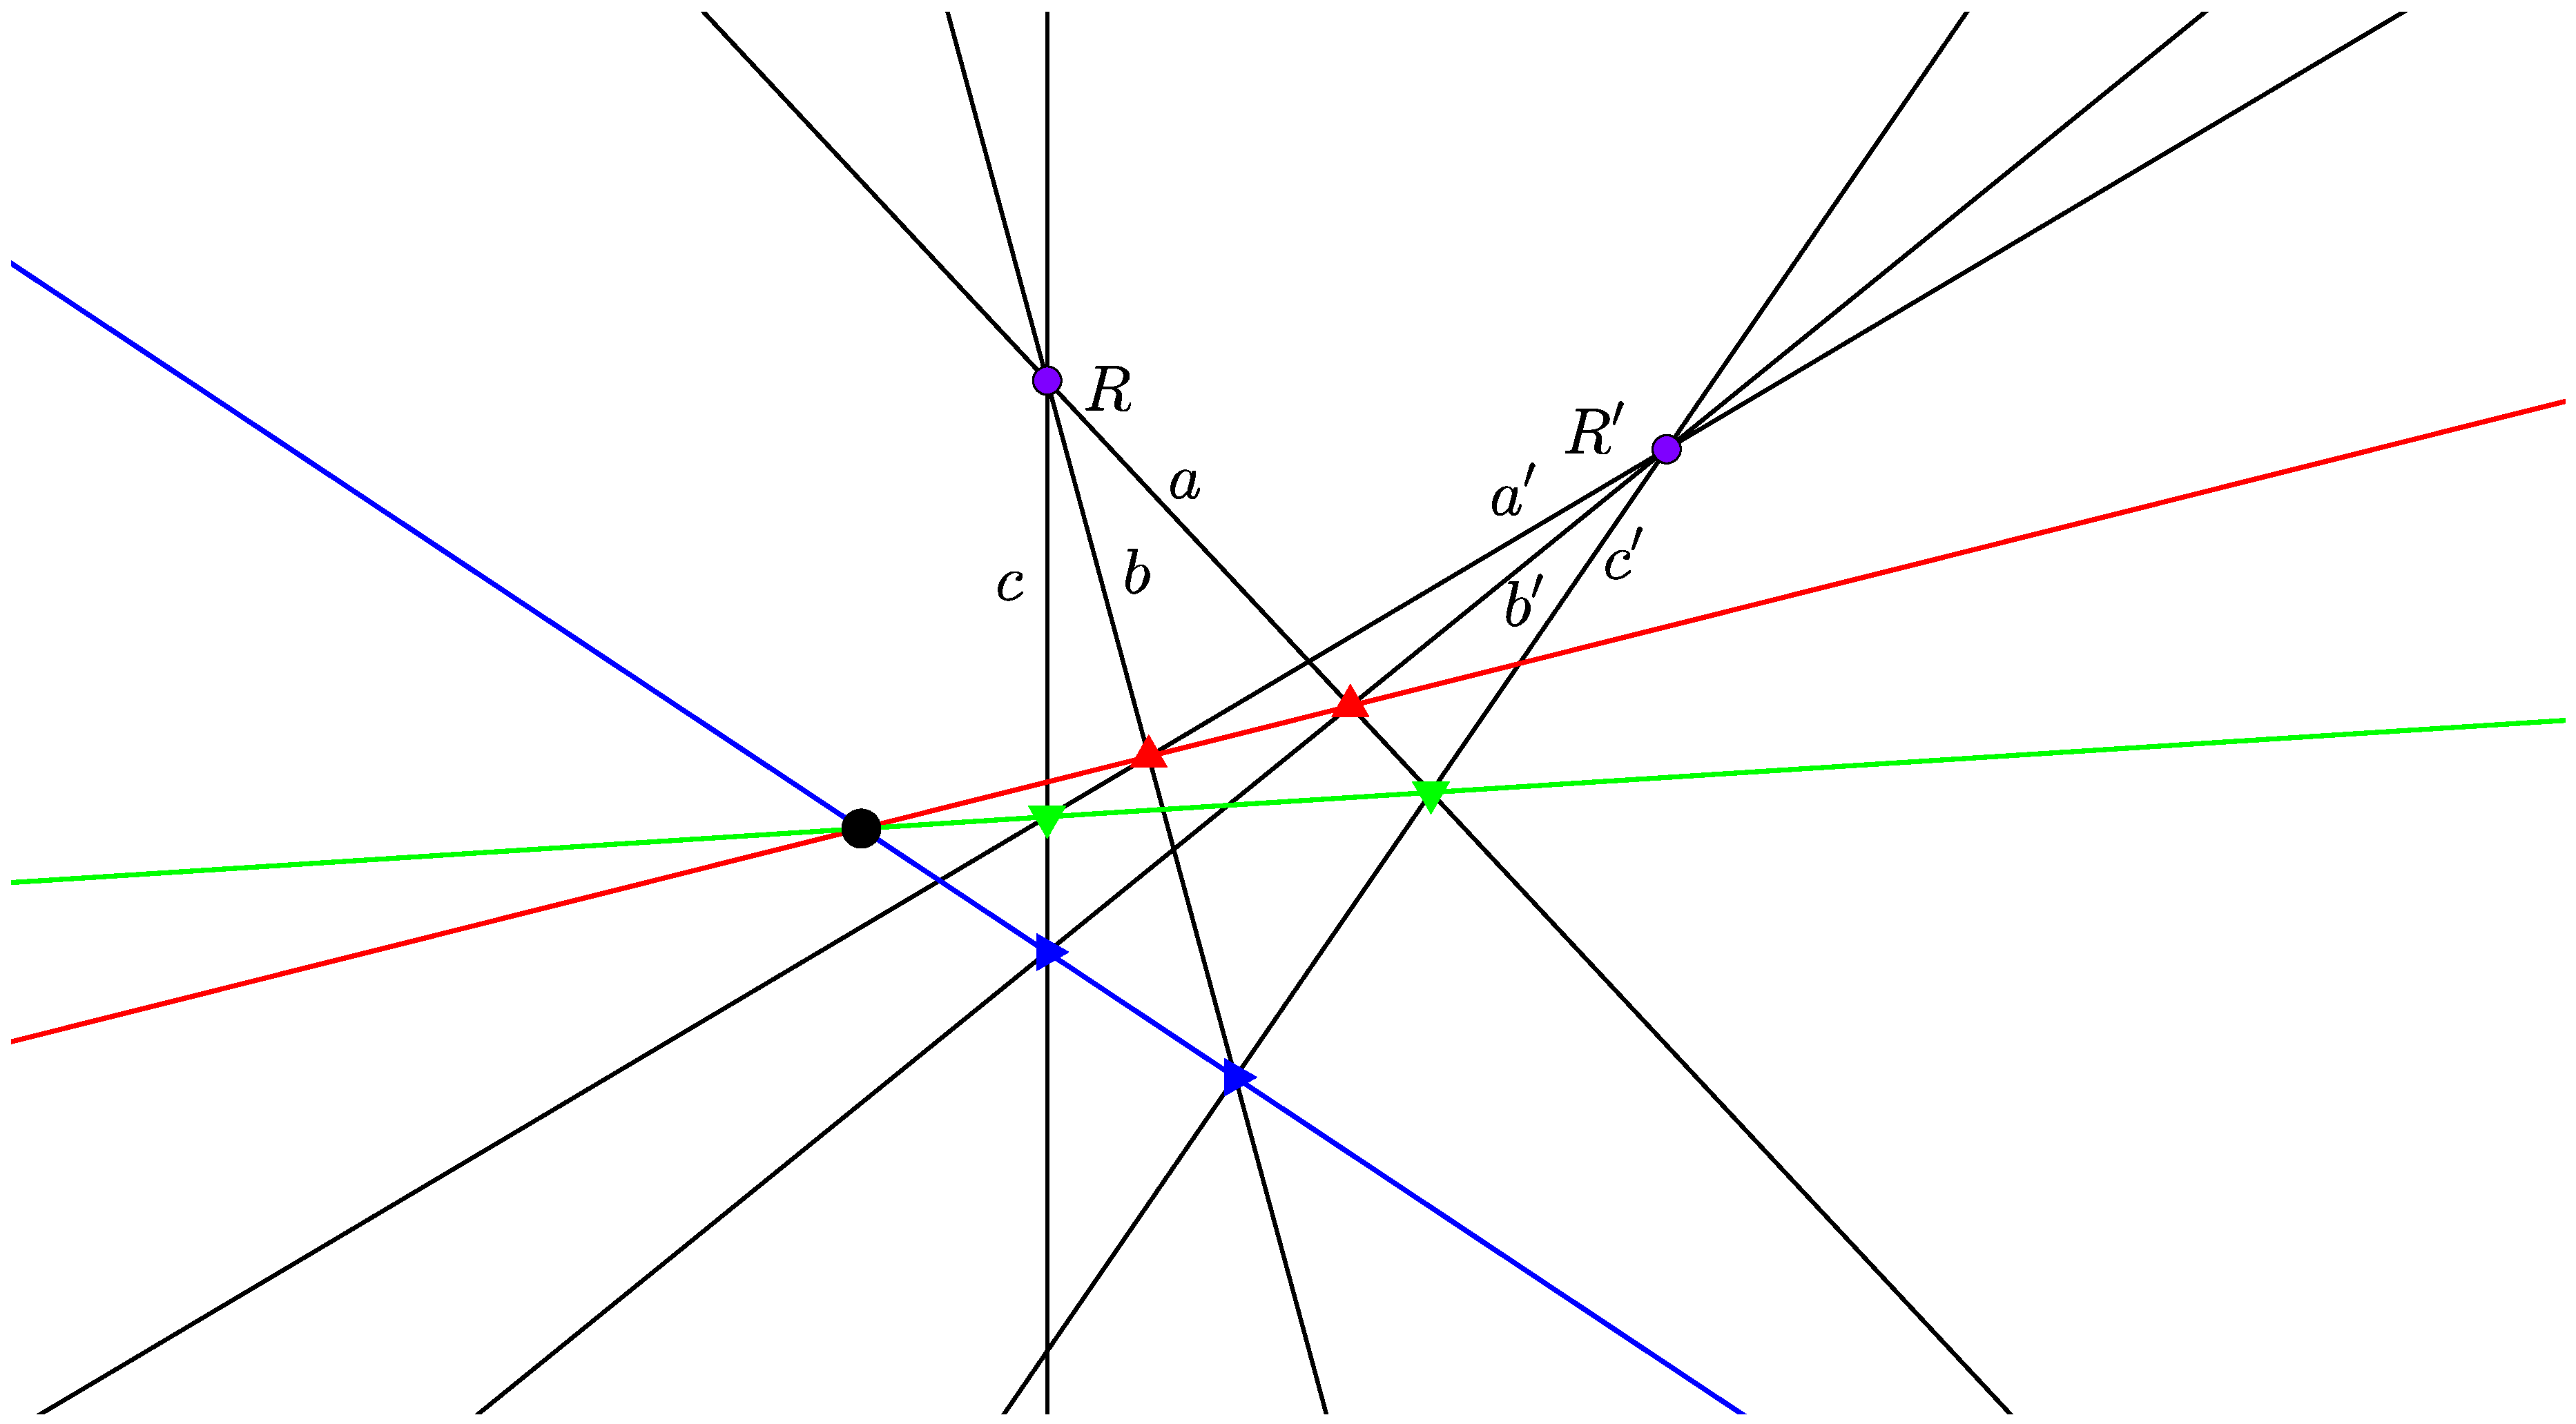
\includegraphics[scale=.2]{Graficos/Dual_Teorema_de_Papus.eps}
	\caption{Ilustración del Teorema de Pappus Dual.}
	\label{C3_pappusDual}
\end{figure}

	\chapter{Aplicaciones Proyectivas}
\label{C4}
En este capítulo vamos a tratar de extrapolar uno de los conceptos más centrales del álgebra lineal al contexto proyectivo. Tratamos de estudiar las aplicaciones entre espacios proyectivos cuyo comportamiento consideramos ``bueno''.

En el mundo lineal, estas aplicaciones eran los llamados homomorfismos entre espacios vectoriales o símplemente aplicaciones lineales. Aquí, en el mundo de los rayos, las llamaremos \ti{aplicaciones proyectivas}.
\section{Definición}
\label{C4_definicion}
Sean dos espacios proyectivos $X$ e $Y$ asociados a sendos espacios vectoriales, $\widehat{X}$ e $\widehat{Y}$ respectivamente.

Nuestro objetivo es definir una aplicación proyectiva entre dos espacios proyectivos a partir de una aplicación lineal entre sus respectivos espacios lineales de forma natural. Intentémoslo y veamos qué dificultades se nos presentan.

Sea $\widehat{h}:\widehat{X}\to\widehat{Y}$ una aplicación lineal arbitraria. Lo deseable sería definir la aplicación proyectiva asociada a $\widehat{h}$ como aquella que, a cadaa rayo le asigna el rayo engendrado por la imagen de uno de sus representantes. Visto formalmente, si $x=\class{u}$:
\[\begin{array}{c}
X\stackrel{h}{\to}Y\\
x\mapsto\class{\widehat{h}(u)}
\end{array}\]
Este intento de definición tan intuitivo e inocente presenta dos problemas. El primero de ellos es que si $\widehat{h}(u)=0$ entonces el rayo $\class{\widehat{h}(u)}$ no está definido.

Esto lo arreglamos de una forma natural, restringiendo el dominio de $\widehat{h}$ a los vectores de $\widehat{X}$ que no se anulan mediante $\widehat{h}$. Es decir, ahora $\widehat{h}$ queda definida en $\widehat{X}\setminus \ker\left(\widehat{h}\right)$.

Trasladando esta restricción al contexto proyectivo obtenemos este segundo intento de definición de aplicación proyectiva asociada a cierta aplicación lineal:
\[\begin{array}{c}
X\setminus\proy\left(\ker\left(\widehat{h}\right)\right)\stackrel{h}{\to}Y\\
x\mapsto\class{\widehat{h}(u)}
\end{array}\]
Antes de hacer algunas aclaraciones adicionales acerca de este primer problema que se nos ha presentado, demos una pequeña definición (por comodidad tipográfica).
\begin{defi}[Centro]
	\label{C4_def_centro}
	Se denomina \ti{centro} de una aplicación $\widehat{h}$ entre dos espacios lineales $\widehat{X}$ e $\widehat{Y}$ a la variedad proyectiva:
	\[\mc{Z}:\equals{not.}\proy\left(\ker\left(\widehat{h}\right)\right)\]
\end{defi}
Tras este breve inciso sobre la notación, veamos que, en efecto, hemos resuelto el problema que se nos planteaba, es decir, hemos eliminado del dominio todos los rayos que no tenían imagen definida. Si hubiera algún rayo con imagen no definida, alguno de sus representantes debería pertenecer al núcleo de $\widehat{h}$ (y por tanto todos). Pero esto no es posible ya que el rayo engendrado por este representante estaría en el centro de $h$.

El segundo problema que planteaba nuestra definición era saber si está bien definida. En efecto, siempre que definamos una aplicación y los elementos de nuestro conjunto de salida no tengan una representación única, debemos comprobar que la imagen de la función es independiente del representante escogido. En este caso es un juego de niños:

Sean $\class{u'}=x=\class{u}$. Es evidente que $u' = \lambda u$ para cierto $\lambda$ no nulo. Entonces:
\[\class{\widehat{h}(u')}=\class{\widehat{h}(\lambda u)}=\class{\lambda\widehat{h}(u)}=\class{\widehat{h}(u)}\]

Para terminar la sección advertimos de que en algunos textos, a la hora de representar una aplicación proyectiva omiten (abusando de notación) especificar que al espacio de partida se le extrae el centro $\mc{Z}$. 
\section{Propiedades Elementales}
En esta sección estudiaremos diversas propiedades básicas de las aplicaciones proyectivas. Propiedades tales como el comportamiento de las aplicaciones proyectivas inyectivas y sobreyectivas, la clausura de estas respecto de la composición, cómo estas aplicaciones parametrizan variedades proyectivas y un lema de la correspondencia bastante útil.

POSPUESTO HASTA QUE LO VEAMOS EN CLASE

Un resultado deseable, aunque para nada inmediato, es el de que podamos clasificar a las aplicaciones lineales que inducen cierta aplicación proyectiva por ser múltiplos entre si. Veamoslo:
\begin{theo}[Lema de la Correspondencia]
	\label{C4_teo_lemaCorrespondencia}
	Dos aplicaciones lineales no nulas producen la misma aplicación proyectiva si y solo si son múltiplos la una de la otra.
\end{theo}
\begin{proof}
	\begin{itemize}
		\item[$\bra$] Sean dos aplicaciones lineales $\widehat{g},\widehat{h}:E\to E'$ tales que inducen la misma variedad proyectiva. Esto es:
		\[\begin{array}{c}
		\proy(E)\setminus\mc{Z}\stackrel{\varphi}{\to}\proy(E')\\
		x=\class{u}\mapsto\varphi(x)=\class{\widehat{g}(u)}=\class{\widehat{h}(u)}
		\end{array}\]
		Para que esto pueda suceder es condición indispensable que ambas aplicaciones tengan el mismo kernel:
		\[\mc{Z}=\proy(\ker(\widehat{h}))=\proy(\ker(\widehat{g}))\sii \ker(\widehat{h})=\ker(\widehat{g})\]
		Por ende nuestro objetivo es demostrar que dicho $\lambda_u$ es el mismo para todos los vectores.
		
		Distingamos dos casos (para no talar árboles de más echaremos las cuentas rápido).
		\begin{itemize}
			\item Sean $u,v\in E\setminus\ker(\widehat{g})$ tales que $u=\mu v$. Tenemos que:
			\[
			\widehat{g}(u)=\lambda_u\widehat{h}(u)
			\sii\mu\widehat{g}(v)=\lambda_u\mu\widehat{h}(v)\sii\lambda_v\widehat{h}(v)=\lambda_u\widehat{h}(v)\sii\lambda_u=\lambda_v
			\]
			\item Sea $u,v\in E\setminus\ker(\widehat{g})$ linealmente independientes y sea $w=u+v$. Echando las cuentas:
			\begin{multline}\widehat{g}(w)=\lambda_w\widehat{h}(w)\sii\\\sii\widehat{g}(u)+\widehat{g}(v)=\lambda_w(\widehat{h}(u)+\widehat{h}(v))\sii\\
			\sii \lambda_u\widehat{h}(u)+\lambda_v\widehat{h}(v)=\lambda_w(\widehat{h}(u)+\widehat{h}(v))\sii\\
			(\lambda_u-\lambda_w)\widehat{h}(u)+(\lambda_v-\lambda_w)\widehat{h}(v)=0\end{multline}
			Como $\widehat{h}(u)$ y $\widehat{h}(v)$ son linealmente independientes (compruébese), se tiene que: \[\lambda_u=\lambda_v=\lambda_w\].
		\end{itemize}
		\item[$\bla$] Inmediato, ya que si $\widehat{h}(u)=\lambda\widehat{g}(u)$ para todo $u$, tomando clases:
		\[h(u)=\class{\widehat{h}(u)}=\class{\lambda\widehat{g}(u)}=\class{\widehat{g}(u)}=g(u)\]
		Sabemos que las imágenes de $\widehat{g}$ y $\widehat{h}$ son iguales salvo múltiplos para todos los vectores que no pertenecen al núcleo, con lo que:
		\[\class{\widehat{g}(u)}=\class{\widehat{h}(u)}\ \forall u\not\in\widehat{\mc{Z}}\ra\widehat{g}(u)=\lambda_u\widehat{h}(u)\]
	\end{itemize}
\end{proof}
Al teorema \ref{C4_teo_lemaCorrespondencia} le bautizamos con el nombre de ``lema de la correspondencia'', porque lo que viene a decir (siendo muy retorcidos) es que las aplicaciones proyectivas entre dos espacios proyectivos están en biyección con los elementos del espacio proyectivo $\proy(\mathrm{Hom}(\widehat{X},\widehat{Y}))$.
\section{Homografías}
\section{Proyecciones Cónicas}
Dedicaremos esta sección al estudio de un tipo especialmente relevante de aplicaciones proyectivas no homográficas, las llamadas \ti{proyecciones cónicas}.

Antes de lanzarnos al estudio general de estas aplicaciones presentemos un par de ejemplos que más adelante nos ayudarán a entender intuitivamente el por qué del apellido ``cónicas'' de estas aplicaciones.

\begin{exa}[Punto sobre Recta]
	\label{C4_exa_puntoRecta}
	En el plano proyectivo $\proy^2$ consideramos un punto $z$ y una recta $Y$ (recordemos que es un subespacio proyectivo) tal que $z\not\in Y$. En estas condiciones definimos la aplicación:
	\[\begin{array}{c}
		\proy^2\setminus\{z\}\stackrel{h}{\to} Y\\
		x\mapsto h(x)=\engen{x,z}\cap Y
	\end{array}\]
\end{exa}

No demostraremos que la aplicación del ejemplo \ref{C4_exa_puntoRecta} es, en efecto, una aplicación proyectiva, ya que al final de la sección daremos una demostración general para todas las proyecciones cónicas, de las que esta aplicación en concreto es un caso particular.

El ejemplo \ref{C4_exa_puntoRecta} se puede generalizar para dimensiones superiores, basta mantener que $z$ sea un punto de $\proy^n$ e $Y$ un hiperplano.
\begin{exa}[Punto sobre Hiperplano]
	\label{C4_exa_puntoHiperplano}
	En el plano proyectivo $\proy^n$ consideramos el punto $z$ y el hiperplano $Y$ tal que $z\not\in Y$. Definimos la aplicación:
	\[\begin{array}{c}
	\proy^n\setminus\{z\}\stackrel{h}{\to} Y\\
	x\mapsto h(x)=\engen{x,z}\cap Y
	\end{array}\]
\end{exa}
Otra generalización de los ejemplos anteriores es la siguiente (menos intuitiva y más dificil de ver):
\begin{exa}
	En el espacio proyectivo $\proy^3$ se consideran las rectas $l$ y $l$ tales que $l\cap l'=\emptyset$. Definimos la aplicación:
	\[\begin{array}{c}
	\proy^3\setminus l\stackrel{h}{\to}l'\\
	x\mapsto\engen{x,l}\cap l'
	\end{array}\]
\end{exa}
Observamos simplemente que $\engen{x,l}\cap l'$ siempre se corta con $l$ en un punto (consecuencia inmediata de la fórmula de Grassmann).

Llegados a este punto, ha llegado la hora de definir \ti{proyección cónica} en toda su generalidad.
\begin{defi}[Proyección Cónica]
	\label{C4_def_proyeccionConica}
	Sean $X$ un espacio proyectivo y $Z$ e $Y$ dos variedades proyectivas de $X$ tales que:
	\begin{enumerate}
		\item $Z\cap Y=\emptyset$
		\item $\dim(Z)+\dim(Y)=\dim(X)-1$
	\end{enumerate}
	Definimos la aplicación:
	\[\begin{array}{c}
	X\setminus Z\stackrel{h}{\to} Y\\
	x\mapsto\engen{x,Z}\cap Y
	\end{array}\]
\end{defi}
Automáticamente se nos presentan una serie de cuestiones que trataremos de responder a continuación:
\begin{enumerate}
	\item ¿La intersección $\engen{x,Z}\cap Y$ es siempre un único punto?
	\item ¿$h$ es una aplicación proyectiva? ¿Cuál es su aplicación lineal asociada?
\end{enumerate}
Como diría Jack el Destripador, vayamos por partes:
\begin{prop}[Intersección Unipuntual]
	\label{C4_prop_interseccionUnipuntual}
	En las condiciones de la definición \ref{C4_def_proyeccionConica} la intersección $\engen{x,Z}\cap Y$ tiene dimensión nula. Es decir, es un punto proyectivo.
\end{prop}
\begin{proof}
	Usando la fórmula de Grassmann:
	\begin{equation}
		\label{C4_eq_interseccionUnipuntual1}
		\dim\engen{\engen{x,Z},Y}=\dim\engen{x,Z}+\dim\engen{Y}-\dim\engen{x,Z}\cap Y
	\end{equation}
	En primer lugar, veamos cuál es la dimensión de $\engen{x,Z}$, para lo cual usaremos, de nuevo, la fórmula de Grassmann.
	\begin{equation}
		\label{C4_eq_interseccionUnipuntual2}
		\dim\engen{x,Z}=\dim(x)+\dim(Z)+\dim(x\cap Z)
	\end{equation}
	Como $\dim(x)=0$ (por ser un punto) y la dimensión de $\dim(x\cap Z)=-1$, ya que, por definición de proyección cónica $x\not\in Z$, y por tanto $x\cap Z=\emptyset$. Sustituyendo en \eqref{C4_eq_interseccionUnipuntual2} se obtiene:
	\begin{equation}
		\label{C4_eq_interseccionUnipuntual3}
		\dim\engen{x,Z}=\dim(Z)+1
	\end{equation}
	Sustituyendo este resultado en \eqref{C4_eq_interseccionUnipuntual1} obtenemos:
	\begin{equation}
		\label{C4_eq_interseccionUnipuntual4}
		\dim\engen{\engen{x,Z},Y}=\dim(Z)+1+\dim\engen{Y}-\dim\engen{x,Z}\cap Y
	\end{equation}
	Como, por hipótesis $\dim(Z)+\dim(Y)=\dim(X)-1$, sustituyendo en \eqref{C4_eq_interseccionUnipuntual4} queda:
	\begin{equation}
		\label{C4_eq_interseccionUnipuntual5}
		\dim\engen{\engen{x,Z},Y}=\dim(X)-\dim\engen{x,Z}\cap Y
	\end{equation}
	Centrémonos ahora en el otro miembro de la igualdad. En primer lugar, es claro que:
	\[\dim\engen{\engen{x,Z},Y}=\dim\engen{x,Z,Y}\]
	Parece intuitivo pensar que $Z$ e $Y$ generan $X$. Veámoslo:
	\begin{equation}
		\label{C4_eq_interseccionUnipuntual6}
		\dim\engen{Z,Y}=\dim(Z)+\dim(Y)-\dim(Z\cap Y)
	\end{equation}
	Como, por hipótesis, $Z\cap Y$ es el vacío, y, además, la suma de las dimensiones de $Z$ e $Y$ dan la dimensión de $X$ menos $1$, nos queda que, efectivamente:
	\begin{equation}
		\label{C4_eq_interseccionUnipuntual7}
		\dim\engen{Z,Y}=\dim(X)
	\end{equation}
	Por ende, $\dim\engen{Z,Y,x}=\dim(X)$, y, podemos sustituir en \eqref{C4_eq_interseccionUnipuntual5}:
	\begin{equation}
		\label{C4_eq_interseccionUnipuntual8}
		\dim(X)=\dim(X)-\dim\engen{x,Z}\cap Y
	\end{equation}
	Despejando, el resultado se sigue inmediatamente.
\end{proof}
La proposición \ref{C4_prop_interseccionUnipuntual} prueba que $h$ está bien definida como aplicación.

Una pequeña observación antes de probar que las proyecciones cónicas son, efectivamente, aplicaciones proyectivas, es que los espacios lineales asociados a $Z$ y a $Y$ son complementarios.
\begin{obs}[Espacios Lineales Complementarios]
	\label{C4_obs_espaciosComplementarios}
	Como la intersección de las variades proyectivas $Z$ e $Y$ es el vacío, esta intersección tiene dimensión $-1$. Por ende, el espacio lineal asociado a esta intersección es el nulo. Es decir:
	\[Z\cap Y=\emptyset\sii\widehat{Z}\cap\widehat{Y}=\zset\]
	Además, la suma de las dimensiones de $Z$ e $Y$ es la dimensión de $X$ menos $1$. Usando esto:
	\begin{multline*}
		\dim(Y)+\dim(Z)=\dim(X)-1\sii\\
		\sii \dim(\widehat{Y})-1+\dim(\widehat{Z})-1=\dim(\widehat{X})-1-1\sii\\
		\sii \dim(\widehat{Y})+\dim(\widehat{Z})-2=\dim(\widehat{X})-2\sii\\
		\sii \dim(\widehat{Y})+\dim(\widehat{Z})=\dim(\widehat{X})
	\end{multline*}
	En su conjunto, esto quiere decir que se tiene la siguiente descomposición en suma directa del espacio lineal:
	\[\widehat{X}=\widehat{Y}\oplus\widehat{Z}\]
\end{obs}
Probemos ahora que las proyecciones cónicas son aplicaciones proyectivas. Y que, de hecho, son las aplicaciones proyectivas asociadas a \ti{proyecciones vectoriales}. (De ahí surge el nombre de ``proyección'').
\begin{prop}[Proyección Vectorial]
	\label{C4_prop_proyeccionVectorial}
	La aplicación $h$ tiene a la siguiente aplicación lineal (proyección vectorial de $\widehat{X}$ sobre $\widehat{Y}$) como asociada:
	\[\begin{array}{c}
	\widehat{X}=\widehat{Z}\oplus\widehat{Y}\stackrel{\widehat{h}}{\to}\widehat{Y}\\
	u=v+w\mapsto w
	\end{array}\]
	Siendo $v\in \widehat{Z}$ y $w\in \widehat{Y}$, es decir, la descomposición de $x$ en suma de vectores de $\widehat{Z}$ y $\widehat{Y}$.
\end{prop}
\begin{proof}
	Comprobar que $\widehat{h}$ es una aplicación lineal con núcleo $\widehat{Z}$ es inmediato y se deja al lector. Hecho esto, suponiendo que $x=\class{u}$, basta ver que $h(x)=\class{\widehat{h}(u)}$ para cualquier $x\in X$.
	
	\[\class{\widehat{h}(u)}=\class{\widehat{h}(v+w)}=\class{w}\]
	
	Veamos que $\class{w}\in \engen{x,Z}\cap Y$, demostrando así lo que queríamos.
	
	En primer lugar, sabemos que $w$ no es el vector nulo, ya que si lo fuera, el rayo $x$ estaría en el centro. Dicho esto, como $Y=\proy(\widehat{Y})$, y como $w\in\widehat{Y}$, entonces $\class{w}\in Y$.
	
	Para demostrar que $\class{w}\in\engen{x,Z}$ basta con darse cuenta de que $\engen{x,Z}=\proy({\lengen{u,\widehat{Z}}})$. Como $u = v+w$ se tiene que $w=u-v\in\lengen{u, \widehat{Z}}$, luego, tomando clases: \[\class{w}=\class{u-v}\in\proy(\lengen{u,\widehat{Z}})=\engen{x,Z}\]
\end{proof}
La proposición \ref*{C4_prop_proyeccionVectorial} demuestra que las proyecciones cónicas en general son aplicaciones proyectivas, dando la aplicación lineal asociada (una proyección vectorial).

Antes de finalizar la sección daremos una explicación del por qué del apellido ``cónicas'' de estas aplicaciones. Además, daremos dos ejemplos detallados para que el lector se familiarice con el tratamiento de estas aplicaciones, y que, además, constituye un gran repaso de capítulos anteriores. Por último propondremos un ejercicio al lector.

\begin{obs}[Cónicas]
	\label{C4_obs_conicas}
	Este apellido es debido a que, en el caso particular presentado en el ejemplo \ref{C4_exa_puntoHiperplano}, si tomamos la imagen de una circunferencia por la proyección cónica obtenemos una curva cónica. Esta curva es la formada por la intersección entre el hiperplano $Y$ la familia de rectas que pasan por $z$ y un punto de la circunferencia.
\end{obs}
\begin{exa}[Proyección Punto -- Plano Degenerada]
	Dado el punto $z$ y el plano $\pi$, se pide hallar la imagen de un punto genérico $p$ por la proyección cónica con centro $z$ sobre $\pi$.
	(POR HACER)
\end{exa}

\begin{exa}[Proyección Punto -- Plano]
	Dado el punto $z$ y el plano $\pi$, se pide hallar la imagen de un punto genérico $p$ por la proyección cónica con centro $z$ sobre $\pi$.
	(POR HACER)
\end{exa}

\begin{prob}
	Enumere las proyecciones cónicas de $\proy^4$, clasificándolas en función de las subvariedades $Z$ e $Y$ que las caracterizan.
\end{prob}
\section{Teorema de Desargues}
	\chapter{Razón Doble}
El objetivo de este capítulo es ver que, dadas dos rectas proyectivas $\proy(E)$ y $\proy(E')$, existe una homografía que transforma cuatro puntos distintos cualesquiera de $\proy(E)$ en otros cuatro puntos distintos de $\proy(E')$. Esto nos llevará a la definición de razón doble y a estudiar sus características y propiedades.

\section{Definición}
Empecemos tratando un caso más sencillo, tres puntos. Es fácil demostrar haciendo uso del álgebra lineal, como haremos a continuación, que, dadas dos rectas proyectivas, existe una única homografía que transforma tres puntos distintos cualesquiera en otros tres puntos distintos.

\begin{prop}
	\label{C5_prop_homografia3puntos}
	Dadas dos rectas proyectivas, $\proy(E)$ y $\proy(E')$, y dadas dos ternas diferentes siempre existe una única homografía que transforma la una en la otra.
\end{prop}
\begin{proof}
	Sean $\{p_0,p_1,p_2\}$ tres puntos distintos de $\proy(E)$. Al ser diferentes podemos tomar dicha terna como referencia proyectiva $\mf{R}$ de $\proy(E)$. Esto nos proporcionará una base de $E$, la correspondiente base asociada $\mc{B}$ a la referencia $\mf{R}$. Sea la terna de puntos distintos $\{p'_0,p'_1,p'_2\}$ de la recta proyectiva $\proy(E')$, podemos hacer lo mismo. Con ello obtenemos una base $\mc{B'}$ de $E'$. 
	
	Existe un único isomorfismo 
	\[\widehat{h}:E\rightarrow E'\]
	que trasforma $\mc{B}$ en $\mc{B'}$. La aplicación proyectiva asociada a esta aplicación lineal es una homografía, de hecho es biyectiva (Corolario~\ref{C4_cor_biyectividad}) que transforma $p_i$ en $p'_i$, para $i=0,1,2$. Además es única al serlo $\widehat{h}$.
\end{proof}

\begin{obs}
	La demostración de la proposición anterior nos permite deducir que dadas dos referencias proyectivas $\mf{R}$ y $\mf{R'}$ de dos rectas proyectivas, existe una única homografía que transforma $\mf{R}$ en $\mf{R'}$.
\end{obs}
Veamos un ejemplo. Para ello recordemos primero que una homografía de la recta proyectiva en sí misma, tomando la misma referencia,  puede definirse a través de coordenadas no homogéneas como
\begin{equation}
	\label{C5_eq_homografia_nohom}
	\frac{x'}{y'}=\theta'=\frac{a\frac{x}{y}+b}{c\frac{x}{y}+d}=\frac{a\theta+b}{c\theta +d}, \ \text{ tal que } ad-bc\not=0
\end{equation}
lo que denominábamos \ti{transformación de Möbius}.
\begin{exa}
	Encontrar la homografía 
	\[h:\proy^1\rightarrow \proy^1\] 
	que trasforma los puntos $\{(0:1),(1:0),(2:1)\}$ en los puntos $\{(1:1),(-1:1),(0:1)\}$.\\
	
	Podemos resolver este ejercicio de varias formas. La primera consistiría en plantear las ecuaciones con la matriz A asociada
	\begin{equation*}
		A\left( \begin{array}{c}
			x\\ y
		\end{array}\right)
		=\left( \begin{array}{cc}
			a&b\\ c&d
		\end{array}\right) 
		\left( \begin{array}{c}
			x\\ y
		\end{array}\right)=\rho
		\left( \begin{array}{c}
		x'\\ y'
	\end{array}\right)
	\end{equation*}
	y, sustituyendo los valores de los puntos dados, resolver el sistema de ecuaciones:
	\begin{equation*}
		\left( \begin{array}{cc}
			a&b\\ c&d
		\end{array}\right) 
		\left( \begin{array}{c}
			0\\ 1
		\end{array}\right)=\rho_1
		\left( \begin{array}{c}
			1\\ 1
		\end{array}\right)
	\end{equation*}
	\begin{equation*}
		\left( \begin{array}{cc}
			a&b\\ c&d
		\end{array}\right) 
		\left( \begin{array}{c}
			1\\ 0
		\end{array}\right)=\rho_2
		\left( \begin{array}{c}
			-1\\ 1
		\end{array}\right)
	\end{equation*}
	\begin{equation*}
		\left( \begin{array}{cc}
			a&b\\ c&d
		\end{array}\right) 
		\left( \begin{array}{c}
			2\\ 1
		\end{array}\right)=\rho_3
		\left( \begin{array}{c}
			0\\ 1
		\end{array}\right)
	\end{equation*}
	Sin embargo, esto puede resultar muy pesado. Si utilizamos la definición de homografía dada por la ecuación~\eqref{C5_eq_homografia_nohom}, el cálculo resulta mucho más llevadero. Así, para determinar la homografía basta hallar la expresión en coordenadas no homogéneas que la define, que se obtiene sustituyendo los valores proporcionados en la ecuación~\eqref{C5_eq_homografia_nohom} y resolviendo el sistema. Observamos que el punto $(1:0)$ se transforma en $\theta=\infty$. Para resolver esta indeterminación, se multiplica la fracción arriba y abajo por $y$
	\begin{equation}
		\theta'=\frac{a\frac{x}{y}+b}{c\frac{x}{y}+d}=\frac{ax+by}{cx +dy}
	\end{equation}
	Así, las ecuaciones resultantes son
	\begin{equation*}
		\begin{split}
			1&=\frac{a0+b1}{c0 +d1}=\frac{b}{d}\ra b=d\\
			-1&=\frac{a1+b0}{c1 +d0}=\frac{a}{c}\ra a=-c\\
			0&=\frac{a2+b1}{c2 +d1}\ra 2a+b=0
		\end{split}
	\end{equation*}
	Observamos que este sistema homogéneo es compatible indeterminado, no nos proporciona valores concretos de los coeficientes de la matriz, sino que dependen de un parámetro. En geometría proyectiva, esto es suficiente para resolver el sistema debido a que, en este caso, nos vale tanto la matriz de la aplicación lineal como un múltiplo suyo. Es decir, nos valen tanto las soluciones del sistema como un múltiplo suyo, \tb{rayos de soluciones}.
	
	Así, para el caso que nos ocupa, $a=\lambda$ y con ello $c=-\lambda, \ b=-2\lambda$ y $d=-2\lambda$, siendo así la matriz
	\begin{equation*}
	 \lambda \left( \begin{array}{cc}
	 1&-2\\ -1&-2
	 \end{array}\right) 
	\end{equation*}
	y podemos tomar sin ningún problema $\lambda=-1$.
	
	Por lo que, tomando $a=-1$, la homografía pedida viene dada por
	\begin{equation*}
		\theta'=\frac{2-\theta}{2+\theta}
	\end{equation*}
	Nótese que no es necesario tener tanto cuidado con $\theta=\infty$, como ya se explicó en el capítulo anterior. Si tenemos en cuenta que $\infty+b=\infty$ y que $\frac{\infty}{\infty}=1$, el resultado es el mismo
	\begin{equation*}
		\theta'=-1=\frac{a\theta+b}{c\theta +d}=\frac{a\infty+b}{c\infty +d}=\frac{a\infty}{c\infty}=\frac{a}{c}\ra a=-c
	\end{equation*}
\end{exa}
\begin{obs}
	De lo explicado en el ejemplo anterior acerca de los sistemas que se obtienen al trabajar con coordenadas no homogéneas se deduce que, para determinar una homografía de $\proy^1$, son suficientes $3$ puntos y sus imágenes, pues nos vale con obtener un rayo de soluciones.
\end{obs}
Encontrar una homografía de una recta proyectiva que lleve cuatro puntos distintos cualesquiera en otros cuatro no es tan sencillo. Para poder caracterizar esta propiedad empezaremos estudiando las características de una homografía que la cumpla.
\begin{lem}
	Sean $\{p_1,p_2,p_3,p_4\}$ y $\{p'_1,p'_2,p'_3,p'_4\}$ ocho puntos distintos de la recta proyectiva $\proy(E)$ respecto a la referencia $\mf{R}$. Sea una homografía
	\[h:\proy(E)\rightarrow \proy(E)\]
	que cumple $h(\theta_i)=\theta'_i$ para todo $i\in\{1,2,3,4\}$, donde $\theta_i$ es el parámetro no homogéneo de $p_i$. Entonces
	\begin{equation}
		\frac{\theta_3-\theta_1}{\theta_3-\theta_2}:\frac{\theta_4-\theta_1}{\theta_4-\theta_2}=\frac{\theta'_3-\theta'_1}{\theta'_3-\theta'_2}:\frac{\theta'_4-\theta'_1}{\theta'_4-\theta'_2}
	\end{equation}
\end{lem}
\begin{proof}
	Dado que $h$ es una homografía de una recta proyectiva en sí misma, y hemos tomado la misma referencia, podemos escribir
	\begin{equation*}
		\theta'=\frac{a\theta+b}{c\theta +d}\tq ad-bc\not=0
	\end{equation*}
	para determinados $a,b,c$ y $d$. Así
	\begin{equation*}
		\frac{\theta'_3-\theta'_1}{\theta'_3-\theta'_2}:\frac{\theta'_4-\theta'_1}{\theta'_4-\theta'_2}=\frac{\frac{a\theta_3+b}{c\theta_3 +d}-\frac{a\theta_1+b}{c\theta_1 +d}}{\frac{a\theta_3+b}{c\theta_3 +d}-\frac{a\theta_2+b}{c\theta_2 +d}}:\frac{\frac{a\theta_4+b}{c\theta_4 +d}-\frac{a\theta_1+b}{c\theta_1 +d}}{\frac{a\theta_4+b}{c\theta_4 +d}-\frac{a\theta_2+b}{c\theta_2+d}}
	\end{equation*}
	Operando se obtiene
	\begin{equation*}
		\frac{\theta'_3-\theta'_1}{\theta'_3-\theta'_2}:\frac{\theta'_4-\theta'_1}{\theta'_4-\theta'_2}=\frac{\frac{(\theta_3-\theta_1)(ad-bc)}{(c\theta_3+d)(c\theta_1+d)}}{\frac{(\theta_3-\theta_2)(ad-bc)}{(c\theta_3+d)(c\theta_2+d)}}:\frac{\frac{(\theta_4-\theta_1)(ad-bc)}{(c\theta_4+d)(c\theta_1+d)}}{\frac{(\theta_4-\theta_2)(ad-bc)}{(c\theta_4+d)(c\theta_2+d)}}=\frac{\theta_3-\theta_1}{\theta_3-\theta_2}:\frac{\theta_4-\theta_1}{\theta_4-\theta_2}
	\end{equation*}
\end{proof}
Por tanto, toda homografía de una recta proyectiva en sí misma que lleve cuatro puntos distintos a otros cuatro, mantiene invariante el cociente 
\begin{equation*}
	\frac{\theta_3-\theta_1}{\theta_3-\theta_2}:\frac{\theta_4-\theta_1}{\theta_4-\theta_2}
\end{equation*}
Conviene entonces dar un nombre a dicho cociente.
\begin{defi}[Razón doble]
	Sean cuatro puntos diferentes de una recta proyectiva $\{p_1,p_2,p_3,p_4\}$, se define su \ti{razón doble} como el cociente
	\begin{equation}
	\{p_1,p_2;p_3,p_4\}=\{\theta_1,\theta_2;\theta_3,\theta_4\}=\frac{\theta_3-\theta_1}{\theta_3-\theta_2}:\frac{\theta_4-\theta_1}{\theta_4-\theta_2}
	\end{equation}
	donde $\theta_i$ es el parámetro no homogéneo de $p_i$ respecto a una referencia $\mf{R}$ de la recta proyectiva.
\end{defi}
\begin{obs}
	Dado que $\theta_i$ es el parámetro no homogéneo de $p_i$, el cálculo de la razón doble se puede hacer también usando coordenadas homogéneas. Si $p_i=(x_i,y_i)$, entonces, sustituyendo en la definición y operando
	\begin{equation*}
		\{p_1,p_2;p_3,p_4\}=\frac{\frac{x_3}{y_3}-\frac{x_1}{y_1}}{\frac{x_3}{y_3}-\frac{x_2}{y_2}}:\frac{\frac{x_4}{y_4}-\frac{x_1}{y_1}}{\frac{x_4}{y_4}-\frac{x_2}{y_2}}=\frac{(x_3y_1-x_1y_3)/y_1y_3}{(x_3y_2-x_2y_3)/y_3y_2}:\frac{(x_4y_1-x_1y_4)/y_4y_1}{(x_4y_2-x_2y_4)/y_4y_2}
	\end{equation*}
	la razón doble se puede escribir como
	\begin{equation}
	\{p_1,p_2;p_3,p_4\}=\frac{
		\left| \begin{array}{cc}
				x_3&x_1\\
				y_3&y_1
		\end{array}\right|}{
		\left| \begin{array}{cc}
		x_3&x_2\\
		y_3&y_2
		\end{array}\right|}:\frac{
		\left| \begin{array}{cc}
		x_4&x_1\\
		y_4&y_1
		\end{array}\right|}{
		\left| \begin{array}{cc}
		x_4&x_2\\
		y_4&y_2
		\end{array}\right|}
	\end{equation}
	Observemos que, como los puntos son distintos las columnas de los determinantes no son proporcionales y, por tanto, ningún determinante es nulo.
\end{obs}
Con esta definición el lema se traduce en que toda homografía de una recta proyectiva en sí misma, que lleve cuatro puntos diferentes cualesquiera en otros cuatro, mantiene invariante la razón doble. Consecuencia de este resultado es el corolario siguiente.
\begin{cor}
	Dada una homografía $h$ de la recta en sí misma y dados cuatro puntos distintos cualesquiera $\{p_1,p_2,p_3,p_4\}$, se cumple que $h$ preserva la razón doble:
	\begin{equation}
	\{p_1,p_2;p_3,p_4\}=\{h(p_1),h(p_2);h(p_3),h(p_4)\}
	\end{equation} 
\end{cor}
\begin{proof}
	Dado que $\{p_1,p_2,p_3,p_4\}$ son distintos y una homografía es una aplicación proyectiva inyectiva, los puntos $\{h(p_1),h(p_2),h(p_3),h(p_4)\}$ son distintos.
	
	Por otro lado, denotando $p_i=(x_i:y_i)$ y $h(p_i)=(x'_i:y'_i)$ y teniendo en cuenta que toda homografía se puede describir con la relación
	\begin{equation*}
		\theta'=\frac{a\theta+b}{c\theta +d}
	\end{equation*}
	para determinados $a,b,c$ y $d$, donde $\theta=\frac{x_i}{y_i}$ y $\theta'=\frac{x'_i}{y'_i}$, es obvio que $h(\theta_i)=h(\frac{x_i}{y_i})=\frac{x'_i}{y'_i}=\theta'_i$ para todo $i\in\{1,2,3,4\}$. Del lema anterior se deduce que
	\begin{equation*}
		\{p_1,p_2;p_3,p_4\}=\{h(p_1),h(p_2);h(p_3),h(p_4)\}
	\end{equation*}
\end{proof}
\begin{obs}
	Observamos que la razón doble está bien definida, es decir, que no depende de la referencia elegida. En efecto, sean cuatro puntos distintos $x_1,x_2,x_3,x_4$ en la referencia $\mf{R}$. Dada otra referencia $\mf{R}'$, las coordenadas de dichos puntos en esta nueva referencia serán $x_1'=Px_1,x_2'=Px_2,x_3'=Px_3,x_4'=Px_4$, siendo $P$ una matriz de paso. Cada uno de estos puntos podemos verlo como la imagen de una aplicación proyectiva definida por la matriz $P$, es decir, $Px_i=h(x_i)$. Como $P$ es invertible, $h$ es una homografía. El corolario anterior nos asegura entonces que la razón doble de $x_1,x_2,x_3,x_4$ es la misma que la de $x'_1,x'_2,x'_3,x'_4$.
\end{obs}
Hasta ahora hemos establecido varias relaciones entre las homografías y la razón doble. Hemos visto que no solo las homografías de una recta proyectiva en sí misma que transforma cuatro puntos distintos cualesquiera en otros cuatro conserva la razón doble, sino todas las homografías de una recta proyectiva en sí misma. El recíproco de ambos también es cierto. Sin embargo, en vez de demostrarlo para este caso particular, generalicemos lo resultados a homografías de una recta proyectiva $\proy(E)$ a otra recta $\proy(E')$.

\section{Propiedades}
La razón doble ha sido descrita respecto a una referencia $\mf{R}$ arbitraria de la recta proyectiva, por lo que esta puede ser calculada respecto a cualquier referencia. Si dados cuatro puntos distintos $\{p_1,p_2,p_3,p_4\}$ de $\proy(E)$ tomamos como referencia de la recta $\mf{R}=\{p_1,p_2,p_3\}$, lo cual es posible al ser diferentes, entonces las coordenadas homogéneas de los cuatro puntos pasan a ser
\begin{equation*}
	\{(1:0),(0:1),(1:1),(\alpha:\beta)\}
\end{equation*}
donde $(\alpha:\beta)$ son las coordenadas homogéneas de $p_4$ respecto a la referencia. Si calculamos la razón doble obtendríamos que 
\begin{equation}
	\{p_1,p_2;p_3,p_4\}=\{(1:0),(0:1);(1:1),(\alpha:\beta)\}=\{\infty,0;1,\frac{\alpha}{\beta}\}=\frac{\alpha}{\beta}
\end{equation}
Surge así una nueva definición de razón doble.
\begin{defi}(Razón doble)
	La razón doble de cuatro puntos distintos de una recta proyectiva es la coordenada no homogénea del cuarto punto respecto a la referencia formada por los tres primeros.
\end{defi}
Una vez dada esta definición podemos generalizar los resultados obtenidos en el apartado anterior. Para ello hagamos antes una pequeña observación.
\begin{obs}
	\label{C5_obs_coordenadas_p_g(p)}
	Sea $g:\proy(E)\rightarrow \proy(E')$ la única homografía que trasforma $\mf{R}=\{a,b,c\}$ en $\mf{R'}=\{a',b',c'\}$. Sea un punto $p\in \proy(E)$ cuyas coordenadas respecto a la referencia $\mf{R}$ son $p=(\alpha:\beta)_{\mf{R}}$. Indicaremos un vector representante de un punto $q$ por $\vec{q}$. Entonces, teniendo en cuenta que $\widehat{g}$ es lineal, se tiene que 
	\begin{equation*}
		g(p)=\class{\widehat{g}(\vec{p})}=\class{\widehat{g}(\alpha \vec{a}+\beta \vec{b})}=\class{\alpha \widehat{g}( \vec{a})+\beta \widehat{g}(\vec{b})}=\class{\alpha \vec{a}'+\beta \vec{b}'}=(\alpha:\beta)_{\mf{R}'}
	\end{equation*}
	Por tanto, las coordenadas de $p$ respecto a la referencia $\mf{R}$ son las mismas que las coordenadas de $g(p)$ respecto a $\mf{R'}$.
\end{obs}
\begin{theo}\label{C5_teo_hom4puntos_sii_razondoble}
	Sean $\proy(E)$ y $\proy(E')$ dos rectas proyectivas, $a,b,c,d$ puntos distintos de $\proy(E)$ y $a',b',c',d'$ puntos distintos de $\proy(E')$. Entonces, existe una homografía $h:\proy(E)\rightarrow \proy(E')$ que transforma los puntos $a,b,c,d$ en los puntos $a',b',c',d'$ respectivamente si y solo si 
	\begin{equation*}
		\{a,b;c,d\}=\{a',b';c',d'\}
	\end{equation*}
\end{theo}
\begin{proof} Tomamos como referencia de $\proy(E)$ los puntos $\mf{R}=\{a,b,c\}$ y como referencia de $\proy(E')$ los puntos $\mf{R}'=\{a',b',c'\}$. Sean $\rho(d)$ las coordenadas de $d$ respecto a $\mf{R}$ y $\rho'(d')$ las coordenadas de $d'$ respecto a $\mf{R}'$. Por la definición anterior de razón doble sabemos que 
\begin{equation*}
	\{a,b;c,d\}=\rho(d) \qquad y \qquad \{a',b';c',d'\}=\rho'(d')
\end{equation*}
Sea $g:\proy(E)\rightarrow \proy(E')$ la única homografía que trasforma $\mf{R}$ en $\mf{R'}$. Entonces, por la observación~\ref{C5_obs_coordenadas_p_g(p)}, las coordenadas de $d$ respecto a $\mf{R}$ son las mismas que las coordenadas de $g(d)$ respecto a $\mf{R'}$. Siguiendo nuestra notación $\rho(d)=\rho'(g(d))$.\\

\bra \ Supongamos que existe una homografía $h:\proy(E)\rightarrow \proy(E')$ que transforma los puntos $a,b,c,d$ en los puntos $a',b',c',d'$ respectivamente. Entonces $\rho'(d')=\rho'(h(d))$. Dado que $g$ es única y $h$ transforma $a$ en $a'$, $b$ en $b'$ y $c$ en $c'$, es decir $\mf{R}$ en $\mf{R'}$, se tiene que $h=g$. Con ello \\
$\rho'(d')=\rho'(h(d))=\rho'(g(d))=\rho(d)$, dándose así la igualdad de razones dobles.\\

\bla \ Supongamos que se da la igualdad de razones dobles. Entonces $\rho'(d')=\rho(d)=\rho'(g(d))$. Por tanto, las coordenadas de $d'$ respecto a $\mf{R}'$ son las mismas que las coordenadas de $g(d)$ respecto a la misma referencia. Esto implica que $g(d)=d'$, con lo que $g$ es la homografía $h$ que buscábamos.
\end{proof}
Observemos que en la demostración hemos concluido que $h=g$. Esto nos permite reenunciar el teorema de la siguiente forma.\\

\tb{Teorema 5.2.1} Sea $h:\proy(E)\rightarrow \proy(E')$ la única  homografía que transforma $a,b,c$ en $a',b',c'$. Entonces 
\begin{equation}
		h(d)=d' \sii \{a,b;c,d\}=\{a',b';c',d'\}.
\end{equation}
\begin{cor}
	Las homografías de rectas proyectivas son las biyecciones que conservan la razón doble.
\end{cor}
\begin{proof}
	Demostremos primero que dada una homografía de rectas proyectivas, esta preserva la razón doble. 
	
	Sea $h:\proy(E)\rightarrow \proy(E')$ una homografía de rectas proyectivas y denotemos $h(a)=a'$, $h(b)=b'$, $h(c)=c'$. Es obvio que acabamos de construir la única homografía que transforma $a,b,c$ en $a',b',c'$. Tomando $d'=h(d)$, por el teorema anterior, se tiene que $\{a,b;c,d\}=\{a',b';c',d'\}$.\\
	
	Demostremos el recíproco. Dada $g:\proy(E)\rightarrow \proy(E')$ biyección que conserva la razón doble, denotamos $g(a)=a'$, $g(b)=b'$, $g(c)=c'$. Sea, por otro lado, $h:\proy(E)\rightarrow \proy(E')$ la única homografía de rectas que transforma $a,b,c$ en $a',b',c'$. Como $g$ conserva la razón doble, si denotamos $g(d)=d'$ se tiene que $\{a,b;c,d\}= \{g(a),g(b),g(c),g(d)\}=\{a',b';c',d'\}$. Por tanto, aplicando el teorema anterior esto implica que $h(d)=d'=g(d)$. Como $d$ es arbitrario, se tiene que $h=g$, con lo cual $g$ es homografía de rectas.
\end{proof}
Como se puede observar en la demostración, la razón doble nos permite definir homografías. Veamos un ejemplo para que esto quede claro.
\begin{exa}
	Encontrar una homografía $h:\proy^1\rightarrow \proy^1$ tal que 
	\begin{equation*}
		\begin{array}{cccc}
		h:&0&\rightarrow &\infty\\
		&1&\rightarrow &-1\\
		&-1&\rightarrow &0
		\end{array}
	\end{equation*}
	Se tiene que $h$ es la única homografía que lleva el $0$ al $\infty$, el $1$ al $-1$ y el $-1$ al $0$. Nótese que se puede enunciar el teorema anterior con las coordenadas no homogéneas de los puntos sin problema alguno. Por tanto, podemos aplicar el corolario, según el cual $h$, al ser una homografía de rectas proyectivas, conserva la razón doble, es decir
	\begin{equation*}
		\{0,1;-1,\theta\}=\{h(0),h(1);h(-1),h(\theta)=\theta'\}=\{\infty,-1;0;\theta'\}
	\end{equation*}
	Desarrollando las razones dobles
	\begin{equation*}
		\frac{0+1}{0-\theta}:\frac{0-\theta}{1-\theta}=\frac{\infty-0}{-1-0}:\frac{\infty-\theta'}{-1-\theta'}
	\end{equation*}
	Dado que $h$ es una homografía de $\proy^1$ en $\proy^1$, basta encontrar la transformación de möbius para describirla por completo, es decir, la relación entre $\theta$ y $\theta'$. Para ello operamos y despejamos, obteniendo
	\begin{equation*}
		\theta'=\frac{-\theta-1}{2\theta}
	\end{equation*}
	Por tanto, la homografía $h$ tal que $\theta'=\frac{-\theta-1}{2\theta}$ es la homografía pedida.
\end{exa}

\section{Simetrías de la razón doble}\label{C5_sec_simetrias}

La razón doble ha sido descrita como un cociente de parámetros no homogéneos ordenados de la siguiente manera $\{\theta_1,\theta_2;\theta_3,\theta_4\}$. Cabe preguntarse si las 24 posibles permutaciones de las coordenadas $\theta_i$ darán la misma razón doble.

A continuación se dará el valor de la razón doble resultante de permutar las coordenadas no homogéneas, respecto a $\{\theta_1,\theta_2;\theta_3,\theta_4\}$. Dado que para probar dichos resultados basta con aplicar la definición de razón doble, desarrollar el cociente y simplificar, las comprobaciones se dejan al lector. 

Dada la razón doble $\{\theta_1,\theta_2;\theta_3,\theta_4\}$, se tiene que:
\begin{itemize}
	\item Permutar la primera y la segunda componente por un lado, y la tercera y la cuarta por otro, mantiene invariante la razón doble: \[\{\theta_1,\theta_2;\theta_3,\theta_4\}=\{\theta_2,\theta_1;\theta_4,\theta_3\}\]
	
	\item Permutar el par $\theta_1,\theta_2$ con el par $\theta_3,\theta_4$, mantiene invariante la razón doble: \[\{\theta_1,\theta_2;\theta_3,\theta_4\}=\{\theta_3,\theta_4;\theta_1,\theta_2\}\]
	
	\item Si $\{\theta_1,\theta_2;\theta_3,\theta_4\}=\lambda$, entonces:
	\begin{equation*}
		\begin{split}
			\{\theta_1,\theta_3;\theta_2,\theta_4\}&=1-\lambda\\
			\{\theta_2,\theta_1;\theta_3,\theta_4\}&=\frac{1}{\lambda}\\
			\{\theta_2,\theta_3;\theta_1,\theta_4\}&=1-\frac{1}{\lambda}\\
			\{\theta_3,\theta_1;\theta_2,\theta_4\}&=\frac{1}{1-\lambda}\\
			\{\theta_3,\theta_2;\theta_1,\theta_4\}&=\frac{\lambda}{1-\lambda}
		\end{split}
	\end{equation*}
\end{itemize}
Esto nos da las 24 reordenaciones posibles. Resulta entonces que si $\{\theta_1,\theta_2;\theta_3,\theta_4\}=\lambda$, los valores que aparecen al efectuar todas las permutaciones son 
\[\lambda,1-\lambda,\frac{1}{\lambda},1-\frac{1}{\lambda},\frac{1}{1-\lambda},\frac{\lambda}{1-\lambda}\]
\section{Cuaternas Armónicas}
\begin{defi}[Cuaterna armónica]
	Diremos que $p_1,p_2,p_3,p_4$ es una \ti{cuaterna armónica}, o que el par $p_1,p_2$ separa armónicamente al par $p_3,p_4$, si su razón doble es $-1$.
	\begin{equation}
		\{p_1,p_2;p_3,p_4\}=-1
	\end{equation}
\end{defi}
Si cuatro puntos de una recta proyectiva son una cuaterna armónica, entonces es posible hacer la siguiente construcción geométrica, denominada \tb{cuadrilátero completo}, donde $p_1D$, $p_2D$ y $p_1F$ son rectas arbitrarias, por tanto también lo son los puntos $D$ y $F$.

\begin{figure}[h]
	\centering
	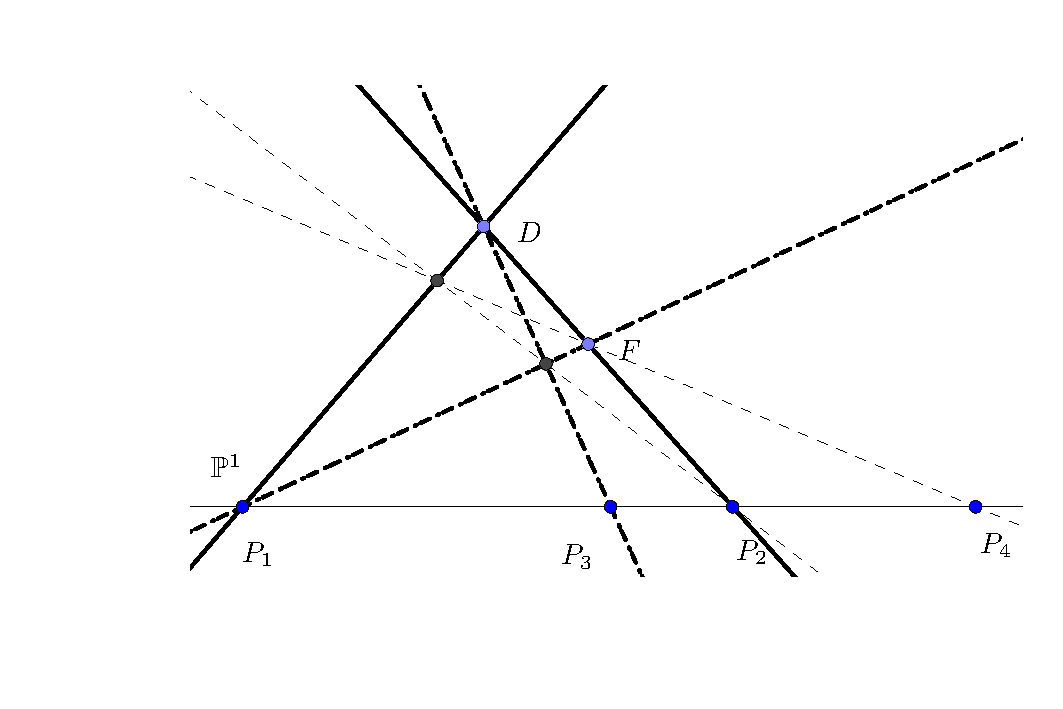
\includegraphics[scale=.6]{Graficos/RazonDoble/razon_doble}
	\caption{Cuaterna armónica}
	\label{C5_img_cuaterna_armonica}
\end{figure}

El recíproco también es cierto, como se muestra en la siguiente proposición.
\begin{prop}
	Dado el cuadrilátero completo formado por los puntos $p_1,p_2,p_3$ y $p_4$, construcción geométrica mostrada en la figura~\ref{C5_img_cuaterna_armonica}, se tiene que $\{p_1,p_2;p_3,p_4\}=-1$.
	
\end{prop}
\begin{proof}
	Tomamos como referencia los puntos $p_1,p_2,D$ y el punto de corte de las rectas $p_1F$ y $p_3D$, que denotaremos $e$. Esto es posible ya que, como se observa en la figura, son proyectivamente independientes.
	\[\mf{R}=\{p_1,p_2,D;e\}\]
	Debemos entonces expresar los puntos $p_1,p_2,p_3$ y $p_4$ respecto a esta referencia. Los primeros son sencillos, $p_1=(1:0:0)$ y $p_2=(0:1:0)$. 
	
	Por otro lado, $p_3$ es la intersección de las rectas $eD$ y $p_1p_2$. Estas pueden ser descritas por las ecuaciones
	\begin{equation*}
		eD:=\class{\alpha(1,1,1)+\beta(0,0,1)\tq \alpha,\beta\in \R}=(1:1:1+\theta)\cup\{D\}\tq\theta\in\R
	\end{equation*}
	\begin{equation*}
		p_1p_2:z=0
	\end{equation*}
	siendo por tanto el punto de corte 
	\[p_3=(1:1:0)\]
	De la misma forma podemos calcular $p_4$ como la intersección de las rectas $p_1p_2$ y $QF$, donde $Q$ es el punto de corte de las rectas $p_1D$ y $p_2e$. Por tanto, para calcular las coordenadas de $p_4$ respecto a la referencia $\mf{R}$, primero debemos obtener las de $Q$ y las de $F$.
	
	Comencemos con $Q$. Las rectas de las cuales es intersección pueden describirse a través de 
	\begin{equation*}
		p_2e:\class{\alpha(1,1,1)+\beta(0,1,0)\tq\alpha,\beta\in \R}=(1:1+\theta:1)\cup\{p_2\}\tq\theta\in\R
	\end{equation*}
	\begin{equation*}
		p_1D:y=0
	\end{equation*}
	por lo que el punto buscado es
	\[Q=(1:0:1)\]
	Para calcular $F$ tenemos que las rectas correspondientes vienen dadas por
	\begin{equation*}
		p_1e:\class{\alpha(1,1,1)+\beta(1,0,0)\tq\alpha,\beta\in \R}=(1+\theta:1:1)\cup\{p_1\}\tq\theta\in\R
	\end{equation*}
	\begin{equation*}
		p_2D:x=0
	\end{equation*}
	siendo el punto de corte
	\[F=(0:1:1)\]
	Podemos ya calcular las coordenadas de $p_4$ como la intersección de 
	\begin{equation*}
		QF:\class{\alpha(1,0,1)+\beta(0,1,1)\tq\alpha,\beta\in \R}=(1:\theta:1+\theta)\cup\{F\}\tq\theta\in\R
	\end{equation*}
	\begin{equation*}
		p_1p_2:z=0
	\end{equation*}
	Con ello obtenemos que
	\[p_4=(1:-1:0)\]
	Una vez hecho esto basta comprobar que la razón doble de $p_1,p_2,p_3$ y $p_4$ es $-1$. Para ello haremos uso de resultados del apartado de cálculo de razones dobles, ya que de momento no hemos visto cómo calcular la razón doble de puntos que no pertenecen a una recta proyectiva, como es el caso.
	
	Entonces, como veremos más adelante
	\begin{equation}
		\{p_1,p_2;p_3,p_4\}=\{(1:0:0),(0:1:0);(1:1:0),(1:-1:0)\}=\{\infty,0;1,-1\}=-1
	\end{equation}
\end{proof}
Dado que en esta construcción las rectas $p_1D$, $p_2D$ y $p_1F$ y los puntos $D$ y $F$ son arbitrarios, elijamos los que elijamos vamos a obtener siempre el mismo punto $p_4$. 

El orden de la cuaterna armónica es relativamente importante ya que, aunque algunas permutaciones cambian su valor, las reordenaciones
\begin{equation*}
	\{p_2,p_1;p_4,p_3\}, \quad \{p_3,p_4;p_1,p_2\}, \quad \{p_2,p_1;p_3,p_4\}
\end{equation*}
siguen dando como resultado $-1$.

Es importante mencionar varias cosas acerca de esta construcción. El punto $p_3$ está entre el punto $p_1$ y el punto medio entre $p_1$ y $p_2$ si y solo si el punto $p_4$ está a la izquierda de $p_1$. Por el contrario, $p_3$ está entre el punto medio y el punto $p_2$  si y solo si el punto $p_4$ está a la derecha de $p_2$. Si el punto $p_3$ no está entre $p_1$ y $p_2$, entonces lo estará $p_4$. Por último, $p_3$ está en el punto medio si y solo si $p_4$ está en el infinito. Esto significa que la recta $p_4F$ es paralela a la recta donde se encuentran los puntos.

Observemos que si, al calcular la razón doble tomamos como referencia los puntos $p_1,p_2,p_3$, entonces, necesariamente, $\theta_4=-1$.
\begin{equation*}
	-1=\{p_1,p_2;p_3,p_4\}=\{\infty,0;1,\theta_4\}=\theta_4
\end{equation*}

\section{Cálculo de la Razón Doble en $\proy^n$}
\label{C5_generalizacionesRazonDoble}
Hasta ahora, sólo hemos calculado la razón doble de cuatro puntos de $\proy^1$. Sin embargo, será útil con frecuencia calcular la razón doble de cuatro puntos alineados en un espacio proyectivo de dimensión finita arbitraria.
 
En esta sección, trataremos de ofrecer procedimientos para realizar estos cálculos de forma eficiente.

Además, para rizar el rizo, y sin salir demasiado de nuestro propósito original, estudiaremos algunas de las relaciones de la razón doble con la dualidad.
\subsection{Razón Doble en $\proy^n$}
En este apartado trataremos de generalizar la noción de razón doble para cuatro puntos alineados de $\proy^n$. Para ello, daremos dos procedimientos distintos que es útil saber dominar. Ambos serán ilustrados con ejemplos (que se recomienda no omitir) para que calen mejor en el lector.
\subsubsection{Procedimiento Referencial}
Sean una recta $r$ de $\proy^n$ y cuatro puntos proyectivos $A,B,C,D\in r$. Para calcular la razón doble de dichos cuatro puntos, tomemos una referencia ``cómoda'' de la recta $r$. De esta forma, los puntos quedan expresados con dos coordenadas homogéneas, pudiendo aplicar los procedimientos de cálculo habituales. Veámoslo con un ejemplo.
\begin{exa}[Cuatro Puntos Alineados]
	\label{C5_exa_puntosAlineados}
	Sean los puntos alineados (compruébese):
	\[\begin{array}{c}
	A=(1:0:-1)=\class{\vec{a}}\\
	B=(2:1:0)=\class{\vec{b}}\\
	C=(4:1:-2)=\class{2\vec{a}+\vec{b}}\\
	D=(-1:-1:-1)=(1:1:1)=\class{\vec{a}-\vec{b}}\\
	\end{array}\]
	Calculemos la razón doble de los mismos. Para ello, tomemos una referencia de la recta $AB$ en la que se encuetran los puntos, por ejemplo: \[\mf{R}=\left\{A,B;\class{\vec{a}+\vec{b}}\right\}\]
	Se comprueba inmediatamente que la base asociada a esta referencia es $\mc{B}=\{\vec{a},\vec{b}\}$.
	
	Obsérvese que, en aras de reducir los cálculos, es recomendable que en la referencia $\mf{R}$ se encuentren el máximo número posible de puntos iniciales. Siempre podemos poner dos de ellos (por ser distintos), pero siempre que se pueda se recomienda poder un tercer punto de los originales como punto unidad (en este caso no era posible). 
	
	A partir de aquí, el cálculo de la razón doble es trivial, ya que, si coordenamos los puntos respecto de la referencia $\mf{R}$ obtenemos:
	\[\{A,B;C,D\}=\{(1:0),(0:1);(2:1),(1:-1)\}\]
	Ahora basta calcular la razón doble por el procedimiento que más nos guste o convenga. En cualquier caso obtenemos el resultado:
	\[\{A,B;C,D\}=\{\infty,0;2,-1\}=\frac{\infty-2}{0-2}:\frac{\infty+1}{0+1}=-\frac{\frac{\infty}{2}}{\frac{\infty}{1}}=-\frac{\cancel{\infty}}{2\cancel{\infty}}=-\frac{1}{2}\]
	Este procedimiento es extremadamente útil cuando la dimensión del espacio ambiente es muy grande ya que de un solo golpe reducirmos el número de componentes de $n$ a $2$.
\end{exa}
\subsubsection{Procedimiento de Proyecciones}
Consideremos ahora una aplicación $h$ entre dos rectas $r$ y $r'$ de $\proy^2$ como la del ejemplo \ref{C4_exa_fabricaHomografias}, es claro que esta proyección es una homografía.

\begin{center}
	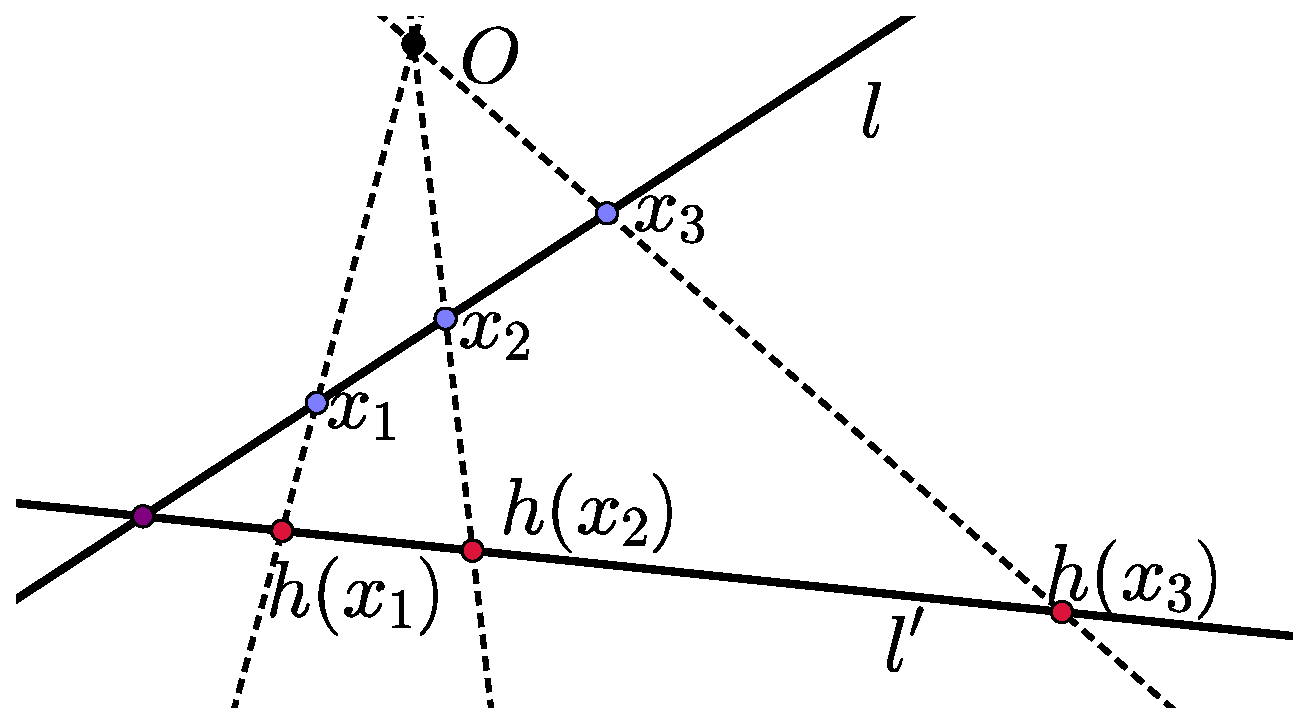
\includegraphics[scale=.3]{Graficos/perspectividad.eps}
\end{center}

Así pues, como las homografías conservan la razón doble, calcular la razón doble de los puntos alineados $A,B,C,D$ será equivalente a calcular la razón doble de sus imágenes por $h$. Es decir:
\[\{A,B;C,D\}=\{h(A),h(B);h(C),h(D)\}\]
La utilidad de esto se ve muy claramente cuando se proyecta sobre los ejes coordenados, tal y como muestra el siguiente ejemplo.
\begin{exa}[Proyección sobre los Ejes]\label{C5:ej_proy_sobre_ejes}
	Sean los puntos $A,B,C,D$ del ejemplo \ref{C5_exa_puntosAlineados}. Tomemos el punto $O=(1:0:0)\not\in AB$ y la recta $r:=AB$. Tomamos asimismo la recta $r'$ definida por la ecuación implícita $x=0$ (eje de coordenadas de $\proy^2$).
	
	Consideramos la proyección $\pi$ del ejemplo \ref{C4_exa_fabricaHomografias}, que a cada punto $x$ de la recta $r$ le asocia el punto intersección de la recta $Ox$ con la recta $r'$. Hallando esta intersección de forma genérica (como aprendimos en \ref{C3_interseccionRectas}) obtenemos la siguiente fórmula explícita para $\pi$:
	\[\begin{array}{c}
	r\setminus\{O\}\stackrel{\pi}{\to} r'\\
	P=(a:b:c)\mapsto\class{(a,b,c)-a(1,0,0)}=(0:b:c)
	\end{array}\]
	De esta forma, como las homografías preservan la razón doble, tenemos que:
	\[\{A,B;C,D\}=\{\pi(A),\pi(B);\pi(C),\pi(D)\}=\{(0:0:-1),(0:1:0);(0:1:-2),(0:1:1)\}\]
	Si ahora consideramos la homografía $\pi'$ que identifica canónicamente a la recta $r'$ con $\proy^1$, dada por la proyección
	\[\begin{array}{c}
	r'\stackrel{\pi'}{\to}\proy^1\\
	x=(0:b:c)\mapsto(b:c)
	\end{array}\]
	de nuevo, como las homografías preservan la razón doble obtenemos:
	\[\{A,B;C,D\}=\{(0:-1),(1:0);(1:-2),(1:1)\}\]
	Y esto ya lo sabemos calcular. Nótese que nos debería dar el mismo resultado que el ejemplo \ref{C5_exa_puntosAlineados}. En efecto:
	\[\{A,B;C,D\}=\left\{0,\infty;-\frac{1}{2},1\right\}=\frac{\frac{1}{2}}{\infty+\frac{1}{2}}:\frac{-1}{\infty-1}=-\frac{1}{2}\]
	Para que la proyección a aplicar sea una homografía es fundamental que el centro de proyección $O$ no pertenezca a la recta en la que los cuatro puntos están alineados.
\end{exa}

La aplicación de uno u otro método (o una combinación de ambos) hace que los cálculos sean mucho más rápidos y sencillos.
\subsection{Razón Doble y Dualidad}
Un paso más en lo que concierne a estas generalizaciones es trasladar todos estos conceptos al espacio dual. Si lo hacemos (estando en $\proy^2$) obtendremos el concepto de razón doble de cuatro rectas concurrentes.

Recordemos que cuatro rectas concurrentes son cuatro rectas que se cortan en un mismo punto. Por tanto, forman un haz de rectas en $\proy^2$ con base el punto de corte. Dado que, como se vio en capítulos anteriores, un haz de rectas en un $\proy^1$ en el espacio proyectivo dual y sabemos calcular la razón doble para puntos de $\proy^1$, si tomamos las rectas como puntos del dual, podremos calcular su razón doble.

Así pues, definimos la razón doble de cuatro rectas concurrentes como la razón doble de los puntos que se corresponden las $4$ rectas en el dual.

Dadas $4$ rectas proyectivas $r_1,r_2,r_3,r_4$ estando cada una de ellas definida por cierta ecuación implícita, se tiene que:
\[r_i:a_ix+b_iy+c_iz=0\]
Sabemos que el punto proyectivo del dual asociado a esa recta es el punto $(a_i:b_i:c_i)$.

De esta forma se tiene que:
\[\{r_1,r_2;r_3,r_4\}=\{(a_1:b_1:c_1),(a_2:b_2:c_2);(a_3:b_3:c_3),(a_4:b_4:c_4)\}\]
Pongamos un ejemplo con rectas concretas para verlo más claro.
\begin{exa}[Razón Doble de Cuatro Rectas Concurrentes]
	Dadas las rectas:
	\[\begin{array}{c}
	r_1:x-y=0\\
	r_2:x+z=0\\
	r_3:2x-y+z=0\\
	r_4:y+z=0
	\end{array}\]
	La razón doble de las mismas, dualizando y proyectando, como vimos en el ejemplo~\ref{C5:ej_proy_sobre_ejes}, queda
	\[\{(1:-1:0),(1:0:1);(2:-1:1),(0:1:1)\}=\{\infty, 0; -1,1\}=-1\]
	Hecho esto, podemos extender el concepto de cuaterna armónica a cuaterca armónica formada por cuatro rectas concurrentes.
\end{exa}
\subsubsection{Método de los Haces de Rectas}
Otra forma de calcular la razón doble de cuatro rectas concurrentes es recurrir a los haces de rectas. Expliquemos esto. Dadas cuatro rectas $r_1,r_2,r_3,r_4$ que se cortan en un mismo punto $O$, consideremos el haz de rectas de base $O$, al que denotaremos por $\haz_O$. Sea otra recta $l$ que no pertenece al haz y consideremos la aplicación proyectiva
\[\begin{array}{cccc}
h:&\haz_O&\rightarrow & l\\
& r&\rightarrow & r\cap l
\end{array}\]

\begin{center}
	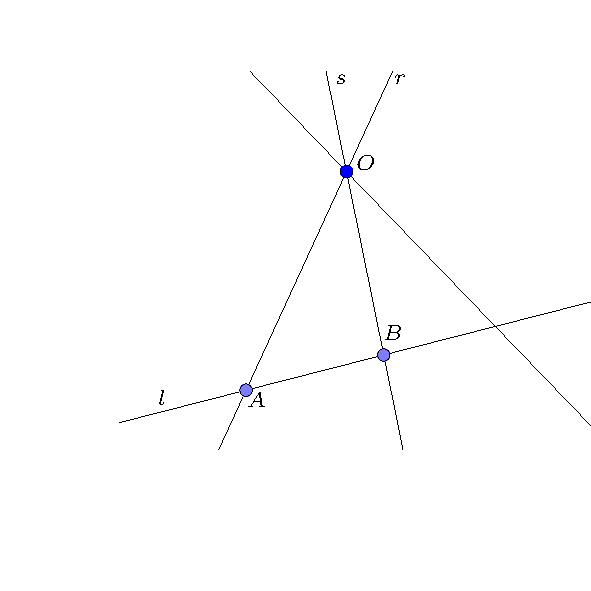
\includegraphics[scale=.8]{Graficos/RazonDoble/rectas_dual}
\end{center}
Si demostramos que $h$ es una homografía, entonces
\begin{equation}
 \{r_1,r_2;r_3,r_4\}=\{h(r_1),h(r_2);h(r_3),h(r_4)\}=\{r_1\cap l,r_2\cap l;r_3\cap l,r_4\cap l\}
\end{equation}
Para ello, veamos cual es la imagen de una recta arbitraria del haz. Es necesario, entonces, parametrizar el haz y tomar una referencia.

Sean $r,s\in\haz_O$ dos rectas distintas del haz y consideremos a referencia $\mf{R}=\{O,h(r),h(s);e\}$ de $\proy^2$. Denotando $h(r)=A$ y $h(s)=B$, la referencia queda $\mf{R}=\{O,A,B;e\}$. Como $h(r)=r\cap l $ y $h(s)=s\cap l$, se tiene que
\[\begin{array}{c}
r_1=lA:z=0\\
s=lB:y=0\\
l=AB:x=0
\end{array}\]
Tomamos entonces como referencia del haz $\mf{\overline{R}}=\{s=[y=0],r=[z=0];[y+z=0]\}$. Así, una recta arbitraria $m\in\haz_O$ puede escribirse como $m:y+\theta z=0$ para cierto $\theta\in\overline{\K}$. De esta forma, $h(m)=m\cap l=(0:-\theta:1)$. Por tanto, la aplicación definida se describe a través de la ecuación $h(\theta)=\theta'=-\theta$ que no es más que una transformación de Möbius. Por tanto, $h$ es una homografía.

Una observación importante es la siguiente.
\begin{lem}
	Cuatro puntos del plano proyectivo $P_1,P_2,P_3,P_4$ forman una cuaterna armónica entonces las rectas $DP_1,DP_2,DP_3,DP_4$ forman una cuaterna armónica de rectas en el dual, donde $D$ es un punto arbitrario.
\end{lem}
\begin{proof}
	Basta fijarse en la construcción del cuadrilátero completo. Tomaremos los mismos nombres de los puntos de corte para que la explicación resulte más sencilla.
	
	Si $P_1,P_2,P_3,P_4$ forman una cuaterna armónica entonces podremos construir un cuadrilátero completo, donde los puntos $D,F$ serán arbitrarios. Si consideramos las rectas $DP_1,DP_2,DP_3,DP_4$, pertenecientes al haz $\haz_D$ y tomamos como recta $l$ la recta $P_1P_2$, se tiene que
	\[\{DP_1,DP_2;DP_3,DP_4\}=\{P_1,P_2;P_3,P_4\}=-1\]
\end{proof}
Esto nos muestra que, cuando tengamos un cuadrilátero completo, no solo formarán una cuaterna armónica los puntos $P_1,P_2,P_3,P_4$, sino también las rectas antes mencionadas.

Por último, veamos un ejemplo.
\begin{exa}
	Consideremos las rectas concurrentes del ejercicio anterior, es decir
	\[\begin{array}{c}
	r_1:x-y=0\\
	r_2:x+z=0\\
	r_3:2x-y+z=0\\
	r_4:y+z=0
	\end{array}\]
	y tomemos como recta $l:x=0$. La razón doble de las cuatro rectas concurrentes es
	 \begin{multline*}
	 	\{r_1,r_2;r_3,r_4\}=\{r_1\cap l,r_2\cap l;r_3\cap l,r_4\cap l\}0\\
	 	=\{(0:0:1),(0:1:0);(0:1:1),(0:1:-1)\}=\{\infty, 0; -1,1\}=-1
	 \end{multline*}
\end{exa}
Este método para calcular la razón doble puede extenderse a un haz de hiperplanos. Análogamente al caso de rectas, si se tienen $\sigma_1,\sigma_2,\sigma_3,\sigma_4$ hiperplanos de $\proy^n$ distintos pertenecientes a un haz de hiperplanos $\haz_\pi$ y sea $r\subset\proy^n$ una recta tal que $r\cap\pi=\emptyset$, entonces
\begin{equation}
	\{\sigma_1,\sigma_2;\sigma_3,\sigma_4\}=\{\sigma_1\cap r,\sigma_2\cap r;\sigma_3\cap r,\sigma_4\cap r\}
\end{equation} 
	\chapter{Clasificación de homografías}
Realizaremos la clasificación de las homografías a partir de sus variedades invariantes. Comenzaremos con las homografías de $\proy^1$, clasificándolas según sus puntos fijos. Relacionaremos esto con las formas canónicas de Jordan y haremos hincapié en algunas homografías importantes, como son las involuciones.

\section{Clasificación de homografías de $\proy^1$. Puntos fijos}
En esta sección haremos una primera aproximación intuitiva a los puntos fijos de una homografía de $\proy^1$, para después enlazarlo con las formas canónicas de Jordan.

Recordemos que podíamos expresar una homografía de $\proy^1$ como
\begin{equation}
	\label{C6_transformada_moebius}
	\theta'=\frac{a\theta+b}{c\theta +d}
\end{equation}
donde $ad-bc\not=0$. Podemos remover un poco las cosas en la ecuación anterior
\begin{equation}
	\theta'(c\theta+d)=a\theta+b\sii c\theta\theta'-a\theta+d\theta'-b=0
\end{equation}
y obtenemos que es equivalente a 
\begin{equation}
	\label{C6_eq_homografia_segundo_orden}
	\alpha\theta\theta'+\beta\theta+\gamma\theta'+\delta=0
\end{equation}
donde $\alpha=c, \ \beta=-a, \ \gamma=d, \ \delta=-b$, denominada \tb{ecuación general} o \tb{implícita} de la homografía.

Que una homografía, distinta de la identidad, mantenga invariante un punto $(x,y)$ implica que $(x',y')=(x,y)$ y con ello $\theta'=\theta$. Sustituyendo en la ecuación anterior obtenemos una ecuación de segundo grado, y, por tanto, tendrá dos soluciones distintas o una solución doble. Esto quiere decir que, suponiendo que $\K=\C$, las homografías, exceptuando la identidad, tienen dos puntos fijos distintos o un punto fijo doble, dependiendo de la ecuación resultante.
\begin{equation}
	\label{C6_eq_homografia_segundo_orden_punto_fijo}
	\alpha\theta^2+(\beta+\gamma)\theta+\delta=0
\end{equation}
Veamos en cada uno de los casos cuál es la expresión de la homografía que tiene esos puntos fijos, basándonos en la ecuación anterior.

\subsection{Dos puntos fijos distintos}
Sea $h$ una homografía de $\proy^1$ con dos puntos fijos $M$ y $N$ distintos. Tratamos de encontrar el valor de los parámetros $\alpha, \beta,\gamma,\delta$ para poder describir las homografías de este tipo. Como sabemos que $M$ y $N$ son puntos fijos, sus coordenadas no homogéneas deben cumplir la ecuación~\eqref{C6_eq_homografia_segundo_orden_punto_fijo}. Por tanto, una forma de hallar estos parámetros sería sustituir las coordenadas no homogéneas de los puntos fijos en dicha ecuación y ver para que valores de $\alpha, \beta,\gamma,\delta$ se cumple. 

Para facilitar este cálculo tomamos la referencia $\mf{R}=\{M,N;e\}$, donde $e$ es un punto cualquiera distinto de $M$ y $N$. En esta referencia las coordenadas no homogénea de $M$ y $N$ son $\infty$ y $0$, respectivamente. Por tanto, la ecuación~\eqref{C6_eq_homografia_segundo_orden_punto_fijo} admite como soluciones $0$ y $\infty$. Sustituyendo estos valores en la ecuación obtenemos que 
\begin{equation*}
	\alpha\cdot 0+(\beta+\gamma)0+\delta=0\sii\delta=0
\end{equation*}
Hagamos el cálculo para $\infty$ con más cuidado. Sustituyendo las coordenadas no homogéneas por las coordenadas homogéneas en la ecuación~\eqref{C6_eq_homografia_segundo_orden}, esta queda
\begin{equation}
	\alpha xx'+\beta xy'+\gamma x'y+\delta yy'=0
\end{equation}
Dado que estamos con puntos fijos imponemos que $(x',y')=(x,y)$ y que $\delta=0$, pues lo hemos hallado antes
\begin{equation*}
	\alpha x^2+\beta xy+\gamma xy=0
\end{equation*}
Las coordenadas homogéneas de $M$ respecto a la referencia $\mf{R}$ son $(1:0)$. Sustituyéndolas en la ecuación anterior obtenemos que
\begin{equation*}
\alpha 1+\beta 0+\gamma 0=0\sii \alpha=0
\end{equation*}
Por tanto, en una homografía de $\proy^1$ con dos puntos fijos se tiene que $\alpha=c=0$ y $\delta=-b=0$. Entonces, la \ti{ecuación canónica} de la homografía respecto a la referencia $\mf{R}$ tomada es
\begin{equation}
	\theta'=\frac{a\theta+b}{c\theta +d}=\frac{a}{d}\theta=k\theta
\end{equation}
donde la constante $k$ se llama \tb{módulo de la homografía}. Notemos que dada cualquier homografía que tenga dos puntos fijos distintos, tomando la referencia adecuada, podemos decir que dichos puntos fijos son el cero y el infinito.

\begin{obs}
	El cálculo para el punto $M$, cuya coordenada no homogénea era $\infty$, puede hacerse sin tener tanto cuidado, gracias a que hemos comprobado rigurosamente que funciona.
	\begin{equation*}
		\alpha\theta^2+(\beta+\gamma)\theta+\delta=0\ra\alpha+(\beta+\gamma)\frac{1}{\theta}+\delta\frac{1}{\theta^2}=0
	\end{equation*}
	\begin{equation*}
		\alpha+(\beta+\gamma)\frac{1}{\infty}+\delta\frac{1}{\infty^2}=0\sii \alpha=0
	\end{equation*}
\end{obs}
Es importante observar que, aunque la ecuación $\theta'=k\theta$ se denomina canónica, en realidad no lo es mucho, ya que esta expresión se ha obtenido tomando la referencia $\mf{R}=\{M,N;e\}$. Notemos que si en vez de tomar como referencia $\mf{R}$ tomamos $\overline{\mf{R}}=\{N,M;e\}$, la ecuación cambia.

En efecto, el cambio de $\mf{R}$ a $\overline{\mf{R}}$ viene dado por la homografía que trasforma $(1:0)$ en $(0:1)$ y $(0:1)$ en $(1:0)$. Sustituyendo estas trasformaciones, en coordenadas no homogéneas, en la ecuación~\eqref{C6_transformada_moebius}, obtenemos que la ecuación de la homografía que transforma $\mf{R}$ en $\overline{\mf{R}}$ es
\begin{equation*}
	\overline{\theta}=\frac{b}{c\theta}=\frac{\lambda}{\theta}
\end{equation*}
Por tanto, la ecuación $\theta'=k\theta$ respecto a la referencia $\overline{\mf{R}}$, que se obtiene despejando en la ecuación anterior $\theta$ en función de $\overline{\theta}$ y sustituyendo, es
\begin{equation*}
	\frac{\lambda}{\overline{\theta}'}=k\frac{\lambda}{\overline{\theta}}\sii \overline{\theta}'=\frac{1}{k}\overline{\theta}
\end{equation*}
por lo que en este caso el módulo de la homografía con puntos fijos $M$ y $N$ sería $1/k$. 

Podríamos preguntarnos entonces porque darle el apellido canónico. Aunque una permutación de los puntos $M$ y $N$ en la referencia nos da un valor del módulo de la homografía distinto, el parámetro $k$ está geométricamente asociado a la homografía, cosa que veremos no ocurrirá con parámetros posteriores. Es decir, solo está ligado a la homografía y al orden de los puntos $M$ y $N$ en la referencia, y dependiendo de este obtendremos $k$ o $1/k$. Observemos que no depende del punto unidad $e$ que hayamos tomado. Por tanto, la ecuación
\begin{equation}
	\label{C6_theta_ktheta}
	\theta'=k\theta
\end{equation}
puede considerarse canónica.

El parámetro $k$ puede ser hallado a través de la razón doble, ya que estamos tratando homografías. En efecto, dada una homografía $h$ que deja fijos los puntos $M$ y $N$ y, por tanto, en la referencia $\mf{R}=\{M,N;e\}$ viene descrita por la ecuación~\eqref{C6_theta_ktheta} para cierto $k$, se tiene que
\begin{equation}
	\{M,N,P,h(P)\}=\{\infty,0,\theta,\theta'=k\theta\}=k
\end{equation}
para un punto $P$ cualquiera independientemente de $e$. Si permutamos los puntos $M$ y $N$, por la simetría de la razón doble se tiene que
\begin{equation}
	\{N,M,P,h(P)\}=\frac{1}{k}
\end{equation}
independientemente de $e$. Esto nos demuestra de nuevo que el módulo depende solo de la homografía y del orden de los puntos fijos.

Hagamos un pequeño inciso que retomaremos más adelante. Si escribimos, en la referencia $\mf{R}=\{M,N,e\}$, la matriz asociada a una homografía $h$ que tiene dos puntos fijos $M$ y $N$ obtenemos
\begin{equation*}
	\left( \begin{array}{cc}
	a&0\\
	0&d
	\end{array}\right) 
	\sim \left( \begin{array}{cc}
	\frac{a}{d}&0\\
	0&1
	\end{array}\right) 
	\sim \left( \begin{array}{cc}
	k&0\\
	0&1
	\end{array}\right)
\end{equation*}
Por tanto, hemos encontrado una referencia en la cual la homografía $h$ es diagonal. Notemos que, además, el módulo de la homografía es el cociente de los autovalores.

\subsection{Un punto fijo doble}
Veamos ahora qué ecuación describe a una homografía $h$ de $\proy^1$ que deja fijo un solo punto. Si $M$ es el punto fijo de $h$, entonces la ecuación~\eqref{C6_eq_homografia_segundo_orden_punto_fijo} debe admitir como solución la coordenada no homogénea de $M$. Por tanto, procederemos como en el caso anterior. Tomaremos una referencia adecuada y sustituiremos la coordenada no homogénea de $M$, respecto a dicha referencia, en la ecuación~\eqref{C6_eq_homografia_segundo_orden_punto_fijo} para hallar los parámetros $\alpha, \beta,\gamma,\delta$.

Dado que solo hay un punto fijo, tomamos como referencia $\mf{R}=\{M,X;e\}$, donde $X$ y $e$ son puntos diferentes y distintos de $M$. En esta referencia la coordenada no homogénea de $M$ es $\infty$. Por tanto, para cualquier homografía con un punto fijo doble, tomando la referencia adecuada, se puede decir que dicha homografía deja fijo el infinito. Dado que ya justificamos anteriormente los cálculo con $\infty$ esta vez lo haremos sin tener cuidado. Recordemos que podíamos escribir
\begin{equation*}
	\alpha\theta^2+(\beta+\gamma)\theta+\delta=0\ra\alpha+(\beta+\gamma)\frac{1}{\theta}+\delta\frac{1}{\theta^2}=0
\end{equation*}
\begin{equation*}
	\alpha+(\beta+\gamma)\frac{1}{\infty}+\delta\frac{1}{\infty^2}=0\sii \alpha=0
\end{equation*}
Por tanto la ecuación que describe los puntos fijos de la homografía pasa a ser
\begin{equation*}
	(\beta+\gamma)\theta+\delta=0
\end{equation*}
Dado que el punto $M$ es solución doble de la ecuación de segundo grado~\eqref{C6_eq_homografia_segundo_orden_punto_fijo}, si volvemos a sustituir su coordenada no homogénea en la ecuación anterior, esta debe cumplirse. Por tanto
\begin{equation*}
	(\beta+\gamma)\theta+\delta=0\ra(\beta+\gamma)+\delta\frac{1}{\theta}=0
\end{equation*}
\begin{equation*}
	(\beta+\gamma)+\delta\frac{1}{\infty}=0\sii \beta=-\gamma
\end{equation*}
Por tanto, en una homografía de $\proy^1$ con un punto fijo doble se tiene que $\alpha=c=0$ y $-a=\beta=-\gamma=-d$. Entonces, la ecuación ``canónica" de la homografía, respecto a la referencia $\mf{R}$ tomada, es
\begin{equation}
\theta'=\frac{a\theta+b}{c\theta +d}=\frac{a\theta+b}{a}=\theta+\mu
\end{equation}
A este tipo de homografías de las denomina \ti{elaciones} y se dice que dejan fijo el infinito pues, como hemos visto antes, tomando la referencia adecuada el punto fijo $M$ pasa a ser $\infty$.

Notemos que esta vez el apellido canónico no es merecido, al contrario que en el caso anterior, pues el parámetro $\mu$ no está geométricamente asociado a la homografía. 

Veámoslo. Partiendo de la referencia $\mf{R}=\{M,X;e\}$, realizamos un cambio de coordenadas que lleve el infinito al infinito. Por ejemplo, aplicamos una homografía con ecuación
\begin{equation*}
	\overline{\theta}=\frac{1}{k}\theta
\end{equation*}
es decir, una homografía $h$ que en esa referencia deje fijos el cero y el infinito. Por tanto, estamos pasando de la referencia $\mf{R}$ a la referencia $\overline{\mf{R}}=\{M,X;h(e)\}$. 

La ecuación $\theta'=\theta+\mu$ respecto a la referencia $\overline{\mf{R}}$, que se obtiene despejando en la ecuación anterior $\theta$ en función de $\overline{\theta}$ y sustituyendo, es
\begin{equation*}
	k\overline{\theta'}=k\overline{\theta}+\mu\sii \overline{\theta'}=\overline{\theta}+\frac{\mu}{k}
\end{equation*}
Si $k=\mu$ entonces la ecuación de una homografía cuyo punto fijo es $M$ respecto a la referencia $\overline{\mf{R}}$ es
\begin{equation*}
	\overline{\theta}'=\overline{\theta}+1
\end{equation*}
Como se puede observar, el parámetro $\mu$ no está asociado a la homografía, pues lo hemos eliminado de la ecuación que la define. Por tanto, la ecuación $\theta'=\theta+\mu$ no se puede considerar canónica. Lo máximo a lo que podemos aspirar es a expresar la ecuación de una elación como $\theta'=\theta+1$, tomando la referencia adecuada.

De nuevo, hagamos un inciso que retomaremos más adelante. Dada una homografía $h$ que tiene un punto fijo doble $M$, si escribimos, en la referencia $\mf{R}$ en la cual la ecuación que la define es $\theta'=\theta+1$ (y por tanto $b=a$), su matriz asociada obtenemos
\begin{equation*}
\left( \begin{array}{cc}
a&a\\
0&a
\end{array}\right) 
\sim \left( \begin{array}{cc}
1&1\\
0&1
\end{array}\right) 
\end{equation*}
Por tanto, hemos encontrado una referencia en la cual la matriz de la homografía $h$ se encuentra en su forma canónica de Jordan, salvo múltiplo.

\section{Formas canónicas de Jordan y puntos fijos}
Hemos anticipado que existe cierta relación entre los puntos fijos de una homografía y la forma canónica de Jordan de su matriz asociada. En este apartado explicaremos cuál es esa relación.\\

Sea $h$ una homografía distinta de la identidad. Si un punto $[v]$ es punto fijo de la homografía, entonces 
\begin{equation}
	\label{C6_eq_puntofijo_autovector}
	[\widehat{h}(v)]=h([v])=[v]\sii \widehat{h}(v)=\rho v
\end{equation}
para cierto $\rho$, de lo cual se deduce que $v$ es autovector de la aplicación lineal $\widehat{h}$ con autovalor asociado $\rho$. Por tanto, un punto $x$ es punto fijo de la homografía si y solo si es un autovector de la aplicación lineal $\widehat{h}$, asociado a un autovalor no nulo.

Antes de continuar hagamos un pequeño recordatorio.

\begin{obs}
	Dada un endomorfismo $\widehat{h}$ de $E$ ($\dim(E)=n$) y sean $\lambda_i$, con $i=1,\cdots,r$ sus distintos autovalores, se llama subespacio propio asociado a $\lambda_i$ al subesapcio vectorial $V_{\lambda_i}$ formado por todos los autovectores asociados a dicho autovalor:
	\begin{equation}
		V_{\lambda_i}:=\{u\in E\tq \widehat{h}(u)=\lambda_i u\}
	\end{equation}
	Se verifica que 
	\begin{equation}
		V_{\lambda_i}= \ker(\widehat{h}-\lambda_i I) \ ; \quad \dim(V_{\lambda_i})=n-rg(A-\lambda_i I)
	\end{equation}
	donde $A$ es la matriz asociada a $\widehat{h}$. 
	
	La dimensión de $V_{\lambda_i}$, denotada por $d_i$ se denomina multiplicidad geométrica. Por otro lado, la multiplicidad de $\lambda_i$ como raíz del polinomio característico se denomina multiplicidad algebraica, y se denota por $\alpha_i$. Si $\alpha_i+\cdots+\alpha_r=n$ y $d_i=\alpha_i$ para cada $i=1,\cdots,r$, entonces $\widehat{h}$ es diagonalizable. En el caso en el que solo se cumpla que $\alpha_i+\cdots+\alpha_r=n$ el endomorfismo será ``Jordanizable".
\end{obs}

Sabemos pues que $u$ es autovector de $\widehat{h}$ asociado a un autovalor $\lambda$ no nulo si y solo si $[u]$ es punto fijo. Por tanto, como $V_{\lambda}$ está formado por todos los autovectores asociados a $\lambda$, se tiene que $\proy(V_\lambda)$ es una variedad proyectiva formada por punto fijos de $h$. Además, el conjunto de las proyecciones de los subespacios propios asociados a los distintos autovalores de $\widehat{h}$ nos proporcionan todos los puntos fijos de $h$.

Notemos que hasta ahora no hemos utilizado en absoluto que $h$ sea una homografía de $\proy^1$. Con esto queremos resaltar que todo lo dicho es válido para homografías de $\proy^n$. Es decir, los puntos fijos de una homografía de $\proy^n$ vienen dados por $\proy(V_{\lambda_i})$ para los distintos autovalores $\lambda_i$ de la aplicación lineal asociada.

\begin{obs}
	Cualquier homografía de un espacio proyectivo complejo tiene puntos fijos. Sin embargo, hay homografías del espacio proyectivo real que no los tienen. Podemos precisar un poco más, ya que sabemos que todo polinomio con coeficientes en $\R$ de grado impar tiene raíces. Por tanto para que haya homografías sin puntos fijos, el grado del polinomio debe ser par, con lo cual la dimensión del espacio vectorial es par y, por tanto, la dimensión del espacio proyectivo debe ser impar. A no ser que se diga lo contrario, de aquí en adelante trabajaremos en $\C$.
\end{obs}

Indaguemos un poco más para obtener las conclusiones del apartado anterior, es decir, que una homografía $h$ de $\proy^1$ distinta de la identidad tiene o dos puntos fijos distintos o uno doble. Para ello trabajemos con matrices.\\

Sea $A$ la matriz asociada a la homografía $h$, que no es más que la matriz asociada a la aplicación lineal $\widehat{h}$, y $x$ un punto fijo de $h$. Entonces $\rho x=Ax$, con lo cual se obtiene el sistema $(A-\rho I)x=0$, que tiene solución no idénticamente nula si y solo si $\det(A-\rho I)=0$. Este determinante no es otro que el polinomio característico, cuyas raíces, $\rho$, son los autovalores de la aplicación lineal $\widehat{h}$. Dado que nos encontramos en $\proy^1$, la matriz $A$ será una matriz $2\times 2$, y, por tanto, el polinomio característico será un polinomio de segundo grado. Esto implica que tendrá dos soluciones distintas o una solución doble, siempre que el cuerpo sobre el que estemos trabajando se $\C$. Consecuentemente, la aplicación lineal $\widehat{h}$ tendrá un autovalor o dos distintos. Evaluemos cada caso:
\begin{enumerate}
	\item Si $\widehat{h}$ tiene dos autovalores distintos, entonces $\dim(V_{\rho_i})=1$. Por tanto, las variedades proyectivas $\proy(V_{\rho_1})$ y $\proy(V_{\rho_2})$ tienen dimensión cero, por lo que son puntos. Esto da lugar a dos puntos fijos distintos en la homografía. Además si escribimos la matriz $A$ en la base formada por estos dos autovectores obtendremos una matriz diagonal, como habíamos visto antes.
	
	\item Si $\widehat{h}$ tiene un solo autovalor $\rho$, en cuyo caso $\alpha_1=2$, en principio pueden darse dos casos.
	\begin{itemize}
		\item El caso en el que $\dim(V_{\rho})=2=d_1$ no es admisible, ya que hemos supuesto que $h$ es distinta de la identidad. Sin embargo, la aplicación $\widehat{h}$ con $\dim(V_{\rho})=2$ tiene como autovectores asociados a $\rho$ todo el espacio vectorial, por lo que todos los puntos de $\proy^1$ serían puntos fijos de $h$.
		
		\item Si $\dim(V_{\rho})=1=d_1$ entonces $\proy(V_{\rho})$ es un punto. En tal caso, la homografía $h$ tendrá un único punto fijo doble. Además, dado que $\alpha_1=2\not=d_1=1$, la matriz $A$ no es diagonalizable. Sin embargo, sí admite forma canónica de Jordan. Por tanto, en cierta base, a la cual pertenece dicho autovector, la matriz $A$ se encuentra en su forma canónica de Jordan, como vimos anteriormente.
	\end{itemize}
\end{enumerate}
Con todo ello podemos concluir que una homografía de $\proy^1$, distinta de la identidad, tiene dos puntos fijos distintos o un punto fijo doble. Si escribimos la matriz asociada a la homografía en la base dada por dichos puntos fijos obtendremos, en el primer caso, una matriz diagonal y, en el segundo, su forma canónica de Jordan. 
\begin{obs}
	Sea una homografía $h$ de $\proy^1$ y su aplicación lineal asociada $\widehat{h}$. Un punto $[v]$ de $\proy^1$ pertenece al centro de $h$ si y solo si es un autovector de $\widehat{h}$ con autovalor $0$.
	
	En efecto, que $[v]$ esté en el centro de $h$ equivale a que $v\in \ker\widehat{h}$, es decir, que $\widehat{h}(v)=0=0\cdot v$.
\end{obs}

\section{Aplicaciones afines}
En esta sección y en la que sigue trataremos algunos casos particulares, de gran importancia, de homografías de $\proy^1$.

Estudiemos las homografía de $\proy^1$ tales que su matriz asociada es
\begin{equation*}
	A=\left( \begin{array}{cc}
		a&b\\
		0&d
	\end{array}\right)
\end{equation*}
es decir, $c=0$, y con ello , como $d$ no puede ser cero, 
\begin{equation}
	\theta'=\frac{a\theta+b}{d}=\alpha\theta+\beta
\end{equation}
donde $\alpha=a/d$ y $\beta=b/d$. Veamos cuáles son sus puntos fijos.\\

Siguiendo lo visto en el apartado anterior, debemos encontrar los autovalores de $A$ y sus autovectores asociados. Realizando unas sencillas cuentas se llega a que los autovalores son $a$ y $d$. Dado que hay dos autovalores distintos, la homografía $h$ tendrá dos puntos fijos. 

Calculemos dos autovectores, $u_a$ y $u_d$ asociados a estos autovalores. Recordemos que, como $V_{\lambda}= \ker(\widehat{h}-\lambda I)$, si $u$ es un autovector con autovalor $\lambda$, entonces $u\in V_{\lambda}= \ker(\widehat{h}-\lambda I)$, y, por tanto, $(A-\lambda I)u=0$. Esto nos proporciona una forma de hallar los autovectores. En nuestro caso
\begin{equation*}
	(A-a I)\left( \begin{array}{c}
	x\\
	y
	\end{array}\right)=\left( \begin{array}{cc}
	0&b\\
	0&d-a
	\end{array}\right)
	\left( \begin{array}{c}
	x\\
	y
	\end{array}\right)=\left( \begin{array}{c}
	0\\
	0
	\end{array}\right)\sii y=0\ra u_{a}=(1,0)
\end{equation*}
\begin{equation*}
	(A-d I)\left( \begin{array}{c}
	x\\
	y
	\end{array}\right)=\left( \begin{array}{cc}
	a-d&b\\
	0&0
	\end{array}\right)
	\left( \begin{array}{c}
	x\\
	y
	\end{array}\right)=\left( \begin{array}{c}
	0\\
	0
\end{array}\right)\sii y=\frac{a-d}{b}x\ra u_b=(b,d-a)
\end{equation*}
Por tanto, los dos puntos fijos de la homografía $h$ son $(1:0)$ y $(b/d:1-a/d)=(\beta:1-\alpha)$, cuyas coordenadas no homogéneas son $\infty$ y $\frac{\beta}{1-\alpha}$. 

Dado que la ecuación $\theta'=\alpha\theta+\beta$ define una aplicación afín de la recta podemos concluir que \tb{las afinidades}, homografías con $c=0$, \tb{dejan fijo el infinito}. 
\begin{obs}
	No se deben confundir estas con las elaciones. Mientras las elaciones tienen un punto fijo doble, que se puede identificar con el infinito en cierta referencia, las homografías con $c=0$ dejan fijo el infinito sea cual sea la referencia en la que nos encontramos. Es decir, si cambiamos de referencia seguirán teniendo como punto fijo el punto $(1:0)$ de dicha referencia.
\end{obs}
Veamos el \tb{recíproco}, si una homografía de $\proy^1$ deja fijo el infinito, entonces es una aplicación afín. 

Sea una homografía de $\proy^1$ con matriz asociada
\begin{equation*}
	A=\left( \begin{array}{cc}
		a&b\\
		c&d
	\end{array}\right)
\end{equation*}
Si deja fijo el infinito, entonces
\begin{equation*}
	\left( \begin{array}{cc}
	a&b\\
	c&d
	\end{array}\right)
	\left( \begin{array}{c}
	1\\
	0
	\end{array}\right)=\rho\left( \begin{array}{c}
	1\\
	0
	\end{array}\right)\sii a=\rho \ , \ c=0
\end{equation*}
Por tanto, la matriz de la homografía, dado que $d\not=0$, es
\begin{equation*}
	A=\left( \begin{array}{cc}
		a&b\\
		0&d
	\end{array}\right)\sim 
	\left( \begin{array}{cc}
		\alpha&\beta\\
		0&1
	\end{array}\right)
\end{equation*}
Si describimos la homografía que deja fijo el infinito a través de la transformación de Möbius obtenemos que 
\begin{equation*}
	\theta'=\alpha\theta+\beta
\end{equation*}
es decir, es una transformación afín de la recta.\\

Estos dos resultados dan lugar al siguiente lema.
\begin{lem}\label{C6_lem_infinito_p1_sii_afinidad}
	Dada una homografía de $\proy^1$ y $\mf{R}=\{x_0,x_1;e\}$ una referencia arbitraria. Entonces $h$ deja fijo el infinito, es decir, deja fijo el punto $x_0$, si y solo si $c=0$, o equivalentemente, si y solo si es una afinidad.
\end{lem}

El cálculo de los puntos fijos de la homografía de $\proy^1$ dada al principio de esta sección, aquella cuya matriz asociada es
\begin{equation*}
	A=\left( \begin{array}{cc}
		a&b\\
		0&d
	\end{array}\right)
\end{equation*}
y que viene descrita a través de la ecuación
\begin{equation*}
	\theta'=\alpha\theta+\beta
\end{equation*}
podría haberse hecho como se hizo en el primer apartado de este capítulo, cuando aún no conocíamos la relación entre los puntos fijos y los autovectores.

En tal caso, tendríamos que buscar las coordenadas no homogéneas $\theta$ que cumplen la ecuación
\begin{equation*}
	\theta=\alpha\theta+\beta
\end{equation*}
Sin embargo, esta ecuación, dado que es de primer orden, solo tiene una solución, pero sabemos que el $\infty$, es decir el $(1:0)$, es también punto fijo de $h$. Por tanto, debe cumplir también la ecuación. Si hacemos la comprobación con las coordenadas no homogéneas obtenemos que 
\begin{equation*}
	\infty=\alpha\infty+\beta=\infty
\end{equation*}
Sin embargo, personalmente, esta comprobación no me tranquiliza, dado que es un procedimiento falto de rigor. Por tanto, vamos a comprobarlo de nuevo con las coordenadas homogéneas. En tal caso tenemos la ecuación
\begin{equation}
	\label{C6_puntofijo_malcalculo}
	\frac{x'}{y'}=\alpha\frac{x}{y}+\beta
\end{equation}
\begin{equation}
	\label{C6_puntofijo_buencalculo}
	x'y=\alpha xy'+\beta yy'
\end{equation}
Imponiendo que $(x,y)$ es punto fijo obtenemos 
\begin{equation*}
	 xy=\alpha xy+\beta y^2\sii xy-\alpha xy-\beta y^2=0
\end{equation*}
Una simple comprobación nos permite asegurar que el punto $(1:0)$ es punto fijo de $h$
\begin{equation*}
	1\cdot 0-\alpha\cdot 1\cdot 0+\beta\cdot 0=0
\end{equation*}
\begin{obs}
	Si en vez imponer la condición de punto fijo, $(x,y)=(x',y')$, en la ecuación~\eqref{C6_puntofijo_buencalculo} lo hacemos en la ecuación~\eqref{C6_puntofijo_malcalculo} y luego multiplicamos por $y$, el punto $(1:0)$ solo es solución de la ecuación resultante si $\alpha=1$, cuando debería serlo para todo $\alpha$.
	\begin{equation*}
		\frac{x}{y}=\alpha\frac{x}{y}-\beta\sii x=\alpha x+\beta y
	\end{equation*}
	\begin{equation*}
		 1=\alpha 1+\beta 0=\alpha
	\end{equation*}
	Esto nos muestra que trabajar con las coordenadas no homogéneas y pasar después a homogéneas tiene sus limitaciones, y siempre que hagamos cálculos de este estilo debemos tener bien claro qué estamos haciendo.
\end{obs}

\subsection{Aplicaciones afines y homografías de $\proy^n$}
El lema~\ref{C6_lem_infinito_p1_sii_afinidad} se puede generalizar a una homografía de $\proy^n$. A continuación expondremos y demostraremos dicho resultado.

\begin{prop}
	Sea $h$ una homografía de $\proy^n$ y $\mf{R}=\{x_0,\cdots,x_n;e\}$ una referencia arbitraria. El hiperplano $H$ dado por la ecuación implícita $x_n=0$ se denomina plano del infinito. Si $h$ deja invariante el plano del infinito entonces es una aplicación afín.
\end{prop}
\begin{obs}
	Que una homografía deje invariante un hiperplano $H$ no significa que deje invariante cada punto del hiperplano, es decir, que los puntos de $H$ sean puntos fijos, sino que la imagen de un punto de $H$ pertenece al hiperplano, pero no tiene por qué ser el mismo punto.
\end{obs}
\begin{proof}
	Sea $h:\proy^n\rightarrow \proy^n$ una homografía que deja invariante el plano $H$ dado por la ecuación $x_n=0$. La matriz asociada a dicha aplicación vendrá dada por
	\begin{equation*}
		\left( \begin{array}{ccc}
			a_{00}&\cdots&a_{0n}\\
			a_{10}&\cdots&a_{1n}\\
			\vdots&\ddots&\vdots\\
			a_{n0}&\cdots&a_{nn}
		\end{array}\right) 
	\end{equation*}
	para ciertos $a_{ij}$, con $i,j=0,\cdots,n$. Dado un punto $(x_0:\cdots:x_n)$ su imagen vendrá dada por la clase del vector $(x_0',\cdots,x_n')$ tal que
	\begin{equation*}
		\left( \begin{array}{ccc}
			a_{00}&\cdots&a_{0n}\\
			a_{10}&\cdots&a_{1n}\\
			\vdots&\ddots&\vdots\\
			a_{n0}&\cdots&a_{nn}
		\end{array}\right) 
		\left( \begin{array}{c}
			x_0\\
			x_1\\
			\vdots\\
			x_n
		\end{array}\right) =\rho
		\left( \begin{array}{c}
			x_0'\\
			x_1'\\
			\vdots\\
			x_n'
		\end{array}\right)
	\end{equation*}
	Los vectores pertenecientes a $\widehat{H}$ tienen la forma $(x_0,\cdots,x_{n-1},0)$. Dado que $h$ deja invariante el hiperplano $H$ debe cumplirse que
	\begin{equation*}
		\left( \begin{array}{ccc}
			a_{00}&\cdots&a_{0n}\\
			a_{10}&\cdots&a_{1n}\\
			\vdots&\ddots&\vdots\\
			a_{n0}&\cdots&a_{nn}
		\end{array}\right) 
		\left( \begin{array}{c}
			x_0\\
			\vdots\\
			x_{n-1}\\
			0
		\end{array}\right) =\rho
		\left( \begin{array}{c}
			x_0'\\
			\vdots\\
			x_{n-1}'\\
			0
		\end{array}\right)
	\end{equation*}
	Por tanto, debe cumplirse la ecuación
	\begin{equation*}
		a_{n0}x_0+\cdots+a_{nn-1}x_{n-1}+a_{nn}\cdot0=\rho\cdot0=0
	\end{equation*}
	para todo $(x_0,\cdots,x_{n-1})\not=(0,\cdots,0)$. Esto implica que, necesariamente
	\begin{equation*}
		a_{n0}=0=a_{n1}=\cdots=a_{nn-1}
	\end{equation*}
	con lo que la matriz asociada a $h$ adopta la forma
	\begin{equation*}
		\left( \begin{array}{cccc}
			a_{00}&\cdots&a_{0n-1}&a_{0n}\\
			a_{10}&\cdots&a_{1n-1}&a_{1n}\\
			\vdots&\ddots&\vdots&\vdots\\
			0&\cdots&0&a_{nn}
		\end{array}\right) 
	\end{equation*}
	Dado que $a_{nn}\not=0$, pues debe ser invertible, la matriz se puede expresar, usando bloques, como
	\begin{equation*}
		\left( \begin{array}{ccc|c}
			&&&\\
			&A&&b\\
			&&&\\ \hline
			0&\cdots&0&1
		\end{array}\right) =
		\left( \begin{array}{ccc|c}
			&&&\\
			&A&&b\\
			&&&\\ \hline
			&0^t&&1
		\end{array}\right)
	\end{equation*}
	Veamos cuál es la expresión de una homografía de $\proy^n$ con esta matriz asociada. Dado un punto $p=(x_0:\cdots:x_{n-1}:x_n)\not\in H$, es decir, tal que $x_n\not=0$, podemos escribirlo como
	\begin{equation*}
		p=(x_0:\cdots:x_{n-1}:x_n)=\left( \frac{x_0}{x_n}:\cdots:\frac{x_{n-1}}{x_n}:1\right) =(X_0:\cdots:X_{n-1}:1)=
		\left( \begin{array}{c}
			\\
			X\\
			\\
			1
		\end{array}\right)^t
	\end{equation*}
	donde $X_i=\frac{x_i}{x_n}$ para $i=0,\cdots,n-1$. Entonces
	\begin{equation*}
		\left( \begin{array}{ccc|c}
			&&&\\
			&A&&b\\
			&&&\\ \hline
			&0^t&&1
		\end{array}\right)
		\left( \begin{array}{c}
			\\
			X\\
			\\
			1
		\end{array}\right)=
		\left( \begin{array}{c}
			\\
			AX+b\\
			\\
			1
		\end{array}\right)=
		\left( \begin{array}{c}
			\\
			X'\\
			\\
			1
		\end{array}\right)
	\end{equation*}
	Con ello, la homografía $h$ que deja fijo el plano del infinito $H$ viene descrita por
	\begin{equation}
		h:X'=AX+b
	\end{equation}
	siendo por tanto $h$ una aplicación afín.
\end{proof}

\section{Involuciones}
En esta sección introduciremos un tipo de homografías, llamadas involuciones, que serán de gran importancia a la hora de estudiar cónicas.
\begin{defi}
	Dada una homografía $h$ de $\proy^1$, distinta de la identidad, se dice que es una \ti{involución} si $h^2=id$.
\end{defi}
Estudiemos cómo se caracterizan las involuciones y cómo describirlas.
\begin{lem}
	Dada una homografía $h$ de $\proy^1$ distinta de la identidad. Existe un punto $P\in\proy^1$ tal que $h(P)\not=P$ y $h^2(P)=P$, si y solo si $h$ es una involución.
\end{lem}
\begin{proof}
	Sea $h:\proy^1\rightarrow\proy^1$ una homografía, distinta de la identidad. Trivialmente, si $h$ es una involución entonces $h^2=id$, y, por tanto, para cualquier punto $P\in\proy^1$ tal que $h(P)\not=P$ se tiene que $h^2(P)=P$.\\
	
	Hagamos pues la otra implicación.
	
	Supongamos que existe un punto $P\in\proy^1$ que cumple $h(P)\not=P$ y $h^2(P)=P$. Sea $P'=h(P)$, entonces lo anterior es equivalente a que $h(P)=P'$ y $h(P')=P$, con $P'\not=P$.
	
	Tomemos $\mf{R}=\{P,P';e\}$ como referencia de $\proy^1$ y encontremos la expresión de la ecuación general de la cónica en esta referencia. Notemos que en este referencia las coordenadas del punto $P$ son $(1:0)$, mientras que las del punto $P'$ son $(0:1)$. Recordemos que la ecuación general en coordenadas homogéneas se podía escribir como
	\begin{equation*}
		\alpha xx'+\beta xy'+\gamma x'y+\delta yy'=0
	\end{equation*}
	donde debemos determinar los parámetros $\alpha,\beta,\gamma$ y $\delta$. Dado que $h(P)=P'$ el par $(x,y)=(1:0)$ y $(x',y')=(0:1)$ debe satisfacer la ecuación anterior. Sustituyendo obtenemos que $\beta=0$. Dado que $h(P')=P$, lo mismo ocurre con el par $(x,y)=(0:1)$ y $(x',y')=(1:0)$. Sustituyendo se obtiene que $\gamma=0$. Con ello la ecuación general de la homografía queda
	\begin{equation*}
		\alpha xx'+\delta yy'=0\sii \alpha\theta\theta'+\delta=0\sii \theta\theta'=\lambda\sii \theta'=\frac{\lambda}{\theta}
	\end{equation*}
	donde $\lambda=-\delta/\alpha$. 
	
	Dado un punto $P_0\in \proy^1$ arbitrario tal que $h(P_0)\not=P_0$, es decir, que no sea un punto fijo de la homografía. Sean $\theta_0,\theta_0'$ y $ \theta'$ las coordenadas no homogéneas de $P_0,h(P_0)$ y $h^2(P_0)$ respectivamente. Entonces
	\begin{equation*}
		\theta_0'=\frac{\lambda}{\theta_0}\ra \theta'=\frac{\lambda}{\theta_0'}=\theta_0
	\end{equation*}
	concluyendo así que $h^2(P_0)=P_0$. 
	
	Por tanto, dado cualquier punto $Q$ de $\proy^1$, distinto de los puntos fijos de $h$ pues para ellos se cumple trivialmente, se tiene que $h^2(Q)=Q$. Con esto se concluye que $h^2=id$ y, por tanto, $h$ es involución.
\end{proof}
Esta demostración nos proporciona una información adicional: la ecuación general de una involución respecto a una referencia de la forma $\mf{R}=\{P,h(P);e\}$, donde $P$ no es un punto fijo, es
\begin{equation}
 \theta\theta'=\lambda
\end{equation}
Esta ecuación no es canónica pues, como ocurría con el parámetro de las homografías con un punto fijo doble, $\lambda$ no está geométricamente asociado a la involución.

Otra característica importante de las involuciones es la siguiente.
\begin{lem}
	Sea $h$ una homografía de $\proy^1$ distinta de la identidad y sea $A$ su matriz asociada. Entonces $h$ es una involución si y solo si $Tr(A)=0$.
	\begin{equation*}
		A=\left( \begin{array}{cc}
			a&b\\
			c&d
		\end{array}\right)
	\end{equation*}
\end{lem}
\begin{proof}
	\bra \quad  Sea $h:\proy^1\rightarrow\proy^1$ una involución. Por ser una homografía su ecuación general viene dada por  
	\begin{equation*}
		\alpha\theta\theta'+\beta\theta+\gamma\theta'+\delta=0
	\end{equation*}
	ecuación que cumple la coordenada no homogénea $\theta$ que se transforma en $\theta'$.
	
	Dado que es involución $\theta'$ se transforma en $\theta$ con lo que se debe cumplir
	\begin{equation*}
		\alpha\theta'\theta+\beta\theta'+\gamma\theta+\delta=0
	\end{equation*}
	Restando y operando se llega a que 
	\begin{equation*}
		(\beta-\gamma)(\theta-\theta')=0
	\end{equation*}
	Por tanto, para que esto se cumpla para todo $\theta$, se tiene que $\beta=\gamma$, pues $h$ no es la identidad. Dado que $\beta=-a, \ \gamma=d$ esto implica que $d=-a$ y con ello la matriz asociada a la involución es
	\begin{equation*}
		A=\left( \begin{array}{cc}
			a&b\\
			c&-a
		\end{array}\right)
	\end{equation*}
	con traza nula. Se concluye así que si $h$ es una involución entonces $Tr(A)=0$.\\
	
	\bla \quad Sea $h:\proy^1\rightarrow\proy^1$ una homografía cuya matriz asociada tiene traza nula, es decir, $d=-a$. Dado que $\beta=-a, \ \gamma=d$, esto implica que la ecuación general de la homografía es simétrica respecto a $\theta$ y $\theta'$, es decir
	\begin{equation*}
		\alpha\theta\theta'+\beta(\theta+\theta')+\delta=0
	\end{equation*}
	Sea entonces un punto $P$ tal que $h(P)\not=P$ y sean $\theta,\theta'$ las coordenadas no homogéneas de $P$ y $h(P)$ respectivamente, que cumplen la ecuación anterior pues $\theta$ se trasforma en $\theta'$.  Dado que es simétrica respecto a $\theta$ y $\theta'$ podemos intercambiar las coordenadas y la ecuación se seguirá cumpliendo.
	\begin{equation*}
		\alpha\theta'\theta+\beta(\theta'+\theta)+\delta=0
	\end{equation*}
	Pero esta ecuación implica que $\theta'$ se trasforma en $\theta$, es decir que $h(h(P))=P$. 
	
	Dado que $P$ es un punto arbitrario distinto de los puntos fijos de $h$, se concluye que $h^2=id$ y con ello $h$ es una involución.
\end{proof}
\begin{obs}
	La ecuación 
	\begin{equation}
		\alpha\theta'\theta+\beta(\theta'+\theta)+\delta=0
	\end{equation}
	donde $\alpha=c, \ \beta=-a, \ \delta=-b$, es la \tb{ecuación general de la involución}.
\end{obs}
A lo largo de estas dos demostraciones hemos estado excluyendo los puntos fijos de $h$. Pero ¿cuántos son esos puntos fijos? En principio, dado que una involución es una homografía, si nos encontramos en $\C$, podrá tener dos puntos fijos o un punto fijo doble. Sin embargo, como veremos a continuación, las involuciones no pueden tener un punto fijo doble.
\begin{lem}
	\label{C6_lem_involucion_puntosfijos}
	Si una involución tiene puntos fijos, entonces han de ser dos puntos distintos.
\end{lem}
\begin{proof}
	Recordemos que si estamos en $\R$ una homografía puede no tener puntos fijos. Supongamos que la involución $h:\proy^1\rightarrow\proy^1$ sí tiene puntos fijos, cosa que siempre ocurre si $\K=\C$. Recordemos que si tomamos como referencia la formada por los puntos fijos, la matriz $A$ asociada a la involución es diagonal, en el caso de tener dos puntos fijos, o de la forma
	\begin{equation*}
		\left( \begin{array}{cc}
			a&a\\
			0&a
		\end{array}\right) 
	\end{equation*}
	para cierto $a$, en el caso de tener un punto fijo doble. Dado que $h$ es una involución, su matriz debe ser de traza nula, y esto solo ocurre si es diagonal, con autovalores $\lambda$ iguales y de signo opuesto. 
	
	También se puede llegar a la misma conclusión, que la matriz $A$ es necesariamente diagonal y con ello $h$ tiene dos puntos fijos, teniendo en cuenta que como $h^2=id$ entonces $A^2=\rho I$, con $\rho=\lambda^2$
\end{proof}
Por tanto, las involuciones pertenecen al primer grupo de homografías tratadas en este capítulo. Trabajemos en $\C$. Recordemos que para las homografías con dos puntos fijos habíamos definido el módulo de la homografía. Hallemos el valor de $k$ para una involución $h$ a través de la razón doble en el siguiente lema.
\begin{lem}\label{C6:lem_modulo1_sii_involucion}
	Dada una homografía $h$ de $\proy^1$, esta tiene dos puntos fijos con módulo $k=-1$ si y solo si $h$ es una involución.
\end{lem}
\begin{proof}
	\bla \quad Sea $h:\proy^1\rightarrow \proy^1$ una involución. Por el lema~\ref{C6_lem_involucion_puntosfijos} $h$ tiene dos puntos fijos. Basta comprobar que $k=-1$. Para ello, tomemos la referencia $\mf{R}=\{M,N;P\}$ donde $M$ y $N$ son los puntos fijos de $h$ y $P$  es un punto arbitrario distinto de $M$ y $N$. Entonces
	\begin{equation*}
		\{M,N,P,h(P)\}=k
	\end{equation*}
	Como las homografías preservan la razón doble se tiene que 
	\begin{equation*}
		k=\{M,N,P,h(P)\}=\{h(M),h(N),h(P),h(h(P))\}=\{M,N,h(P),P\}=\frac{1}{k}
	\end{equation*}
	Con ello $k=1/k\sii k^2=1\sii k=-1,k=1$. Si $k=1$, entonces eso significaría, por las propiedades de la razón doble, que $P=h(P)$ para todo $P$. Pero $h$ no es la identidad. Por tanto $k=-1$.\\
	
	\bra \quad Sea $h:\proy^1\rightarrow \proy^1$ una homografía con dos puntos fijos $M$ y $N$ tal que $k=-1$, es decir, dado un punto $P$ arbitrario distinto de $M$ y $N$ 
	\begin{equation*}
		\{M,N,P,h(P)\}=-1
	\end{equation*}
	en la referencia $\mf{R}=\{M,N;P\}$. Por la simetría de la razón doble se tiene que
	\begin{equation*}
		\{M,N,h(P),P\}=-1
	\end{equation*}
	Además, dado que las homografías preservan la razón doble
	\begin{equation*}
		\{M,N,P,h(P)\}=\{h(M),h(N),h(P),h(h(P))\}=\{M,N,h(P),h^2(P)\}=-1
	\end{equation*}
	por lo que 
	\begin{equation*}
		\{M,N,h(P),P\}=-1=\{M,N,h(P),h^2(P)\}
	\end{equation*}
	Esto se cumple si $h^2(P)=P$. Dado que $P$ es arbitrario se concluye que $h$ es una involución.
\end{proof}

Concluimos así que $h$ es una involución si y solo si el par $(P,h(P))$ está separado armónicamente del par $(M,N)$ de puntos fijos.

Recordando lo estudiado al principio de este capítulo, y dado que una involución tiene dos puntos fijos y $k=-1$, se tiene que la ecuación canónica, respecto a la referencia $\mf{R}=\{M,N;e\}$, de la involución es
\begin{equation}
	\theta'=-\theta
\end{equation}
Se deduce inmediatamente del lema anterior que si una homografía con dos puntos fijos tiene como ecuación canónica $\theta'=-\theta$, entonces es una involución.\\

Por último, veremos cómo caracterizar las involuciones a partir de dos puntos.\\

Dada una homografía de $\proy^1$ sabemos que esta queda determinada por tres puntos y sus respectivas imágenes, pues con ellos es posible determinar la transformación de Möbius que la caracteriza (o equivalentemente la matriz asociada). Sin embargo, para que una involución quede determinada basta con dos puntos, y sus imágenes, dado que la traza de su matriz es nula y, por tanto, hay un parámetro menos ($d=-a$).

Esto puede comprobarse, dados dos puntos, con coordenadas no homogéneas $\theta_1$ y $\theta_2$, y sus imágenes ($\theta'_1$ y $\theta'_2$), resolviendo las ecuaciones resultantes de sustituir dichos puntos en 
\begin{equation}
	\label{C6:eq_moebius_haces_ec2}
	\theta'=\frac{a\theta+b}{c\theta -a}
\end{equation}
para determinar $a,b$ y $c$, y, con ello, la involución. Sin embargo, este procedimiento es muy tosco. Recordamos que la ecuación general de una involución viene dada por 
\begin{equation*}
	\alpha\theta\theta'+\beta(\theta+\theta')+\delta=0
\end{equation*}
Podríamos sustituir en esta ecuación los puntos y sus imágenes y resolver el sistema lineal resultante, determinando así $\alpha,\beta$ y $\delta$ y con ello la involución:
\begin{equation*}
	\begin{split}
		\alpha\theta_1\theta_1'+\beta(\theta_1+\theta_1')+\delta&=0\\
		\alpha\theta_2\theta_2'+\beta(\theta_2+\theta_2')+\delta&=0
	\end{split}
\end{equation*}
Esto se puede escribir a través de un determinante
\begin{equation}
	\left| \begin{array}{ccc}
		\theta\theta'&\theta+\theta'&1\\
		\theta_1\theta_1'&\theta_1+\theta_1'&1\\
		\theta_2\theta_2'&\theta_2+\theta_2'&1
	\end{array}\right| =0
\end{equation}
El resultado de este determinante no es otro que la ecuación general de una involución que transforma $\theta_1$ en $\theta'_1$ y $\theta_2$ en $\theta'_2$. En efecto, es claro que el resultado es la ecuación general de una involución. Para que esta transforme $\theta_1$ en $\theta'_1$ y $\theta_2$ en $\theta'_2$ basta con que la ecuación general particularizada a esos puntos de cero. Al particularizar lo que estamos haciendo es sustituir la primera fila del determinante por la segunda o la tercera, luego es cero.

Así, para determinar una involución a partir de dos puntos basta con realizar este determinante, en vez de resolver el sistema resultante de la ecuación~\eqref{C6:eq_moebius_haces_ec2}.
\begin{exa}
	Determinar la involución de $\proy^1$ que transforma $\theta_1=1$ en $\theta'_1=-1$ y $\theta_2=0$ en $\theta'_2=2$.\\
	
	Calculamos la ecuación general de dicha involución a través del determinante
	\begin{equation*}
		\left| \begin{array}{ccc}
			\theta\theta'&\theta+\theta'&1\\
			-1&0&1\\
			0&2&1
		\end{array}\right| =0
	\end{equation*}
	Resolviéndolo obtenemos
	\begin{equation*}
		-2\theta\theta'+(\theta+\theta')-2=0
	\end{equation*}
	Esta ecuación general nos permite hallar la transformación de Möbius que caracteriza a la involución, dado que $\alpha=c, \ \beta=-a, \ \delta=-b$ y $d=-a$. Por tanto, la involución buscada queda determinada por
	\begin{equation*}
		\theta'=\frac{-\theta+2}{-2\theta+1}
	\end{equation*}
\end{exa}

\subsection{Haz de ecuaciones de segundo grado}
Debido a que, dado un punto $P\in\proy^1$, si $h$ es una involución de $\proy^1$ se tiene que $h^2(P)=P$, diremos que las involuciones están formadas por pares no ordenados de puntos $(P,h(P)=P')$. Notemos que equivalentemente se tiene $(P',h(P')=P)$.

Una forma de proporcionar pares no ordenados de puntos es mediante una ecuación de segundo grado, ya que nos hallamos en $\C$. Surge entonces la siguiente pregunta: ¿Se podría describir una involución mediante ecuaciones de segundo grado? En esta sección nos dedicaremos al desarrollo de la respuesta.\\

Un par no ordenado de puntos $(P,P')$ viene dado por una ecuación de segundo grado, que podemos escribir como
\begin{equation*}
	a\theta^2+2h\theta+b=0,
\end{equation*}
de tal forma que $\theta$ y $\theta'$, coordenadas no homogéneas de $P$ y $P'$, son las soluciones de la ecuación.

Observemos que si $\theta$ y $\theta'$ son las soluciones de la ecuación anterior, también lo son del doble de ella, o de, en general, $\lambda$ veces ella. Por tanto, un par de puntos no ordenados es equivalente a un rayo de ecuaciones de segundo grado. De esta forma, las ecuaciones de segundo grado pasan a ser puntos y podemos definir un haz.
\begin{defi}[Haz de ecuaciones de segundo grado] Dados dos rayos de ecuaciones de segundo grado
\begin{equation}
	\begin{split}
		S_1&:a_1\theta^2+2h_1\theta+b_1=0\\
		S_2&:a_2\theta^2+2h_2\theta+b_2=0
	\end{split}
\end{equation}
se define el \ti{haz de ecuaciones de segundo grado} asociado a $S_1$ y $S_2$ como el subespacio de dimensión 1 generado por estos rayos
\begin{equation}
	S=S_1+\lambda S_2 \tq \lambda\in\overline{\K}
\end{equation}
\end{defi}
Diremos que un par $(P,P')$ es solución de $S$ si, para cierto $\lambda$, sus coordenadas no homogéneas $\theta$ y $\theta'$ son las soluciones de la ecuación de segundo grado dada por $S_1+\lambda S_2$.

Recordemos que estamos buscando cómo describir las involuciones a partir de ecuaciones de segundo grado. Para ello debemos encontrar una, o unas, ecuaciones de segundo grado cuyas soluciones coincidan con los pares de puntos de la involución.

Dado que las involuciones quedan caracterizadas por dos pares de puntos, lo suyo sería partir de dos pares de puntos, o equivalentemente de dos rayos de ecuaciones de segundo grado. De la misma forma, dado que no son necesarios más de dos pares de puntos para describir una involución, cabe pensar que con dos rayos de ecuaciones de segundo grado podemos conseguir todos los pares de la involución, quedando así descrita. Y estamos en lo cierto.
\begin{prop}
	Sea una involución $h$ de $\proy^1$ y dos de sus pares de puntos no ordenados $(P_1,h(P_1)=P_1')$ y $(P_2,h(P_2)=P_2')$ que se describen a partir de las ecuaciones
	\begin{equation*}
	\begin{split}
		S_1&:a_1\theta^2+2h_1\theta+b_1=0,\\
		S_2&:a_2\theta^2+2h_2\theta+b_2=0.
	\end{split}
	\end{equation*}
	Entonces, la involución queda descrita por el haz de ecuaciones de segundo grado asociado a $S_1$ y $S_2$ 
	\begin{equation*}
		S=S_1+\lambda S_2
	\end{equation*}
\end{prop}
\begin{proof}
	Debemos demostrar que  los pares de la involución $h$ coinciden con las soluciones de $S$. Para ello veamos primero que todos los pares de soluciones de $S$ son pares de $h$, es decir, son de la forma $(P,h(P))$. 
	
	Recordemos que las involuciones tienen dos puntos fijos $M,N$ y que el par $(P,h(P))$ está armónicamente separado del par $(M,N)$ (lema~\ref{C6:lem_modulo1_sii_involucion}). Por tanto, para ver que todas los pares soluciones de $S$ son pares de $h$ basta ver que todos ellos están armónicamente separados del par $(M,N)$, donde $M$ y $N$ son los puntos fijos de $h$.
	
	Sea pues $(\theta,\theta')$ un par solución de $S$ arbitrario, debemos probar que 
	\begin{equation*}
		\{\theta_M,\theta_N,\theta,\theta'\}=-1
	\end{equation*}
	donde $\theta_M,\theta_N$ son las coordenadas no homogéneas de los puntos fijos de $h$. 
	
	Es claro que podemos encontrar un rayo de ecuaciones de segundo grado
	\begin{equation*}
		\overline{S}:\overline{a}\theta^2+2\overline{h}\theta+\overline{b}=0
	\end{equation*}
	cuyas soluciones sean $\theta_M$ y $\theta_N$. Por otro lado, el haz de ecuaciones de segundo grado $S$ viene dado por
	\begin{equation*}
		S:(a_1+\lambda a_2)\theta^2+2(h_1+\lambda h_2)\theta+(b_1+\lambda b_2)=0
	\end{equation*}
	cualquiera que sea $\lambda$.
	
	Por el ejercicio 38 hecho en clase (Ejercicio~\ref{C6:exerc_38}) sabemos que los pares $(\theta,\theta')$ y $(\theta_M,\theta_N)$ están armónicamente separados, que es lo que queremos probar, si y solo si
	\begin{equation*}
		2(h_1+\lambda h_2)\overline{h}-(a_1+\lambda a_2)\overline{b}-(b_1+\lambda b_2)\overline{a}=0
	\end{equation*}
	Dado que esto debe ocurrir para cualquier $\lambda$, pues $(\theta,\theta')$ es arbitrario, están armónicamente separados si y solo si
	\begin{equation*}
		\begin{split}
			2h_1\overline{h}-a_1\overline{b}-b_1\overline{a}=0\\
			2h_2\overline{h}-a_2\overline{b}-b_2\overline{a}=0
		\end{split}
	\end{equation*}
	Por hipótesis, los pares $(\theta_1,\theta'_1)$ y $(\theta_2,\theta'_2)$, coordenadas no homogéneas de los puntos $P_1,P'_1,P_2$ y $P'_2$, son las soluciones de $S_1$ y $S_2$, respectivamente. Por tanto, por el mismo ejercicio, las ecuaciones anteriores se cumplen si y solo si el par $(\theta_M,\theta_N)$ está armónicamente separado de los pares $(\theta_1,\theta'_1)$ y $(\theta_2,\theta'_2)$. Esto último ocurre pues, al ser $(\theta_1,\theta'_1)$, $(\theta_2,\theta'_2)$ las coordenadas no homogéneas de los pares $(P_1,h(P_1)=P_1')$ y $(P_2,h(P_2)=P_2')$ y $h$ involución con puntos fijos $M$ y $N$, se tiene que, como dijimos antes (lema~\ref{C6:lem_modulo1_sii_involucion}),
	\begin{equation*}
		\{\theta_M,\theta_N,\theta_1,\theta_1'\}=-1
	\end{equation*}
	\begin{equation*}
		\{\theta_M,\theta_N,\theta_2,\theta_2'\}=-1
	\end{equation*}
	Por tanto, volviendo hacia atrás se concluye que los pares $(\theta,\theta')$ y $(\theta_M,\theta_N)$ están armónicamente separados, y con ello que los pares soluciones de $S$ son pares de $h$.\\
	
	Falta ver que todos los pares de $h$ son soluciones de $S$. En realidad, esto ya lo hemos demostrado.
	
	En efecto, dado un punto arbitrario $P\in\proy^1$, cuya coordenada no homogénea es $\theta$ y cuya imagen por $h$ tiene coordenada no homogénea $\theta'$, podemos elegir $\lambda$ de tal forma que $\theta$ sea una de las soluciones de $S$. La otra solución de $S$ asociada a dicho $\lambda$ formará con $\theta$ un par $(\theta,\overline{\theta})$ solución de $S$. Por lo que acabamos de demostrar los pares soluciones de $S$ son pares de $h$, y, por tanto, $\overline{\theta}=\theta'$ y con ello el par $(\theta,\theta')$ de $h$ es solución de $S$.
\end{proof}
Por último, veamos el recíproco.
\begin{prop}
	Todo haz de ecuaciones de segundo grado
	\begin{equation*}
		S=S_1+\lambda S_2
	\end{equation*}
	tiene asociada una única involución.
\end{prop}
\begin{proof}
	Sea el haz de ecuaciones de segundo grado $S=S_1+\lambda S_2$ donde
	\begin{equation*}
	\begin{split}
		S_1&:a_1\theta^2+2h_1\theta+b_1=0,\\
		S_2&:a_2\theta^2+2h_2\theta+b_2=0.
	\end{split}
	\end{equation*}
	Sean los pares $(\theta_1,\theta'_1)$ y $(\theta_2,\theta'_2)$ solución de $S_1$ y $S_2$ respectivamente, estos determinan una involución $h$, la cual transforma $\theta_1$ en $\theta'_1$ y $\theta_2$ en $\theta'_2$, quedando así demostrada su existencia.
	
	Además, por la proposición anterior, $h$ queda descrita por el haz $S_1+\lambda S_2$, que es el haz $S$, por lo que todos los pares solución de $S$ son pares de $h$. Por tanto, no existen dos pares que sean solución de $S$ y que estén asociados a otra involución distinta de $h$, quedando demostrada su unicidad.
\end{proof}
Finalmente, y para cerrar este capítulo, veamos un ejemplo para afianzar este nuevo concepto.
\begin{exa}[Haz de ecuaciones de segundo grado] Sean las ecuaciones de segundo grado
	\begin{equation*}
		\begin{split}
			S_1&:(\theta-1)(\theta+1)=0,\\
			S_2&:\theta(\theta-2)=0.
		\end{split}
	\end{equation*}
	¿Cuál es la imagen del punto con coordenada no homogénea $\theta=3$?\\
	
	Sabemos que dadas $S_1$ y $S_2$ hay un única involución $h$ asociada al haz $S_1+\lambda S_2$. Nos piden la imagen de la coordenada no homogénea 3 por $h$, es decir $\theta'=h(3)$. 
	
	La involución $h$ queda determinada por el haz de ecuaciones de segundo grado
	\begin{equation}\label{C6:eq_ejercicio_haz}
		S:(\theta-1)(\theta+1)+\lambda\theta(\theta-2)=0
	\end{equation}
	Todos los pares $(\theta,h(\theta)=\theta')$ son pares de soluciones de $S$. Por tanto, para $\theta=3$ existirá un cierto $\lambda_0$ de tal forma que $(3,h(3))$ sean las soluciones de la ecuación de segundo grado $S_0$ del haz resultante de sustituir $\lambda_0$ en la ecuación~\eqref{C6:eq_ejercicio_haz}. Nuestro objetivo es, por tanto, hallar dicho $\lambda_0$ y después encontrar las soluciones de $S_0$, que serán $3$ y $h(3)$.
	
	Buscamos la ecuación del haz $S$ que tenga como solución $3$. Por tanto se cumple
	\begin{equation*}
		(3-1)(3+1)+3(3-2)\lambda =0\sii \lambda=-\frac{8}{3}
	\end{equation*}
	que es el $\lambda_0$ que buscábamos. La ecuación $S_0$ del haz es
	\begin{equation*}
		S_0:(\theta-1)(\theta+1)-\frac{8}{3}\theta(\theta-2)=0
	\end{equation*}
	\begin{equation*}
		S_0:3(\theta-1)(\theta+1)-8\theta(\theta-2)=0
	\end{equation*}
	cuyas soluciones son $3$ y $1/5$. Por tanto, $h(3)=\theta'=1/5$.
\end{exa}
\begin{exerc}[Ejercicio 38]\label{C6:exerc_38}
	Demuéstrese que si las coordenadas no homogéneas de los pares $(P_1,P_2)$ y $(P_3,P_4)$ están dadas, respectivamente, por las ecuaciones 
	\begin{equation*}
		\begin{split}
			a\theta^2+2h\theta+b=0\\
			a'\theta^2+2h'\theta+b'=0
		\end{split}
	\end{equation*}
	entonces los pares son armónicos si y solo si
	\begin{equation*}
		2hh'-ab'-a'b=0.
	\end{equation*}
\end{exerc}
	\chapter{Perspectividades}
\label{C7}
A lo largo de este capítulo estudiaremos un tipo especial (y muy importante) de homografías, las llamadas \ti{perspectividades}. Para que el ánimo no decaiga, comencemos con un resultado bonito.
\section{Teorema de Desargues}
\label{C7_Desargues}
En esta sección enunciaremos y demostraremos un resultado clásico de la geometría proyectiva, el llamado ``Teorema de Desargues''. Este teorema es de gran interés por multitud de razones. Una de ellas es que es un teorema \ti{autodual} (como luego veremos).

Comencemos con una pequeña definición.
\begin{defi}[Triángulos en Perspectiva]
	Dados dos triángulos (a los que denotaremos por sus vértices) $ABC$, $A'B'C'$, se dice que están \ti{en perspectiva} si se verifica:
	\[AA'\cap BB'\cap CC'=O\]
\end{defi}
El teorema de Desargues nos da una condición necesaria y suficiente para que dos triángulos se encuentren en perspectiva.
\begin{theo}[Teorema de Desargues]
	\label{C7_teo_desargues1}
	Dados dos triángulos en el plano proyectivo $ABC$, $A'B'C'$ con vértices distintos. Consideremos los puntos:
	\[\begin{array}{c}
	Z=AB\cap A'B'\\
	Y=AC\cap A'C'\\
	X=CB\cap C'B'
	\end{array}\]
	Los tríangulos están en perspectiva si y solo si $X,Y,Z$ son colineales.
	\begin{figure}[h]
		\centering
		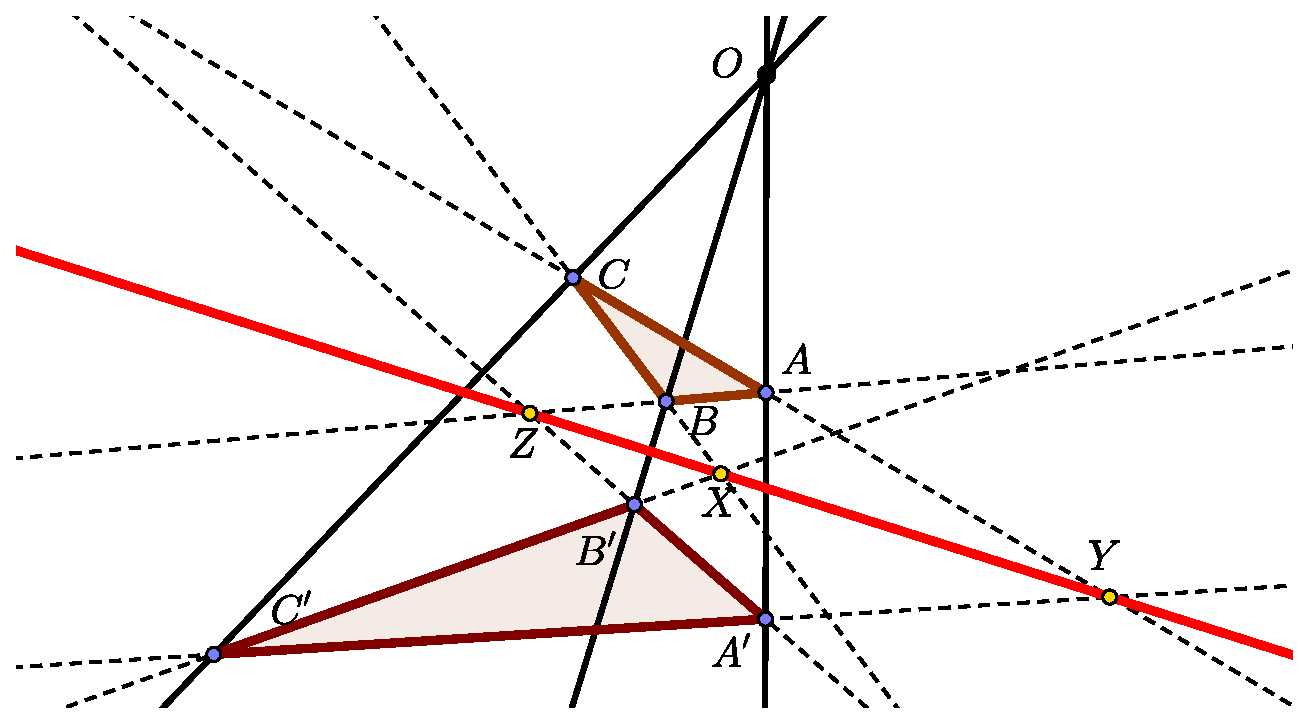
\includegraphics[scale=.45]{Graficos/desargues.eps}
		\caption{Ilustración del Teorema de Desargues.}
		\label{C7_img_desargues}
	\end{figure}
	
\end{theo}
\begin{proof}
	Suponiendo que los triángulos están en perspectiva, demostremos que los puntos $X,Y,Z$ son colineales. Para ello, demostraremos que sus representantes (independientemente de cuales escojamos) son linealmente dependientes.
	
	Antes de comenzar, fijemos notaciones:
	\[\begin{array}{ccc}
	& O=\class{\vec{o}} & \\
	A=\class{\vec{a}}   & B=\class{\vec{b}}   & C=\class{\vec{c}}\\
	A'=\class{\vec{a'}} & B'=\class{\vec{b'}} & C'=\class{\vec{c'}} 
	\end{array}\]
	
	Como los triángulos están en perspectiva, se tiene que los puntos $O,A,A'$ (distintos) están alineados, es decir, tienen representantes coplanarios. Por ende, podremos escribir uno de estos representantes como combinación lineal de los otros. En este caso escribiremos:
	\[\vec{a'}=\lambda \vec{o}+\alpha\vec{a}\]
	Como los puntos son distintos, es claro que $\vec{a'}$ no se podrá escribir como múltiplo de un solo representante, esto significa que ambos coeficientes de la combinación lineal son no nulos, luego, dividiendo por $\lambda$ y renombrando (cometiendo cierto abuso de notación) al representante y a las variables obtenemos que:
	\[\vec{a'}=\vec{o}+\alpha\vec{a}\]
	Repitiendo esta misma jugada con los puntos $O,B,B'$ y $O,C,C'$ obtemos las identidades:
	\[\begin{array}{lr}
	\vec{b'}=\vec{o}+\beta\vec{b} \qquad&\qquad
	\vec{c'}=\vec{o}+\gamma\vec{c}
	\end{array}\]
	Una forma fácil de hallar un representante del punto $Z$ es restar los vectores $\vec{a'}$ y $\vec{b'}$. En efecto:
	\[\vec{a'}-\vec{b'}=\alpha\vec{a}-\beta\vec{b}=:\vec{z}\in\lengen{\vec{a'},\vec{b'}}\cap\lengen{\vec{a},\vec{b}}\stackrel{\eqref{C1_eq_explicitaEngendrados}}{\ra}\class{\vec{z}}\in A'B'\cap AB=:Z\]
	De nuevo, repetimos esta idea para hallar representantes de los puntos $X$ e $Y$, obteniendo:
	\[\begin{array}{lr}
	\vec{y}:=\vec{c'}-\vec{a'}=\gamma\vec{c}-\alpha\vec{a}\qquad&
	\qquad \vec{x}:=\vec{b'}-\vec{c'}=\beta\vec{b}-\gamma\vec{c}
	\end{array}\]
	Veamos que los representantes escogidos de los puntos $X,Y,Z$ son linealmente dependientes, para ello basta con sumarlos. En efecto (compruébese):
	\[\vec{x}+\vec{y}+\vec{z}=0\]
	Lo que concluye la demostración de la primera implicación del teorema.
	
	Recíprocamente, los dioses nos reservan un pequeño presente, que hará valer, aún más si cabe, nuestros conocimientos acerca de dualidad. Resulta que, como ya adelantamos, el teorema de Desargues es un teorema \ti{autodual}. Esto quiere decir que, como ya sabemos, podemos optar por, en lugar de demostrar la otra implicación ``a pelo'', demostrar su dual. Sin embargo, resulta que al dualizar el enunciado de esta segunda implicación, obtenemos el enunciado de la primera (ya demostrada), por lo cual, acabamos de reducir un problema de complejidad desconocida, a una simple trivialidad. Es por esto que se suele decir que el recíproco del teorema de desargues es obvio por dualidad.
	
	La comprobación de que esto es así es un sencillo ejercicio para el cual se recomienda refrescar la sección \ref{C2_principioDualidadProyectiva}.
\end{proof}
Nótese que en la demostración de la primera implicación del teorema no se ha usado para nada la hipótesis de que los puntos se encuentren en el plano proyectivo, esto nos hace ver que dicho fragmento del teorema es válido para dimensión arbitraria (finita). Sin embargo, recordemos que a la hora de comprobar que, efectivamente, el dual del enunciado de la segunda implicación era el enunciado de la primera, esta hipótesis nos fue crucial.

Aunque la demostración que hemos visto del teorema de Desargues no es especialmente enrevesada ni difícil, quizá si puede no ser muy intuitiva y de tener cierta componente de idea feliz, es por esto que veremos otras dos demostraciones del mismo teorema al final del capítulo.
\section{Perspectividades}
\label{C7_Perspectividades}
Comencemos ya con la parte central del capítulo, el estudio de las \ti{perspectividades}. Comencemos por la definición.
\begin{defi}[Perspectividad]
	\label{C7_defi_perspectividad}
	Una homografía $h:l\to l'$, donde $l$ y $l'$ son rectas distintas de $\proy^2$ se dice \ti{perspectividad} si es la restricción a $l$ es la proyección cónica de centro $O(\not\in l\cup l')$ en $l'$. Es decir:
	\[\left.\begin{array}{ccc}\proy^2\setminus{O}&\stackrel{\pi_O}{\to}&l'\\p& \mapsto & Op\cap l'\end{array}\right\}\leadsto h\equiv \pi_O|l\]
\end{defi}
Obsérvese que con la definición \ref{C7_defi_perspectividad} no hemos hecho más que revisitar el viejo ejemplo \ref{C4_exa_fabricaHomografias}.
\begin{figure}[h]
	\centering
	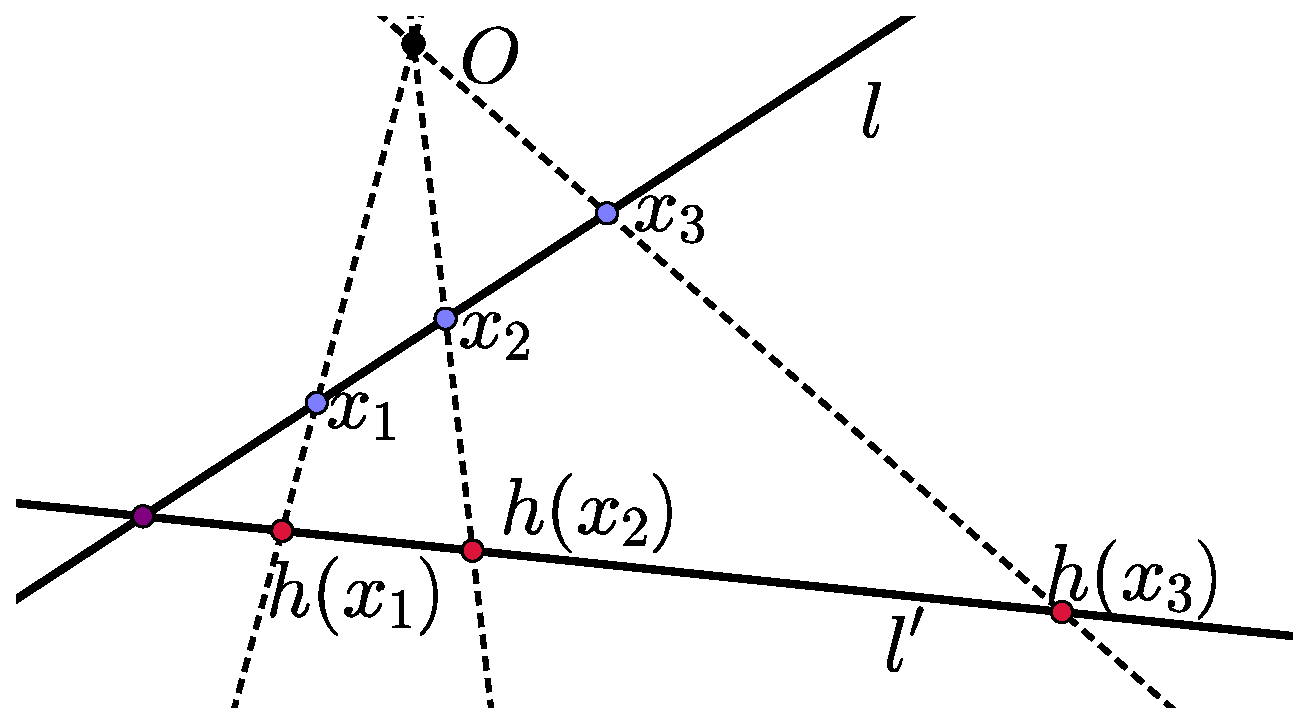
\includegraphics[scale=.3]{Graficos/perspectividad.eps}
	\caption{Ilustración de una Perspectividad.}
	\label{C7_img_perspectividad}
\end{figure}

La comprobación de ser perspectividad parece bastante engorrosa, por ello, los geómetras del mundo se pusieron a trabajar y obtuvieron la siguiente caracterización, que si uno mira la figura \ref{C7_img_perspectividad}, es bastante intuitiva.
\begin{prop}[Caracterización de las Perspectividades]
	\label{C7_prop_caracterizacionPerspectividades}
	Una homografía $h:l\to l'$ es perspectividad si y solo si deja fijo el punto $c:=l\cap l'$.
\end{prop}
\begin{proof}
	Supongamos que la homografía deja fijo el punto $c$. Tomemos dos puntos distintos $P,Q$ de la recta $l$ distintos de $c$. Consideremos asimismo sus imágenes $P'=h(P)$ y $Q'=h(Q)$. Es evidente (por estar en $\proy^2$) que las rectas $PP'$ y $QQ'$ se cortarán en cierto punto $O$. Entonces, resulta que nuestra homografía $h$ coincide con la perspectividad de centro $O$ que va de $l$ a $l'$ en tres puntos distintos; $c, P, Q$. Como vimos en la proposición \ref{C5_prop_homografia3puntos}, que dos homografías de la recta coincidan en tres puntos, implica que estas son iguales, por ende, nuestra homografía $h$ es una perspectividad. El recíproco es obvio.
\end{proof}
La proposición \ref{C7_prop_caracterizacionPerspectividades} nos da una forma bastante cómoda de comprobar que una homografía es una perspectividad.
\subsection{Perspectividades y Dualidad}
Para terminar la sección, tratemos de dar una interpretación dual al concepto de perspectividad.

Como sabemos, los puntos de una recta del plano proyectivo se corresponden, por dualidad canónica, con un haz de rectas con cierta base.

Así pues, la interpretación dual de una homografía $h$ entre dos rectas $l$ y $l'$ será una aplicación $h^*$ entre dos haces de rectas $\haz_A$ y $\haz_B$.

Dicha aplicación enviará cada recta $x^*\in\haz_A$ a otra recta $y^*\in\haz_B$. Donde la recta $x^*$ se corresponde con el punto $x\in l$, y la recta $y^*$ es el dualizado del punto $y=h(x)\in l'$.

Pasemos ahora a dualizar la definición de perspectividad.
\begin{defi}[Perspectividad Dual]
	Una homografía $h^*$ entre dos haces de rectas se dirá \ti{perspectividad} si a cada recta $p^*$ del haz de partida le asigna $\engen{O^*\cap p^*,l'^*}$ donde $O^*$ es una recta que no pertenece a ninguno de los haces.
\end{defi}
\begin{figure}[h]
	\centering
	
\includegraphics[scale=.1]{Graficos/perspectividadDual.eps}
	\caption{Ilustración de una Perspectividad Dual.}
	\label{C7_img_perspectividadDual}
\end{figure}
Hecho esto, podemos dualizar la proposición \ref{C7_prop_caracterizacionPerspectividades}.
\begin{prop}[Caracterización de Perspectividades Dual]
	\label{C7_lem_caracterizacion_persp_dual}
	Una homografía dual $h^*$ entre $\haz_A$ y $\haz_B$ es una perspectividad si y solo si deja fija la recta $AB$.
\end{prop}
\begin{proof}
	Basta comprobar que hemos traducido bien el enunciado de la proposición \ref{C7_prop_caracterizacionPerspectividades}.
\end{proof}
\section{Factorización de Homografías}
\label{C7_factorizacion}
El objetivo de esta sección es poner de manifiesto la utilidad de las perspectividades, probando que cualquier homografía entre rectas del plano puede ser escrita como composición de perspectividades.
\begin{prop}[Primer Teorema de Factorización]
	\label{C7_prop_factorizacion}
	Consideramos $l,l'\subset\proy^2$ rectas distintas y una homografía $h:l\to l'$ entre ambas. Entoces existen dos perspectividades $\pi_1:l\to\bar{l}$ y $\pi_2:\bar{l}\to l'$ tales que verifican:
	\[\pi_2\circ\pi_1=h\]
\end{prop}
\begin{proof}
	Como $h$ queda determinada por las imágenes de tres puntos distintos, consideramos los puntos $P,Q,R\in l$ (distintos) y sus respectivas imágenes por $h$, a las que denotaremos $P',Q'$ y $R'$. Nuestra estrategia será construir una perspectividad que lleve $P,Q$ y $R$ a ciertos puntos de una recta intermedia $\bar{l}$. A continuación construiremos otra perspectividad que rescate a los transformados de $P,Q$ y $R$ por la primera perspectividad y los lleve a donde los llevaba $h$.
	
	Consideremos dos puntos $V,V'$ sobre la recta $RR'$ distintos de $R$ y $R'$ (que serán los centros de nuestras perspectividades). Consideramos ahora la recta:
	\[\bar{l}=\engen{VQ\cap V'Q', VP\cap V'P'}\]
	Si tomamos las perspectividades:
	\[\begin{array}{cc}
	\pi_1=\pi_V:l\to\bar{l} \qquad&\qquad \pi_2=\pi_{V'}:\bar{l}\to l
	\end{array}\]
	Entonces resulta que $\pi_2\circ\pi_1$ coincide con $h$ en tres puntos distintos ($P,Q$ y $R$), por ende son la misma homografía.
\end{proof}
La demostración del teorema \ref{C7_prop_factorizacion} puede parecer poco intuitiva, sin embargo, geométricamente es muy visual, es por ello que se recomienda visitar la figura \ref{C7_img_factorizacion}.
\begin{figure}[h]
	\centering
	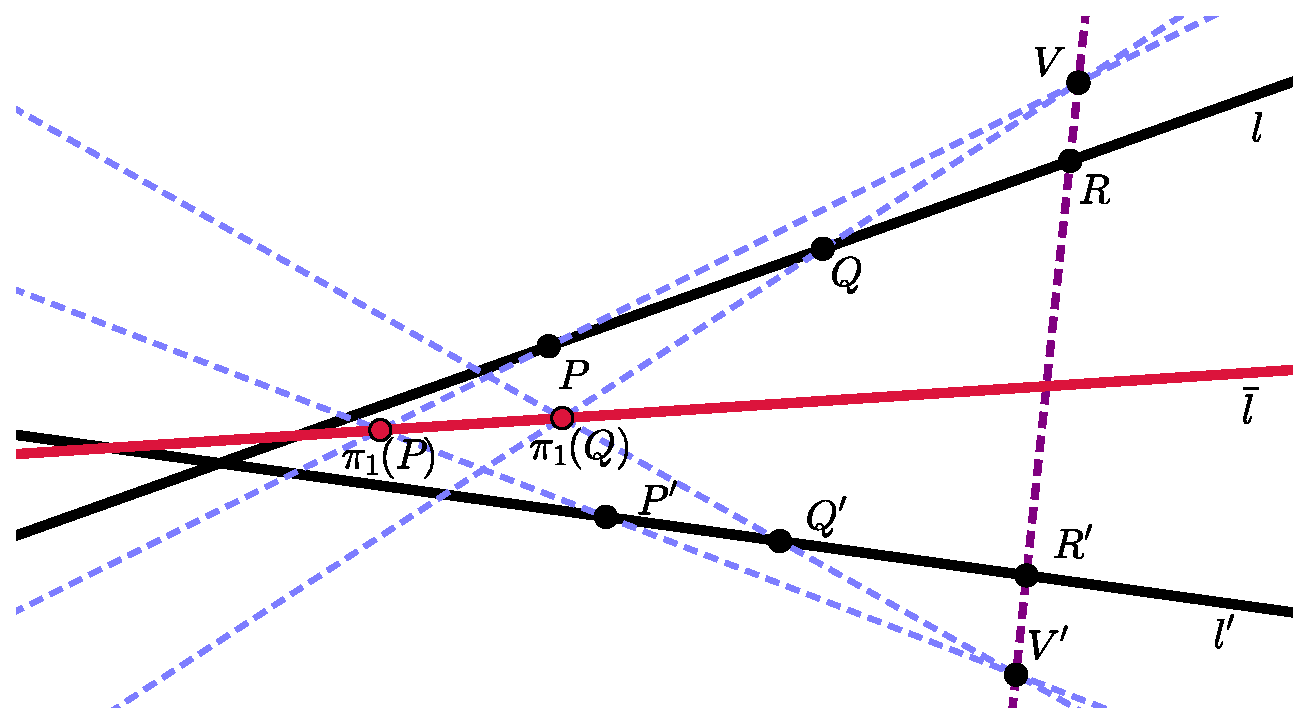
\includegraphics[scale=.4]{Graficos/factorizacion.eps}
	\caption{Ilustración de la prueba de la proposición \ref{C7_prop_factorizacion}.}
	\label{C7_img_factorizacion}
\end{figure}
\begin{obs}[No Unicidad de la Factorización]
	Es importante observar que la factorización de una homografía como composición de perspectividades no es, ni mucho menos, única. Basta tomar otros puntos $V$ y $V'$ como centros de las perspectividades.
\end{obs}
\begin{obs}[Homografías ``Automórficas'']
	\label{C7_obs_automorficas}
	Nótese que la demostración de la proposición \ref{C7_prop_factorizacion} hace uso de que las rectas $l$ y $l'$ son distintas. Esto quiere decir que, por ahora, no podemos decir que una homografía de una recta en sí misma pueda ser factorizada como composición de perspectividades. Dicho pedantemente, no sabemos si el grupo proyectivo o \ti{grupo de homografías} de una recta está generado por perspectividades.
\end{obs}
Vemos a continuación una consecuencia bastante importante (pues resulve el problema planteado en la observación \ref{C7_obs_automorficas}) de la proposición \ref{C7_prop_factorizacion}.
\begin{cor}[Segundo Teorema de Factorización]
	Una homografía $h:l\to l$ (siendo $l$ una recta de $\proy^2$) puede generarse como composición de, a lo sumo, tres perspectividades.
\end{cor}
\begin{proof}
	Supongamos que la homografía $h$ en cuestión viene definida por los siguientes tres puntos distintos de $l$ y sus imágenes
	\[\begin{array}{ccc}
	P\mapsto \overline{P}\qquad&\qquad
	Q\mapsto \overline{Q}\qquad&\qquad
	R\mapsto \overline{R}
	\end{array}\]
	Consideremos $l'$ cualquier recta distinta de $l$. Tomemos asimismo un punto $V$ que no se encuentre ni en $l$ ni en $l'$. Planteamos la perspectividad $\pi_V$ de centro $V$, que nace en $l$ y muere en $l'$. Para poder trabajar cómodamente caractericémosla por sus imágenes de los tres puntos anteriores $P,Q$ y $R$. A dichas imágenes las llamaremos $P',Q'$ y $R'$ respectivamente.
	
	\begin{center}
		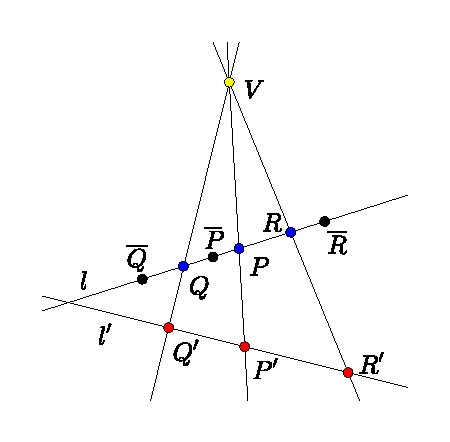
\includegraphics[scale=.9]{Graficos/Desargues/perspectividad}
	\end{center}
	
	Ahora tomemos la homografía $h':l'\to l$ definida por las condiciones
	\[\begin{array}{ccc}
	P'\mapsto \overline{P}\qquad&\qquad
	Q'\mapsto \overline{Q}\qquad&\qquad
	R'\mapsto \overline{R}
	\end{array}\]
	la cual es única.
	
	Es claro que $h=h'\circ\pi_V$, pero como $h'$ es homografía, basta aplicar la proposición \ref{C7_prop_factorizacion} para obtener que:
	\[h=\pi_1\circ\pi_2\circ\pi_V\]
	Como todas son perspectividades, hemos terminado.
\end{proof}

\begin{obs}
	Este corolario nos proporciona una demostración alternativa de que la construcción del cuadrilátero completo produce cuaternas armónicas. En efecto, consideremos el cuadrilátero completo formado por los puntos $A,B,C,D$, el cual se muestra en la siguiente figura. 
	\begin{center}
		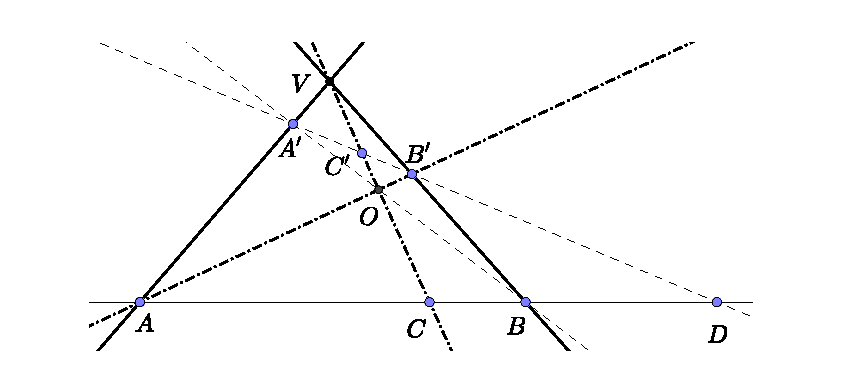
\includegraphics[scale=.9]{Graficos/Desargues/cuadrilatero}
	\end{center}
	Consideramos la perspectividad $\pi_O$ de centro $O$, que transforma los puntos $A,B,C,D$ en $B',A',C',D$ respectivamente, y la pespectividad $\pi_V$ de centro $V$, que transforma los puntos $A',B',C',D$ en $A,B,C,D$, respectivamente. Al ser homografías se tiene que
	\[\{A,B;C,D\}=\{B',A';C',D\}=\{B,A;C,D\}\]
	Por las propiedades de la razón doble (sección~\ref{C5_sec_simetrias}) si $\{A,B;C,D\}=\lambda$, entonces $\{B,A;C,D\}=\frac{1}{\lambda}$. Por tanto, necesariamente, $\lambda=1$ o $-1$.
	
	Dado que son puntos distintos, podemos escoger como referencia los primeros tres $\mf{R}=\{A,B;C\}$. Esto nos daría, como ya vimos, que $\lambda$ es la coordenada de $D$ respecto a $\mf{R}$. Si $\lambda=1$, entonces $D=C$, lo cual no ocurre pues los hemos escogido distintos. Por tanto, se concluye que 
	\[\{A,B;C,D\}=-1\]
\end{obs}
\section{Teorema del Eje}
\label{C7_Eje}
Para finalizar el capítulo enunciemos y demostremos el llamado ``Teorema del Eje''.

El enunciado del siguiente teorema puede resultar algo confuso a primera vista, sin embargo, un breve vistazo a las figuras que se muestran a continuación debería despejar todas las dudas.
\begin{theo}[Teorema del Eje]
	\label{C7_teo_eje}
	Sean dos rectas $l,l'\subset\proy^2$ distintas y una homografía $h:l\to l'$. Se cumple que el conjunto:
	\[e:=\{x\in\proy^2\tq x=Ph(Q)\cap Qh(P)\tq P,Q\in l\}\]
	es una recta. A esta la llamaremos \ti{eje} de la homografía $h$. 
\end{theo}
\begin{proof}
	Procedamos a la demostración del resultado mediante una distinción de casos. En primer lugar se tratará el caso en el que $h$ es una perspectividad, para después pasar al caso general.\\
	
	\underline{Caso 1}: Suponiendo que $h$ es una perspectividad de centro $V$, consideramos los puntos $P,Q\in l$ arbitrarios y sus respectivas imágenes $P'Q'\in l'$. Asimismo consideramos el punto $X=PQ'\cap P'Q$. Veamos que $e=OX$, donde $O=l\cap l'$.
	
	Como se observa en la imagen los puntos $V,Q,R,Q'$ forman una cuaterna armónica, ya que la construcción geométrica mostrada no es otra que el cuadrilátero completo. Por tanto, como vimos, $\{l,l',OX,OV\}=-1$. Además, recordemos que (como ocurría con los puntos) dadas tres rectas la construcción del cuadrilátero completo nos proporciona siempre la misma cuarta recta, con la cual se forma una cuaterna armónica. Como las rectas $l,l',OV$ son fijas, esto obliga a que la recta $OX$ sea fija. Esto prueba que la recta $OX$ esta formada por puntos de la forma $Ph(Q)\cap Qh(P)$. Es decir, es el eje de la perspectividad.
	\begin{center}
		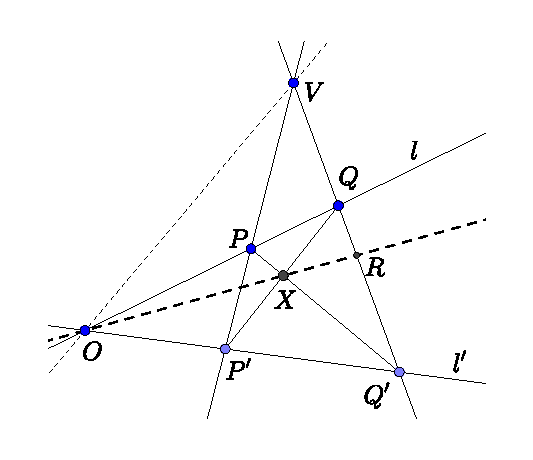
\includegraphics[scale=.9]{Graficos/TeoremaDelEje/TeoremaDelEjeCaso1}
	\end{center}
	\underline{Caso 2}: Supongamos que $h$ no es una perspectividad. Entonces, no deja fijo $l\cap l'=O$. Podemos considerar, por tanto, los puntos $h(O)=V\in l'$ y $
	h^{-1}(O)=U\in l$, ambos distintos de $O$. Veamos que $UV$ es el eje de la homografía. 
	
	Para ello, dados dos puntos $P,Q\in l$ arbitrarios y sus imágenes, que denotaremos por $P',Q'\in l'$, basta comprobar que $X=PQ'\cap P'Q\in UV$.
	\begin{center}
		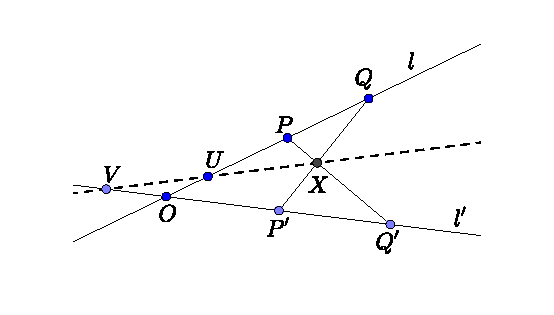
\includegraphics[scale=.9]{Graficos/TeoremaDelEje/TeoremaDelEjeCaso2}
	\end{center}
	Si demostrásemos que existe una homografía $g$ tal que
	\[\begin{array}{cccc}
	g:&l&\rightarrow &l'\\
	&P&\rightarrow&Q'\\
	&Q&\rightarrow&P'\\
	&U&\rightarrow&V\\
	&O&\rightarrow&O
	\end{array}\]
	entonces será una perspectividad por dejar fijo el punto $O=l\cap l'$. El centro de $g$ tendrá que pertenecer a las rectas $PQ',QP'$ y $UV$. Dado que las rectas $PQ'$ y $QP'$ se cortan en el punto $X$, este es el único punto que pertenece a ambas. Por tanto, necesariamente este debe ser el centro, y por ello $X\in UV$, que es lo que buscábamos.
	
	Veamos que la homografía $g$ existe. Para ello, comprobemos que se preserva la razón doble. Al ser $h$ homografía y por simetría se tiene que
	\begin{multline}
		\{P,Q;U,O\}=\{h(P),h(Q);h(U),h(O)\}=\{P',Q';O,V\}=\{Q',P';V,O\}
	\end{multline}
	Una vez que esto queda comprobado, por el Teorema~\ref{C5_teo_hom4puntos_sii_razondoble} existe la homografía $g$.
\end{proof}

\begin{obs}[Teorema de Pappus]
	Una consecuencia del Teorema del Eje es el Teorema de Pappus. Recordemos el enunciado del Teorema de Pappus.
	
	\textit{Sean $r$ y $r'$ dos rectas diferentes de $\proy(E)$. Entonces, para cualesquiera seis puntos distintos $A,B,C\in r$ y $A',B',C'\in r'$, los puntos
	\begin{equation*}
		X=AB'\cap A'B \ ; \qquad Y=AC'\cap A'C \ ; \qquad Z=BC'\cap B'C
	\end{equation*}
	están alineados.}

	En efecto, existe una única homografía de $r$ en $r'$ que transforma los puntos $A,B,C$ en los puntos $A',B',C'$. Aplicando el Teorema del Eje es inmediato que $X,Y,Z$ están alineados.
\end{obs}

\begin{obs}
	Dada una homografía $h:l\rightarrow l'$, donde $l$ y $l'$ son dos rectas distintas, la imagen por $h$ de cualquier punto $X\in l$ puede construirse usando el eje de la homografía. En efecto, si conocemos otro punto $P$, su imagen $h(P)$ y el eje de la homografía $eje$, como sabemos que $Ph(X)\cap h(P)X$ está en el eje y conocemos $XP'\cap eje$, podemos hallar $h(X)$.
	\begin{center}
		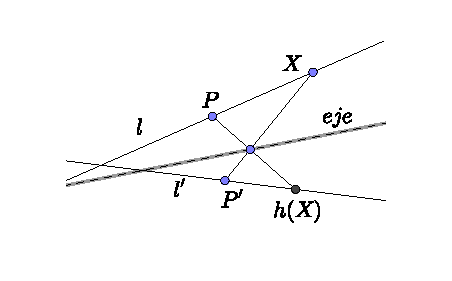
\includegraphics[scale=1]{Graficos/TeoremaDelEje/DeterminacionImagenHom}
	\end{center} 
\end{obs}
\section{Otras Demostraciones del Teorema de Desargues}
A continuación, ofrecemos una demostración alternativa del Teorema de Desargues. Dado que, como vimos, una de las implicaciones es la dual de la otra, solo haremos la demostración de la condición suficiente.
\begin{theo}[Teorema de Desargues]
	Dados dos triángulos en el plano proyectivo $ABC$, $A'B'C'$ con vértices distintos. Consideremos los puntos:
	\[\begin{array}{c}
	Z=AB\cap A'B'\\
	Y=AC\cap A'C'\\
	X=CB\cap C'B'
	\end{array}\]
	Los tríangulos están en perspectiva si y solo si $X,Y,Z$ son colineales.
	\begin{center}
		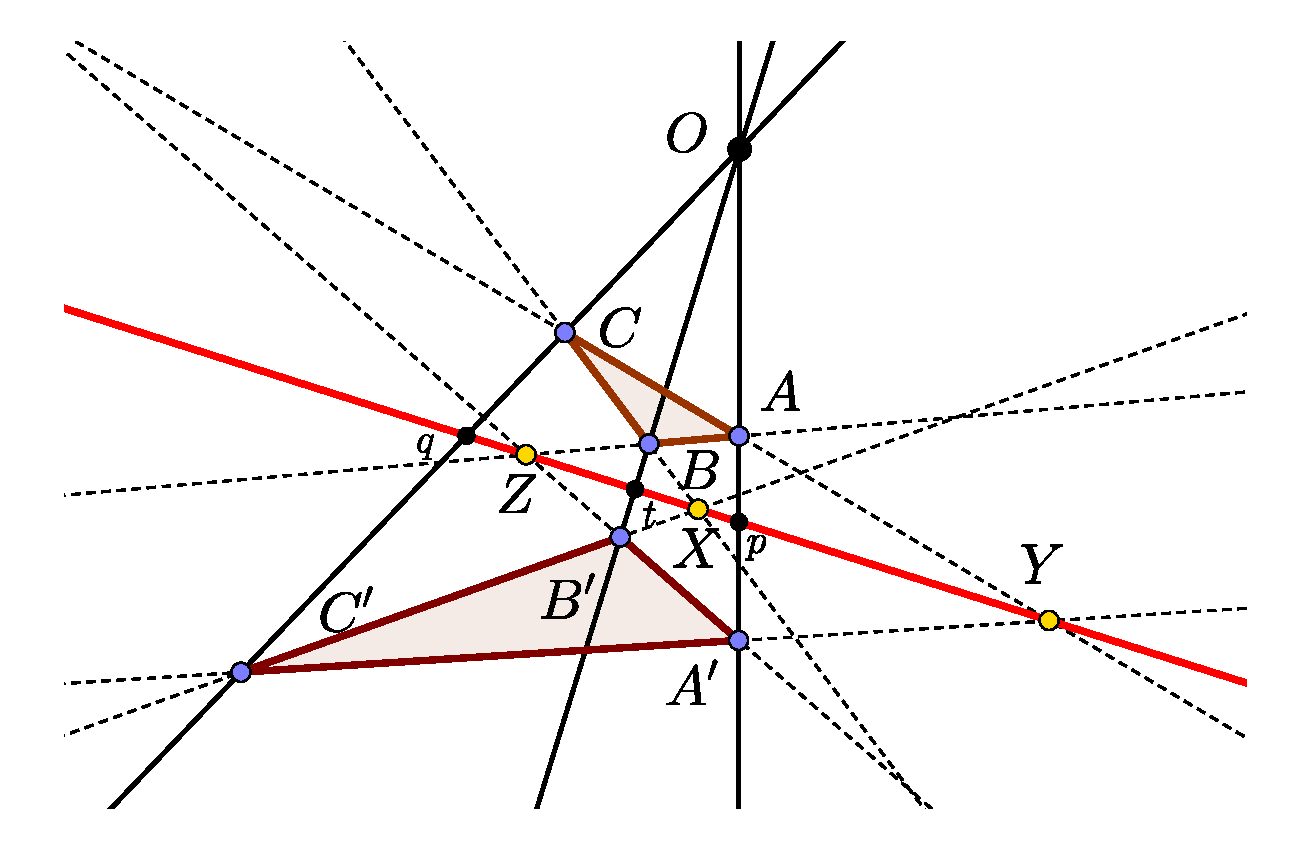
\includegraphics[scale=.45]{Graficos/Desargues/desargues2}
	\end{center}
\end{theo}
\begin{proof}
	Sean las rectas $a=AA',b=BB'$ y $c=CC'$, consideremos la perspectividad de centro $Z$
	\[\pi_Z:a\rightarrow b,\]
	la perspectividad de centro $X$
	\[\pi_X:b\rightarrow c\]
	y la perspectividad de centro $Y$
	\[\pi_Y:a\rightarrow c\]
	Es seguro que todas son perspectividades, ya que dejan fijo el punto $O=a\cap b=b\cap c=a\cap c$.
	
	La composición de las dos primeras es la aplicación proyectiva
	\[\pi=\pi_X\circ \pi_Z:a\rightarrow c\]
	Dado que $\pi(O)=\pi_X(\pi_Z(O))=O=a\cap c$ se concluye que también es una perspectividad.
	
	Veamos que punto es el centro de $\pi$. Como $\pi(A)=\pi_X(\pi_Z(A))=C$, $\pi(A')=\pi_X(\pi_Z(A'))=C'$ y el centro viene dado por $A\pi(A)\cap A'\pi(C')$, el centro de la perspectividad no es otro que el punto $AC\cap A'C'=Y$. Por tanto, $\pi=\pi_Y$.
	
	Tomemos ahora los puntos $q=ZX\cap c,p=ZX\cap a$ y $t=ZX\cap b$. Se tiene que
	\[\pi(p)=\pi_X(\pi_Z(p))=\pi_X(t)=q\]
	Recordemos que, por otro lado, habíamos visto que $\pi=\pi_Y$. Por tanto, $\pi_Y(p)=q$. Esto implica que los puntos $Y,p$ y $q$ están alineados. Como, por construcción de $p$ y $q$, los puntos $X,Z,p,q$ también están alineados, se tiene que $Y,X$ y $Z$ están alineados, concluyendo así nuestra demostración.
\end{proof}
	\part{Variedades cuadráticas. Conexiones con otras geometrías}
	\chapter{Cónicas y Cuádricas}
\label{C8}
A lo largo del capítulo $\ref{C2}$ estudiamos con detalle el conjunto de puntos que eran anulados por unas aplicaciones muy concretas, a las que llamamos \ti{formas lineales}.

En este capítulo haremos algo parecido, dando un pequeño paso adelante, pues estudiaremos las interesantes propiedades del conjunto de ceros de las llamadas \ti{formas cuadráticas}.

A no ser que establezcamos explícitamente lo contrario, a lo largo de este capítulo trabajaremos con el cuerpo de los números complejos y el plano proyectivo complejo $\proy(\C^3)=\proy^2$. 

Esto es debido a que, como se verá inmediatamente, trabajaremos con polinomios, siendonos muy útil la posibilidad de aplicar el Teorema Fundamental del Álgebra y sus consecuencias.

El capítulo comienza con una fuerte introducción teórica acerca de formas bilineales y cuadráticas (muy susceptible de haber sido olvidada), e indispensable para comprender en profundidad los resultados centrales del capítulo (razón por la cual se ha decidido incluirla aquí y no en un apéndice dedicado).

\section{Conceptos Previos. Formas Bilineales y Cuadráticas}
A lo largo de este capítulo estudiaremos las llamadas \ti{cuádricas}. Para poder definir de forma rigurosa este concepto, necesitamos recordar (o introducir) algunas nociones importantes más propias del álgebra lineal.
\subsection{Formas Bilineales}
Sea $E$ un espacio vectorial arbitrario de dimensión $n$. (Normalmente trabajaremos con $\C^n$).
\begin{defi}[Forma Bilineal]
	\label{C8_def_formaBilineal}
	Llamamos \ti{formas bilineales} a las aplicaciones de la forma \[\begin{array}{cc}f:&E\times E\to\K\\
	& (u,v)\mapsto f(u,v)\end{array}\]
	Donde $f$ es ``lineal respecto de ambas componentes''. Es decir, dado un par $(u,v)\in E\times E$, se verifica:
	\begin{enumerate}
		\item Linealidad respecto de la primera componente: \[f(\alpha u_1,\beta u_2, v)=\alpha f(u_1,v)+\beta f(u_2,v)\]
		\item Linealidad respecto de la segunda componente:
		\[f(u,\alpha v_1 +\beta v_2)=\alpha f(u,v_1)+\beta f(u,v_2)\]
	\end{enumerate}
\end{defi}
En este punto es fructífero recordar que una aplicación lineal queda totalmente determinada por las imágenes de los vectores de una base de su espacio vectorial de partida.

Este resultado daba lugar a la idea caracterizar cada aplicación lineal $f$ por una matriz, a la que llamábamos \ti{matriz asociada a $f$}.

Tratemos de trasladar esta idea al ámbito de las formas bilineales.
\subsubsection{Matriz Asociada a una Forma Bilineal}
Fijemos una base $\mc{B}:=\{e_1,\dots,e_n\}$ del espacio vectorial $E$.

Veamos cuál es la imagen del par $(u,v)$ por una forma bilineal arbitraria $f$. Para ello, escribiremos los vectores $u$ y $v$ como combinación lineal de la base $\mc{B}$ y aplicaremos las propiedades de bilinealidad (definición \ref{C8_def_formaBilineal})
\[f(u,v)=f\left(\sum_{i=1}^{n}a_ie_i,\sum_{j=1}^{n}b_je_j\right)=\sum_{i=1}^{n}a_i\left(\sum_{j=1}^{n}f(e_i,e_j)b_j\right)\]
Podemos interpretar el interior del paréntesis como un producto de matrices (matriz fila por matriz columna). Haciendo esto obtenemos la siguiente expresión, más compacta (los corchetes son sólo notacionales).
\[f(u,v)=\sum_{i=1}^{n}a_i\left[\begin{pmatrix}
f(e_i, e_1) & 
\cdots &
f(e_i, e_n)
\end{pmatrix}\begin{pmatrix}
b_1 & \cdots & b_n
\end{pmatrix}^t\right]\]
Por comodidad notacional, a la matriz columna que representa las coordenadas de $v$ respecto de $\mc{B}$ será denotado por $Y$. Análogamente, llamaremos $X$ a la matriz columna que representará las coordenadas de $u$ respecto de $\mc{B}$.

Con esta notación (y reordenando por conveniencia los corchetes) nos queda:
\[f(u,v)=\left[\sum_{i=1}^{n}a_i\begin{pmatrix}
f(e_i, e_1) & 
\cdots &
f(e_i, e_n)
\end{pmatrix}\right]Y\]
Como hicimos antes, podemos interpretar la suma anterior de manera matricial (las comprobaciones de dejan al lector)
\[f(u,v)=\begin{pmatrix}
a_1 & \cdots & a_n
\end{pmatrix}\begin{pmatrix}
f(e_1, e_1) & \cdots & f(e_1,e_n)\\
\vdots & \ddots & \vdots\\
f(e_n,e_1) & \cdots & f(e_n,e_n)
\end{pmatrix}Y\]
Usando nuestras notaciones habituales y denotando por $M$ a la matriz cuadrada obtenemos:
\begin{equation}
\label{C8_eq_ecuacionMatricialBilineal}
f(u,v)=X^tMY
\end{equation}
A la matriz $M$ de la ecuación \eqref{C8_eq_ecuacionMatricialBilineal} se la llama \ti{matriz asociada a la forma bilineal $f$}.

Se ve inmediatamente por la ecuación \eqref{C8_eq_ecuacionMatricialBilineal} que si dos formas bilineales $f$ y $g$ tienen a $M$ por matriz asociada, estas son necesariamente la misma aplicación.

Esto quiere decir que una forma bilineal $f$ queda totalmente determinada por su matriz asociada, es decir, por las imágenes de los pares de vectores $(e_i,e_j)$ donde $i,j\in\{1,\dots,n\}$.

\begin{obs}[Lema de la Correspondencia]
	\label{C8_obs_correspondencia}
	Es claro que a lo largo de este proceso hemos probado que, \tb{fijada una base} $\mc{B}$ de $E$, toda forma bilineal $f$ está asociada a una única matriz $M$.
	
	Además, el recíproco también es cierto, fijada una base, toda matriz cuadrada es la asociada de una única forma bilineal.
	
	La prueba de este hecho consiste símplemente en definir una forma bilineal $f$ de manera que la imagen de un par de la forma $(e_i,e_j)$ se corresponda con el coeficiente $a_{ij}$ de la matriz dada. 
\end{obs}
\subsection{Formas Cuadráticas}
Introducidos ya los aspectos generales de las formas bilineales, pasemos a definir la noción de \ti{forma cuadrática}.
\begin{defi}[Forma Cuadrática]
	Una aplicación $\Phi$ se dice \ti{forma cuadrática} si es de la forma:
	\[\begin{array}{cc}
	\Phi: & E\to \K\\
	& x\mapsto f(x,x)
	\end{array}\]
	donde $f$ es una forma bilineal.
\end{defi}
Es claro que, fijada una base, las formas cuadráticas cumplen la siguiente ecuación matricial:
\begin{equation}
\label{C8_eq_ecuacionCuadraticas}
	\Phi(x)=X^tMX
\end{equation}
Una propiedad agridulce de las formas cuadráticas es que pueden estar asociadas a varias formas bilineales, tal y como muestra el siguiente ejemplo.
\begin{exa}[Varias Formas Bilineales Asociadas]
	Sean las formas bilineales de matrices asociadas:
	\[f\equiv\begin{pmatrix}
	1 & 4\\
	2 & 2
	\end{pmatrix}\qquad g\equiv\begin{pmatrix}
	1 & 3\\
	3 & 2
	\end{pmatrix}\]
	Comprobemos que ambas formas bilineales tienen la misma forma cuadrática asociada.
	\[\Phi_f(x)=\begin{pmatrix}
	x_1 & x_2
	\end{pmatrix}\begin{pmatrix}
	1 & 4\\
	2 & 2
	\end{pmatrix}\begin{pmatrix}
	x_1\\
	x_2
	\end{pmatrix}=x_1^2+6x_1x_2+2x_2^2\]
	\[\Phi_g(x)=\begin{pmatrix}
	x_1 & x_2
	\end{pmatrix}\begin{pmatrix}
	1 & 3\\
	3 & 2
	\end{pmatrix}\begin{pmatrix}
	x_1\\
	x_2
	\end{pmatrix}=x_1^2+6x_1x_2+2x_2^2\]
\end{exa}
Decimos que esta propiedad es ``agridulce'', porque por una parte es más bonito que haya una correspondencia ``limpia'' entre formas bilineales y formas cuadrátricas. Sin embargo, las propiedades que vienen a continuación compensan con creces esto último. Antes de poder presentarlas, necesitamos una pequeña definición.
\begin{defi}[Formas Bilineales Simétricas y Antisimétricas]
	\label{C8_def_simetricaAntisimetrica}
	Decimos que una forma bilineal $f$ es \ti{simétrica} si su matriz asociada es simétrica. Análogamente, $f$ será \ti{antisimétrica} (o \ti{alternada}) si su matriz asociada es antisimétrica.
\end{defi}
Nótese que en la definición \ref{C8_def_simetricaAntisimetrica} hablamos de la matriz asociada a una forma bilineal como si solo hubiera una y no muchas (una por cada base fijada).

De esta forma, en primera instancia, uno podría pensar que es posible que hubiera dos bases; $\mc{B}$ y $\overline{\mc{B}}$, de manera que la matriz asociada a cierta forma bilineal $f$ fuera simétrica respecto de la base $\mc{B}$ y antisimétrica respecto de $\overline{\mc{B}}$.

Los siguientes lemas demuestran que esto es imposible. Más aún, veremos que  si la matriz asociada a una forma bilineal $f$ es simétrica respecto de una base $\mc{B}$, lo será también respecto de cualquier otra base $\overline{\mc{B}}$.

De esta forma, podemos decir que la simetría o antisimetría de una forma bilineal es una propiedad intrínseca de la aplicación y no del modo en que la miramos.
\begin{lem}[Caracterización de las Formas Bilineales Simétricas]
	\label{C8_lem_caracterizacionSimetria}
	$f$ es una forma bilineal simétrica si y solo si se verifica que \[f(x,y)=f(y,x)\]
\end{lem}
\begin{proof}
	Si $f$ es una forma bilineal simétrica entonces \[f(x,y)=X^tMY=(X^tMY)^t=Y^tM^tX=Y^tMX=f(y,x)\]
	Recíprocamente, si $f(x,y)=f(y,x)$ es claro que \[a_{ij}:=f(e_i,e_j)=f(e_j,e_i)=:a_{ji}\]
	Que es la definición de ser una matriz simétrica.
\end{proof}
\begin{lem}[Caracterización de las Formas Bilineales Antisimétricas]
	$f$ es una forma bilineal simétrica si y solo si se verifica que \[f(x,y)=-f(y,x)\]
\end{lem}
\begin{proof}
	Se deja como ejercicio al lector. Es totalmente análoga a la del lema \ref{C8_lem_caracterizacionSimetria}. 
\end{proof}
Demostrados los lemas anteriores, que quizá nos hayan roto un poco el discurrir de la teoría, veamos cuál es su verdadera utilidad.

Los siguientes resultados, elementales, pero cruciales, nos hacen ver que, de alguna manera, hay una forma bilineal canónica asociada a cada forma cuadrática. 
\begin{lem}[Formas Cuadráticas Idénticamente Nulas]
	\label{C8_lem_antisimetricaNula}
	Si $\Phi$ es una forma cuadrática asociada a una forma bilineal antisimétrica, entonces $\Phi$ es idénticamente nula.
\end{lem}
\begin{proof}
	Por la ecuación \eqref{C8_eq_ecuacionCuadraticas} sabemos que:
	\[\Phi(x)=X^tMX\in\K\]
	Tenemos que tratar de aplicar en algún sitio que la matriz $M$ es antisimétrica, para lo cual, lo ideal es trasponer en angún lugar.
	
	Como $X^tMX$ es un simple número, coincide con su traspuesto, lo cual nos arroja:
	\[\Phi(x)=X^tMX=(X^tMX)^t=X^tM^tX=-X^tMX=-\Phi(x)\]
	Por ende, $2\Phi(x)=0$, de lo que se desprende que $\Phi(x)=0$ para cualquier $x\in E$.
\end{proof}
\begin{lem}
	\label{C8_lem_descomposicion}
	Sea $M$ una matriz cuadrada, admite una descomposición como suma de una matriz simétrica y otra antisimétrica.
	\[M= M_s+M_a\]
	Además
	\[\begin{array}{cc}
	M_s=\frac{1}{2}(M+M^t)\qquad &\qquad M_a=\frac{1}{2}(M-M^t)
	\end{array}\]
	En términos de formas bilineales; toda forma bilineal puede descomponerse como suma de una forma bilineal simétrica y una forma bilineal antisimétrica.
\end{lem}
\begin{proof}
	Se deja como ejercicio al lector (es una comprobación trivial).
\end{proof}
\begin{obs}[Redundancia de la Parte Antisimétrica]
	De los lemas \ref{C8_lem_antisimetricaNula} y \ref{C8_lem_descomposicion} se deduce que la parte antisimétrica de una forma bilineal asociada a una forma cuadrática sólo nos aporta ruido y confusión.
	
	En efecto, dada una forma cuadrática $\Phi$ tenemos que
	\begin{multline}\Phi(x)=X^tMX=X^t(M_s+M_a)X=\\=(X^tM_s+X^tM_a)X=X^tM_sX+X^tM_aX=X^tM_sX\end{multline}
	Esto constituye una fábrica de formas bilineales asociadas a una misma forma cuadrática.
	
	El hecho de que esto sea siquiera posible nos lleva a la idea de que sería recomendable deshacernos de esa dichosa parte antisimétrica (ya que es más inútil que un cubo de trapo).
\end{obs}
Si combinamos los lemas \ref{C8_lem_antisimetricaNula} y \ref{C8_lem_descomposicion} obtenemos que, tal y como nos asegura el siguiente resultado, una forma cuadrática está asociada a una única forma bilineal simétrica.
\begin{prop}[Lema de la Correspondencia]
	Dada una forma cuadrática $\Phi$, esta está asociada a una única forma bilineal simétrica $f_p$.
	
	A dicha forma bilineal se le llama ``\ti{forma polar}'' de $\Phi$.
\end{prop}
\begin{proof}
	Es una comprobación inmediata ver que se cumple
	\[\Phi(x+y)=f(x,y)+f(y,x)+\Phi(x)+\Phi(y)\]
	Si $f$ es simétrica se cumple que
	\[f(x,y)=\frac{1}{2}\left(\Phi(x+y)-\Phi(x)-\Phi(y)\right)\]
	Por lo que no solo hemos demostrado la unicidad, sino que también hemos obtenido una expresión explícita de la misma.
\end{proof}
Si esta demostración le ha dejado frío al lector (porque ser chapucera y poco intuitiva), que no se alarme, veremos una múcho más útil y elegante en secciones posteriores. (Ver proposición \ref{C8_prop_Hessiana}).
\subsubsection{Matriz Asociada a una Forma Cuadrática}
Podemos definir (por decreto) el concepto de \ti{matriz asociada a una forma cuadrática} $\Phi$ como la matriz asociada a su forma polar.

Pongamos un ejemplo (muy importante en nuestro contexto) para que estos conceptos se arraiguen más.
\begin{exa}[Forma Cuadrática de Dimensión $3$]
	\label{C8_exa_3forma}
	Como sabemos, fijada una base $\mc{B}$, las formas cuadráticas verifican la ecuación matricial
	\[\Phi(\vec{x})=X^tMX\]
	donde consideramos que $M$ es la matriz (simétrica) asociada a la forma cuadrática. En el caso de estar en un espacio vectorial de tres dimensiones tendremos algo del estilo
	\[\Phi(\vec{x})=\begin{pmatrix}
	x & y & z
	\end{pmatrix}\begin{pmatrix}
	a & h & g\\
	h & b & f\\
	g & f & c
	\end{pmatrix}\begin{pmatrix}
	x\\
	y\\
	z
	\end{pmatrix}\]
	Si desarrollamos esto obtenemos la siguiente expresión (que nos será muy familiar de ahora en adelante)
	\begin{equation}
	\label{C8_eq_polinomio}
	\Phi(\vec{x})=ax^2+by^2+cz^2+2fyz+2gzx+2hxy\end{equation}
\end{exa}
Veamos a continuación un sencillo truco memorístico que nos ayudará a obtener sin pensar la matriz asociada a una forma cuadrática sobre un espacio vectorial de dimensión $3$. 
\begin{obs}[Regla Mnemotécnica]
	\label{C8_obs_mnemotecnica}
	Tengamos siempre en mente que (fijemos la base que fijemos) una forma cuadrática de dimensión $3$ tendrá una expresión analítica como la de la ecuación \eqref{C8_eq_polinomio}, donde $x,y,z$ son las coordenadas del vector $\vec{x}$ respecto de la base fijada.
	
	Lo primero que tenemos que tener en cuenta es que la matriz asociada es una matriz simétrica, por lo que únicamente tenemos que calcular el triángulo superior y la diagonal.
	
	En la diagonal de la matriz irán los coeficientes asociados a monomios con variables al cuadrado (por orden, $x^2$, $y^2$ y $z^2$ respectivamente).
	
	Para rellenar el triángulo superior (y por tanto el inferior, por simetría) basta con recorrer dicho triángulo desde su vértice inferior en sentido antihorario y colocar allí los coeficientes asociados a los monomios de variables $yz$, $xz$ y $xy$ respectivamente. (Ver ejemplo \ref{C8_exa_3forma}).
	
	Este truco tiene realmente poca importancia, ya que aprenderemos a calcular esta matriz una forma bastante mecánica. (Ver proposición \ref{C8_prop_Hessiana}).
\end{obs}
 
\subsubsection{Formas Cuadráticas y Polinomios}
Hagamos notar que la expresión analítica de una forma cuadrática sobre un espacio $n$--dimensional siempre será un polinomio en $n$ variables compuesto únicamente por monomios de grado $2$. Expliquemos el significado de este trabalenguas.

\tb{Fijada una base} $\mc{B}$ de $E$, podemos ver cualquier forma cuadrática $\Phi$ como una aplicación \[\widetilde{\Phi_{\mc{B}}}:\K^n\to\K\]
Queremos demostrar que la aplicación $\widetilde{\Phi_{\mc{B}}}$ es siempre un polinomio. Uno muy concreto de hecho.

Comencemos nuestra demostración con algunas definiciones elementales.
\begin{defi}[Monomio]
	Se donomina \ti{monomio} a una función $f:\K^n\to\K$ de la forma
	\begin{equation*}f(x_1,\dots,x_n)=ax_1^{\gamma_1}\dots x_n^{\gamma_n}\end{equation*}
	donde $a\in\K$.
\end{defi}
\begin{defi}[Grado de un Monomio]
	Se define el grado de un monomio como la suma de los exponentes a los que el monomio eleva cada una de las variables. Con un lenguaje más formal, si tenemos el monomio dado por \[f(x_1,\dots,x_n)=ax_1^{\gamma_1}\dots x_n^{\gamma_n}\] entonces el grado de $f$ es
	\[\sum_{i=1}^{n}\gamma_i\]
\end{defi}
\begin{defi}[Polinomio]
	Como su propio nombre indica, un polinomio será algo que contenga muchos monomios, en concreto, un polinomio es una función $f:\K^n\to\K$ que es una suma de monomios.
\end{defi}
Es claro que, fijada una base $\mc{B}$, toda forma cuadrática $\Phi:E\to\K$ cumple la ecuación matricial
\[\Phi(\vec{x})=\begin{pmatrix}
x_1 & \cdots & x_n
\end{pmatrix}\begin{pmatrix}
a_{11} & \cdots & a_{1n}\\
\vdots & \ddots & \vdots\\
a_{n1} & \cdots & a_{nn}
\end{pmatrix}\begin{pmatrix}
x_1\\
\vdots\\
x_n
\end{pmatrix}\]
Si desarrollamos los productos matriciales nos queda
\begin{multline}\Phi(\vec{x})\equiv\widetilde{\Phi_{\mc{B}}}(x_1,\dots,x_n)=\begin{pmatrix}
a_{11}x_1 + \cdots + a_{n1}x_n\\
\cdots\\
a_{1n}x_1 + \cdots + a_{nn}x_n
\end{pmatrix}^t\begin{pmatrix}
x_1\\
\vdots\\
x_n
\end{pmatrix}=\\=(a_{11}x_1 + \cdots + a_{n1}x_n)x_1+\dots+(a_{1n}x_1 + \cdots + a_{nn}x_n)x_n=\\=(a_{11}x_1^2 + \cdots + a_{n1}x_nx_1)+\dots +(a_{1n}x_1x_n + \cdots + a_{nn}x_n^2)\end{multline}
Lo que es claramente una suma (simplificable) de monomios de grado dos.
\subsubsection{Estructura Vectorial de las Formas Cuadráticas}
Finalizamos esta introducción con un resultado muy elemental, pero de grandiosa utilidad.

\tb{Fijada una base} de un espacio vectorial $E$ de dimensión finita $n$, el conjunto de las formas cuadráticas de $E$ tiene estructura de espacio vectorial con las operaciones naturales de suma y producto por escalares.

Ver que, efectivamente, esto es así, se reduce a unas cuantas comprobaciones rutinarias, sin embargo, esta vez las haremos dada la importancia posterior del resultado.

\begin{itemize}
	\item Es claro que la suma de formas cuadráticas es una forma cuadrática (recordemos que la suma de matrices simétricas es una matriz simétrica).
	\[(\Phi+\Psi)(\vec{x}):=\Phi(\vec{x})+\Psi(\vec{x})=X^tAX+X^tBX=X^t(AX+BX)=X^t(A+B)X\]
	\item Las formas cuadráticas son cerradas respecto del producto por escalares.
	\[(\lambda\Phi)(x):=\lambda\Phi(x)=\lambda(X^tAX)=X^t\lambda AX\]
\end{itemize}
Además, las comprobaciones anteriores contituyen una demostración de que el espacio vectorial de las formas cuadráticas es isomorfo al espacio vectorial de las matrices simétricas, cuya dimensión (compruébese) es $\frac{n^2+n}{2}$.

En concreto, lo que hemos hecho con las comprobaciones anteriores es verificar que la aplicación
\[\begin{array}{cc}\varphi:&\mathrm{Cuad}(E)\to\mathrm{Sim}(n)\\&\Phi\mapsto M\end{array}\]
es un homomorfismo lineal (donde $M$ representa la matriz asociada a $\Phi$). La sobreyectividad, al igual que la inyectividad, es evidente (observacion \ref{C8_obs_correspondencia}).
\section{Cuádricas y Matrices}
Ahora, hagamos valer toda la aburrida teoría algebraica de la sección anterior. Para empezar, estamos en disposición de definir con todo rigor el concepto de ``cuádrica''.

Sea $E$ un $\K$--espacio vectorial de dimensión finita.
\begin{defi}[Cuádrica]
	\label{C8_def_cuadrica}
	Se llama \ti{cuádrica proyectiva} de $\proy(E)$ al cojunto de rayos de $\proy(E)$ que se anulan al pasar por una forma cuadrática $\Phi:E\to\K$.
	
	Es decir, dado una forma cuadrática $\Phi$, definimos la cuádrica $\mc{C}$ asociada a $\Phi$ como el conjunto de rayos que verifican:
	\[\Phi(\vec{x})=0\]
	para cualquier representante vectorial $\vec{x}$ del rayo $\class{\vec{x}}$.
\end{defi}
El lector atento estará pensando que nos estamos precipitando, ya que es posible que la definición \ref{C8_def_cuadrica} no sea ``buena''. Es decir, alguno podría concebir que un vector $\vec{x}$ se anulara por la forma cuadrática $\Phi$, y sin embargo, alguno de sus múltiplos no lo hiciera. El siguiente resultado muestra que esto no es posible.
\begin{lem}[Buena Definición]
	Si el vector $\vec{x}$ es anulado por una forma cuadrática $\Phi$, entonces cualquier múltiplo suyo (no nulo) también será anulado por $\Phi$.
\end{lem}
\begin{proof}
	En efecto, si $\Phi(\vec{x})=0$, veamos que $\Phi(\lambda \vec{x})=0$. Usemos símplemente la definición de forma cuadrática y las propiedades de la bilinealidad.
	\[\Phi(\lambda \vec{x})=f(\lambda \vec{x},\lambda \vec{x})=\lambda^2f(\vec{x},\vec{x})=\lambda^2\Phi(\vec{x})=0\]
	Con lo que ya podemos dormir tranquilos, nuestra definición era buena.
\end{proof}
\begin{obs}[Ecuación Matricial]
	\label{C8_obs_ecuacionMatricial}
	Normalmente diremos que, fijada una base $\mc{B}$ de $E$, una cuádrica no es más que el conjunto de rayos que verifican la ecuación matricial
	\begin{equation}
		\mc{C}:\Phi(\vec{x})=X^tMX=0
	\end{equation}
	Donde $M$ representa la matriz de forma bilineal simétrica asociada a $\Phi$ respecto de la base $\mc{B}$.
	
	Si expandimos la expresión matricial nos queda la ecuación \eqref{C8_eq_polinomio} (compruébese).
\end{obs}
Definido ya el concepto de cuádrica, vale la pena definir de forma separada un caso particular sobre que el que trabajaremos casi todo el tiempo, las llamadas ``cónicas''.
\begin{defi}[Cónica]
	Se llama \ti{cónica proyectiva} a una cuádrica proyectiva de $\proy(E)$, cuando $E$ es un espacio vectorial de dimensión $3$.
\end{defi}
A raíz de la observación \ref{C8_obs_ecuacionMatricial} surge de forma natural de definición de \ti{matriz de una cuádrica}.
\begin{defi}[Matriz de una Cuádrica]
	\label{C8_def_matrizCuadrica}
	Fijada una referencia proyectiva $\mf{R}$, diremos que $M$ es la matriz de una cuádrica $\mc{C}$ si dicha cuádrica es la asociada a la forma cuadrática $\Phi$ que tiene a $M$ por matriz asociada respecto de la base $\mc{B}$ asociada a $\mf{R}$.
\end{defi}
A un lector cuidadoso la definición \ref{C8_def_matrizCuadrica} le huele a cuerno quemado. Expliquemos esto.

En la definición \ref{C8_def_matrizCuadrica} nombramos a una matriz (simétrica, recordemos) $M$ como \tb{la} matriz de una cuádrica. Cabría preguntarse pues si es que una cuádrica no tiene más que una matriz asociada, o lo que es lo mismo, si no es posible que varias formas cuadráticas den lugar a la misma cuádrica. La siguiente observación aclarará un poco las cosas.
\begin{obs}[Pseudo Correspondencia]
	\label{C8_obs_pseudoCorrespondenciaCuadricas}
	Veamos que todos los elementos de un ``rayo de formas cuadráticas'' generan la misma cuádrica. En efecto, denotemos por $\mf{C}$ el conjunto de cuádricas proyectivas de $\proy(E)$. Traduciendo lo que acabamos de decir, estamos afirmando que la aplicación
	\[\begin{array}{cc}
	\varphi:&\proy(\mathrm{Cuad}(E))\to\mf{C}\\
	& \class{\Phi}\mapsto \mc{C}
	\end{array}\] está bien definida y es sobreyectiva. En efecto, el representante del rayo escogido es irrelevante ya que, las ecuaciones
	\[\begin{array}{cc}
	\Phi(x)=0\qquad&\qquad\lambda\Phi(x)=0
	\end{array}\]
	son equivalentes. Además, la sobreyectividad es clara (por definición de cuádrica).
	
	 Nótese de momento nadie nos asegura el recíproco, es decir, que dos rayos distintos no puedan generar la misma cuádrica.
\end{obs}
La observación \ref{C8_obs_pseudoCorrespondenciaCuadricas} nos viene a decir que la matriz asociada a una cuádrica no es única, ya que, una cuádrica está asociada a, al menos un rayo de formas cuadráticas, siendo las matrices de estas múltiplos entre sí (compruébese). Por ende, nos es indiferente tomar por matriz de una cuádrica una o uno de sus múltiplos por un factor escalar no nulo.

Este hecho nos hace la vida más fácil y proyectivamente feliz.

Un ``agujero'' importante en nuestra formación, es que, no sabemos (sin morir en el intento) calcular la matriz de una cuádrica dada la ecuación (desarollada) que la define. Lo único que tenemos es un método memorístico chapucero que sólo es válido para dimensión $3$, es decir, para cónicas. Esto pone de manifiesto la necesidad imperiosa de un resultado que facilite nuestra existencia. Como los Dioses no siempre son crueles, lo hay.
\begin{prop}[Matriz Asociada y Matriz Hessiana]
	\label{C8_prop_Hessiana}
	Dada una forma cuadrática $\Phi$, su matriz asociada (simétrica), $A$, es: \[A=\frac{1}{2}\mathrm{Hess}\left(\widetilde{\Phi_{\mc{B}}}\right)\]
	Donde $\mathrm{Hess}(\widetilde{\Phi_{\mc{B}}})$ es la matriz Hessiana del polinomio $\widetilde{\Phi_{\mc{B}}}$.
\end{prop}
\begin{proof}
	En principio, uno espera que la matriz Hessiana de un polinomio sea distinta en cada punto, careciendo de sentido el enunciado del teorema, sin embargo, como veremos a continuación, al ser nuestro polinomio únicamente suma de monomios de grado dos, el problema desaparece.
	
	Recordamos brevemente que la matriz Hessiana de un polinomio $P:\K^n\to\K$ en un punto genérico $x$ es la matriz de sus derivadas parciales segundas (en sentido algebraico).
	\[\mathrm{Hess}(P(x))=\begin{pmatrix}
	\frac{\partial P}{\partial x_1x_1}(x) & \cdots &\frac{\partial P}{\partial x_nx_1}(x)\\
	\vdots & \ddots & \vdots\\
	\frac{\partial P}{\partial x_1x_n}(x) & \cdots & \frac{\partial P}{\partial x_nx_n}(x)
	\end{pmatrix}\]
	
	Hallemos pues un coeficiente arbitrario de la matriz Hessiana derivando dos veces $\widetilde{\Phi_{\mc{B}}}$ respecto de las variables $x_i$ y $x_j$.
	
	No olvidemos que sabemos por hipótesis que el polinomio puede ponerse en forma matricial. Los corchetes son solo notacionales.
	\[\widetilde{\Phi_{\mc{B}}}(x_1,\dots,x_n)=(X^t)(AX)=\sum_{k=1}^{n}\left[x_k\left(\sum_{l=1}^{n}a_{kl}x_l\right)\right]\]
	
	Derivando con cuidado obtenemos:
	\begin{multline}
		\frac{\partial \widetilde{\Phi_{\mc{B}}}(x_1,\dots,x_n)}{\partial x_j\partial x_i}=\frac{\partial}{\partial x_j}\left(\frac{\partial \widetilde{\Phi_{\mc{B}}}(x_1,\dots,x_n)}{\partial x_i}\right)=\\=\frac{\partial}{\partial x_j}\left(\sum_{k\not= i}^{n}\left[x_k\frac{\partial}{\partial x_i}\left(\sum_{l=1}^{n}a_{kl}x_l\right)\right]+\left(\sum_{l=1}^{n}a_{il}x_l+x_ia_{ii}\right)\right)=\\
		=\frac{\partial}{\partial x_j}\left(\sum_{k\not=i}^{n}x_ka_{ki}+x_ia_{ii}+\sum_{l=1}^{n}a_{il}x_l\right)=\\=\frac{\partial}{\partial x_j}\left(\sum_{k=1}^{n}x_ka_{ki}+\sum_{l=1}^{n}a_{il}x_l\right)=a_{ji}+a_{ij}=2a_{ij}
	\end{multline}
	Por ende, cada coeficiente de la matriz Hessiana es el doble del coeficiente correspondiente de la matriz de la forma cuadrática.
	
	Por definición, las derivadas algebraicas de un polinomio son únicas, luego esto reafirma que cada forma cuadrática está asociada a una única matriz simétrica. Además, de esta forma, tenemos un procedimiento efectivo y mecánico para calcularla.
\end{proof}
Pongamos en valor este último resultado con un ejemplo.
\begin{exa}[Cálculo de la Matriz de una Cuádrica]
	Dadas las siguientes cónicas, calculemos automáticamente sus matrices asociadas obteniendo la mitad de las matrices Hessianas de los polinomios.
	\[\begin{array}{c}
	\mc{C}_1:x^2+y^2+z^2=0\leadsto\frac{1}{2}\begin{pmatrix}
	1 & 0 & 0\\
	0 & 1 & 0\\
	0 & 0 & 1
	\end{pmatrix}\\
	\mc{C}_2:x^2+y^2+2z^2=0\leadsto\frac{1}{2}\begin{pmatrix}
	1 & 0 & 0\\
	0 & 1 & 0\\
	0 & 0 & 2
	\end{pmatrix}
	\end{array}\]
	Sin embargo, sabemos, por la observacion \ref{C8_obs_pseudoCorrespondenciaCuadricas} que multiplicar o no por un factor no nulo es irrelevante, y en este caso no nos conviene.
\end{exa}
\subsection{Cuádricas y $\proy^\xi$}
En esta sección veremos que el conjunto de las cuádricas proyectivas de $\proy(E)$ se identifica con un espacio proyectivo $\proy^\xi$ para cierto $\xi\in\N$ que calcularemos explícitamente.

Para probar este alucinante resultado pediremos al lector un pequeño sacrificio de sangre, un acto de fe. El sacrificio consiste en dar por probado (lo probaremos más adelante) que la aplicación definida en la observación \ref{C8_obs_pseudoCorrespondenciaCuadricas} es una biyección. Es decir, que cada cuádrica está asociada a un único rayo de formas cuadráticas.

\[
\xymatrix
{
	\mf{C} \ar@{<->}[r]& \proy(\mathrm{Cuad}(E)) \ar@{<->}[r]& \proy(\mathrm{Sim}(n)) \ar@{<->}[r]& \proy^{\frac{n^2+n}{2}-1}
}
\]

En definitiva, podemos identificar el espacio proyectivo $\proy(\mathrm{Cuad}(E))$ con las cuádricas proyectivas de $\proy(E)$. A su vez, ya demostramos que $\mathrm{Cuad}(E)$ era isomorfo a $\mathrm{Sim}(n)$.

Consecuentementente, podemos identificar $\mf{C}$ con el espacio proyectivo $\proy(\mathrm{Sim}(n))$.

Como conocemos la dimensión de $\proy(\mathrm{Sim}(n))$ , y $\proy(\mathrm{Sim}(n))$ \ti{es} $\mf{C}$, podemos decir que $\mf{C}$ es un espacio proyectivo isomorfo al espacio proyectivo canónico de dimensión $\xi$ donde \[\xi=\frac{n^2+n}{2}-1\]

\begin{obs}[Las cónicas \ti{son} un $\proy^5$]
	\label{C8_obs_conica_p5}
	Un resultado cuanto menos sorprendente, y bonito, que se desprende de forma inmediata del resultado anterior, es que las cónicas son un espacio proyectivo de dimensión $5$. En efecto:
	\[\xi=\frac{3^2+3}{2}-1=5\]
	Esto quiere decir que una cónica es un punto de un espacio proyectivo de cinco dimensiones.
	
	Esto dará mucho juego en el futuro, ya que, al ser las cónicas puntos, podremos definir conceptos tan chocantes como ``rectas de cónicas'', ``haces de cónicas'',...
\end{obs}
Hagamos notar que, de hecho, fijada una base, podemos calcular explícitamente las las coordenadas de una cuádrica como punto de $\proy^\xi$.
\begin{exa}[Cálculo de Coordenadas de $\proy^\xi$]
	\label{C8_exa_coordenadas_conica_p5}
	Sea la cónica $\mc{C}$ dada por la matriz (en cierta base $\mc{B}$).
	\[\mc{C}:\begin{pmatrix}
	1 & 2 & 3\\
	2 & 4 & 5\\
	3 & 5 & 6
	\end{pmatrix}\]
	Las coordenadas en cierta ordenación de la base estándar de $\mathrm{Sim}(3)$ de la matriz de la cónica son
	\[\mc{C}:(1,4,6,2,5,3)\in\mathrm{Sim}(3)\]
	Proyectivizando
	\[\mc{C}:(1:4:6:2:5:3)\in\proy(\mathrm{Sim}(3))\cong\proy^5\]
	Este es un proceso habitual y muy útil. Nótese que al cambiar de base, todo puede cambiar muchísimo.
\end{exa}
En la siguiente sección comenzaremos a abandonar la generalidad de las cuádricas para centrarnos en las cónicas.

\section{Determinación de una Cónica}
A continuación nos hacemos la siguiente pregunta. ¿Cuántos puntos determinan totalmente una cónica? Es decir, ¿es posible que al escoger cierto número de puntos haya una única cónica que pase por ellos?

Dicho de otra forma, ¿puedo identificar una cónica por un conjunto concreto de puntos por los que pasa?
\subsection{Intento de Resolución}
\label{C8_intento}
Tratemos de resolver este problema desde un punto de vista algebraico con un procedimiento ``\ti{quick and dirty}''.

Sea $E$ un $\K$--espacio vectorial de dimensión $3$.

Sean $X_1,\dots,X_n$ un conjunto de $n$ puntos de $\proy(E)$. Veamos si hay alguna cónica que pase por dichos puntos, y, en su caso, veamos si esta es única.

Si hubiera alguna cónica $\mc{C}$ que pasara por dichos puntos, esta tendría cierta matriz simétrica $M$ que cumpliría las restricciones
\begin{equation}
\label{C8_eq_restricciones}
	\vec{X_i}^tM\vec{X_i}=0\qquad\forall i\in\{1,\dots,n\}
\end{equation}
para cualesquiera representantes vectoriales (fijos) de los puntos proyectivos.

Las restricciones dadas por la ecuación \eqref{C8_eq_restricciones} afectan a los valores que puedan tomar los coeficientes de la matriz de la cónica. Así pues, estas restricciones pueden asegurar la inexistencia de la cónica, su unicidad, o bien ser demasiado ``débiles'' y dejar la puerta abierta a que haya varias cónicas que pasen por dichos puntos.

En cualquier caso, si nos fijamos en las restricciones y en la ecuación \eqref{C8_eq_polinomio}, nos damos cuenta de que conforman un sistema homogéneo de ecuaciones lineales. En concreto, un sistema de $n$ ecuaciones y $6$ incógnitas.

Podemos interpretar dicho sistema como las ecuaciones cartesianas de un subespacio de $\mathrm{Sim}(3)$.

Así pues, si la única solución es la trivial, no habrá ninguna cónica que pase por dichos puntos, ya que la matriz nula carece de proyectivizado.

Por el contrario, si las soluciones del sistema son un subespacio de dimensión $1$ (un rayo), entonces habrá una única cónica que pase por dichos puntos.

Por último, si las soluciones tienen dimensión mayor que $1$, habrá varios puntos que pasen por dicha cónica.

En definitiva, es claro que si al final quedan $5$ ecuaciones no redundantes, la cónica que pase por dichos puntos será única. Por ende, después de todo este lío, hemos descubierto que $5$ puntos determinan totalmente única cónica si y solo si sus restricciones asociadas (ecuación \eqref{C8_eq_restricciones}) son un sistema de ecuaciones con matriz de coeficientes invertible.

En esta sección veremos, de forma geométrica, qué condiciones tienen que cumplir $5$ puntos para determinar totalmente una cónica.

Antes de meternos en el meollo del asunto, sobre un concepto muy útil que será de vital importancia a lo largo de la sección (y posteriormente). Las cónicas degeneradas y el producto de rectas.
\subsection{Cónicas Degeneradas. Producto de Rectas}
\label{C8_subsec_producto_rectas}
Este apartado no es más que un adelanto de la sección~\ref{C8_sec_conicas_degeneradas}, donde se tratarán en profundidad las cónicas degeneradas. En ella se utilizarán algunos de los resultados aquí obtenidos.

Comencemos definiendo el concepto de cónica degenerada.
\begin{defi}[Cónica Degenerada]
	Diremos que una cónica $\mc{C}$ es \ti{degenerada} si contiene una recta. Es decir, si existe una recta $r\subset\proy(E)$ de manera que todo punto $x\in r$ de la recta también pertenece a la cónica $\mc{C}$.
\end{defi}
A continuación vamos a ver una forma de construir cónicas degeneradas a partir de rectas, el llamado ``producto de rectas''.

Sean $l,m$ dos rectas de $\proy(E)$. Como buenas rectas, fijada una base $\mc{B}$ de $E$, estas vendrán dadas por sendas ecuaciones cartesianas (únicas salvo múltiplos)
\[\begin{array}{cc}
l: & ax+by+cz=0\\
m: & a'x+b'y+c'z=0
\end{array}\]
Donde $a,b,c,a',b',c'$ son coeficientes del cuerpo $\K$.
\begin{defi}[Producto de Rectas]
	Definimos el producto de dos rectas $l$ y $m$ del plano proyectivo como el conjunto de puntos proyectivos que verifican la ecuación resultante de hacer el producto de sus ecuaciones cartesianas.
	
	A este conjunto lo denotaremos por $lm$
	\begin{equation}lm:(ax+by+cz)(a'x+b'y+c'z)=0\end{equation}
\end{defi}

\begin{obs}[Cónicas y Producto de Rectas]
	\label{C8_obs_conicaProducto}
	Es claro que el producto de dos rectas $lm$ es una cónica. Basta ver que al desarrollar ese producto nos queda una ecuación idéntica a la ecuación \eqref{C8_eq_polinomio} (compruébese).
\end{obs}
\begin{obs}[Producto de Rectas y Unión de Rectas]
	\label{C8_obs_conicaProducto_union}
	Es claro que todos los puntos de la recta $l$ cumplen la ecuación de $lm$ (ya que anulan el primer término del producto). Algo similar ocurre con los puntos de $m$. Por ende, podemos decir que $l\cup m\subset lm$.
	
	Sin embargo, la cosa no acaba aquí, ya que, de hecho, todo punto del producto $lm$ es un elemento de $l\cup m$. Esto es debido a que, en caso de existir un elemento ajeno a ambas rectas, tanto el primero como el segundo de los términos del producto serían no nulos. Como el resultado de este producto debe ser, por hipótesis, nulo, tendríamos que el cuerpo $\K$ tiene divisores de cero, lo cual es absurdo.
	
	Así pues, se tiene
	\begin{equation}lm = l\cup m\end{equation}
	Esto nos indica que un producto de rectas es una cónica degenerada (ya que contiene a una recta). Por tanto, esto nos proporciona una auténtica fábrica de cónicas degeneradas. De hecho, como veremos más adelante, todas las cónicas degeneradas son un producto de rectas.
\end{obs}
\subsubsection{Matriz de una Cónica Producto de Rectas}
Estudiemos ahora el rango de la matriz asociada a una cónica degenerada que es producto de dos rectas.

Para ello, en primer lugar descompongamos el producto de dos rectas de forma matricial (para obtener así la matriz de la cónica). Esto servirá para que, el que no haya quedado convencido del resultado de la observación \ref{C8_obs_conicaProducto}, se termine de convencer. Podríamos también haber hecho uso de la proposición \ref{C8_prop_Hessiana}, pero no merece mucho la pena en este caso concreto.

Dada la ecuación de un producto de rectas
\[lm:(ax+by+cz)(a'x+b'y+c'z)=0\]
podemos entender cada término del producto como la matriz $1\times 1$ resultante de multiplicar una matriz fila por una matriz columna. Si lo hacemos inteligentemente obtenemos (compruébese)
\[lm:\begin{pmatrix}
x & y & z
\end{pmatrix}\begin{pmatrix}
a\\
b\\
c
\end{pmatrix}
\begin{pmatrix}
a' & b' & c'
\end{pmatrix}\begin{pmatrix}
x\\
y\\
z
\end{pmatrix}=0\]
Adoptemos a continuación unos cuantos convenios de notación para facilitarnos la vida. Se ruega que se tengan en cuenta pues serán utilizados a lo largo del capítulo sin previo aviso.
\[\begin{array}{cc}
U=\begin{pmatrix}
a & b & c
\end{pmatrix}^t\qquad&\qquad U'^t=\begin{pmatrix}
a' & b' & c'
\end{pmatrix}\\
X=\begin{pmatrix}
x & y & z
\end{pmatrix}^t\qquad &  \qquad M=UU'^t\end{array}\]
Con estas notaciones es claro que \[lm:X^tUU'^tX=0\sii lm:X^tMX=0\]
Sin embargo, un cálculo rápido nos dice que la matriz $M$, por lo general, no es simétrica. En efecto, explícitamente vemos que
\[M=\begin{pmatrix}
aa' & ab' & ac'\\
ba' & bb' & bc'\\
ca' & cb' & cc'\\
\end{pmatrix}\not=\begin{pmatrix}
aa' & ba' & ca'\\
ab' & bb' & cb'\\
ac' & bc' & cc'
\end{pmatrix}=M^t\]
Una posible solución a este problema es invocar el poder de los resultados obtenidos en los lemas \ref{C8_lem_descomposicion} y \ref{C8_lem_antisimetricaNula} y para obtener la matriz de la cónica ``de verdad''
\begin{equation*}lm:X^tMX=X^t(M_s+M_a)X=X^tM_sX=X^t\frac{1}{2}(M+M^t)X=X^t(M+M^t)X=0\end{equation*}
Usando nuestras notaciones, normalmente escribiremos
\begin{equation}
	lm:X^t(UU'^t+U'U^t)X=0
\end{equation}

Una vez hallada la matriz de un producto de rectas, calculemos el rango de la misma. Esto nos será de ayuda en el futuro para encontrar una caracterización matricial de las cónicas degeneradas.

Para realizar este cálculo, consideraremos dos casos.
\subsubsection{Rango de la Matriz de una Cónica Producto de Rectas Distintas}
Consideremos en primer lugar la situación en la que realizamos el producto de dos rectas distintas.

Al ser $l$ y $m$ dos rectas distintas, sus dualizados correspondientes (puntos) también serán distintos. Veamos esto con detalle
\[\begin{array}{cc}
l: & ax+by+cz=0\\
m: & a'x+b'y+c'z=0
\end{array}\]
Es claro que sus dualizados son las formas lineales $l^*$ y $m^*$ que tienen por matrices asociadas
\[\begin{array}{cc}
l^*: & \begin{pmatrix}
a & b & c
\end{pmatrix}\\
m^*: & \begin{pmatrix}
a' & b' & c'
\end{pmatrix}
\end{array}\]
Tomando como base de $E^*$ la base dual $\mc{B}^*$ asociada a $\mc{B}$, tenemos que los dualizados de las rectas proyectivas $l$ y $m$ son los puntos proyectivos duales dados por las coordenadas homogéneas (en la referencia asociada a $\mc{B}^*$)
\[\begin{array}{cc}
l^*: & (a:b:c)\\
m^*: & (a':b':c')
\end{array}\]
Al ser distintos $l^*$ y $m^*$, los vectores del espacio dual $E^*$, $(a,b,c)$ y $(a', b',c')$, serán linealmente independientes. Este resultado es vital en el razonamiento que sigue.

Tomemos la matriz asociada a la cónica $lm$, e interprétemosla ingeniosamente como un producto de matrices por bloques (compruébese)
\[UU'^t+U'U^t=\left(\begin{array}{c|c}
U&U'
\end{array}\right)\left(\begin{array}{c}
U'^t\\
\hline U^t
\end{array}\right)\]
De esta forma, hemos escrito la matriz de la cónica como un producto de matrices de rango $2$. Por ende, el rango del producto de dichas matrices no puede exceder dicho rango.

De hecho, el rango de este producto es $2$. Para ver esto tenemos que observar que la matriz resultante de realizar el producto puede verse por columnas (por ser una matriz simétrica) como
\[\left(\begin{array}{c|c|c}
Ua'+U'a&Ub'+U'b&Uc'+U'c
\end{array}\right)\]
Ahora debemos observar que alguno de los coeficientes de la recta $l$ debe ser no nulo. Podemos suponer sin pérdida de generalidad que este coeficiente no nulo es $a$.

Hecho esto, es claro que si la matriz tuviera rango $1$, todas sus columnas serían proporcionales. En particular, la primera columna sería proporcional a la segunda y a la tercera. De este hecho se desprenden las ecuaciones
\begin{gather}
	\label{C8_eq_rango1}
	Ua'+U'a=\lambda(Ub'+U'b)\\
	\label{C8_eq_rango2}
	Ua'+U'a=\mu(Uc'+Uc)
\end{gather}
para ciertos $\lambda,\mu\in\K$ no nulos, ya que si alguno de ellos fuera nulo tendríamos que
\[Ua'+U'a=0\]
Como $U$ y $U'$ son linealmente independientes esto significaría que $a=0$, lo cual va contra nuestra hipótesis de que $a$ no es nulo.

Si desarrollamos las ecuaciones \eqref{C8_eq_rango1} y \eqref{C8_eq_rango2} sacando factor común a $U$ y a $U'$ obtenemos que
\begin{gather}
	U(a'-\lambda b')+U'(a-\lambda b)=0\\
	U(a'-\lambda c')+U'(a-\lambda c)=0
\end{gather}
Como $U$ y $U'$ son linealmente independientes deducimos las igualdades
\begin{equation}
	\begin{array}{cc}
	a' = \lambda b' \qquad&\qquad a' = \mu c'\\
	a = \lambda b \qquad&\qquad a = \mu c 
	\end{array}
\end{equation}
Como $\lambda$ y $\mu$ son no nulos y $\K$ es un cuerpo, tendrán inverso, y, por ende, los vectores $U$ y $U'$ son de la forma
\begin{equation}
	\begin{array}{cc}
	U=(a,\lambda^{-1}a,\mu^{-1}a)\qquad&\qquad U'=(a',\lambda^{-1}a', \mu^{-1}a')
	\end{array}
\end{equation}
Observamos que $a'$ no puede ser nulo, pues entonces todos los coeficientes de la recta $m$ serían nulos, lo cual es absurdo. Dicho esto, como $a$ y $a'$ son elementos no nulos de un cuerpo, se dividen entre sí, es decir, existe un factor no nulo $\alpha$ tal que $a=\alpha a'$.

Hecha esta observación tenemos que
\begin{equation}
\begin{array}{cc}
U=(\alpha a',\lambda^{-1}\alpha a',\mu^{-1}\alpha a')\qquad&\qquad U'=(a',\lambda^{-1}a', \mu^{-1}a')
\end{array}
\end{equation}
En conclusión, $U'=\alpha U$, lo cual contradice la independencia lineal de $U$ y $U'$. Por tanto, el rango de la matriz no tiene más remedio que ser $2$.
\subsubsection{Rango de la Matriz de una Cónica Producto de Rectas Iguales}
En el caso de hacer el producto de dos rectas iguales el cálculo del rango es casi trivial comparado con el caso anterior. Veámoslo.

En primer lugar, veamos cuál es la matriz asociada a la cónica. Debemos tener en cuenta que los vectores $U$ y $U'$ son iguales por serlos las dos rectas que multiplicamos
\begin{equation}
	M=UU'^t+U'U^t=2UU^t\equiv UU^t=\begin{pmatrix}
	a\\
	b\\
	c
	\end{pmatrix}\begin{pmatrix}
	a & b & c
	\end{pmatrix}=\left(\begin{array}{c}
	aU^t\\
	\hline bU^t\\
	\hline cU^t
	\end{array}\right)
\end{equation}
Como las filas de la matriz $M$ son todas proporcionales, esta tiene rango $1$, con lo cual hemos terminado.
\subsection{Teorema de Determinación}
En este apartado traducimos al lenguaje geométrico lo ya avanzado en el apartado \ref{C8_intento}. Es decir, que, bajo ciertas condiciones, $5$ puntos determinan totalmente un cónica.

Antes de presentar el teorema en concreto, tratemos de justificar lo intuitivo de su enunciado.
\subsubsection{Cinco Puntos Alineados}
	Supongamos que tomo un conjunto de $5$ puntos. Yo se que bajo ciertas circunstancias, estos me van a determinar una cónica. Tratando de jugar con los casos extremos, tomo $5$ puntos alineados.
	
	Si ahora trazo la recta sobre la que se encuentran los puntos y realizo su unión con cualquier otra recta, obtengo una cónica que pasa por los $5$ puntos.
	
	Evidentemente esta cónica no es única ya que la elección de la segunda recta no es, ni mucho menos, única.
	
	\begin{figure}[h]
		\centering
		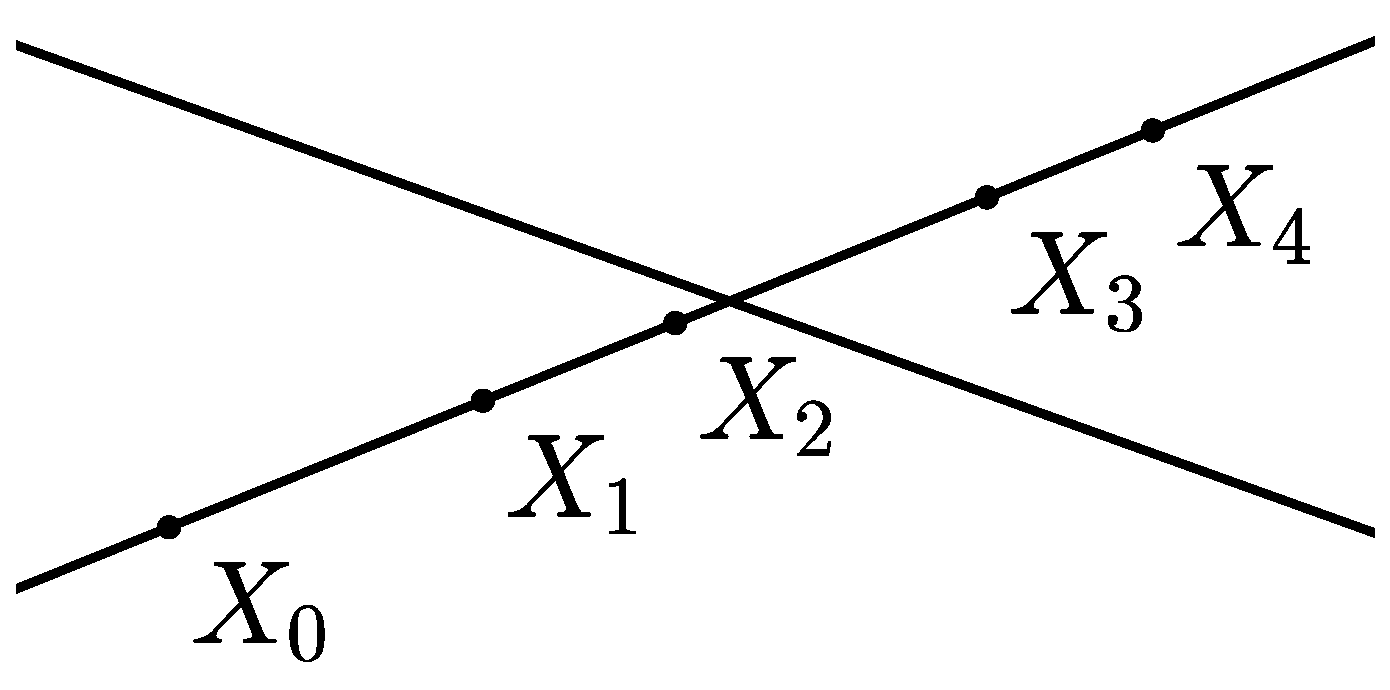
\includegraphics[scale=.15]{Graficos/alineados5.eps}
		\caption{Ilustración de una de las cónicas que pasan por cinco puntos alineados.}
		\label{C8_img_alineados5}
	\end{figure}
	
	Por ende, una restricción que debemos imponer a los $5$ puntos para que estos identifiquen a una única cónica es que no estén alineados.
\subsubsection{Cuatro Puntos Alineados}
	Continuando con esta idea de jugar con los casos extremos, tomo un conjunto de $5$ puntos de los cuales $4$ de ellos están alineados.
	
	Si tomamos la recta que pasa por los cuatro primeros puntos y una recta cualquiera que pase por el quinto, tenemos una cónica.
	
	\begin{figure}[h]
		\centering
		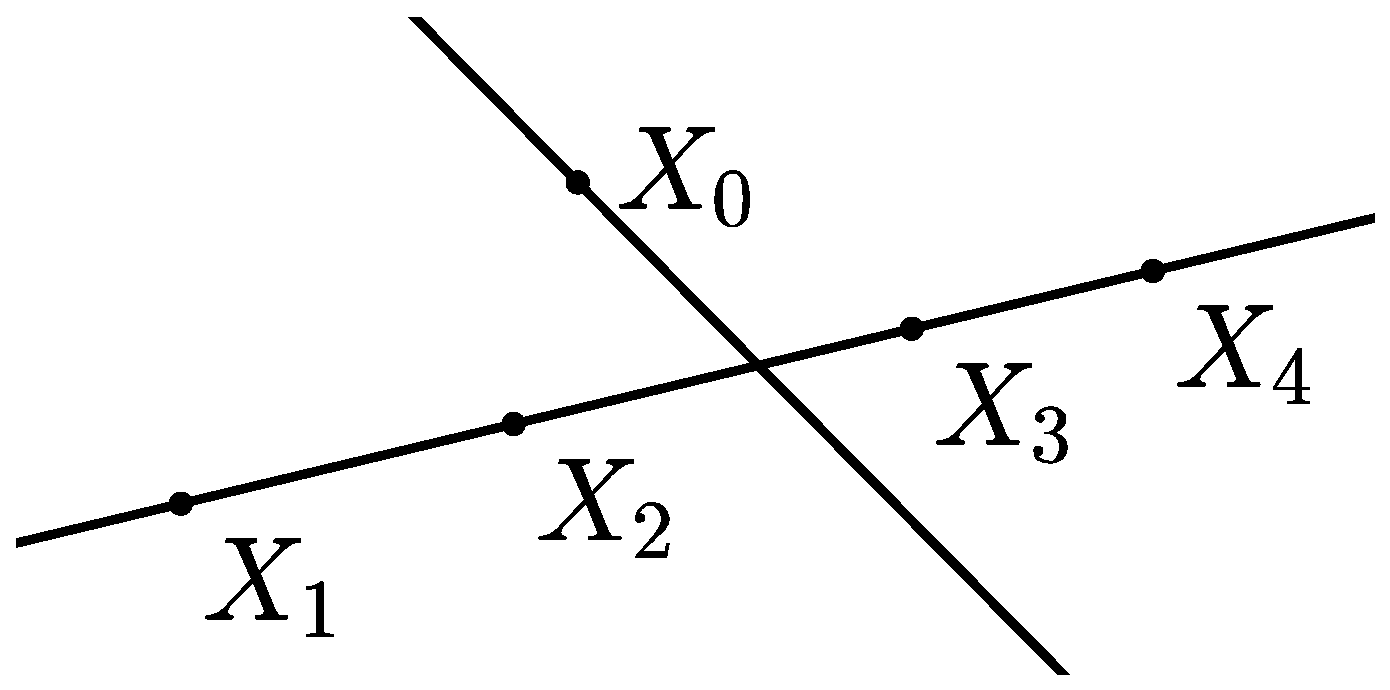
\includegraphics[scale=.15]{Graficos/alineados4.eps}
		\caption{Ilustración de una de las cónicas que pasan por cuatro puntos alineados.}
		\label{C8_img_alineados4}
	\end{figure}
	
	Esta cónica tampoco es única ya que la elección de la segunda recta es arbitraria de entre las sectas del haz con base el quinto punto. Por tanto, aquí tenemos una condición mas a excluir.
	
	Por tanto las condiciones que impongamos para que $5$ puntos determinen totalmente una cónica deben prohibir que esto suceda.
	
\subsubsection{Tres Puntos Alineados}
	Continuemos con nuestra particular danza al borde del abismo y tomemos un conjunto de $5$ puntos de los cuales $3$ de ellos estén alineados.
	
	Una posible cónica que pase por estos puntos es la formada por la recta en la se encuentran los $3$ puntos alineados y la recta que une los dos restantes.
	
	\begin{figure}[h]
		\centering
		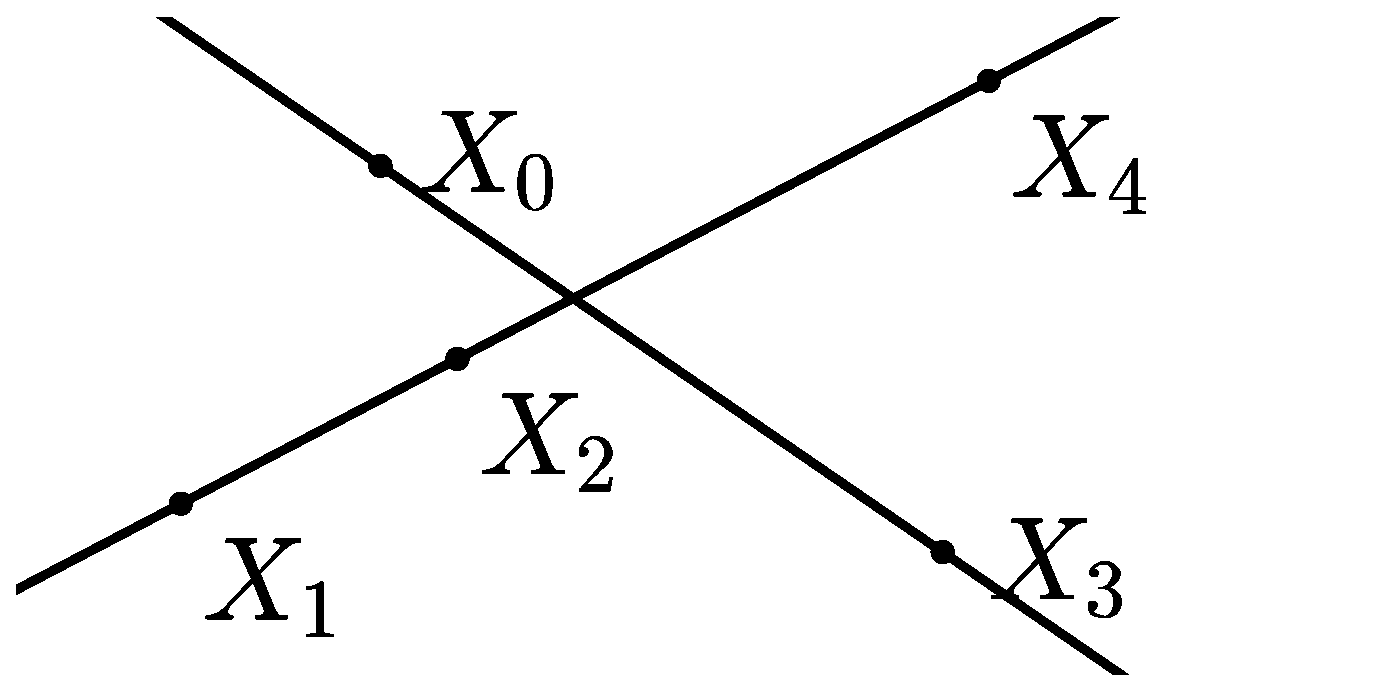
\includegraphics[scale=.15]{Graficos/alineados3.eps}
		\caption{Ilustración de la cónica que pasa por tres puntos alineados.}
		\label{C8_img_alineados3}
	\end{figure}
	
	Por primera vez, hemos obtenido una construcción única, sin embargo, uno podría preguntarse si no hay más cónicas (no degeneradas) que pasen por dichos puntos.
	
	La respuesta es no, y puede comprobarse siguiendo el procedimiento presentado en el apartado \ref{C8_intento} (se deja al lector la comprobación).
	
	Esto nos da, por así decirlo un golpe de moral para intentar demostrar el teorema, ya que podríamos imponer como condición a los puntos que $4$ de ellos no estén alineados. Así lo haremos.
\subsubsection{Teorema de Determinación}
Pasemos pues a enunciar y demostrar el teorema de determinación de una cónica por $5$ puntos, cuya demostración puede parecer larga, pero realmente es muy simple.
\begin{theo}[Teorema de Determinación]
	\label{C8_teo_determinacion}
	Dados $5$ puntos distintos de $\proy(E)$, no estando $4$ de ellos alineados, hay una única cónica que pasa por ellos.
\end{theo}
\begin{proof}
	Sean los puntos $X_0,X_1,X_2,X_3,X_4$.
	
	Como no hay $4$ puntos alineados, habrá $3$ que formen un triángulo, el cual tomaremos como parte de una referencia.
	
	Podemos suponer sin pérdida de generalidad que $X_0,X_1,X_2$ forman un triángulo. De esta forma tenemos
	\begin{equation}
		\mf{R}=\{X_0,X_1,X_2;e\}
	\end{equation}
	para cierto punto unidad $e$.
	
	Recordemos brevemente que las coordenadas de $X_0,X_1,X_2$ en la referencia $\mf{R}$ son
	\begin{equation*}
		\begin{array}{ccc}
			X_0=(1:0:0)_{\mf{R}}\qquad &\qquad X_1=(0:1:0)_{\mf{R}} \qquad&\qquad X_2=(0:0:1)_{\mf{R}}
		\end{array}
	\end{equation*}
	
	Si hubiera una cónica que pasara por los $5$ puntos, esta tendría cierta matriz simétrica $M$ que cumpla las restricciones
	\begin{equation}
		\begin{array}{ccc}
		\vec{X_0}^tM\vec{X_0}=0\qquad&\qquad
		\vec{X_1}^tM\vec{X_1}=0\qquad&\qquad
		\vec{X_2}^tM\vec{X_2}=0
		\end{array}
	\end{equation}
	Para cualesquiera representantes vectoriales de $X_0,X_1,X_2$.
	
	Si consideremos que la matriz $M$ viene dada por
	\begin{equation*}
		M=\begin{pmatrix}
			a & h & g\\
			h & b & f\\
			g & f & c
		\end{pmatrix}
	\end{equation*}
	y echamos las cuentas correspondientes a las restricciones obtenemos que
	\begin{equation*}
		a=0\qquad\qquad b=0\qquad\qquad c=0
	\end{equation*}

Así, usando la ecuación \ref{C8_eq_polinomio} obtenemos que la ecuación que nos define la cónica es de la forma
\begin{equation}
	fyz+gxz+hxy=0
\end{equation}

	Llegados a este punto se nos pueden presentar dos situaciones. La primera es que podamos coger como punto unidad alguno de los cinco puntos originales. El otro caso es el complementario.
	\begin{enumerate}
		\item Si alguno de los puntos restantes no se encuentra sobre los lados del triángulo, podemos tomar dicho punto como punto unidad de nuestra referencia $\mf{R}$. 
		
		Supongamos sin pérdida de generalidad que $X_3$ no se encuentra sobre los lados del triángulo.
		
		En tal caso, tomando a $X_3$ como punto unidad, es claro que sus coordenadas respecto de la referencia $\mf{R}$ serán
		\begin{equation*}
			X_3=(1:1:1)_{\mf{R}}
		\end{equation*}
		Como la cónica también debe pasar por $X_3$, la matriz $M$ deberá verificar la restricción
		\begin{equation*}
			\vec{X_3}^tM\vec{X_3}=0
		\end{equation*}
		Si echamos las cuentas, esto nos arroja que se debe cumplir que
		\begin{equation*}
			f+g+h=0
		\end{equation*}
		Como la cónica también ha de pasar por $X_4=(x_4,y_4,z_4)_{\mf{R}}$, la matriz de la cónica debe cumplir la restricción adicional
		\begin{equation*}
			y_4z_4f+x_4z_4g+x_4y_4h=0
		\end{equation*}
	En definitiva, tenemos un sistema homogéneo de ecuaciones lineales que tiene por matriz de coeficientes
	\begin{equation}
		\begin{pmatrix}
		1 & 1 & 1\\
		y_4z_4 & x_4z_4 & x_4y_4
		\end{pmatrix}
	\end{equation}
	Como ya adelantamos, para que la cónica sea única, el rango de esta matriz deberá ser $2$. Para comprobar este hecho, supongamos que el rango es $1$, es decir, que se anulan todos los menores de orden $2$ de la matriz.
	
	Haciendo esto, obtenemos el siguiente sistema de ecuaciones
	\begin{equation}
		\left\{
			\begin{array}{l}
			x_4z_4-x_4y_4=0\\
			x_4y_4-y_4z_4=0\\
			y_4z_4-x_4z_4=0
			\end{array}
		\right.\leadsto\left\{
		\begin{array}{l}
		x_4(z_4-y_4)=0\\
		y_4(x_4-z_4)=0\\
		z_4(y_4-x_4)=0
		\end{array}
		\right.
	\end{equation}
	Comencemos analizando la primera ecuación.
	
	Si $x_4=0$ entonces, por la segunda ecuación, $y_4z_4=0$, como $y_4$ y $z_4$ son elementos de un cuerpo, alguno de los dos será nulo. Esto implica que $X_4$ tiene las mismas coordenadas homogéneas (salvo múltiplos) que $X_1$ o $X_2$, lo cual es absurdo por ser todos los puntos distintos.
	
	Si por el contrario $z_4=y_4$, por la segunda ecuación se tiene que $x_4=z_4$, en tal caso $X_4$ tendría las mismas coordenadas homogéneas que $X_3$, lo cual vuelve a ser absurdo.
	
	Por ende, en este caso, el rango de la matriz es $2$ y la cónica que pasa por los $5$ puntos es única.
		\item Si $X_3$ y $X_4$ están sobre los lados del triángulo de referencia, es claro que no pueden pertenecer al mismo lado, ya que si no habría $4$ puntos alineados.
		
		Podemos suponer que $X_3$ está sobre la recta $l:X_0X_1$ y que $X_4$ está sobre la recta $m:X_1X_2$.
		
		Es claro que el producto de rectas $lm$ es una cónica que contiene a los cinco puntos. Veamos que es única.
		
		Observamos que las coordenadas de $X_3$ y $X_4$ respecto de $\mf{R}$ son
		\begin{equation}
			X_3=(x_3:y_3:0)_{\mf{R}}\qquad \qquad X_4=(0:y_4:z_4)_{\mf{R}}
		\end{equation}
		Si forzamos a la cónica a pasar por $X_4$, aplicando la restricción pertinente y echando las cuentas tendríamos que
		\begin{equation*}
			fy_4z_4=0
		\end{equation*}
		Esto fuerza a que $f=0$ ya que si se anularan $y_4$ o $z_4$ el punto $X_4$ pasaría a tener las mismas coordenadas homogéneas que $X_1$ o $X_2$, lo cual es imposible.
		
		Si adicionalmente forzamos a la cónica a pasar por $X_3$ obtendríamos que debe cumplirse que
		\begin{equation*}
			hx_3y_3=0
		\end{equation*}
	Por un argumento simétrico al anterior obtenemos que $h=0$.
	Así pues la cónica es única, ya que es la que tiene por rayo de matrices asociadas
	\begin{equation}
		\begin{pmatrix}
		0 & 0 & g\\
		0 & 0 & 0\\
		g & 0 & 0
		\end{pmatrix}
	\end{equation}
	Que es precisamente la matriz del producto de rectas $lm$.
	\end{enumerate}
Con lo que concluye la prueba.
\end{proof}
En el siguiente apartado daremos una vuelta de tuerca adicional al resultado anterior, que pondrá de manifiesto la relevancia de poder pensar en las cónicas como puntos de un espacio proyectivo de dimensión $5$.
\subsection{Haces de Cónicas}
El objetivo de este apartado es estudiar el conjunto de cónicas que pasan por cuatro puntos no alineados. El estudio de estas cónicas nos llevará a un método de cálculo más sencillo para determinar la cónica que pasa por $5$ puntos.

En primer lugar, trabajemos sobre algunos conceptos auxiliares.
\begin{obs}[Recta de Cónicas]
Sean $\mc{C}_1$ y $\mc{C}_2$ dos cónicas distintas vistas como dos puntos de $\proy^5$.

Consideramos la recta de $\proy^5$ que pasa por $\mc{C}_1$ y $\mc{C}_2$. Esta recta queda parametrizada por
\begin{equation}
	\mc{C}_1\mc{C}_2:\class{\vec{\mc{C}_1}+\theta\vec{\mc{C}_2}}
\end{equation}
donde $\theta\in\overline{\K}$ y $\vec{\mc{C}_1}$, $\vec{\mc{C}_2}$ son representantes vectoriales de dichas cónicas en el espacio vectorial de las matrices simétricas $\mathrm{Sim}(3)$.

Es decir, acabamos de definir una ``\ti{recta de cónicas}'' a partir de dos cónicas.
\end{obs}
Nuestro objetivo ahora es demostrar que dados $4$ puntos no alineados cualesquiera, estos determinan totalmente una recta de cónicas.

Para demostrar esto iremos por partes. En primer lugar veremos que por $4$ puntos no alineados siempre podremos trazar dos cónicas distintas $\mc{C}_1$ y $\mc{C}_2$.

Tras esto, nos preguntaremos si, en caso de poder trazar otras dos cónicas distintas por dichos cuatro puntos $\mc{C}_1'$ y $\mc{C}_2'$, la recta $\mc{C}_1'\mc{C}_2'$ es la misma que la recta $\mc{C}_1\mc{C}_2$.

Adicionalmente, veremos que todas cónicas de la recta $\mc{C}_1\mc{C}_2$ pasan por los cuatro puntos iniciales.
\subsubsection{Construcción de Dos Cónicas por Cuatro Puntos}
Sean $A,B,C,D$ cuatro puntos no alineados. Es claro que estos puntos no determinan una única cónica ya que siempre puedo trazar dos cónicas distintas, y especialmente simples, que pasen por los cuatro puntos. En efecto, estas cónicas son
\begin{equation}
	\label{C8_eq_construccion}
	\mc{C}_1=AB\cdot CD\qquad\qquad\mc{C}_2=AC\cdot BD
\end{equation}
\begin{figure}[h]
	\centering
	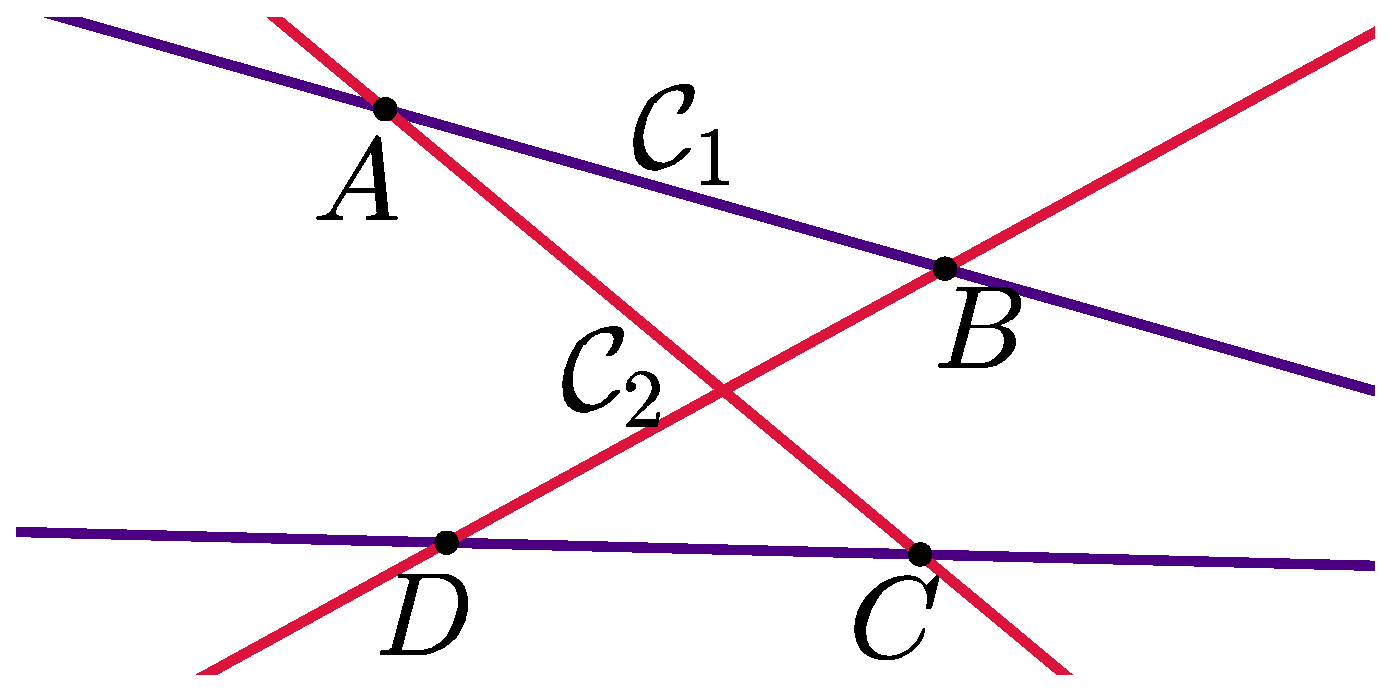
\includegraphics[scale=.2]{Graficos/haz1.eps}
	\caption{Ilustración de dos cónicas que pasan por $4$ puntos.}
	\label{C8_img_haz1}
\end{figure}
La comprobación de que ambas cónicas pasan por los cuatro puntos es trivial, ya que $\mc{C}_1=AB\cup CD$. Es decir, contiene a la recta $AB$, luego también contiene a $A$ y a $B$. Asimismo contiene a la recta $CD$, luego por supuesto a los puntos $C$ y $D$. Análogamente se comprueba para la otra cónica.

Queda ahora asegurarse de que estas cónicas son siempre distintas. Esta comprobación se basa en que ambas cónicas pueden ser vistas como conjuntos de dos rectas. Por ende, la cónica $\mc{C}_1$ será igual a la cónica $\mc{C}_2$ si y solo si la recta $AB$ es igual a la recta $AC$ o bien a la recta $BD$. Suponiendo que $AB=AC$ obtenemos que los puntos $A$, $B$ y $C$ están alineados y que la recta $CD$ es igual a la recta $BD$, de donde se desprende que $C$, $B$ y $D$ están alineados. De aquí concluimos que los $4$ puntos están alineados y por tanto llegamos a una contradicción. La comprobación del otro caso es totalmente simétrica.
\subsubsection{Cuatro Puntos Determinan una Recta de Cónicas}
Para probar que dados dos pares de cónicas $(\mc{C}_1,\mc{C}_2)$ y $(\mc{C}_1',\mc{C}_2')$ que pasan por los puntos $A,B,C,D$ las rectas $\mc{C}_1\mc{C}_2$ y $\mc{C}_1'\mc{C}_2'$ son iguales basta con reeditar la demostración del teorema de determinación (teorema \ref{C8_teo_determinacion}). Lo haremos sin dar demasiados detalles.

Tomamos como triángulo de referencia tres puntos no alineados de los cuatro iniciales. Renombrando los puntos si es preciso, podemos suponer que $A$, $B$ y $C$ forman un triangulo de referencia. Hecho esto, distingamos dos casos.

Si puedo tomar $D$ como punto unidad, al exigirle a una matriz genérica de cónica que pase por los $4$ puntos obtengo que esta debe cumplir las siguientes restricciones.
\begin{equation*}
	\left\{\begin{array}{c}
	a=0\\
	b=0\\
	c=0\\
	f+g+h=0
	\end{array}\right.
\end{equation*}
El conjunto de matrices que satisfacen dichas restricciones es un plano de $\mathrm{Sim}(3)$, luego una única recta de cónicas en $\proy^5$.

Si no puedo tomar $D$ como punto unidad se obtienen las ecuaciones
\begin{equation*}
	\left\{\begin{array}{c}
		a=0\\
		b=0\\
		c=0\\
		f=0
	\end{array}\right.
\end{equation*}
que son, de nuevo, las ecuaciones cartesianas de un plano de $\mathrm{Sim}(3)$.
En conclusión, toda cónica que pasa por cuatro puntos pertenece a la misma recta de cónicas.

Nótese que esta demostración también nos hubiera valido para demostrar que siempre podemos trazar dos cónicas distintas por $4$ puntos no alineados, sin embargo, la prueba que dimos antes nos proporciona una construcción explícita más útil.
\begin{obs}[Haces de Cónicas]
	Adicionalmente observamos que dadas dos cónicas que pasan por $4$ puntos y la recta de cónicas definida por ellas, todas las cónicas de la recta pasan por los cuatro puntos.
	
	Esto se debe a que las cónicas que pasan por $4$ puntos son una recta de cónicas (como acabamos de demostrar), luego la variedad generada por dos cónicas de la recta estará contenida en la recta de las cónicas que pasan por los cuatro puntos (y de hecho, obviamente es esa recta).
\end{obs}

Para concluir simplemente cabe mencionar que, como $4$ puntos identifican unívocamente una recta de cónicas tal que todas las cónicas de la recta pasan por dichos $4$ puntos, se suele decir que la recta de cónicas que pasa por dichos cuatro puntos es un ``\ti{haz de cónicas}'' con base esos cuatro puntos. Si dichos cuatro puntos son $A$, $B$, $C$ y $D$ normalmente escribiremos
\begin{equation}
	\haz(A,B,C,D)
\end{equation}

\begin{figure}[h]
	\centering
	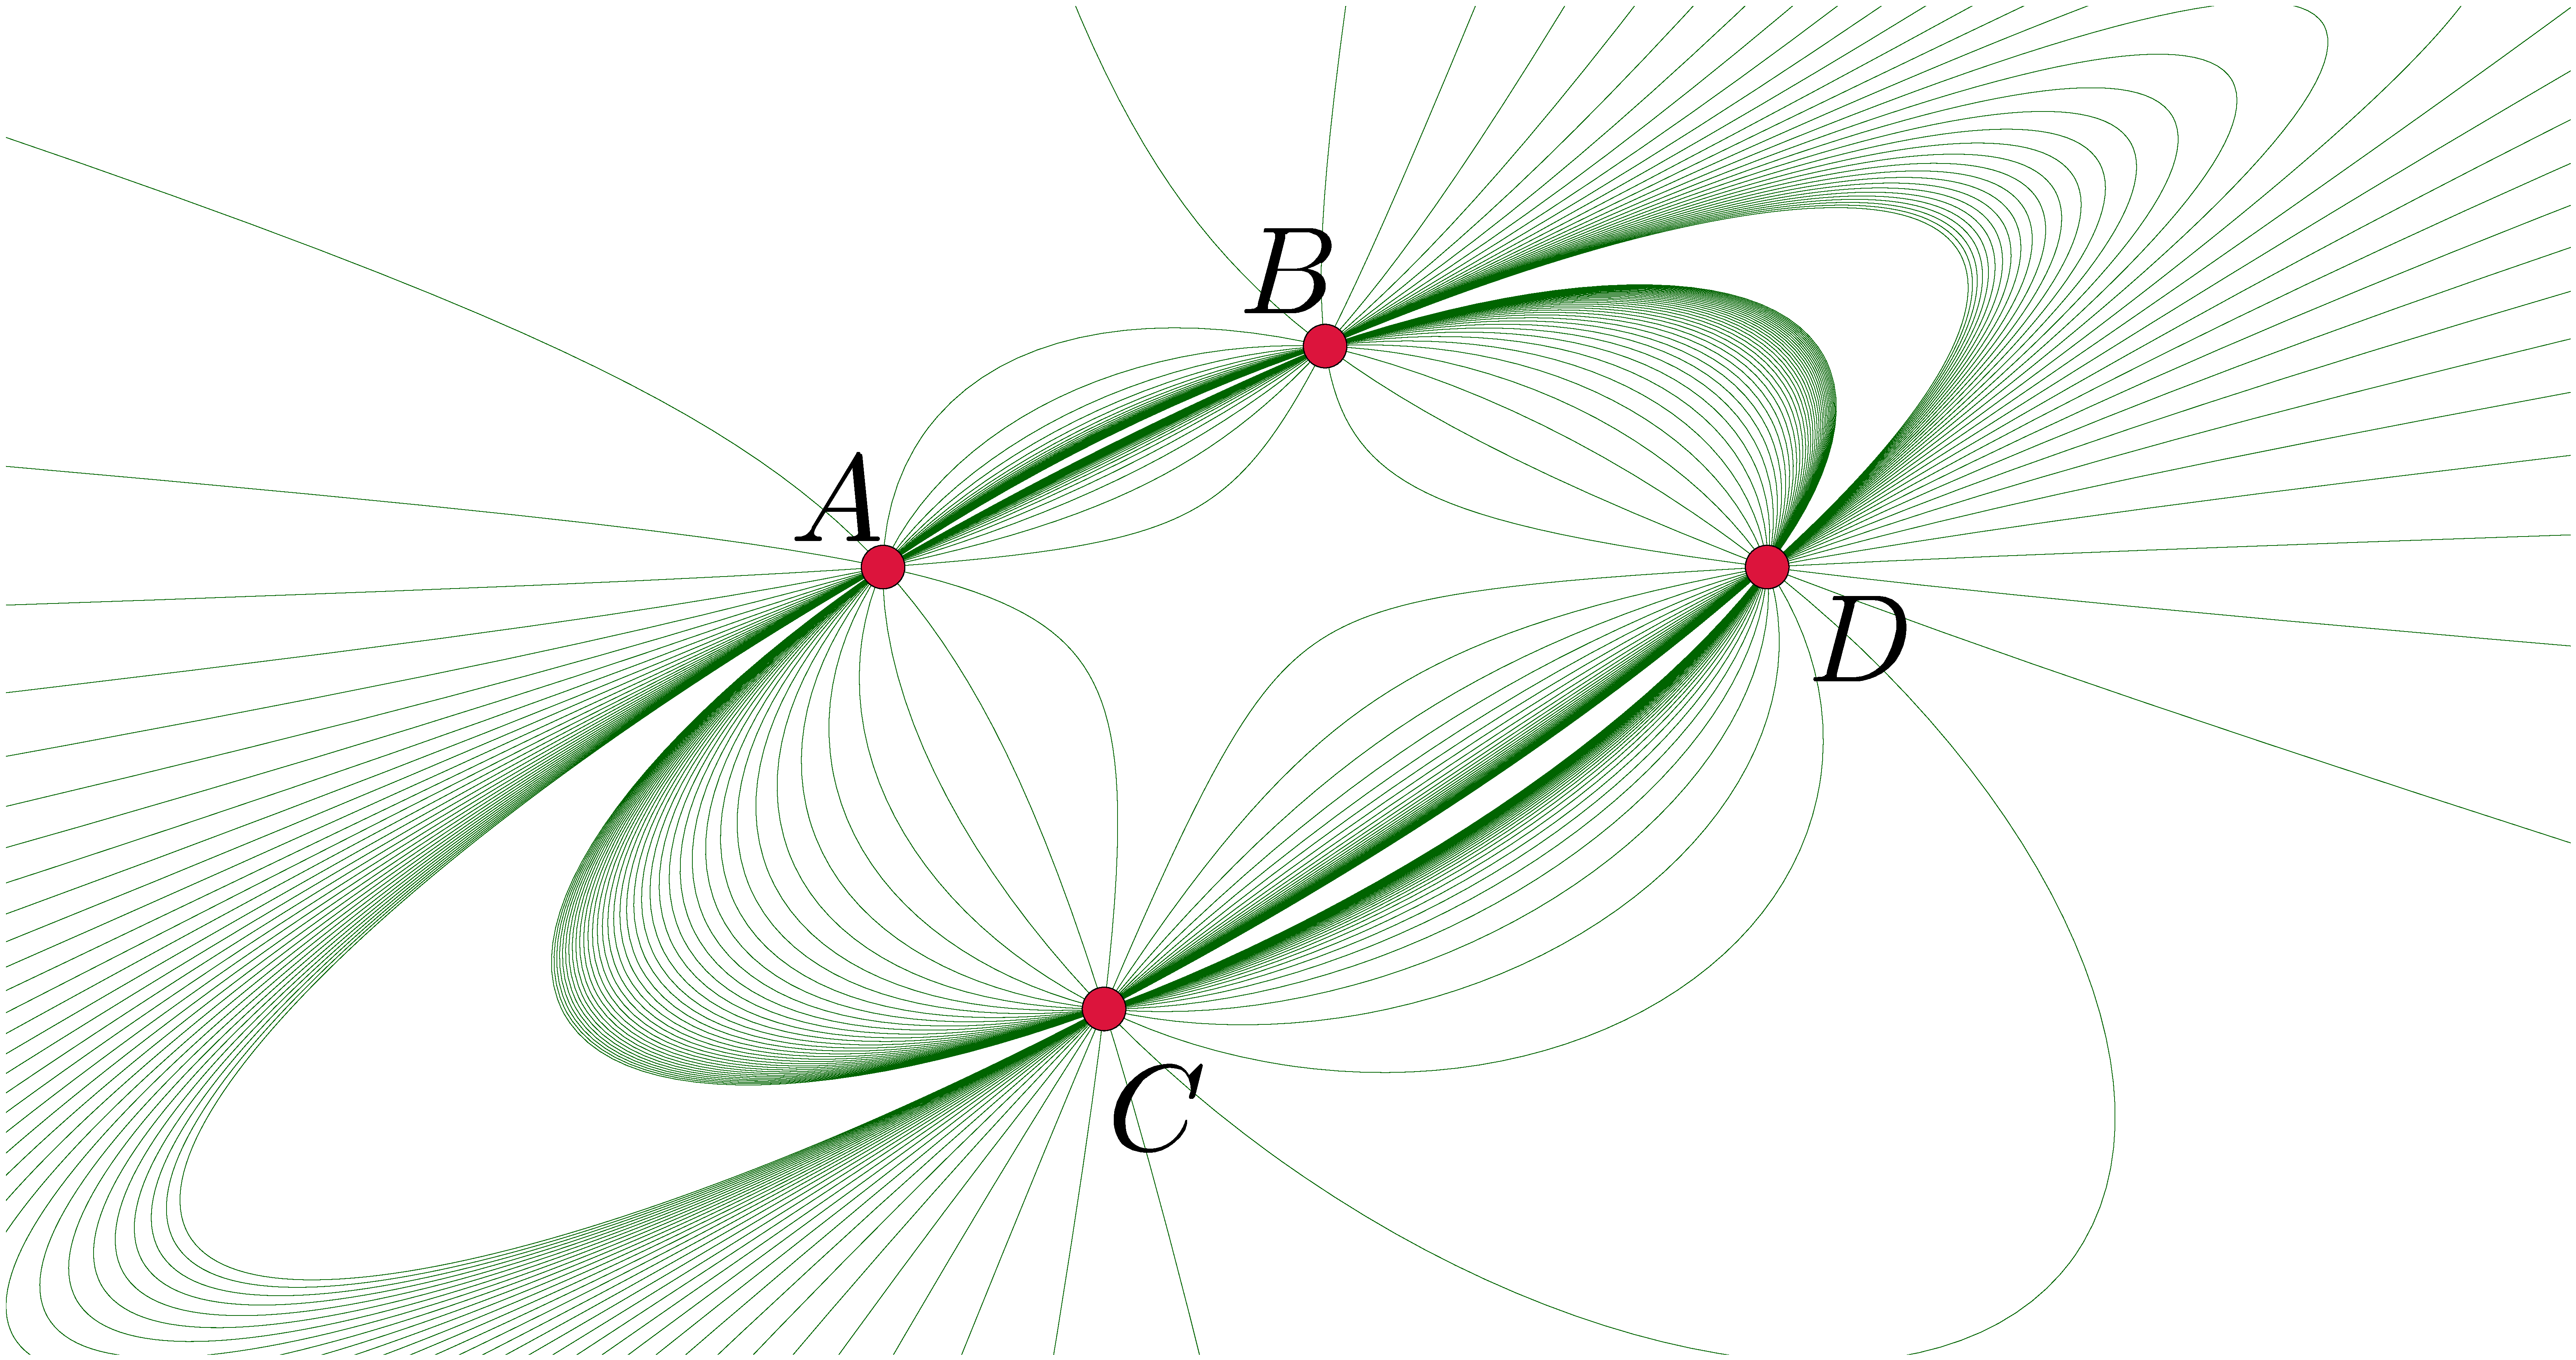
\includegraphics[scale=.05]{Graficos/HazDeConicasPorCuatroPuntos.eps}
	\caption{Ilustración algunas de las cónicas de $\haz(A,B,C,D)$}
	\label{C8_img_haz2}
\end{figure}

La utilidad de los haces de cónicas es similar a la utilidad de los haces de rectas, y es que permiten calcular de la cónica que pasa por $5$ puntos de una forma bastante sencilla. Veámoslo con un ejemplo.
\begin{exa}[Cálculo de la Cónica que Pasa por Cinco Puntos]
	Sean los puntos escritos en coordenadas no homogéneas respecto de alguna referencia $\mf{R}$.
	\[\begin{array}{ccc}
		A=(1,1)&&B=(1,0)\\
		C=(-1,2)&&D=(0,0)\\
		&E=(-3,2)&
	\end{array}\]
	Construyamos el haz de cónicas que pasa por los puntos $A,B,C,D$ usando la construcción de la ecuación \eqref{C8_eq_construccion}.
	
	Echando las cuentas obtenemos las ecuaciones que definen a las cónicas $AB\cdot CD$ y $AC\cdot BD$. Estas son
	\begin{equation*}
		\begin{array}{cc}
			AB\cdot CD : \qquad&\qquad AC\cdot BD :
		\end{array}
	\end{equation*}
\end{exa}

Llamamos la atención de que aún no hemos probado que toda recta de cónicas pueda ser identificada por $4$ puntos. Es algo que dejamos pendiente para el futuro. 
\section{Clasificación de las Cónicas No Degeneradas}
En esta sección se realizará una clasificación de las cónicas proyectivas en función de su número de puntos de corte con la recta del infinito, a la que denotaremos $l_\infty$.

Como ya adelantamos, en el espacio proyectivo no hay noción canónica de \ti{hiperplano del infinito} (en el sentido que podríamos coger el que quisiéramos), sin embargo, un convenio bastante ampliamente aceptado es tomar el hiperplano de ecuación cartesiana $z=0$ como hiperplano del infinito, en nuestro caso, como recta del infinito.

En definitiva, consideremos la siguiente clasificación, que justificaremos a lo largo del capítulo:
\begin{itemize}
	\item \tb{Tipo \ti{Elíptico}}: La cónica no tiene puntos de corte con $\l_{\infty}$. Normalmente denominaremos \ti{elipses} a estas cónicas.
	\item \tb{Tipo \ti{Hiperbólico}}: La cónica corta en dos puntos reales a $l_\infty$. A estas cónicas se las suele denominar \ti{hipérbolas}.
	\item \tb{Tipo \ti{Parabólico}}: La cónica corta en un único punto a la $l_\infty$. Se suele decir en este caso que la cónica es \ti{tangente} a la recta del infinito. Las cónicas de este tipo reciben el nombre de \ti{parábolas}.
\end{itemize}
\begin{figure}[h]
	\centering
	\subfigure[Elipse]{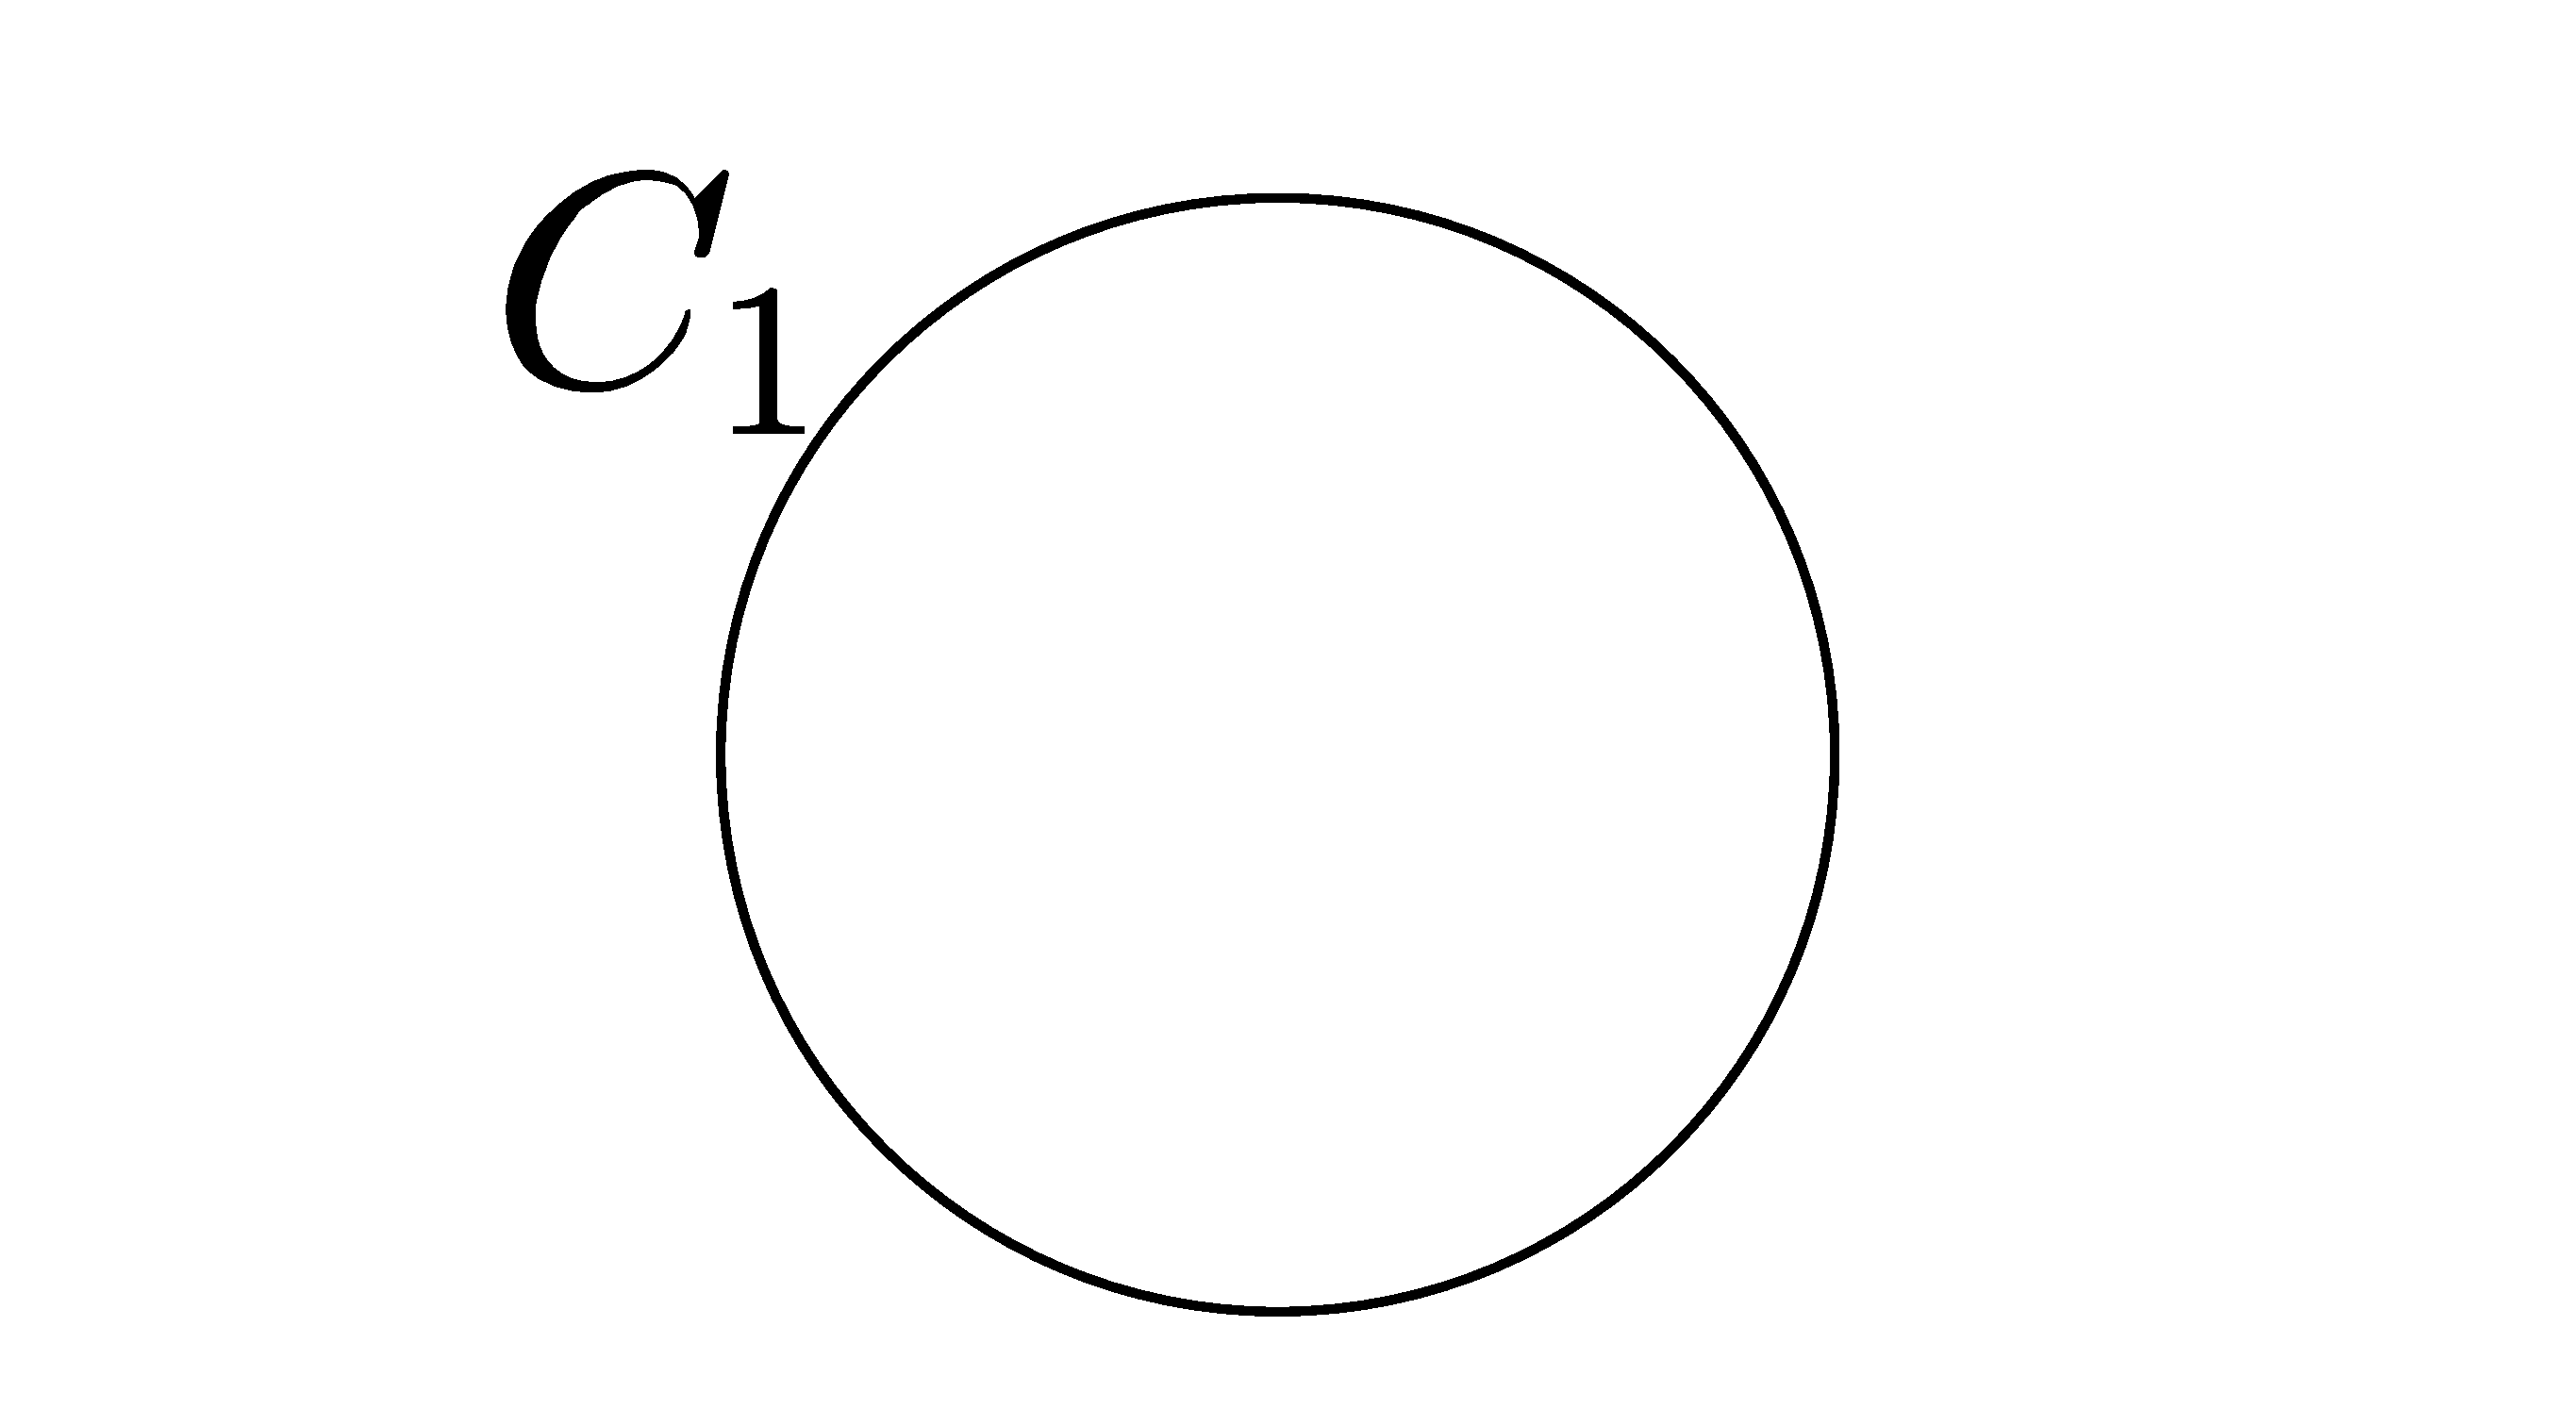
\includegraphics[scale=.065]{Graficos/elipse.eps}}
	\subfigure[Hipérbola]{
\includegraphics[scale=.028]{Graficos/hiperbola.eps}}
	\subfigure[Parábola]{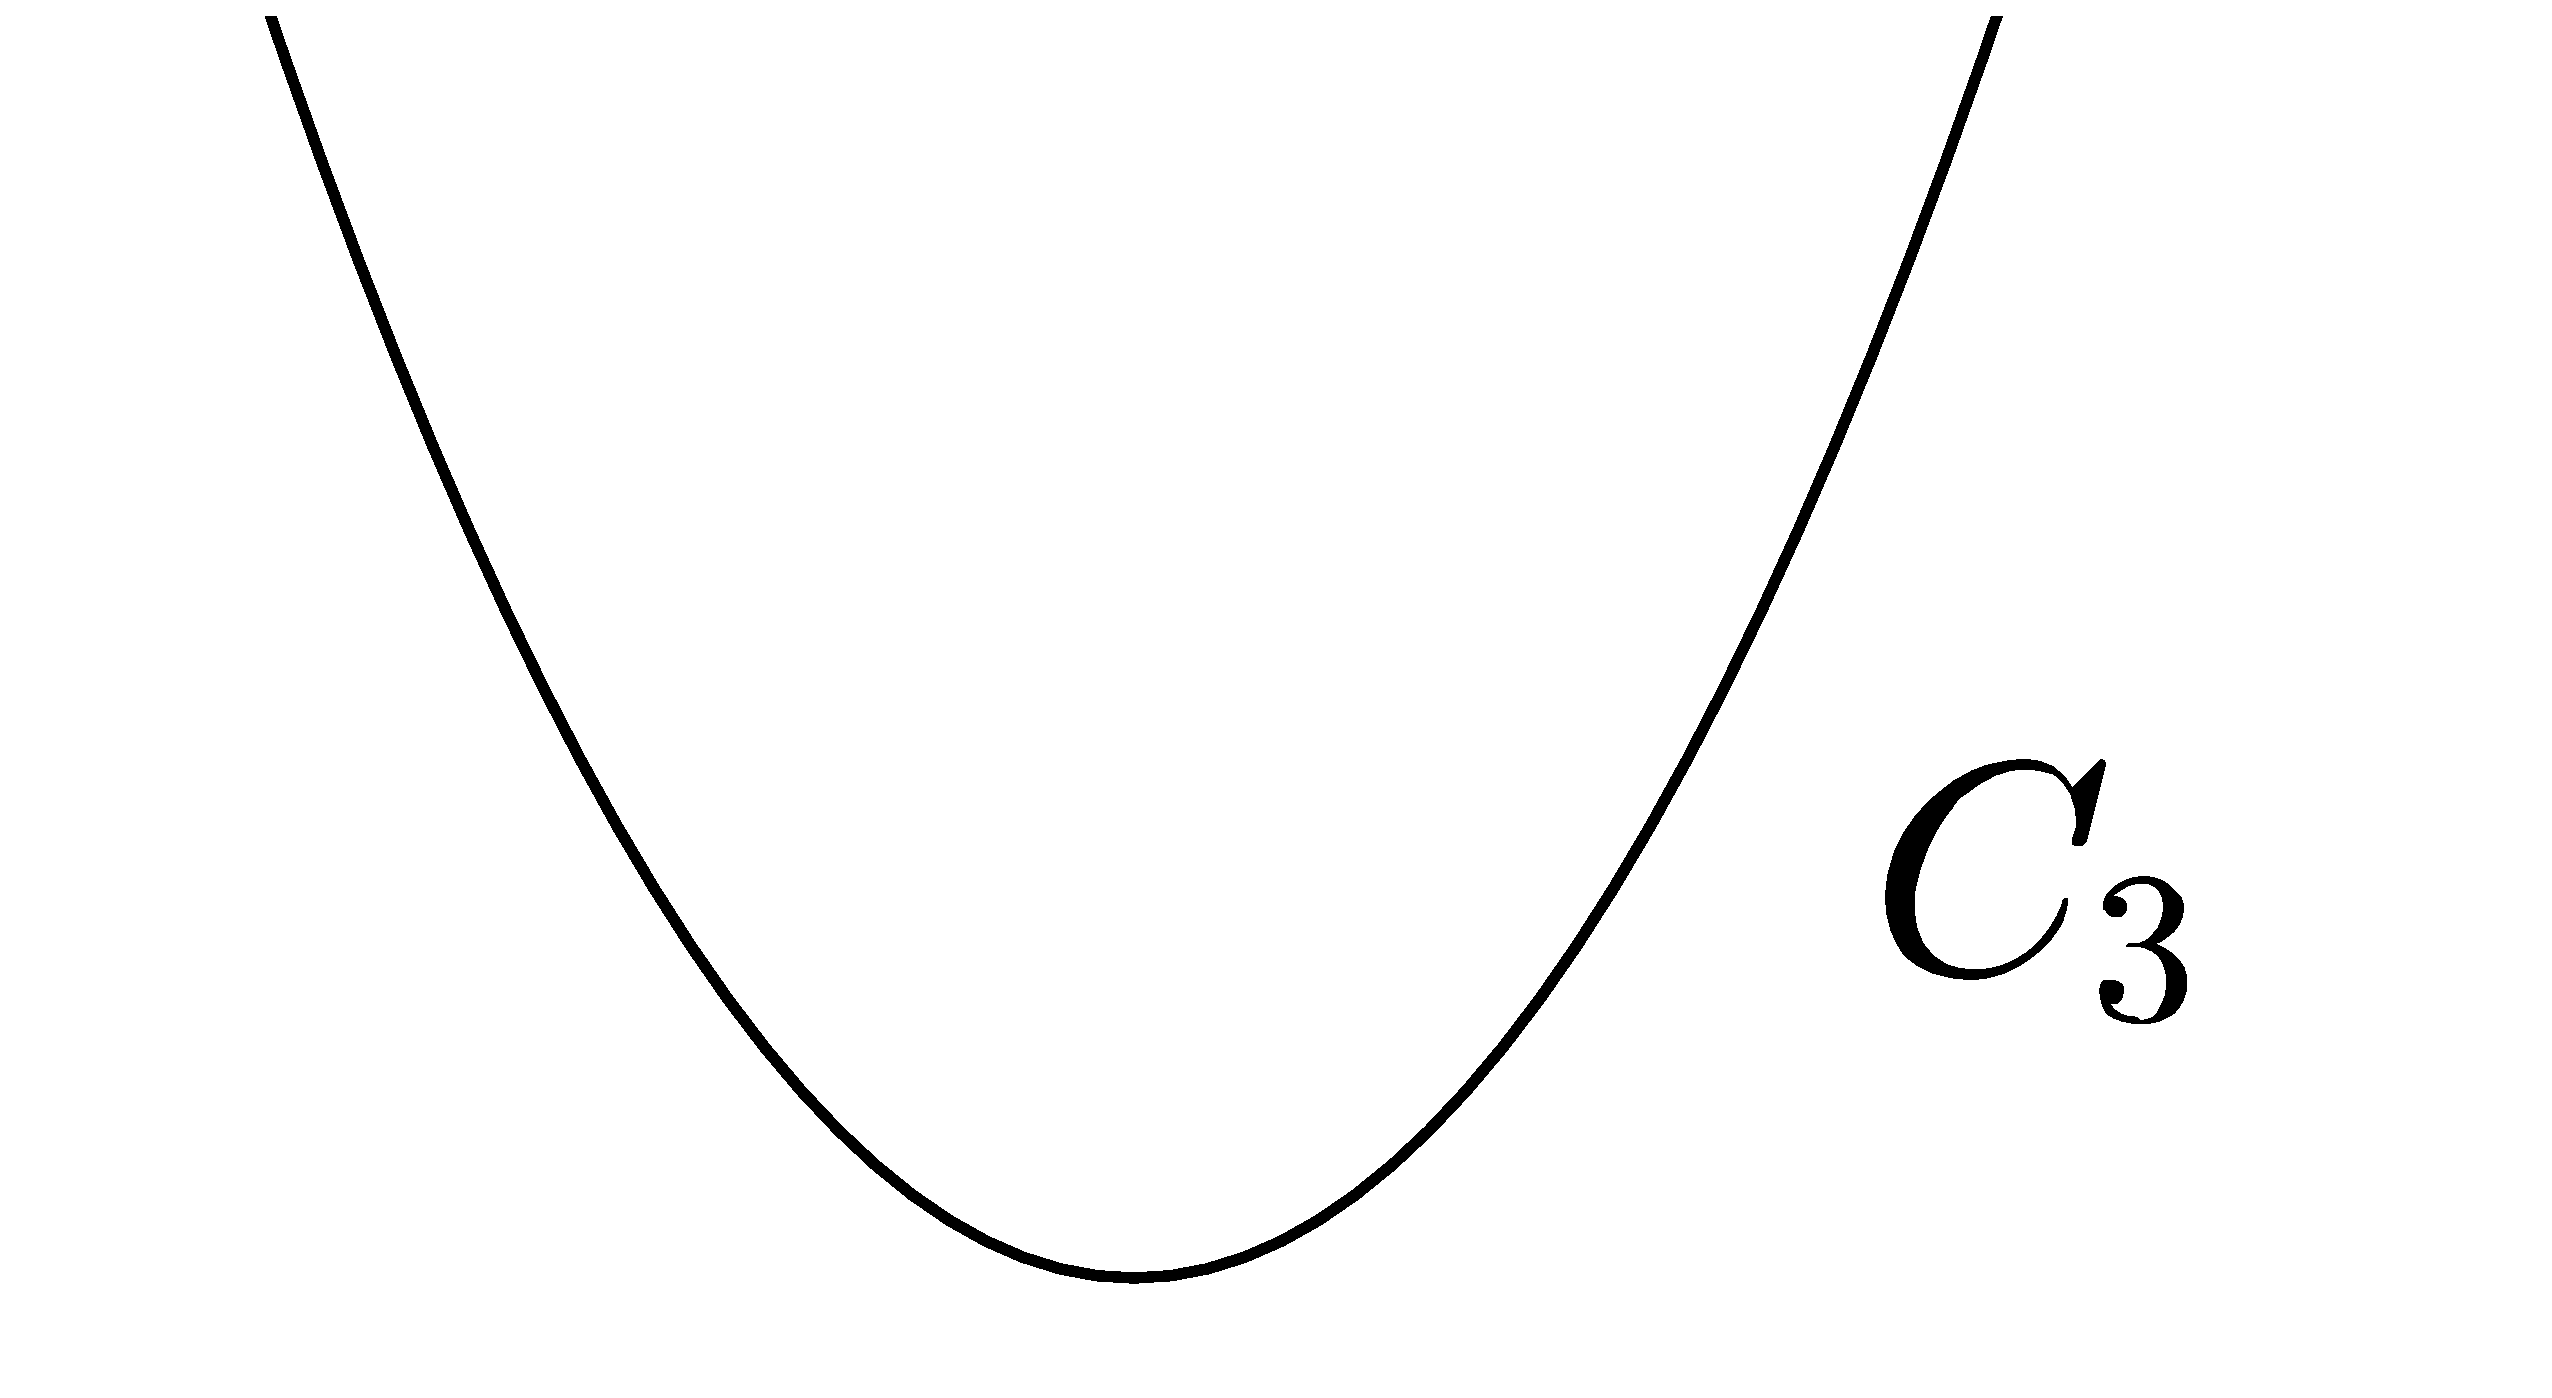
\includegraphics[scale=.06]{Graficos/parabola.eps}}
	\caption{Ilustración de los tipos de cónicas.}
	\label{C7_img_tiposConicas}
\end{figure}
Para que esta clasificación no resulte demasiado abstracta al lector, pongamos un ejemplos de cónicas de cada uno de los tipos.
\begin{exa}[Elipse]
	\label{C8_exa_elipse}
	Consideramos la cónica dada por la siguiente ecuación:
	\[\mc{C}:x^2+y^2-z^2=0\]
	Intersequemos la cónica con la recta $l_\infty:z=0$ para poder clasificarla.
	\[\left.\begin{array}{c}
	x^2+y^2-z^2=0\\
	z=0
	\end{array}\right\}\leadsto x^2+y^2=0\]
	Es claro que la única solución a esta ecuación es el punto $(0,0,0)$, sin embargo, el rayo engendrado por este vector no está definido. Por ende, no hay ningún rayo (punto proyectivo) de la cónica que sea, a la vez, un rayo de la recta del infinito. Por ende, esta cónica es una elipse.
\end{exa}
\begin{exa}[Hipérbola]
	Clasifiquemos la cónica de ecuación:
	\[\mc{C}:X^2-Y^2=1\]
	Antes de que cunda el pánico, nótese que esta ecuación nos viene dada en forma ``deshomogeneizada'' (si no no sería la ecuación de una cónica). Al homogeneizarla nos queda algo bastante más familiar:
	\[\mc{C}:x^2-y^2-z^2=0\]
	Calculemos los puntos de corte con $z=0$:
	\[\left.\begin{array}{c}
	x^2-y^2-z^2=0\\
	z=0
	\end{array}\right\}\leadsto x^2=y^2\]
	Tomando raíces cuadradas y considerando todos los casos necesarios obtemos como soluciones los puntos de la forma:
	\[\begin{array}{cc}
	\class{(\lambda,\lambda,0)}=(1:1:0)\qquad & \qquad \class{(\lambda,-\lambda,0)}=(1:-1:0)
	\end{array}\]
	Por ende, la cónica $\mc{C}$ tiene dos puntos de corte con la recta del infinito, esto significa que es de tipo hiperbólico.
\end{exa}
\begin{exa}[Parábola]
	Se nos da la siguiente cónica en forma no homogénea:
	\[\mc{C}:Y=X^2\]
	Calculemos (tras homogeneizar) los puntos de corte de la misma con $l_\infty$.
	\[\left.\begin{array}{c}
	zy-x^2=0\\
	z=0
	\end{array}\right\}\leadsto x^2=0\]
	Teniendo en cuenta esto, los puntos que cumplen las restricciones impuestas por ambas ecuaciones son los de la forma $(0,\lambda,0)$ (los cuales, además, son solución doble). Estos generan un único rayo. Por ende, la cónica y la recta del infinito únicamente se cortan en un punto. Esto es lo mismo que decir que $\mc{C}$ es una parábola.
\end{exa}

\section{Cuádricas, cónicas y cambio de referencia}
Hasta ahora hemos hablado de cuádricas y su matriz asociada en cierta referencia proyectiva. Pero ¿y si queremos escribir la ecuación de la cuádrica o su matriz en otra referencia? A continuación veremos como hacer esto.\\

Sean dos referencias proyectivas $\mf{R}$ y $\overline{\mf{R}}$ del espacio proyectivo $\proy^n$. El cambio de la referencia $\mf{R}$ a $\overline{\mf{R}}$ viene descrito por las siguientes ecuaciones
\begin{equation}
\rho X=M\overline{X}
\end{equation}
donde $M$ es la matriz de paso. 

Partimos de una cuádrica que en la referencia $\mf{R}$ tiene ecuaciones
\begin{equation}
X^tAX=0
\end{equation}
donde $A$ es la matriz de la cuádrica en esta referencia. Nuestro objetivo es escribir la cuádrica en la referencia $\overline{\mf{R}}$., es decir, buscamos la matriz $\overline{A}$ tal que
\begin{equation}
\overline{X}^t\overline{A}\overline{X}=0
\end{equation}
Para ello utilizamos las ecuaciones de cambio de referencia. Dado que la matriz de la cuádrica, y con ello su ecuación, es única salvo múltiplo, omitiremos el parámetro $\rho$ en los siguientes cálculos.
\begin{equation}
X^tAX=0\Leftrightarrow (M\overline{X})^tA(M\overline{X})=0\Leftrightarrow \overline{X}^t M^tAM\overline{X}=0
\end{equation}
Se concluye pues que la matriz de la cuádrica en la referencia $\overline{\mf{R}}$ es $M^tAM$. Por tanto, las ecuaciones que relacionan la matriz de la cuádrica en la referencia ${\mf{R}}$ con su matriz en la referencia $\overline{\mf{R}}$ son
\begin{equation}
\label{C8_eq_relacionMatrices_referencias}
\rho\overline{A}=M^tAM
\end{equation}
donde $M$ recordemos que es la matriz de cambio de referencia. Se observa que, si $A$ es simétrica, entonces $\overline{A}$ seguirá siendo simétrica. En efecto
\begin{equation}
(\rho\overline{A})^t=(M^tAM)^t=M^tA^tM=M^tAM=\rho\overline{A}
\end{equation}
Gracias a esto hallar los coeficientes de la matriz $\overline{A}$ pasa a ser una tarea sencilla. Particularicemos por un momento al caso en el que nos encontramos en $\proy^2$ para ver el gran cambio que esto supone.

Si $\overline{A}$ no fuese una matriz simétrica, al ser una matriz $3\times 3$, tendríamos $9$ parámetro a determinar, que se transformarían en $8$ si consideramos la proyección del espacio vectorial de las matrices $3\times 3$, es decir, si nos da igual considerar $\overline{A}$ o $\lambda\overline{A}$. En cambio, al ser simétrica estos se reducen a $5$, ya que, como vimos en la observación~\ref{C8_obs_conica_p5} , $\proy(\mathrm{Sim}(3))$ es isomorfo a $\proy^5$. Esto supone una gran diferencia frente a los $9$ parámetros iniciales. 

Recordemos, del ejemplo~\ref{C8_exa_coordenadas_conica_p5}, que, a su vez, estos coeficientes de la matriz $\overline{A}$ son las coordenadas de la cónica en $\proy^5$, con lo cual la cónica queda perfectamente determinada.\\

Este tipo de trasformaciones preservan el rango de la matriz. Esto se debe a que $A$ y $\overline{A}$ son congruentes, es decir, que existe una matriz $P$ tal que $\overline{A}=P^tAP$. Por tanto, en particular, son equivalentes.

Esto implica que, si partimos de una cónica no degenerada con matriz $A$ es imposible que al hacer un cambio en el sistema de referencia proyectivo obtengamos una matriz degenerada, pues $rg(A)=rg(\overline{A})$. Sin embargo, cabe esperar que mediante un cambio de referencia se pueda trasformar una cónica en cualquier otra (preservando la degeneración), como veremos más adelante.

\section{Cónicas degeneradas}
\label{C8_sec_conicas_degeneradas}
Al igual que hicimos con cónicas no degeneradas, realizaremos una clasificación de cónicas degeneradas. Aunque esta clasificación terminará siendo mucho más simple que la que tenemos para cónicas no degeneradas, llegar a ella conlleva más trabajo. Por ello, iremos desarrollando una serie de lemas y proposiciones que nos guiarán al resultado final. Comenzamos definiendo una cónica degenerada.
\begin{defi}
	Diremos que una cónica, dada por la ecuación
	\begin{equation}
	\mc{C}:X^tAX=0
	\end{equation}
	es \ti{degenerada} si contiene una recta.
\end{defi}

Esta definición de cónica degenerada no es muy manejable. Por ello, veamos la siguiente proposición
\begin{prop}\label{C8_prop_rango_menor_3_degenerada}
	Sea $\mc{C}$ una cónica cuya matriz en cierta referencia es $A$. Si $rg(A)<3$ entonces $\mc{C}$ es una cónica degenerada.
\end{prop}

\begin{proof}
	Para demostrar que la cónica $\mc{C}$ es degenerada veamos que contiene una recta. Si el rango de la matriz $A$ es menor que $3$, entonces el núcleo de $A$ no es vacío. Por tanto, existe un vector $y_0$ tal que $AY_0=0$, donde $Y_0$ representa el vector columna de $y_0$. Esto implica que $Y_0^tAY_0=0$, por lo que, al menos, el punto $[y_0]$ pertenece a la cónica.
	
	Sea $[z_0]$ otro punto de la cónica, distinto de $[y_0]$. Veamos que la recta $YZ$ generada por $[z_0]$ e $[y_0]$ está contenida en la cónica. Con esto quedaría demostrado que la cónica es degenerada.
	
	Sea un punto $[y_0+\theta z_0]$ de la recta $YZ$. Si este punto perteneciese a $\mc{C}$ para todo $\theta$, la recta $YZ$ estaría contenida en la cónica. Veamos que cumple la ecuación de la cónica, sea cual sea el valor de $\theta$:
	\begin{equation}\label{C8_eq_joanch_conicas_deg}
	(Y_0+\theta Z_0)^tA(Y_0+\theta Z_0)=Y_0^tAY_0+\theta Y_0^tAZ_0+\theta Z_0^tAY_0+\theta^2Z_0^tAZ_0=Y_0^tAY_0+2\theta Z_0^tAY_0+\theta^2Z_0^tAZ_0
	\end{equation}
	El primer y segundo sumando se anulan debido a que $y_0$ pertenece al núcleo de $A$. El tercero por su parte se anula porque $\class{z_0}$ pertenece a la cónica. De esto se concluye que
	\begin{equation}
	(Y_0+\theta Z_0)^tA(Y_0+\theta Z_0)=0 \quad \forall\theta
	\end{equation}
	finalizando así la demostración.
\end{proof}

A continuación veamos un teorema que nos da la expresión de una cónica degenerada.

\begin{theo}\label{C8_theo_conica_degenerada_es_producto_rectas}
	Una cónica $\mc{C}$ es degenerada si y solo si es producto de dos rectas. Es decir, es de la forma
	\begin{equation}
	\mc{C}:l\cdot m=0 \quad o \quad \mc{C}:l^2=0
	\end{equation}
	donde $l$ y $m$ son rectas distintas.
\end{theo}

\begin{proof}
	$\bla$ Esta implicación quedó demostrada en la observación~\ref{C8_obs_conicaProducto_union}. En ella se vio que, si una cónica es producto de dos rectas (iguales o distintas), entonces contiene una recta, siendo, por tanto, una cónica degenerada.
	
	$\bra$ Sea la cónica $\mc{C}$ descrita por la ecuación
	\begin{equation}\label{eq_conica_teo_degenerada}
	\mc{C}: ax^2+by^2+cz^2+2fyz+2gxz+2hxy=0
	\end{equation}
	Si es degenerada entonces, por definición, contiene una recta $l$. Cambiando de referencia, si es preciso, podemos suponer que la recta es $l:x=0$. Dado que la recta está contenida en la cónica, la ecuación~\eqref{eq_conica_teo_degenerada} debe anularse en todos los puntos de la recta, es decir, en todos los puntos de la forma $(0,y,z)$ cualesquiera que sean $z$ e $y$. Con ello
	\begin{equation}
	by^2+cz^2+2fyz=0 \quad \forall y,z \Leftrightarrow b=c=f=0
	\end{equation}
	La cónica pasa a ser
	\begin{equation}
	\mc{C}: ax^2+2gxz+2hxy=x(ax+2gz+2hy)=0
	\end{equation}
	donde $ax+2gz+2hy=0$ es la ecuación implícita de una recta. Se obtiene así que $\mc{C}:l\cdot m=0$ donde $m$ puede ser igual o distinta a $l$.
\end{proof}

Una vez demostrado este teorema podemos hacer una clasificación de las cónicas degeneradas atendiendo al rango de $A$. Para ello demostremos primero el siguiente lema.

\begin{lem}\label{C8_lem_nucleo_interseccion_rectas}
	Sea $\mc{C}:l\cdot m=0$ una cónica degenerada con matriz $A$ simétrica. Entonces, el núcleo de $A$ es la intersección de las rectas $l$ y $m$.
\end{lem}

\begin{proof}
	Veamos primero que $l\cap m\subset \ker(A)$. 
	
	Sean las rectas $l$ y $m$ con ecuaciones implícitas
	\begin{equation}
	l:u^tX=0\ , \quad m:v^tX=0
	\end{equation}
	Ya vimos que podíamos escribir la cónica como
	\begin{equation}
	l\cdot m=X^t(uv^t+vu^t)X=0
	\end{equation}
	donde la matriz de la cónica $A=uv^t+vu^t$ es simétrica. Sea un punto $[y_0]$ perteneciente a la intersección de ambas rectas. Entonces cumple sus ecuaciones, es decir,
	\begin{equation}
	l:u^tY_0=0\ , \quad m:v^tY_0=0
	\end{equation}
	Por tanto,
	\begin{equation}
	AY_0=(uv^t+vu^t)Y_0=uv^tY_0+vu^tY_0=0
	\end{equation}
	con lo que $y_0\in \ker(A)$.\\
	
	Veamos que $\ker(A)\subset l\cap m$. Sea un punto del núcleo $[y_0]\in \ker(A)$. Por lo visto en la demostración de la proposición~\ref{C8_prop_rango_menor_3_degenerada} se tiene que, dado un punto cualquiera $[z_0]$ de la cónica distinto de $[y_0]$, la recta generada por ambos puntos está contenida en la cónica. Si la cónica es producto de dos rectas iguales ya hemos terminado, pues esa recta es precisamente la engendrada por $[z_0]$ e $[y_0]$. Sino, puedo coger otro punto $[w_0]$ de la cónica, que no pertenezca a la recta generada por $[z_0]$ e $[y_0]$. De nuevo, la recta generada por $[w_0]$ e $[y_0]$ está contenida en la cónica. Por tanto, $[y_0]$ pertenece a las dos rectas de la cónica, es decir, está en la intersección.
\end{proof}
Este lema, junto con el teorema anterior, nos permiten clasificar las cónicas degeneradas. 

Sabemos que una cónica degenerada es producto de dos rectas distintas o de dos iguales. Si el rango de la matriz asociada es $rg(A)=2$ entonces el $\ker(A)$ es un único punto. Esto implica, por el lema anterior, que las rectas intersecan en un punto, por lo que se trata de una cónica producto de dos rectas distintas. Por otro lado, si $rg(A)=1$ entonces el $\ker(A)$ es una recta. Atendiendo de nuevo al lema anterior, de esto se deduce que la cónica es producto de dos rectas iguales.

Todas estas deducciones pueden hacerse en sentido inverso aplicando el lema~\ref{C8_lem_nucleo_interseccion_rectas}. Sin embargo, recordemos que esto ya había sido demostrado, a través de otro razonamiento, en el apartado ''Rango de la Matriz de una Cónica producto de Rectas" de la sección~\ref{C8_subsec_producto_rectas}. Como prometimos, aquí está la otra implicación.

Resumiendo, sea una cónica degenerada $\mc{C}:l\cdot m=0$, entonces
\begin{equation}
\begin{split}
l\not=m &\Leftrightarrow rg(A)=2,\\
l=m&\Leftrightarrow rg(A)=1.
\end{split}
\end{equation}

Veamos un ejemplo de como hallar la expresión de una cónica degenerada.

\begin{exa}
	Sea la cónica degenerada
	\begin{equation}
	\mc{C}: x^2-y^2-xz+yz=0
	\end{equation}
	Expresar la cónica como producto de dos rectas.
	
	La matriz de la cónica es
	\begin{equation}
	A=\left( \begin{array}{rrr}
	1&0&-\frac{1}{2}\\
	0&-1&\frac{1}{2}\\
	-\frac{1}{2}&\frac{1}{2}& 0
	\end{array}\right) \sim
	\left( \begin{array}{rrr}
	2&0&-1\\
	0&-2&1\\
	-1&1&0
	\end{array}\right)
	\end{equation}
	Se trata de hacer con una cónica concreta lo explicado en la demostración del lema~\ref{C8_lem_nucleo_interseccion_rectas}. Si el núcleo de la matriz $A$ de la cónica es una recta, entonces la cónica es de la forma $l^2=0$ y la recta del núcleo es precisamente la recta $l$. Sino, como ocurre en este caso, dado un punto del núcleo de $A$, la recta generada por él y por otro punto distinto de la cónica está contenida en ella. Por tanto, si hallamos dos puntos pertenecientes a la cónica, distintos entre ellos y al núcleo de la matriz, podremos generar dos rectas distintas, que serán las rectas de $\mc{C}$.
	
	Buscamos pues el núcleo de la matriz $A$.
	\begin{equation}
	A\left( \begin{array}{c}
	x\\y\\z
	\end{array}\right) =\left( \begin{array}{c}
	0\\0\\0
	\end{array}\right)\Leftrightarrow
	\begin{cases}
	2x-z=0\\
	-2y+z=0\\
	-x+y=0
	\end{cases}
	\end{equation}
	Por tanto, el núcleo de $A$ es el punto $y_0=(x:y:2x)=(1:1:2)$. Lo más fácil para conseguir dos puntos de la cónica $\mc{C}$ distintos entre ellos y a $y_0$ es intersecar la cónica con una recta, que no contenga a $y_0$. En este caso, por ejemplo, elegimos la recta $z=0$. La intersección viene dada por:
	\begin{equation}
	\begin{cases}
	x^2-y^2-xz+yz=0\\
	z=0
	\end{cases}\Leftrightarrow x^2+y^2=0\Leftrightarrow (x-y)(x+y)=0\Leftrightarrow x=y, \ x=-y
	\end{equation}
	Por tanto, los puntos de la intersección son $z_0=(x:x:0)=(1:1:0)$ y $w_0=(x:-x:0)=(1:-1:0)$. Finalmente, las rectas de la cónica son las generadas por $y_0$ y $z_0$ y por $y_0$ y $w_0$. Sus ecuaciones implícitas son:
	\begin{equation}
	\begin{split}
	y_0z_0&:x-y=0\\
	y_0w_0&:x+y-z=0
	\end{split}
	\end{equation}
	Por tanto, la cónica $\mc{C}$ es
	\begin{equation}
	\mc{C}: (x-y)(x+y-z)=0
	\end{equation}
\end{exa}
Cualquiera diría que este es el procedimiento habitual para hallar la expresión de una cónica degenerada como producto de rectas. Desde luego, no lo es. Una forma alternativa y más útil se encuentra en el ejercicio $92$ de los problemas de geometría lineal.
\begin{obs}
	\label{C8_obs_conica_recta_interseccion2puntos}
	La intersección entre una cónica y una recta viene dada por una ecuación de segundo grado, que tendrá dos soluciones (bien sean distintas o dobles). Por tanto, una recta siempre corta en dos puntos con la cónica (distintos o iguales).
	
	En efecto, una recta viene parametrizada por dos puntos $y_0$ y $z_0$ de la forma $[y_0+\theta z_0]$. La intersección de esta recta con la cónica serán aquellos puntos, es decir aquellos valores de $\theta$, para los que el vector columna $Y_0+\theta Z_0$ cumple la ecuación de la cónica. La ecuación resultante de sustituir dicho vector en la ecuación de la cónica es la mostrada en la ecuación~\eqref{C8_eq_joanch_conicas_deg}, que es de segundo grado en la variable $\theta$. Más adelante daremos nombre a esta ecuación.
\end{obs}

\section{Recta polar de un punto respecto de una cónica}
Volvamos a las cónicas no degeneradas para tratar un concepto de gran utilidad.

Comenzaremos definiendo recta polar. Sin embargo, esta definición no nos permite hacernos una idea de cuál es exactamente esta recta. Por ello presentamos antes la siguiente construcción geométrica que, sin ser la definición de recta polar, nos permite ver que recta es. Además, veremos que, si construimos la recta polar a partir de la definición, obtenemos la recta indicada en la figura.
\begin{center}
	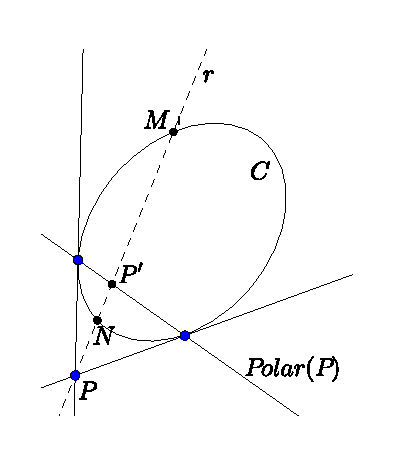
\includegraphics[scale=.8]{Graficos/Conicas/Polar}
\end{center}
\begin{defi}
	Sea una cónica, un punto $P$ y $r$ una recta perteneciente al haz de base $P$. Sean $M$ y $N$ los puntos de corte de la recta $r$ con la cónica. Se define \ti{recta polar del punto $P$} al conjunto de puntos $P'$ que son el cuarto armónico de $P$ respecto al par $(M,N)$, y que se obtienen al variar $r$.
\end{defi}
\begin{defi}
	Sea una recta $r$ la recta polar de un punto $P$, entonces $P$ es el \ti{polo} de $r$.
\end{defi}

La recta polar del punto $P$ respecto a una cónica se denota Polar($P$). Equivalentemente, se podría decir que la recta Polar(P) está formada por los puntos $P'$ tales que el par $(P,P')$ separa armónicamente al par $(M,N)$, donde $M$ y $N$ varían con $r$.\\

A partir de la definición determinemos la ecuación implícita de la recta polar de un punto $P$. Aunque la definición es válida para cualquier punto $P$, ya esté en la cónica, sea exterior a ella o interior, comenzaremos tomando un punto $P$ que se encuentre \tb{fuera de la cónica}. 

Así pues, sea $\mc{C}$ una cónica, cuya ecuación viene dada por
\begin{equation}
X^tAX=0,
\end{equation}
y un punto $P$ exterior a $\mc{C}$. Sea una recta arbitraria $r$ del haz de base $P$ tal que $r\cap \mc{C}=\{M,N\}$, con $M$ y $N$ distintos. Buscamos los puntos $P'$ tales que $\{M,N;P,P'\}=-1$. Por tanto, $P'$ debe estar en la recta $r$. Parametrizamos la recta $r$, tomando representantes de los puntos $P=[\vec{p}]$ y $P'=[\vec{p}']$:
\begin{equation*}
	r:[\vec{p}+\theta \vec{p}']
\end{equation*}
De esta forma podemos escribir
\begin{equation*}
	M=[\vec{p}+\theta_M \vec{p}'] \ , \quad N=[\vec{p}+\theta_N \vec{p}'] \ , \quad P=0 \ , \quad P'=\infty \ ,
\end{equation*}
donde $\theta_M$ y $\theta_N$ son las coordenadas no homogéneas de los puntos de corte $M$ y $N$, y $P$ y $P'$ se expresan en coordenadas no homogéneas.

Por tanto, 
\begin{equation}
-1=\{M,N;P,P'\}=\{\theta_M,\theta_N;0,\infty\}\Leftrightarrow \theta_M=-\theta_N
\end{equation}
Tenemos así una restricción para los puntos $M$ y $N$. Recordemos que además son la intersección de la recta $r$ con la cónica $\mc{C}$. Los puntos de corte viene dados por la ecuación
\begin{equation}
(\vec{P}+\theta \vec{P}')^tA(\vec{P}+\theta \vec{P}')=\vec{P}^tA\vec{P}+2\theta \vec{P}^tA\vec{P}'+\theta^2\vec{P}'^tA\vec{P}'=0
\end{equation}
que se obtiene simplemente de sustituir la ecuación paramétrica de $r$, donde $\vec{P}$ son vectores columna, en la ecuación de la cónica (cosa que ya hemos hecho antes varias veces). Recibe el nombre de \textbf{ecuación de Joachimstal} y nos permite calcular la intersección de una cónica y una recta.

Dado que en este caso la intersección son los puntos $M$ y $N$, las soluciones a esta ecuación deben ser $\theta_N$ y $\theta_M=-\theta_N$. Una ecuación de segundo grado tiene soluciones iguales y de signo opuesto si y solo si el término de grado uno es nulo. Por tanto, necesariamente
\begin{equation}\label{C8_eq_puntos_recta_polar}
\vec{P}^tA\vec{P}'=0
\end{equation}
Por ende, los puntos $P'$ buscados deben cumplir esta ecuación. Cuando se cumple esta ecuación se dice que \ti{$P'$ es conjugado de $P$ respecto a la cónica}. Por tanto, los puntos de la recta Polar($P$) son conjugados de $P$ respecto a la cónica.

El punto $P$ y la matriz $A$ son conocidos, por tanto, el producto $\vec{P}^tA$ dará como resultado el vector $u=(u_1, u_2,u_3)$ conocido. El punto $P'$ es desconocido, pudiéndolo escribir como $(x, y,z)$. De esta forma, los puntos $P'$ de la recta Polar(P) deben cumplir
\begin{equation}
(u_1 \ u_2 \ u_3)
\left( \begin{array}{c}
x\\ y\\ z
\end{array}\right) =0
\end{equation}
Notemos que esto es la ecuación de una recta con coeficientes $u_1,u_2$ y $u_3$. Dado que los puntos que cumplen la ecuación son los $P'$, esta no es otra que la ecuación implícita de la recta polar del punto $P$ respecto a la cónica $\mc{C}$.

Es decir, los coeficientes de la recta Polar(P) vienen dados por
\begin{equation}
u=\vec{P}^tA\Rightarrow u^t=A\vec{P}
\end{equation}
Si el punto $P$ fuese \tb{interior a la cónica}, los puntos de corte de las rectas del haz con base $P$ y la cónica $\mc{C}$ serían puntos imaginarios conjugados.
\begin{obs}
	Si $l_0$ es la recta polar del punto $P$, es decir, si $P$ es el polo de $l_0$, entonces $P=A^*l_0$.
\end{obs}
\begin{obs}
	Conviene recordar la notación utilizada en este apartado, pues será usada en ocasiones de aquí en adelante. En concreto, $P$ es un punto proyectivo tal que $P=[\vec{p}]$ y $\vec{P}$ es el vector columna de $\vec{p}$.
\end{obs}

\begin{obs}
	El punto $P'$ pertenece a la recta polar de $P\Leftrightarrow  \vec{P}^tA\vec{P}'=0\Leftrightarrow \vec{P}'^tA\vec{P}=0\Leftrightarrow $ el punto $P$ pertenece a la recta polar de $P'$.
\end{obs}

Por tanto, dada una cónica, un punto $P$ exterior a la cónica y un punto $P'$ perteneciente a la recta Polar(P), si trazamos una recta que pasa por $P'$ y que corta a la cónica en dos puntos $M$ y $N$ y encontramos el cuarto armónico $Q$ de $P'$ respecto a $(M,N)$, la recta polar de $P'$ será aquella que pase por $Q$ y $P$ (pues al pertenecer $P'$ a la recta polar de $P$, $P$ pertenece a la recta polar de $P'$). Observamos que se encuentra fuera de la cónica. Esto es coherente con que los puntos de corte de Polar(P') con la cónica sean imaginarios, ya que $P'$ es un punto interior a la cónica.
\begin{center}
	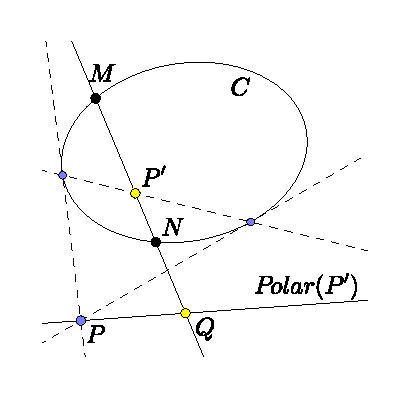
\includegraphics[scale=.8]{Graficos/Conicas/PolarInterior}
\end{center}

\tb{Construcción geométrica:} Hagamos ahora una construcción geométrica de la recta Polar(P) (mostrada en la siguiente figura). Para poder trazar esta recta debemos encontrar dos puntos que pertenezcan a ella, es decir, dos cuartos armónicos.
\begin{center}
	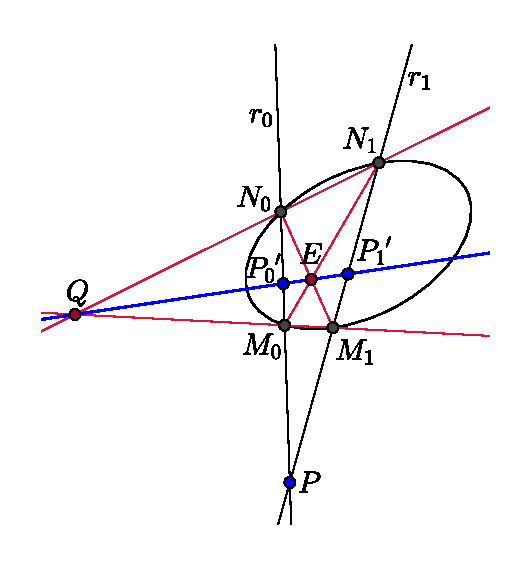
\includegraphics[scale=.8]{Graficos/Conicas/ConstruccionPolar}
\end{center}
Tomamos dos rectas $r_0$ y $r_1$ del $\haz_P$ que cortan con la cónica en los puntos $M_0$, $N_0$ y $M_1$, $N_1$, respectivamente. El cuarto armónico $P_0'$ de $P$ respecto del par $(M_0,N_0)$ pertenece a la recta Polar(P), al igual que el cuarto armónico $P_1'$ de $P$ respecto del par $(M_1,N_1)$. Tenemos así dos puntos que pertenecen a la recta polar del punto $P$.

Para encontrar los puntos $P_0'$ y $P_1'$ procedemos de la siguiente manera. Se recomienda ir dibujándolo mientras se explica para entender el proceso. Si se siguen los pasos indicados, la figura resultante debe ser equivalente a la figura anterior.

Trazamos la recta que pasa por $N_0$ y $M_1$ y la que pasa por $N_1$ y $M_0$, las cuales se cortan en un punto $E$. De la misma forma, la recta que pasa por $N_0$ y $N_1$ y la que pasa por $M_0$ y $M_1$ se cortan en un punto $Q$. Finalmente, la recta que pasa por $Q$ y por $E$ es la recta Polar(P), que corta con $r_0$ y $r_1$ en los puntos $P_0'$ y $P_1'$.

Podríamos preguntarnos por qué la recta $QE$ es la recta polar, ya que lo hemos asegurado sin explicar nada. Obsérvese que lo único que hemos hecho ha sido la construcción geométrica de un cuadrilátero completo para los puntos $P,M_0,N_0$ y el punto de corte de $QE$ con $r_0$ ($P_0'$), y otro para los puntos $P,M_1,N_1$ y el punto de corte de $QE$ con $r_1$ ($P_1'$). Esto asegura que los puntos están separados armónicamente. Por tanto, necesariamente, la recta $QE$ es la recta polar, pues los puntos que pertenecen a ella son los $P'_i$ tales que $(P,P'_i)$ están separados armónicamente de $(M_i,N_i)$.\\

Al principio de esta sección se mostró una construcción geométrica y en ella se indicó la recta polar de un punto $P$. Para ver que, efectivamente, esa es la recta polar es necesario avanzar un poco más. Con ese fin, damos la siguiente definición.

\begin{defi}
	Una recta es \ti{tangente} a una cónica si la corta en un punto con multiplicidad mayor que uno.
\end{defi}
\begin{lem}
	Sea $r$ la recta polar de un punto $P$ respecto a una cónica $\mc{C}$, con matriz $A$. Entonces, las rectas $PP_i'$ con $i=0,1$, donde $P_i'$ son los puntos de corte de la recta polar con la cónica, son tangentes a $\mc{C}$.
\end{lem}
\begin{proof}
	La recta $PP_0'$ tiene como ecuación paramétrica
	\begin{equation*}
		[\vec{p}+\theta\vec{p_0}']
	\end{equation*}
	Para ver que es tangente a la cónica debemos comprobar que $P_0'$ es un punto de corte de multiplicidad mayor que uno. Para ello, escribimos la ecuación de Joachimstal correspondiente a la intersección de $PP_0$ con la cónica, tomando vectores columna:
	\begin{equation}
	(\vec{P}+\theta \vec{P}')^tA(\vec{P}+\theta \vec{P}')=\vec{P}^tA\vec{P}+2\theta \vec{P}^tA\vec{P}'+\theta^2\vec{P}'^tA\vec{P}'=0
	\end{equation}
	El segundo sumando se anula por pertenecer $P_0'$ a la recta polar de $P$ (ecuación~\eqref{C8_eq_puntos_recta_polar}). El tercero también es nulo, ya que $P_0'$ pertenece a la cónica. La ecuación se reduce a 
	\begin{equation}
	\vec{P}^tA\vec{P}=0
	\end{equation}
	Recordemos que esta era una ecuación de segundo grado con solución doble $\theta=\infty$. Por tanto, el punto de corte de la recta $PP_0'$ con la cónica, que es $[\vec{p}+\infty\vec{p_0}']=P_0'$, es doble, por lo que su multiplicidad es mayor que uno. Se conlcuye así que la recta $PP_0'$ es tangente a la cónica. De forma análoga $PP_1'$ es tangente a $\mc{C}$.
\end{proof}

\begin{obs}
	Podemos definir una recta tangente a una cónica como aquella cuya ecuación de Joachimstal, de la intersección de la recta con la cónica, tiene solución doble.
\end{obs}

Gracias al lema anterior, si demostrásemos que, desde un punto $P$ exterior a la cónica, se pueden trazar siempre dos únicas rectas tangentes, entonces quedaría demostrado que la recta generada por los puntos de corte de esas tangentes con la cónica es la recta polar del punto $P$. Con ello, la construcción inicial quedaría justificada.
\begin{obs}
	Esta última construcción puede verse como un caso límite de la anterior cuando acercamos los puntos $N_0$ y $N_1$ entre sí y los puntos $M_0$ y $M_1$ entre sí (o bien los puntos $N_0$ y $M_0$ por un lado, y los puntos $M_1$ y $N_1$ por otro).
\end{obs}

Nos queda por último hablar de la recta polar de un punto \tb{perteneciente a la cónica} no degenerada $\mc{C}$. Aunque dedujimos que los coeficientes de la recta Polar($Q$) eran $AQ$ (donde $A$ es la matriz de la cónica) suponiendo que $Q$ era un punto exterior a la cónica, tomaremos esto como válido también para puntos de la cónica. Es importante recalcar que en este caso no tenemos la propiedad de la cuaterna armónica.

Por tanto, dado un punto $P\in \mc{C}$, los coeficientes de la recta Polar($P$) son $AP$. Veamos que consecuencias tiene esto.

\begin{lem}
	Sea una cónica $\mc{C}$ no degenerada, con matriz $A$, y un punto $P=\class{\vec{p}}\in \mc{C}$, entonces la recta Polar($P$) es tangente a la cónica.
\end{lem}
\begin{proof}
	Para demostrar que es una recta tangente veamos que la ecuación de Joachimstal tiene solución doble.
	
	Sea $Q=\class{\vec{q}}$ un punto de la recta Polar($P$). Entonces, dicha recta puede parametrizarse como 
	\[\text{Polar($P$)}=\{\class{\vec{p}+\theta\vec{q}}\tq\theta\in\overline{\K}\}\]
	Recordemos además que todo punto perteneciente a la polar de $P$ es conjugado de $P$ respecto a la cónica.
	
	La ecuación de Joachimstal queda
	\begin{equation*}
	(\vec{P}+\theta \vec{Q})^tA(\vec{P}+\theta \vec{Q})=\vec{P}^tA\vec{P}+2\theta \vec{P}^tA\vec{Q}+\theta^2\vec{Q}^tA\vec{Q}=0
	\end{equation*}
	El primer sumando es nulo por pertenecer $P$ a la cónica y el segundo por ser $Q$ conjugado de $P$ respecto a $\mc{C}$. Queda entonces la ecuación
	\[\theta^2\vec{Q}^tA\vec{Q}=0\]
	que tiene $\theta=0$ como solución doble.
\end{proof}
\begin{obs}
	Dado un punto $P$ exterior a la cónica, recordemos que si $R$ está en la recta polar de $P$, entonces $P$ está en la recta polar de $R$. Si $R$ pertenece a la cónica, entonces Polar($R$) es tangente a la cónica, por lo que $PR$ es tangente a la cónica.
\end{obs}

Por último, veamos lo prometido, que desde un punto exterior a la cónica se puden trazar siempre dos únicas rectas tangentes. Para ello veamos que las rectas que pasan por un punto $P$ exterior a la cónica y son tangentes a la misma forman una cónica degenerada.

Sea entonces una recta $PQ$ tangente a la cónica, que se puede parametrizar como 
\[PQ:\{\class{\vec{p}+\theta\vec{q}}\tq\theta\in\overline{\K}\}\]
Por ser tangente, la ecuación de Joachimstal
\[(\vec{P}+\theta \vec{Q})^tA(\vec{P}+\theta \vec{Q})=0\]
debe tener solución doble. Esto ocurre si y solo si el discriminante es nulo, es decir, si y solo si
\[(2\vec{P}^tA\vec{Q})^2-4(\vec{P}^tA\vec{P})(\vec{Q}^tA\vec{Q})=0\]
\[(\vec{P}^tA\vec{Q})^2-(\vec{P}^tA\vec{P})(\vec{Q}^tA\vec{Q})=0\]
Si escribimos $\vec{q}=(x,y,z)$ el resultado de la ecuación anterior es una ecuación de segundo grado en $x,y,z$, que es la ecuación de la cónica degenerada formada por las rectas tangentes a $\mc{C}$. Desarrollémoslo para obtener también la matriz de dicha cónica. Por sencillez, renombremos $\vec{q}=\vec{x}=(x,y,z)$.
\[(\vec{P}^tA\vec{X})^2-(\vec{P}^tA\vec{P})(\vec{X}^tA\vec{X})=0\]
\[\vec{X}^tA\vec{P}\vec{P}^tA\vec{X}-\vec{X}^t(\vec{P}^tA\vec{P})A\vec{X}=0\]
Por tanto, la ecuación de la \tb{cónica formada por las rectas tangentes} a la cónica que pasan por el punto $P$ es
\begin{equation}
	\vec{X}^t(A\vec{P}\vec{P}^tA-\vec{P}^tA\vec{P}A)\vec{X}=0
\end{equation}
siendo así su matriz
\begin{equation}
\overline{A}=A\vec{P}\vec{P}^tA-\vec{P}^tA\vec{P}A
\end{equation}

\section{Cónicas Duales}
Sea una cónica no degenerada $\mc{C}$ y un punto $X\in \mc{C}$. Sabemos que la recta tangente a $\mc{C}$ en el punto $X$ es la polar de $X$. Por tanto, tiene coeficientes $u=AX$. Podemos escribir entonces el punto $X$ como $X=A^{-1}u$. Como $X$ pertenece a la cónica cumple su ecuación, es decir
\[X^tAX=0\]
Por tanto,
\[(A^{-1}u)^tA(A^{-1}u)=0\sii u^tA^{-1}u=0\]
Dado que $u$ son los coeficientes de una recta, en el dual son las coordenadas de un punto. Por ello, la ecuación anterior define una cónica en el dual, que denominaremos cónica dual. Dado que $A^{-1}$ y $A^*$ son proporcionales, la ecuación de la cónica dual se puede escribir como
\begin{equation}\label{C8_eq_conicadual}
	u^tA^*u=0
\end{equation}
Nótese que cualquier recta tangente a la cónica $\mc{C}$ satisface la ecuación anterior, pues $X$ es arbitrario.

Recíprocamente, si una recta $u$ satisface la ecuación de la cónica dual, entonces es tangente a $\mc{C}$. En efecto, sean $u$ los coeficientes de una recta que pertenece a la cónica dual, podemos definir $X=A^*u\sii u=AX$, siendo entonces esta la recta tangente a $\mc{C}$ en $X$ siempre que $X\in \mc{C}$. Pero, efectivamente, $X$ pertenece a la cónica pues
\[X^tAX=(A^*u)^tAA^*c=u^tA^*u=0\] 
Podemos pues introducir la siguiente definición.
\begin{defi}[Cónica dual asociada a una cónica no degenerada]
	Dada una cónica no degenerada $\mc{C}$, las rectas tangentes a $\mc{C}$ son una cónica de rectas en el dual denominada \ti{cónica dual}, la cual denotaremos por $\mc{C}^*$.
\end{defi}
\begin{center}
	
\includegraphics[scale=.45]{Graficos/Conicas/ConicaDual.JPG}
\end{center}
Veamos un ejemplo
\begin{exa}[Cónica Dual]
	Sea $\mc{C}:Y-X^2=0$ una cónica no degenerada. Hallar la ecuación de la cónica dual y la expresión de una recta tangente a $\mc{C}$ arbitraria.\\
	
	Primero, homogeneizamos la cónica, obteniendo $\mc{C}:yz-x^2=0$. La matriz de la cónica es
	\[A=\left( \begin{array}{ccc}
		2&0&0\\
		0&0&-1\\
		0&-1&0
	\end{array}\right) \]
	Calculamos su adjunta
	\[A^*=\left( \begin{array}{ccc}
		 -1&0&0\\
		 0&0&2\\
		 0&2&0
	\end{array}\right) \]
	La ecuación de la cónica dual $C^*$ será 
	\[\mc{C}^*:\left( \begin{array}{ccc}
	u&v&w
	\end{array}\right) A^*\left( \begin{array}{c}
	u\\v\\w
	\end{array}\right) =0\sii\mc{C}^*:-u^2+4vw=0\]
	Por tanto, $C^*$ está formada por rectas $ux+vy+wz=0$ cuyos coeficientes cumplen la relación
	\[u^2=4vw\sii \left( \frac{u}{w}\right) ^2=4\frac{v}{w}\]
	Dado que estas rectas son las rectas tangentes a $C$, deshomogeneizando podemos escribir las mismas como
	\[ux+vy+wz=0\sii \frac{u}{w}x+\frac{v}{w}y+z=0\sii Ux+\frac{U^2}{4}y+1=0\]
	donde $U=\frac{u}{w}$. 
	
	Comprobemos que, efectivamente, las rectas tangentes a $\mc{C}$ son de esa forma. Un punto arbitrario de la cónica $\mc{C}$ podemos escribirlos como $(X,Y)=(X,X^2)$. Calculamos la recta tangente como sabemos desde primero, utilizando derivadas. Teniendo en cuenta que $Y'=2X$, la tangente en el punto $(X_0,Y_0)=(X_0,X_0^2)$ queda
	\[Y-Y_0-2X_0(x-x_0)=0\sii Y-X_0^2=2X_0(X-X_0)=0\sii\]
	\[-2X_0X+Y+X_0^2=0\sii -\frac{2}{X_0}X+\frac{1}{X_0^2}Y +1=0\]
	Efectivamente, como $-\frac{2}{X_0}=U$, se cumple que $V=\frac{1}{X_0^2}=\frac{U^2}{4}$.
\end{exa}
\subsection{Cónicas duales degeneradas}
Sería insatisfactorio que el concepto de cónica dual solo estuviese definido para cónicas no degeneradas. Por suerte, no es así. Dado que las cónicas degeneradas pueden tener matrices de rango $1$ o $2$, distingamos ambos casos.\\

Sea $\mc{C}$ una cónica degenerada tal que el rango de su matriz $A$ es $2$. Entonces, será una cónica de la forma $\mc{C}:l m$ siendo $l,m$ dos rectas distintas. Es claro que las rectas tangentes a $\mc{C}$, aquellas que cortan con multiplicidad mayor que uno, son las que pasan por $l\cap m$. Por tanto, tendría sentido que la cónica dual, que hemos definido como el conjunto de las rectas tangentes a $\mc{C}$ fuese el haz de rectas con base $l\cap m$.

Veamos que si $X_0=(a_0:b_0:c_0)$ es el punto de corte de ambas rectas, entonces $\haz_{X_0}$ es una cónica dual y que, en efecto, es la cónica dual asociada a $\mc{C}:l m$.

Recordemos del tema $3$ que el $\haz_{X_0}$ es la recta de $\proy^{2*}$ con ecuación implícita $a_0u+b_0v+c_0w=0$. Para no perdernos, con $p^*$ nos referiremos a la recta $\haz_{X_0}$ del dual. El haz y $p^*$ son lo mismo, pero para saber donde estamos trabajando, si es en $\proy^2$ o $\proy^{2*}$, tomaremos notaciones diferentes.

La recta $p^*$ podemos verla como la cónica dual degenerada de ecuación $(p^*)^2=(a_0u+b_0v+c_0w)^2=0$. Escribámoslo matricialmente. Siendo 
\[X_0=\left( \begin{array}{c}
a_0\\b_0\\c_0
\end{array}\right) ,\quad U=\left( \begin{array}{c}
u\\v\\w
\end{array}\right) \]
se tiene que la ecuación de la cónica dual degenerada es
\[(X_0^tU)^2=0\sii U^tX_0X_0^tU=0\]
Por tanto, el haz de rectas $\haz_{X_0}$ es una cónica dual degenerada cuya matriz es $A^*=X_0X_0^t$.

Nos queda comprobar que es la cónica dual asociada a $\mc{C}:lm$. Para ello tendríamos que demostrar que la matriz de $\mc{C}$ es $A$.

Como $X_0=l\cap m$, y recordando del tema $3$, si $u,v$ son los coeficientes de las rectas $l$ y $m$, respectivamente, podemos escribir $X_0=(u\times v)$, donde $\times$ denota el producto vectorial. Así, la matriz de la cónica dual puede escribirse como
\begin{equation}
	A^*=-(u\times v)(u\times v)^t
\end{equation}
Si retomamos el ejercicio $91$ de los problemas de geometría lineal podemos asegurar la siguiente igualdad
\begin{equation}
	A^*=-(u\times v)(u\times v)^t=(uv^t+vu^t)^*
\end{equation}
Por otro lado, en la sección~\ref{C8_subsec_producto_rectas} vimos que la matriz de la cónica $\mc{C}$ es precisamente $uv^t+vu^t$. Por tanto, queda comprobado que la matriz de la cónica dual es la adjunta de la matriz de $\mc{C}$.

Así, $\mc{C}^*=\haz_{X_0}$ sigue siendo la cónica dual asociada a $\mc{C}$ que me proporciona todas las rectas tangentes a la misma y cuya matriz es $A^*$.\\

Vayamos con el otro caso. Sea $\mc{C}$ una cónica degenerada tal que el rango de su matriz $A$ es $1$. Entonces, será una cónica de la forma $\mc{C}:l^2$. Las rectas tangentes a $\mc{C}$, aquellas con multiplicidad en el corte mayor que uno, son todas las rectas del plano proyectivo. Por tanto,la ecuación
\[u^tA^*u=0\]
debe cumplirse para cualquier recta de coeficientes $u$. Esto ocurre si y solo si $A^*$ es la matriz nula. Dado que $rg(A)=1$ todas las submatrices de orden $2$ de $A$ tienen determinante nulo. Por tanto, de nuevo, podemos asegurar que la cónica dual asociada a $\mc{C}$ nos proporciona todas las rectas tangentes a la misma y tiene por matriz $A^*$.\\

Resumamos todo esto en una definición.
\begin{defi}[Cónica dual asociada a una cónica degenerada]
	Sea $\mc{C}$ una cónica degenerada con matriz $A$, las rectas tangentes a $\mc{C}$ son una cónica de rectas en el dual. Esto implica que, si $\mc{C}:lm$, la cónica dual asociada es $\haz_{l\cap m}$ con matriz $A^*$. Por otro laso si $\mc{C}:l^2$, la cónica dual asociada son todas las rectas del plano.
\end{defi}
\begin{obs}
	Es importante observar que en el caso de las cónicas degeneradas la cónica dual de la cónica dual no se identifica con la cónica inicial.
\end{obs}

\section{Parametrización de cónicas}
Existen diversas formas de parametrizar cónicas no degeneradas. Sin embargo, hay una de ellas que resulta especialmente útil, pues nos permite parametrizar cualquier cónica no degenerada como una parábola. Comenzaremos con ella.
\subsection{Parametrización de cónicas como parábolas}
\label{C8_subsec_parametrizacion_como_parabola}
Recordemos que, al hablar de cónicas y cambios de referencia, pusimos la mano en el fuego al intuir que, con un cambio de referencia adecuado, podríamos trasformar una cónica en cualquier otra (preservando la degeneración). Esta parametrización es una muestra de que, efectivamente, es posible. Desarrollémosla en detalle.\\

Dada una cónica no degenerada $\mc{C}$ en cierta referencia proyectiva, realizaremos un cambio de referencia de tal forma que, la ecuación de la cónica en la referencia final, sea la ecuación de una parábola. De esta forma, bastará con parametrizar una parábola para obtener la parametrización de cualquier cónica no degenerada.

Para ello, tomemos dos puntos $X_0$ y $X_2$ de la cónica y escojamos $X_1$ como el punto de corte de las rectas tangentes a la cónica en $X_0$ y $X_2$. Nuestra referencia será $\mf{R}=\{X_0,X_1,X_2;e\}$, donde $e$ es un punto de la cónica distinto al resto.
\begin{center}
	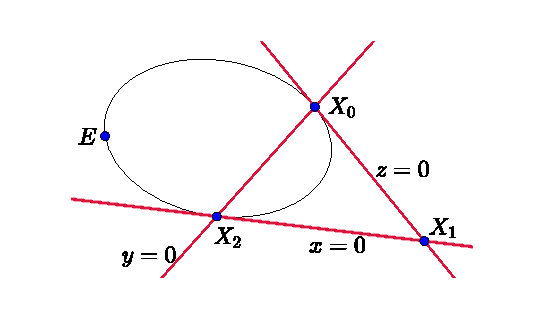
\includegraphics[scale=.9]{Graficos/Conicas/Parametrizacionparabola}
\end{center}
Hallemos la matriz de la cónica resultante de realizar este cambio de referencia. Esta matriz será de la forma
\begin{equation*}
	A=\left( \begin{array}{ccc}
	a & h & g\\
	h & b & f\\
	g & f & c
	\end{array}\right) 
\end{equation*}
Como $X_0\in \mc{C}$, debe cumplir la ecuación de la cónica en la nueva referencia. Dado que en esta referencia $X_0=(1:0:0)$, debe cumplirse la siguiente ecuación:
\begin{equation*}
	\begin{pmatrix}
		1 & 0 & 0
	\end{pmatrix}A 
	\left( \begin{array}{c}
		1\\0\\0
	\end{array}\right) =0\sii a=0
\end{equation*}
Realizando la misma operación para el punto $X_2=(0:0:1)$ se tiene que $X_2\in \mc{C}\sii c=0$. Con ello, la matriz de la cónica queda
\begin{equation*}
	A=\left( \begin{array}{ccc}
		0 & h & g\\
		h & b & f\\
		g & f & 0
	\end{array}\right) 
\end{equation*}
Por otro lado, con la elección de puntos que hemos hecho, la recta $X_0X_2$ es la recta polar de $X_1$. Por tanto, la ecuación implícita de ambas rectas debe coincidir, salvo factor de proporcionalidad. La ecuación implícita en la referencia $\mf{R}$ de la recta $X_0X_2$ es conocida 
\begin{equation*}
	X_0X_2:
	\begin{pmatrix}
		0 & 1& 0
	\end{pmatrix}
	\left( \begin{array}{c}
		x\\y\\z
	\end{array}\right)=0
\end{equation*}

Recordemos que la ecuación implícita de la recta polar que pasa por un punto $P$ es
\begin{equation*}
	u\left( \begin{array}{c}
	x\\y\\z
	\end{array}\right)=
	\begin{pmatrix}
	u_1 & u_2 & u_3
	\end{pmatrix}
	\left( \begin{array}{c}
	x\\y\\z
	\end{array}\right)=0
\end{equation*}
donde los coeficientes de la recta vienen dados por 
\begin{equation*}
	u^t=A\vec{P}
\end{equation*}
En nuestro caso
\begin{equation*}
u^t=A\vec{X}_1=A\left( \begin{array}{c}
	0\\1\\0
\end{array}\right)
\end{equation*}
Igualando los coeficientes de las ecuaciones implícitas se tiene que
\begin{equation*}
	A\left( \begin{array}{c}
	0\\1\\0
	\end{array}\right)=\rho \left( \begin{array}{c}
	0\\1\\0
	\end{array}\right)\sii h=0, \ f=0
\end{equation*}
Finalmente, la matriz de nuestra cónica en la referencia $\mf{R}$ es
\begin{equation*}
	A=\left( \begin{array}{ccc}
		0 & 0 & g\\
		0 & b & 0\\
		g & 0 & 0
	\end{array}\right) \sim 
	\left( \begin{array}{ccc}
		0 & 0 & 1\\
		0 & k & 0\\
		1 & 0 & 0
	\end{array}\right) \tq k=\frac{b}{g}
\end{equation*}
Si escribimos la ecuación de la cónica en esta referencia, a partir de la matriz A, obtendremos
\begin{equation*}
	ky^2=-2xz
\end{equation*}
Esta ya es la ecuación de una parábola. Sin embargo, podemos ir más allá. Nuestro punto unidad ha sido olvidado, pero recordemos que lo escogimos de tal forma que perteneciese a la cónica. Por tanto, $(1:1:1)\in \mc{C}$. Sustituyéndolo en la ecuación anterior obtenemos que $k=-2$. Así, la ecuación de la cónica, en la referencia proyectiva $\mf{R}$, es
\begin{equation}
	y^2=xz
\end{equation}
Deshomogeneizando se transforma en 
\begin{equation}
	Y^2=X \tq Y=\frac{y}{z}, \ X=\frac{x}{z}
\end{equation}
Por tanto, tomando la referencia indicada, cualquier cónica no degenerada es la parábola $y^2=xz$. Nótese la importancia de este hecho. Esto implica que, una vez que tengamos parametrizada la parábola $y^2=x$, tendremos parametrizada cualquier cónica no degenerada en la referencia $\mf{R}$ adecuada. Para obtener la parametrización en la referencia inicial (aquella en la que la cónica no era una parábola) bastará con cambiar de referencia la parametrización de la parábola.

Y, ¡oh, dioses benévolos!, parametrizar una parábola es extremadamente sencillo. Si elegimos el plano $z=1$ como representante afín, la parábola $y^2=xz$ consta de los puntos proyectivos $(\theta^2:\theta:1)$, para $\theta\in \overline{\K}$. Observemos que el punto correspondiente a $\theta=\infty$ es el $(1:0:0)$.

Veremos a continuación un ejemplo concreto, pero antes, una pequeña observación.
\begin{obs}
	Aunque se ha desmostado matricialmente que, escogiendo la referencia $\mf{R}=\{X_0,X_1,X_2;e\}$ correspondiente, cualquier cónica no degenerada se trasforma en la parábola $Y^2=X$, puede deducirse directamente de esta elección. Dado que puede resultar poco obvio, se decidió plantear primero la solución matricial. A continuación daremos una idea de como deducirlo.\\
	
	Teniendo en cuenta los puntos de la referencia, las rectas tangentes a la cónica que pasan por $X_1$, es decir, las rectas $X_0X_1$ y $X_2X_1$, son las rectas $z=0$ y $x=0$ respectivamente. Si tomamos $z=0$ como la recta del infinito, nuestra cónica es tangente al infinito. Atendiendo a la clasificación de cónicas no degeneradas, se trata de una parábola. También es tangente a la recta $x=0$, por lo que tiene que ser una parábola de la forma
	\begin{center}
		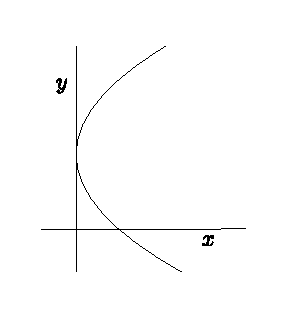
\includegraphics[scale=.6]{Graficos/Conicas/Parabola2}
	\end{center}
	Por último, pasa por el punto $X_2$, que se corresponde al punto $(X,Y)=(0,0)$, y por el punto $e$, que se corresponde a $(X,Y)=(1,1)$. Por tanto, no tiene más remedio que ser la cónica $Y^2=X$
	\begin{center}
		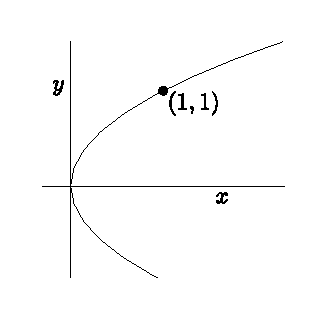
\includegraphics[scale=.6]{Graficos/Conicas/Parabola3}
	\end{center}
\end{obs}
Vayamos con el ejemplo prometido.
\begin{exa}[Parametrización de cónicas]\label{C8_exa_parametrizacion_parabola}
	Parametrizar la cónica dada por la siguiente ecuación:
	\begin{equation}
		\mc{C}:4x^2+xy+y^2-23xz-5yz+30z^2=0
	\end{equation}
	La matriz de la cónica es 
	\begin{equation*}
	A=\left( \begin{array}{rrr}
	4& 1/2 & -23/2\\
	 1/2 & 1 & -5/2\\
	-23/2 & -5/2 & 30
	\end{array}\right) 
	\end{equation*}
	Para parametrizarla tomemos la referencia que nos permite expresar esta cónica como una parábola y realicemos el cambio de referencia proyectiva.
	
	Escogemos pues, dos punto de la cónica $X_0=(2:3:1)$ y $X_2=(3:-1:1)$. El punto $X_1$ es el polo de la recta $X_0X_2$. Dado que esta recta viene dada por la ecuación $4x+y-11z=0$, y que los coeficientes de la recta polar de $X_1$ vienen dados por $A\vec{X}_1$, se tiene que
	\begin{equation*}
		A\vec{X}_1=\rho \left( \begin{array}{c}
		4\\1\\-11
		\end{array}\right)\sii \rho'\vec{X}_1=A^{-1}
		\left( \begin{array}{c}
			4\\1\\-11
		\end{array}\right)
	\end{equation*}
	Realizando los cálculos se obtiene $X_1=(-1:-1:1)$. Por último, tomemos un punto unidad que pertenezca a la cónica, distinto de los anteriores. Por ejemplo, $e=(2:0:1)$.
	
	Nuestra referencia final será
	\[\mf{R}=\{X_0,X_1,X_2;e\}=\{(2:3:1),(-1:-1:1),(3:-1:1);(2:0:1)\}\]
	cuya base asociada es $\mc{B}=\{(8,12,4),(-3,-3,3),(27,-3,3)\}=\{4\vec{x}_0,3\vec{x}_1,9\vec{x}_2\}$. Por tanto, la matriz de cambio de referencia es
	\begin{equation*}
		M=\left( \begin{array}{ccc}
			8&-3&27\\
			12&-3 &-9\\
			4&3&9
		\end{array}\right) 
	\end{equation*}
	Gracias a la elección de $\mf{R}$ sabemos que la matriz de la cónica $\overline{A}$ en esta referencia será la matriz de la parábola $y^2=xz$. Si queremos asegurarnos, solo hay que aplicar la ecuación~\eqref{C8_eq_relacionMatrices_referencias}, según la cual
	\begin{equation*}
		\overline{A}=M^tAM=
		\left( \begin{array}{ccc}
		0 & 0 & -1\\
		0 & 2 & 0\\
		-1 & 0 & 0
		\end{array}\right)
	\end{equation*}
	Por tanto, la parametrización de la cónica $\mc{C}$ en la referencia $\mf{R}$ es 
	\begin{equation*}
	 \mc{C}=\{(\theta^2:\theta:1)\tq \theta\in\overline{\K}\}
	\end{equation*}
	Para parametrizar $\mc{C}$ en la referencia inicial solo es necesario realizar un cambio de coordenadas. Si $X$ son las coordenadas de un punto en la referencia inicial y $\overline{X}$ las coordenadas de un punto en la referencia $\mf{R}$, sabemos que se cumple
	\begin{equation*}
		\rho X=M\overline{X}
	\end{equation*}
	Por tanto, un punto genérico de la cónica en la referencia inicial será
	\begin{equation}
		X^t=(M\overline{X})^t=
		\begin{pmatrix}
		\theta^2 & \theta & 1
		\end{pmatrix}M^t=(8\theta^2-3\theta+27,12\theta^2-3\theta-9,4\theta^2+3\theta+9)
	\end{equation}
	Finalmente, la parametrización de la cónica $\mc{C}$ pedida es
	\begin{equation*}
		\mc{C}=\{(8\theta^2-3\theta+27,12\theta^2-3\theta-9,4\theta^2+3\theta+9)\tq \theta\in\overline{\K}\}
	\end{equation*}
\end{exa}
\begin{obs}[Una cónica es un $\proy^1$]
	Una vez que sabemos parametrizar cónicas es cuestión de segundos darnos cuenta de que estamos tratando la cónica como un $\proy^1$. En efecto, consideramos la referencia utilizada durante toda esta sección, $\mf{R}=\{X_0,X_1,X_2;e\}$ con $X_0,X_2,e\in \mc{C}$. La aplicación
	\[\begin{array}{cccc}
		h:& \mc{C}&\rightarrow &\proy^1\\
		&X&\rightarrow &\theta\\
		&X_0=\infty&\rightarrow &\infty\\
		&X_1=0&\rightarrow &0\\
		&e=1&\rightarrow &1\\
	\end{array}\]
	es la aplicación proyectiva identidad.
	
	Esto es realmente bello, ya que podremos definir en una cónica todo aquello que definíamos en un $\proy^1$: razón doble, homografías, involuciones, etc.
	
	Hay que tener cuidado y no confundirnos con la observación~\ref{C8_obs_conica_p5}. Cada cónica puede considerarse un $\proy^1$ y, a su vez, cada cónica es un punto en $\proy^5$.
\end{obs}
\begin{obs}
	Una vez que tenemos la cónica parametrizada, si queremos recuperar la matriz de la cónica, lo único que debemos hacer es obligar a la parametrización a cumplir la ecuación de la cónica y hallar así los coeficientes de la matriz.
\end{obs}

\subsection{Parametrización de cónicas y polinomios}
Un resultado inmediato de la sección anterior es el siguiente.
\begin{lem}
	\label{C8_lem_conicas_polinomios}
	Dada una cónica $\mc{C}$ en cierta referencia $\mf{R}$, esta puede parametrizarse como 
	\begin{equation}
	\label{C8_eq_parametrizacion_polinomios}
	\mc{C}=\{(p_1(\theta):p_2(\theta):p_3(\theta))\tq\theta\in\overline{\K}\}
	\end{equation}
	donde $p_1(\theta),p_2(\theta),p_3(\theta)$ son polinomios de grado menor o igual que 2 linealmente independientes.
	
	Recíprocamente, dados tres polinomios de grado menor o igual que 2 linealmente independientes, estos parametrizan una cónica.
\end{lem}
\begin{proof}
	Sea una cónica $\mc{C}$ en la referencia $\mf{R}$, veamos que puede parametrizarse como indica la ecuación~\eqref{C8_eq_parametrizacion_polinomios}. Si $\mc{C}$ es una parábola el resultado es trivial. Supongamos, por tanto, que, en dicha referencia, $\mc{C}$ no es una parábola. Tomemos entonces la referencia $\overline{\mf{R}}$ en la cual la cónica se parametriza como la parábola $y^2=xz$. Sea $M$ la matriz de cambio de la referencia $\overline{\mf{R}}$ a la referencia $\mf{R}$. Como vimos en el ejemplo~\ref{C8_exa_parametrizacion_parabola} , un punto genérico de la cónica en la referencia $\mf{R}$ puede escribirse como
	\begin{equation}
		X=M\overline{X}=M
		\left( \begin{array}{c}
		\theta^2\\\theta\\1
		\end{array}\right)
	\end{equation}
	Es claro que el vector $X$ estará formado por tres polinomios de grado menor o igual que 2:
	\[X=\left( \begin{array}{c}
	p_1(\theta)\\p_2(\theta)\\p_3(\theta)
	\end{array}\right)\]
	Además, los polinomios del vector $(\theta^2,\theta,1)$ son linealmente independientes y la matriz $M$ es invertible, y, por tanto, todas sus filas son linealmente independientes. Esto implica que $p_1(\theta),p_2(\theta),p_3(\theta)$ son linealmente independientes.\\
	
	Sean tres polinomios $p_1(\theta),p_2(\theta),p_3(\theta)$ de grado menor o igual que 2 linealmente independientes. Podemos escribir
	\begin{equation*}
		\left( \begin{array}{c}
		p_1(\theta)\\p_2(\theta)\\p_3(\theta)
		\end{array}\right)=H
		\left( \begin{array}{c}
		\theta^2\\\theta\\1
	\end{array}\right)
	\end{equation*}
	donde $H$ es la matriz de coeficientes. Como los polinomios son linealmente independientes, $H$ es invertible. Por tanto, podemos tomar $H$ como una matriz de cambio de referencia. Entonces, podemos considerar $(p_1(\theta):p_2(\theta):p_3(\theta))$ como la parametrización de la cónica $y^2=xz$ en cierta referencia (determinada por $H$). Queda así demostrado que
	$p_1(\theta),p_2(\theta),p_3(\theta)$ parametrizan una cónica.
\end{proof}
Por tanto, dada cualquier terna de polinomios de grado menor o igual que 2 linealmente independientes, existe una cónica, en cierta referencia, a la cuál parametrizan. Veamos un ejemplo.
\begin{exa}[Parametrización de cónicas por polinomios]
 	Dados los polinomios 
 	\[\begin{cases}
 		p_1(\theta)=\theta^2+\theta+1\\
 		p_2(\theta)=\theta-1\\
 		p_3(\theta)=\theta^2-5
 	\end{cases}\]
 	encuentra la cónica que engendran.\\
 	
 	Realizaremos los mismos pasos que se llevaron a cabo en la demostración del lema~\ref{C8_lem_conicas_polinomios}. Escribimos los polinomios dados matricialmente:
 	\begin{equation*}
 		\left( \begin{array}{c}
 			p_1(\theta)\\p_2(\theta)\\p_3(\theta)
 		\end{array}\right)=
 		\left( \begin{array}{ccc}
 			1&1&1\\
 			0&1&-1\\
 			1&0&-5
 		\end{array}\right) 
 		\left( \begin{array}{c}
 			\theta^2\\\theta\\1
 		\end{array}\right)=H
 		\left( \begin{array}{c}
 			\theta^2\\\theta\\1
 		\end{array}\right)
 	\end{equation*}
 	Consideramos el cambio de coordenadas $\rho \overline{X}=HX$. De esta forma $H$ es la matriz de paso de la referencia $\mf{R}$, en la cual la cónica es una parábola, a la referencia $\overline{\mf{R}}$, en la cual la cónica se parametriza por los polinomios dados. La matriz $A$ de la cónica en $\mf{R}$ es conocida, pues es la parábola $y^2=xz$. Recordado lo visto en el apartado de cónicas y cambio de referencia, la matriz de la cónica en la referencia $\overline{\mf{R}}$ es
 	\begin{equation}
	 	A=H^t\overline{A}H\sii \overline{A}=(H^t)^{-1}AH^{-1}
 	\end{equation}
 	Por tanto, la cónica engendrada por los polinomios dados es aquella cuya matriz asociada es
 	\begin{equation*}
	 	\overline{A}=\left( \begin{array}{ccc}
	 		-8&22&1\\
	 		22&62&-15\\
	 		1&-15&6
	 	\end{array}\right) 
 	\end{equation*}
\end{exa}
\subsection{Otras parametrizaciones}
Terminemos este apartado con una forma sencilla y rápida de parametrizar cónicas.\\

Escojamos un punto $X_0$ de la cónica y parametrizemos el haz de rectas $\haz_{X_0}$, escogiendo dos rectas del haz ($X_0X_1$ y $X_0X_2$) como base. Supongamos que las rectas $X_0X_1$ y $X_0X_2$ representan los puntos $(a_0:a_1:a_2)$ y $(b_0:b_1:b_2)$ en el dual, respectivamente. Entonces, la ecuación paramétrica del $\haz_{X_0}$ sería 
\[\haz_{X_0}=\{(a_0+\theta b_0:a_1+\theta b_1:a_2+\theta b_2)\tq \theta\in\overline{\K}\}\]
Cualquier recta del haz cortará a la cónica en dos puntos. Uno de ellos será $X_0$ y el otro un punto $P$ arbitrario. Queda excluida la recta del haz tangente a la cónica, pues solo corta en $X_0$. Por tanto, si cortamos una recta genérica del $\haz_{X_0}$ con la cónica, mediante la ecuación de Joachimstal, obtendremos la expresión de un punto arbitrario de la cónica, en función de $\theta$. Esto nos proporciona una parametrización de la cónica.

Es importante observar que, si escogemos otra base del haz de rectas, la parametrización resultante cambia.\\

Este procedimiento es rápido... siempre que no tenga que hacerse a mano. En ese caso, hay una forma de ``arreglar'' este método para que sea asequible. 

Una vez que tenemos nuestro haz $\haz_{X_0}$, con base un punto de la cónica, lo intersecamos con una recta cualquiera. Esto nos proporcionará un punto $P_\theta$ que dependerá de $\theta$, pues al cortar hemos utilizado una recta genérica del haz. Una vez que hemos conseguido este punto hallamos la ecuación paramétrica de la recta $X_0P_\theta=\{\class{\vec{x}_0+\mu \vec{p}_\theta}\tq \mu,\theta\in\overline{\K}\}$. Esta recta cortará en un punto, distinto de $X_0$, a la cónica. Aprovechando que tenemos la ecuación paramétrica de $X_0P_\theta$, al intersecarla con la cónica, cogemos la ecuación implícita de esta última. Obtendremos así un valor concreto para $\mu$. Esto nos proporcionará una parametrización de la cónica. De este modo, el cálculo es mucho más asequible si se va a realizar a mano.
\section{Teorema de Steiner}
A continuación expondremos un resultado que relaciona cónicas y homografías entre haces de rectas.
\begin{theo}[Teorema de Steiner]
	\label{C8_teo_steiner}
	Dada una homografía $h:\haz_A\rightarrow \haz_B$ entre los haces de rectas de bases $A$ y $B$, respectivamente. Se consideran los puntos de la forma $P=l\cap h(l)$. Entonces, dichos puntos engendran una única cónica. Además, esta resulta ser degenerada si y solo si $h$ es una perspectividad.
	\begin{center}
		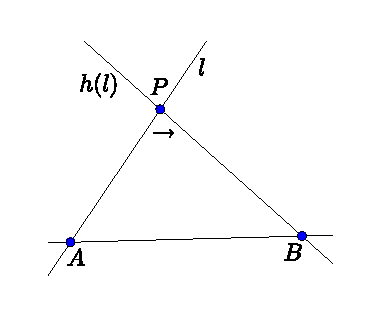
\includegraphics[scale=.8]{Graficos/Conicas/TeoremaSteiner}
	\end{center}
\end{theo}
\begin{proof}Dividamos la demostración en dos partes:
	\begin{enumerate}
		\item La homografía $h$ no es una perspetividad.
		
		Para demostrar que los puntos $P=l\cap h(l)$ se encuentran en una cónica, determinemos primero la homografía $h$. Es decir, dada una recta arbitraria del $\haz_A$, encontremos una expresión de su imagen. Para ello, dado que es una homografía, necesitamos tres puntos y sus imagenes, en este caso tres rectas y sus imágenes. A su vez, para poder describir estas rectas, necesitamos fijar una referencia proyectiva.
		
		Observemos que la recta $AB$ pertenece a ambos haces. Por tanto, tendrá tanto una imagen a través de $h$ como una imagen inversa. Esto nos permite tomar como referencia los puntos $A,B$ y $X_0=h^{-1}(AB)\cap h(AB)$, más un punto unidad $e$ que determinaremos más adelante. Podríamos preguntarnos el porqué de esta elección. Hagamos unas pequeñas observaciones y en seguida lo entenderemos.
		 \begin{center}
		 	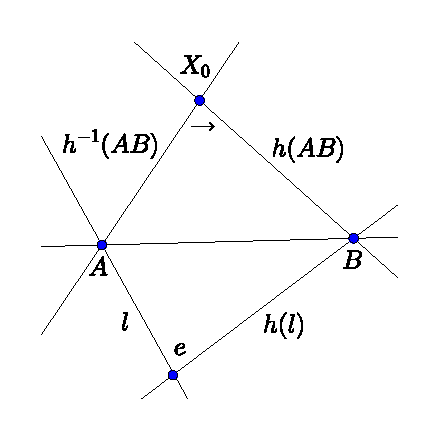
\includegraphics[scale=.8]{Graficos/Conicas/TeoremaSteiner1}
		 \end{center}
		Notemos que $h^{-1}(AB)$ es una recta que pertenece al $\haz_A$ y que pasa por $X_0$. Por tanto, no tiene más remedio que ser la recta $AX_0$. Lo mismo ocurre con la recta $h(AB)$, que pertenece al $\haz_B$. Por ello, $h(AB)=BX_0$. Esto implica que $BX_0$ es la imagen, a través de la homografía, de $AB$ y que $AB$ es la imagen de $AX_0$. 
		
		Tenemos pues dos rectas ($AB$ y $AX_0$) y sus imágnes ($BX_0$ y $AB$). Nos falta una tercera, que será una recta $l$ del $\haz_A$ distinta de $AB$. Tomemos entonces el punto unidad $e=l\cap h(l)$. De esta forma $l=Ae$ y $h(l)=Be$. Como hemos escogido la referencia \[\mf{R}=\{A,X_0,B;e\}=\{(1:0:0),(0:1:0),(0:0:1),(1:1:1)\}\]
		las ecuaciones implícitas de las rectas son
		\begin{equation*}
			AB:y=0, \quad AX_0: z=0, \quad BX_0:x=0, \quad l:y-z=0, \quad h(l):x-y=0
		\end{equation*}
		de tal forma que la homografía
		\begin{equation*}
			\begin{array}{cccc}
			h:&\haz_A&\rightarrow&\haz_B\\
			&z=0 &\rightarrow& y=0\\
			&y=0 &\rightarrow& x=0\\
			&y-z=0 &\rightarrow& x-y=0
			\end{array}
		\end{equation*}
		Con esto queda totalmente determinada la homografía $h$. Se trata de aquella homografía que trasforma la referencia $\mf{R}_A=\{z=0,y=0;y-z=0\}$ en $\mf{R}_B=\{y=0,x=0;x-y=0\}$. Equivalentemente, $\widehat{h}:\mc{B}_A\rightarrow \mc{B}_B$, donde las bases asociadas son $\mc{B}_A=\{y=0,-z=0\}$ y $\mc{B}_B=\{x=0,-y=0\}$.
		
		Para poder encontrar la expresión de la imagen de una recta arbitraria del haz con base $A$, debemos parametrizar ambos haces. Esto se puede hacer con dos cualesquiera de sus rectas. Tomemos las parametrizaciones
		\begin{equation*}
			\haz_A=\{y-\theta z=0\tq \theta\in\overline{\K}\}, \quad \haz_B=\{x-\theta y=0\tq \theta\in\overline{\K}\}
		\end{equation*}
		Por tanto, la imagen de cualquier recta arbitraria del $\haz_A$, que se puede escribir como $y-\theta z=0$, es la recta $x-\theta y=0$.
		
		Por fin podemos hallar la expresión de un punto $P=l\cap h(l)$ arbitrario. Este no será otro que la intersección de las rectas $y-\theta z=0$ y $x-\theta y=0$. Realizando este sencillo cálculo obtenemos que los puntos $P$ son los puntos $\{(\theta^2:\theta:1)\tq \theta\in\overline{\K}\}$. Dado que esta es la parametrización de una parábola, queda demostrado que engendran una cónica no degenerada. Por otro lado, la unicidad proviene del hecho de que cinco puntos, no estando cuatro de ellos alineados, determinan una única cónica.
		
		\item La homografía $h$ es una perspectividad. 
		
		Al ser una homografía, es claro que el conjunto de puntos $\{P=l\cap h(l)\tq l\in \haz_A\}$ engendran una única cónica. Debemos demostrar que esta cónica es degenerada si y solo si $h$ es una perspectividad.
		
		Si la homografía $h$ es una perspectividad, entonces $h(l)=\engen{O^*\cap l,B}$, donde $O^*$ es la recta base de la perspectividad. Además, deja fija la recta $AB$. Por tanto, $\{P=l\cap h(l)\tq l\in \haz_A\}=O^*\cup AB$, es decir, contiene una recta. Se concluye que la cónica es degenerada.
		
		Por otro lado, si la cónica engendrada por los puntos $P=l\cap h(l)$ con $l\in\haz_A$ es degenerada, entonces será producto de dos rectas. Aplicando la observación~\ref{C8_obs_conicaProducto_union} se tiene que $\{P=l\cap h(l)\tq l\in \haz_A\}=m\cup r$ para ciertas rectas $m$ y $r$. Basta demostrar que una de esas rectas es la recta $AB$. En tal caso, dado $P\in AB$ tal que $P=l\cap h(l)$ para cierta recta $l$ del haz con base $A$, se tiene que $l=PA$ y $h(l)=PB$. Como $P\in AB$, se concluye que $l=AB$ y $h(l)=AB$. Por tanto, la recta $AB$ queda fija. Esto implica que $h$ es perspectividad.
		
		Demostremos por tanto que $m$ o $r$ es la recta $AB$. Recordemos del primer apartado que $A=h^{-1}(AB)\cap AB$ y $B=AB\cap h(AB)$. Por tanto, $A$ y $B$ pertenecen a la cónica, y, con ello, $A,B\in m\cup r$. Si ambos puntos se encuentran en la misma recta, no hay nada que demostrar. Supongamos, por tanto, que $A\in m$ y $B\in r\backslash r\cap m$, lo cual implica que $m\in \haz_A$ y $r\in \haz_B$, y lleguemos a un absurdo.
		
		Sea $l\in \haz_A$ distinta de $m$. Entonces $P=l\cap h(l)\in r$, ya que en caso contrario $P\in m$ y entonces $l=PA=m$. Como $h(l)=PB$ y $P,B\in r$, se conlcuye que $h(l)=r$ para toda recta $l$ del $\haz_A$ distinta de $m$. Esto es absurdo ya que $h$ es una homografía.
		
		Con esto queda demostrado que $A,B$ deben pertenecer a la misma recta y, con ello, que $AB$ permanece fija.
	\end{enumerate}
\end{proof}
\begin{obs}
	\label{C8_homografia_Steiner_tangentes}
	Sabemos que, dada una homografía $h$ entre haces de rectas, los puntos $P=l\cap h(l)$ son una cónica. Recordemos que $A$ y $B$ pertenecían a la cónica. Por tanto, la recta $l$ corta a la cónica en los puntos $P$ y $A$. Con ello,  $h(l)$ es la recta que pasa por $B$ y $P$, siendo este último el punto de corte de $l$ con la cónica distinto de $A$. Gracias a esto podemos saber adonde manda $h$ determinadas rectas del haz. 
	
	En concreto, la tangente $l$ a la cónica en el punto $A$ se transforma en la recta $AB$. En efecto, abusando del lenguaje, podemos decir que la tangente a $A$ corta a la cónica en el punto $A$ y en el punto $A$. Dado que su imagen es la recta que pasa por $B$ y el otro punto de corte que no es $A$, $h(l)$ es la recta $AB$. De forma similar se deduce que $AB$ se transforma en la recta tangente a $B$.
\end{obs}
Veamos un ejemplo del teorema anterior.
\begin{exa}[Aplicación del Teorema de Steiner]
	Calcúlese la cónica asociada a la homografía $h$ entre haces de rectas que transforma $x=-2z$, $3x+2y=2z$, $2x+3y=8z$ en las rectas $x-2y=-2z$, $x=2z$, $x+y=4z$, respectivamente.\\
	
	Para calcular la cónica debemos hallar los puntos de la forma $P=l\cap h(l)$. Para ello, tomaremos una recta genérica del primer haz y la cortaremos con su imagen, obteniendo así una parametrización de $\{P=l\cap h(l)\tq l\in \haz\}$, y con ello de la cónica.
	
	Es necesario que primero parametricemos los haces de rectas. Las rectas dadas se corresponden con los siguientes puntos del dual:
	\begin{equation*}
		\begin{split}
			a_0=(1:0:2), \quad a_1=(3:2:-2), \quad a_2=(2:3:-8)\\
			b_0=(1:-2:2), \quad b_1=(1:0:-2), \quad b_2=(1:1:-4)
		\end{split}
	\end{equation*}
	de tal forma que la homografía $h$ transforma $a_i$ en $b_i$. Tomamos como referencia del primer haz $\mf{R}=\{a_0,a_1;a_2\}$ y, como referencia del segundo, $\overline{\mf{R}}=\{b_0,b_1;b_2\}$, de tal forma que $h:\mf{R}\rightarrow  \overline{\mf{R}}$. Realizando unas sencillas cuentas obtenemos que las bases asociadas son $\mc{B}=\{(-5,0,-10),(9,6,-6)\}$ y $\overline{\mc{B}}=\{(-1,2,-2),(3,0,-6)\}$. Así, $\widehat{h}$ transforma $\mc{B}$ en $\overline{\mc{B}}$.
	
	De esta forma, una recta genérica del primer haz $l=\class{(9\theta-5,6\theta,-6\theta-10)}$ se transforma en $h(l)=\class{(3\theta-1,2, -6\theta-2)}$.
	
	La parametrización de la cónica, los puntos $P=l\cap h(l)$, viene dada por la intersección de estas dos rectas. Este es un cálculo común, cuyo resultado es
	\begin{equation*}
		\mc{C}=\{(18\theta^2-10,-18\theta^2+18\theta,9\theta^2-12\theta+5)\tq \theta\in\overline{\K}\}
	\end{equation*}
	Podríamos hallar la matriz asociada a esta cónica. Para ello, dada una matriz genérica
	\begin{equation*}
		A=\left( \begin{array}{ccc}
			a & h & g\\
			h & b & f\\
			g & f & c
		\end{array}\right) 
	\end{equation*}
	debemos resolver la ecuación
	\begin{equation*}
		X^tAX=0
	\end{equation*}
	donde $X=(18\theta^2-10,-18\theta^2+18\theta,9\theta^2-12\theta+5)$. Esto nos dará un polinomio de segundo grado cuyos coeficientes deben ser todos nulos, para que se cumpla la ecuación de la cónica. Resolviendo las ecuaciones resultantes de igualar cada uno de los coeficientes a cero, obtenemos que
	\begin{equation*}
		a=1, \ b=2, \ c=-8, \ h=1, \ f=-2, \ g=-1
	\end{equation*}
	Por tanto, la matriz de la cónica es
	\begin{equation*}
		A=\left( \begin{array}{ccc}
			1 & 1 & -1\\
			1 & 2 & -2\\
			-1 & -2 & -8
		\end{array}\right) 
	\end{equation*}
	siendo por tanto su ecuación
	\begin{equation*}
		\mc{C}=x^2+2y^2-8z^2+2xy-2xz-4yz=0.
	\end{equation*}
\end{exa}

\section{Razón doble en cónicas}
Como ya anticipamos, dado que toda cónica es un $\proy^1$, podemos definir en ellas la razón doble. Antes, y para asegurarnos de que la definición sea buena, enunciaremos un teorema.

\begin{theo}[Teorema de Chasles]
	Sea una cónica $\mc{C}$ no degenerada y dos puntos $P,P'\in\mc{C}$. Entonces, la aplicación entre haces de rectas definida como
	\begin{equation}\label{C8_eq_teo_chasles}
		\begin{array}{cccc}
		h:& \haz_P&\rightarrow &\haz_{P'}\\
		& l&\rightarrow & h(l)=P'Q
		\end{array}
	\end{equation}
	donde $l\cap\mc{C}=\{P,Q\}$, es una homografía.
\end{theo}
\begin{proof}
	Tomamos la referencia $\mf{R}=\{P,X_1,P';e\}$, de tal forma que $e\in\mc{C}$ sea distinto a $P$ y $P'$ y que $X_1$ sea el polo de $PP'$. Por la sección~\ref{C8_subsec_parametrizacion_como_parabola} sabemos que, en este referencia, la cónica se parametriza como
	\begin{equation*}
		\mc{C}=\{(\theta^2:\theta:1)\tq\theta\in\overline{\K}\}
	\end{equation*}
	Podemos describir una recta arbitraria de $\haz_P$ como $l=PQ$, siendo $l\cap\mc{C}=\{P,Q\}$, es decir, tomamos Dado que $Q$ es un punto de la cónica, tendrá coordenadas $(\theta^2:\theta:1)$. Además, por la referencia elegida, $P=(1:0:0)$. Con ello, $l:y-\theta z=0$. De la misma forma, su imagen ($h(l)=P'Q$) será la recta $x-\theta y=0$.
	
	Por tanto, la aplicación proyectiva $h$ transforma $y-\theta z=0$ en $x-\theta y=0$. Pasando a coordenadas no homogéneas, $h:\theta\rightarrow \theta$, por lo que es la identidad y, por tanto, es homografía.
\end{proof}
\begin{obs}
	Obsérvese que este teorema es el recíproco del Teorema de Steiner y nos liga dos haces cualesquiera con base un punto de la cónica. Para hallar las imágenes de ciertas rectas podemos tener en cuenta la observación~\ref{C8_homografia_Steiner_tangentes}.
\end{obs}
\begin{defi}\label{C8_def_razondoble}
	Dada una cónica $\mc{C}$, se define la razón doble de cuatro puntos $P_1,P_2,P_3,P_4\in\mc{C}$ como
	\begin{equation}
		\{P_1,P_2;P_3,P_4\}=\{PP_1,PP_2;PP_3,PP_4\}
	\end{equation}
	donde $P\in\mc{C}$ es un punto arbitrario distinto de los otros cuatro.
\end{defi}
Comprobemos que está bien definida, es decir, que no depende del quinto punto $P\in\mc{C}$ que elijamos. Sea entonces otro punto distinto $P'\in\mc{C}$ y tomemos los haces $\haz_P$ y $\haz_P'$. Por el Teorema de Chasles sabemos que, la aplicación proyectiva $h$ entre los haces definida por la ecuación~\eqref{C8_eq_teo_chasles}, es una homografía. Además, por la observación~\ref{C8_obs_conica_recta_interseccion2puntos} sabemos que una recta corta en dos puntos a una cónica. Dado que $P,P_i\in\mc{C}$, para $i=1,2,3,4$, se tiene que la recta $PP_i$ corta con $\mc{C}$ en los puntos $P$ y $P_i$. Por tanto, como las homografías preservan la razón doble,
\begin{equation}
	\{PP_1,PP_2;PP_3,PP_4\}=\{h(PP_1),h(PP_2);h(PP_3),h(PP_4)\}=\{P'P_1,P'P_2;P'P_3,P'P_4\}
\end{equation}
quedando así demostrado que la razón doble está bien definida.

\subsection{Cálculo de la razón doble}
Hemos definido la razón doble de cuatro puntos de una cónica como la razón doble de cuatro rectas. Por tanto, el cálculo es el mismo que cuando veíamos este caso en el capítulo Razón Doble.\\

Obsérvese que si paramétrizamos la cónica con la referencia adecuada, los puntos $P_i$ pueden escribirse como $P_i=(\theta_i^2:\theta_i:1)$. Si tomamos como quinto punto el $X_0=(1:0:0)\in\mc{C}$ de la referencia entonces, las rectas de la definición de razón doble son $X_0P_i:y-\theta_iz=0$. En el espacio proyectivo dual serían $X_0P_i=(0:1:-\theta_i)$. 

Siguiendo lo visto en el capítulo cinco, la razón doble de $P_1,P_2,P_3,P_4\in\mc{C}$ es
\begin{multline}
	\{P_1,P_2;P_3,P_4\}=\{PP_1,PP_2;PP_3,PP_4\}=\\=\{(0:1:-\theta_1),(0:1:-\theta_2);(0:1:-\theta_3),(0:1:-\theta_4)\}=\{\theta_1,\theta_2;\theta_3,\theta_4\}
\end{multline}\\
De forma más general, si la cónica está parametrizada por tres polinomios, de tal forma que $P_i=(p_0(\theta_i),p_1(\theta_i),p_1(\theta_i))$, la razón doble es
\begin{equation}
\{P_1,P_2;P_3,P_4\}=\{\theta_1,\theta_2;\theta_3,\theta_4\}
\end{equation}
En efecto, basta tener en cuenta el cambio de coordenadas $\rho\overline{X}=HX$, donde $H$ viene dada por 
\begin{equation*}
	\left( \begin{array}{c}
	p_1(\theta)\\p_2(\theta)\\p_3(\theta)
	\end{array}\right)=H
	\left( \begin{array}{c}
	\theta^2\\\theta\\1
	\end{array}\right)
\end{equation*}
que nos permite pasar de la referencia $\mf{R}$ en la cual la cónica es una parábola, a la referencia donde la cónica viene parametrizada por los polinomios dados. Aunque el punto $P_i=(x_i:y_i:z_i)$ puede tener diferentes coordenadas en la referencia $\mf{R}$, el valor de $\theta$ será el mismo. Teniendo en cuenta esto y el resultado anterior, se tiene que
\begin{equation*}
	\{P_1,P_2;P_3,P_4\}=\{\theta_1,\theta_2;\theta_3,\theta_4\}
\end{equation*}

\subsection{Razón doble en cónicas duales}
Por supuesto, todo esto tiene su análogo dual. Primero veamos que tenemos derecho a definir el concepto de razón doble en una cónica dual. Como vimos, toda cónica es un $\proy^1$. Dado que la dimensión de un espacio proyectivo y su dual coinciden, toda cónica dual es un $\proy^1$. Por tanto, podemos definir razón doble. De hecho, esta definición no será más que el dualizado de la definición anterior.
\begin{defi}
	Dada una cónica dual $\mc{C}^*$, se define la razón doble de cuatro rectas $l_1,l_2,l_3,l_4\in\mc{C}^*$ como
	\begin{equation}
		\{l_1,l_2;l_3,l_4\}=\{l\cap l_1,l\cap l_2;l\cap l_3,l\cap l_4\}
	\end{equation}
	donde $l\in\mc{C}^*$ es una recta arbitraria distinta de las otras cuatro.
\end{defi}
Es claro que esta definición es buena, es decir, que no depende de $l$, ya que es simplemente el dualizado de la definición~\ref{C8_def_razondoble} (la cual no dependía de $P$).

Es lógico pensar que la razón doble de cuatro rectas de la cónica dual, que son rectas tangentes a $\mc{C}$ en un punto, sea igual que la razón doble de los puntos de tangencia. Recordemos que estos puntos de tangencia eran los polos de las rectas tangentes. Por tanto, nos gustaría que, si $P_i=A^*l_i$, entonces $\{l_1,l_2;l_3,l_4\}=\{P_1,P_2;P_3,P_4\}$, donde $A^*$ es la adjunta de la matriz de la cónica. Para llegar a este resultado necesitamos un lema previo.
\begin{lem}
	Sea una cónica $\mc{C}$ y un punto $P$. La aplicación
	\begin{equation}
		\begin{array}{cccc}
		g:&\haz_P&\rightarrow &\proy^2\\
		&l&\rightarrow & Q
		\end{array}
	\end{equation}
	donde $Q$ es el polo de $l$, es una homografía cuya imagen es la recta polar de $P$.
\end{lem}
\begin{proof}
	Tomemos $l_1$ y $l_2$ dos rectas del haz para hallar su ecuación paramétrica. Así
	\begin{equation*}
		\haz_P=\{l=l_1+\theta l_2\tq\theta\in\overline{\K}\}
	\end{equation*}
	Si $C$ es la matriz asociada a la cónica, el polo de una recta $l$ genérica viene dado por
	\begin{equation*}
		Q=A^*l=A^*(l_1+\theta l_2)=A^*l_1+\theta A^*l_2
	\end{equation*}
	De esta forma, la aplicación definida en el enunciado puede describirse de la siguiente forma
	\begin{equation*}
		\begin{array}{cccc}
		g:&\haz_P&\rightarrow &\proy^2\\
		&l_1+\theta l_2&\rightarrow & A^*l_1+\theta A^*l_2
		\end{array}
	\end{equation*}
	La imagen de $g$ recorre la recta $A^*l_1+\theta A^*l_2$. Además, en coordenadas no homogéneas, $g:\theta\rightarrow \theta$, por lo que es una homografía.
	
	Veamos que esta recta es la Polar($P$). Dado que $Q$ es el polo de $l$, la recta $l$ es la recta Polar($Q$). Como $P\in l$ para cualquier recta del haz, se tiene que $P\in$ Polar($Q$) y, por tanto, $Q$ está en Polar($P$). Con esto se tiene que los polos de las rectas del haz pertenecen a la recta polar de $P$. Como también pertenecen a la recta $A^*l_1+\theta A^*l_2$ se concluye que esta es la polar de $P$.
\end{proof}
Con esto ya podemos realizar la demostración cómodamente.
\begin{prop}
		Dada una cónica dual $\mc{C}^*$ y cuatro rectas $l_1,l_2,l_3,l_4\in\mc{C}^*$ y sus respectivos puntos de tangencia $P_1,P_2,P_3,P_4\in\mc{C}$, se tiene que 
		\begin{equation}
		\{l_1,l_2;l_3,l_4\}=\{P_1,P_2;P_3,P_4\}
		\end{equation}
\end{prop}
\begin{proof}
	Basta probar que la aplicación proyectiva definida por
	\begin{equation*}
		\begin{array}{cccc}
			h:&\mc{C}&\rightarrow &\mc{C}^*\\
			& P&\rightarrow &l=Polar(P)
		\end{array}
	\end{equation*}
	es una homografía. En efecto, en tal caso, dado que la recta polar de un punto perteneciente a la cónica es la recta tangente en ese punto, el resultado se sigue.
	
	Vayamos con la comprobación. Sea un punto $V\in\mc{C}$ distinto de $P$ consideremos la siguiente composición de homografías
	\begin{equation*}
		\begin{array}{ccccccc}
			\mc{C}&\xrightarrow{h_1}&\haz_V&\xrightarrow{g}& Polar(V)&\xrightarrow{h_2}&\mc{C}^*\\
			P&\rightarrow &PV&\rightarrow&Q&\rightarrow&QP
		\end{array}
	\end{equation*}
	donde $g$ es la homografía del lema anterior, por lo que $Q$ es el polo de $PV$.
	
	Tomemos la composición $h_2\circ g\circ h_1$ y veamos que está bien definida. La recta $PV$ es la recta polar de $Q$. Como sabemos, las rectas engendradas por $Q$ y los puntos de corte de Polar($Q$) con la cónica, son rectas tangentes a la misma. Como $P$ es uno de estos puntos, la recta $QP$ es tangente y, por tanto, pertenece a la cónica dual. Además, por ser tangente en el punto $P$ se trata de la recta polar de $P$. Esto implica que $h=h_2\circ g\circ h_1$. Como la composición de homografías es homografía, hemos terminado.
	\begin{center}
		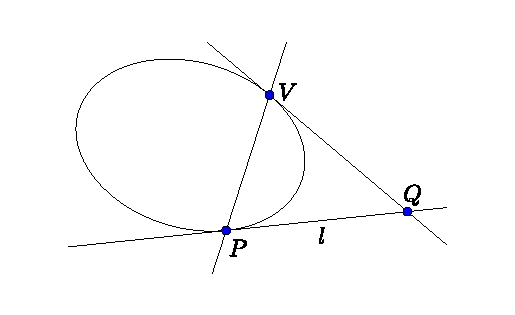
\includegraphics[scale=.8]{Graficos/Conicas/RazonDobleDual}
	\end{center}
\end{proof}
\begin{obs}
	No se ha obviado el hecho de que en la demostración anterior no se ha comprobado que las aplicaciones $h_1$ y $h_2$ son homografías. Dado que la demostración sirven para afianzar conceptos, se deja como ejercicio al lector.
\end{obs}

\section{Involuciones de la cónica}

Dado que toda cónica es un $\proy^1$, se pueden definir involuciones en la cónica. En esta sección se demostrará un resultado realmente fuerte, ya que nos proporciona una forma de construir cualquier involución de la cónica.

\begin{prop}
	Dada una cónica $\mc{C}$ no degenerada y un punto $X_1\not\in\mc{C}$, el conjunto de pares $(P,P')$ de puntos de $\mc{C}$ alineados con $X_1$ definen una involución de la cónica. Además, todas las involuciones de $\mc{C}$ se construyen de este modo.
	\begin{center}
		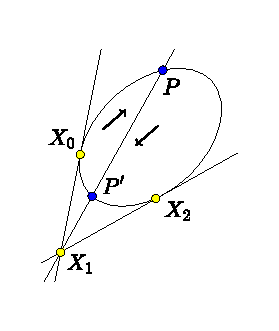
\includegraphics[scale=1]{Graficos/Conicas/Involucion}
	\end{center}
\end{prop}
\begin{proof}
	Sean $X_0$ y $X_2$ los puntos de corte de las rectas tangentes desde $X_1$ a $\mc{C}$ y $e\in\mc{C}$ otro punto distinto. Tomemos la referencia $\mf{R}=\{X_0,X_1,X_2;e\}$, que sabemos que nos parametriza la cónica como una parábola. Así, el par de puntos $(P,P')$ alineados con $X_1$ pueden escribirse como $P=(\theta^2:\theta:1)$ y $P'=(\theta'^2:\theta':1)$.
	
	El hecho de que la aplicación definida por el conjunto de pares $(P,P')$ sea involutiva es obvio. Nos queda pues probar que es una homografía distinta de la identidad para demostrar que es una involución. Para ello, basta encontrar una relación  entre $\theta$ y $\theta'$ que sea una homografía.
	
	La recta $PP'$ viene dada por
	\[\left| \begin{array}{ccc}
		x&y&z\\
		\theta^2&\theta&1\\
		\theta'^2&\theta'&1
	\end{array}\right| =0\]
	Además, $X_1=(0:1:0)$ perteneces a la recta $PP'$ si y solo si
	\[\left| \begin{array}{ccc}
	0&1&0\\
	\theta^2&\theta&1\\
	\theta'^2&\theta'&1
	\end{array}\right| =0\sii \theta^2-\theta'^2=0\sii \theta=\pm\theta'\]
	La relación no puede ser $\theta=\theta'$ ya que en ese caso la recta que pasa por $X_1$ cortaría a la cónica en un solo punto doble, y eso solo ocurre con las dos rectas tangentes. Por tanto, $\theta=-\theta'$, relación que define una homografía distinta de la identidad entre los puntos $(P,P')$. De hecho, es una relación involutiva, pues el módulo $k=-1$. Queda demostrado pues que se trata de una involución.\\
	
	Veamos que toda involución de la cónica se construye de este modo.
	
	Sea $h$ una involución de la cónica, definida por la ecuación general
	\begin{equation*}
		\alpha\theta'\theta+\beta(\theta'+\theta)+\delta=0
	\end{equation*}
	Tomamos entonces el punto $X_1=(\delta:-\beta:\alpha)$. Demostremos que la involución definida a partir de este punto es la misma que la original. Para ello, de nuevo, hallemos la relación entre las coordenadas no homogéneas de dos puntos $P=(\theta^2:\theta:1)$ y $P'=(\theta'^2:\theta':1)$ alineados con $X_1$. Como acabamos de ver, esta viene dada por
	\[\left| \begin{array}{ccc}
	\delta&-\beta&\alpha\\
	\theta^2&\theta&1\\
	\theta'^2&\theta'&1
	\end{array}\right| =0\sii \delta(\theta-\theta')+\beta(\theta^2-\theta'^2)+\alpha(\theta^2\theta'-\theta'^2\theta)=0\]
	Como $P\not=P'$, se tiene que $(\theta-\theta')\not=0$, pudiendo así dividir por ello. Queda
	\[\delta +\beta(\theta+\theta')+\alpha\theta\theta'=0\]
	que es precisamente la ecuación de la involución original.
\end{proof}
\begin{obs}
	Otra forma de demostrar el ``\ti{además}'' de la proposición es considerar una involución de la cónica y dos pares de la misma. Esos dos pares determinan dos rectas que se cortan en un punto. Al considerar la involución a partir de ese punto de corte (con la construcción de la proposición) esta coincidirá con la original en los dos pares elegidos. Como una involución queda determinada por dos pares, son la misma involución.
\end{obs}
\begin{obs}
	Observemos que los dos puntos fijos de una involución construida a partir de un punto $X_1$ son los puntos de corte de la recta Polar($X_1$) con la cónica.
\end{obs}

\section{Homografías de la cónica}
Al igual que con las involuciones, se pueden definir en la cónica todo tipo de homografías. Por ello, conviene recuperar algunos de los teoremas más importantes relacionados con las homografías y dar a conocer otros nuevos.

\begin{theo}[Teorema del Eje]
	Sea $\mc{C}$ una cónica no degenerada y $h:\mc{C}\rightarrow\mc{C}$ una homografía. Entonces el conjunto
	\begin{equation}
		\{Ph(Q)\cap h(P)Q\tq PQ\in\mc{C}\}
	\end{equation}
	es una recta, denominada \ti{eje de la homografía}.
\end{theo}
\begin{proof}
	Para realizar la demostración de este teorema dividamos las homografías en dos grupos, aquellas con dos puntos fijos distintos y las homografías con un punto fijo doble. Dado que nos encontramos en $\C$ es seguro que esto engloba todas las posibles homografías.\\
	
	\underline{Caso 1}: Sea $h$ una homografía con dos puntos fijos distintos $M$ y $N$. Tomemos como referencia $\mf{R}=\{M,X_1,N,e\}$ donde $X_1$ es el polo de la recta $MN$ y $e$ es un punto de la cónica distinto a los demás. De esta forma, la cónica queda parametrizada como una parábola. Además, los puntos fijos pasan a ser el cero y el infinito. Recordemos del tema $6$ que en tal caso la ecuación de $h$ es 
	\[\theta'=k\theta\]
	donde $k$ es el módulo de la homografía.
	
	Por tanto, si 
	\[P=(\theta_0^2:\theta_0:1),\quad Q=(\theta_1^2:\theta_1:1)\]
	sus imágenes son
	\[h(P)=(k^2\theta_0^2:k\theta_0:1),\quad h(Q)=(k^2\theta_1^2:k\theta_1:1)\]
	Para hallar los puntos $Ph(Q)\cap h(P)Q$, escribamos las ecuaciones de las rectas $Ph(Q)$ y $h(P)Q$ y solucionemos el sistema. De forma general, la recta que pasa por dos puntos distintos de la cónica $(\theta^2:\theta:1)$ y $(\theta'^2:\theta':1)$ viene dada por 
	\[\left| \begin{array}{ccc}
	x&y&z\\
	\theta^2&\theta&1\\
	\theta'^2&\theta'&1
	\end{array}\right| =0\sii x(\theta-\theta')-y(\theta^2-\theta'^2)+z(\theta^2\theta'-\theta'^2\theta)=0\]
	Como son puntos distintos, y como ya hicimos antes, podemos dividir por $(\theta-\theta')$, y queda
	\begin{equation}\label{C8_eq_teo_eje}
		x -y(\theta+\theta')+z\theta\theta'=0
	\end{equation}
	Particularicemos al caso que nos atañe. El sistema de ecuaciones a resolver es:
	\begin{equation*}
		\begin{split}
			Ph(Q):& \ x-(\theta_0+k\theta_1)y+k\theta_0\theta_1z=0\\
			Qh(P):& \ x-(\theta_1+k\theta_0)y+k\theta_1\theta_0z=0
		\end{split}
	\end{equation*}
	Restando ambas ecuaciones obtenemos
	\[(1-k)(\theta_1-\theta_0)y=0\]
	Como no se trata de identidad $k\not=1$. Además, $\theta_0\not=\theta_1$. Por tanto, podemos reducir la ecuación anterior a
	\[y=0\]
	Es decir, cualquier solución del sistema de ecuaciones, que son los puntos $Ph(Q)\cap h(P)Q$ que pertenecen a ambas rectas, está en la recta $y=0$. Obsérvese que con esto no solo hemos demostrado que el conjunto
	\[\{Ph(Q)\cap h(P)Q\tq PQ\in\mc{C}\}\]
	es una recta, sino que esa recta, el eje de la homografía, es \tb{la recta que pasa por los puntos fijos}.\\
	
	\underline{Caso 2}: Sea $h$ una homografía con un punto fijo doble $M$. Consideremos puntos $X_2\in\mc{C}$ y $X_1\not\in\mc{C}$ tales que $X_1$ sea el polo de la recta $MX_2$. Tomemos entonces la referencia $\mf{R}=\{M,X_1,X_2;e\}$, donde $e$ es un punto distinto de la cónica. De nuevo, en esta referencia, la cónica se parametriza como una parábola. Además, el punto fijo pasa a ser el infinito. Por lo visto en el tema $6$, la ecuación de la homografía en esta referencia es
	\[\theta'=\theta+\mu\]
	Al igual que ante, para hallar los puntos $Ph(Q)\cap h(P)Q$, escribiremos las ecuaciones de las rectas $Ph(Q)$ y $h(P)Q$ y solucionaremos el sistema. Aprovechándonos de la ecuación~\ref{C8_eq_teo_eje} el sistema a resolver es
	\begin{equation*}
		\begin{split}
			Ph(Q):& \ x-(\theta_0+\theta_1+\mu)y+\theta_0(\theta_1+\mu)z=0\\
			Qh(P):& \ x-(\theta_1+\theta_0+\mu)y+\theta_1(\theta_0+\mu)z=0
		\end{split}
	\end{equation*}
	Restando ambas ecuaciones obtenemos
	\[\mu(\theta_0-\theta_1)z=0\]
	Dado que la homografía no es la identidad, $\mu\not=0$. Como los puntos elegidos son distintos se tiene que cualquier solución del sistema de ecuaciones, es decir, los puntos $Ph(Q)\cap h(P)Q$, están en la recta $z=0$. De nuevo, no solo hemos demostrado lo pedido, sino que además hemos probado que en el caso de que la homografía tenga un punto fijo doble, el eje de la homografía es \tb{la recta tangente a la cónica en el punto fijo}.
\end{proof}
\begin{obs}\label{C8_obs_determinaciom_homconica_eje}
	Dada una homografía $h:\mc{C}\rightarrow\mc{C}$, la imagen por $h$ de cualquier punto $X\in\mc{C}$ puede construirse usando los puntos fijos de la homografía. En efecto, si conocemos otro punto $P$, su imagen $h(P)$ y los puntos fijos (o el punto fijo), como estos me determinan el eje de la homografía y sabemos que $Ph(X)\cap h(P)X$ está en el eje, conocemos $XP'\cap eje$. Con lo cual, podemos hallar $h(X)$. Esto se muestra en las siguientes figuras.
	\begin{center}
		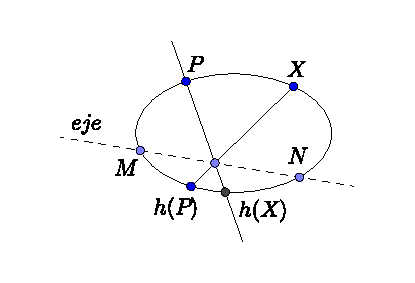
\includegraphics[scale=1]{Graficos/Conicas/TeoremaDelEje1} \
		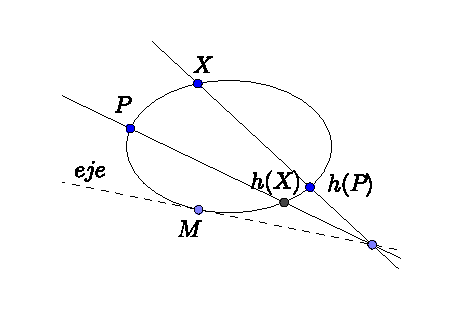
\includegraphics[scale=.9]{Graficos/Conicas/TeoremaDelEje2}
	\end{center}
\end{obs}

Para terminar esta sección, demostremos un teorema que relaciona cónicas y hexágonos.

\begin{theo}[Teorema de Pascal]
	Hay una cónica no degenerada que pasa por los puntos de un hexágono si y solo si los puntos de intersección de los lados opuestos del hexágono son colineales. Esto es si y solo si los puntos
	\begin{equation}
		A_1A_2\cap A_5A_4, \quad A_1A_6\cap A_3A_4, \quad A_5A_6\cap A_3A_2
	\end{equation}
	son colineales, donde los puntos $A_1,A_2,A_3,A_4,A_5,A_6$ se muestran en la figura.
	\begin{center}
		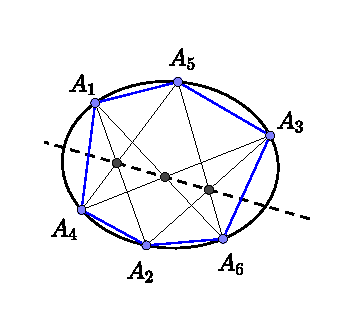
\includegraphics[scale=1]{Graficos/Conicas/TeoremaPascal}
	\end{center}
\end{theo}
\begin{proof}
	$\bra$ Supongamos que los seis puntos de un hexágono $A_1,A_2,A_3,A_4,A_5,A_6$ pertenecen la cónica no degenerada $\mc{C}$. Por lo visto en el capítulo de homografías, y dado que la cónica es un $\proy^1$, existe una única homografía de la cónica $h$ que transforma
	\begin{equation*}
		\begin{array}{cccc}
			h:&\mc{C}&\rightarrow &\mc{C}\\
			& A_1&\rightarrow &A_4\\
			& A_5&\rightarrow &A_2\\
			& A_3&\rightarrow &A_6
		\end{array}
	\end{equation*}
	Por el Teorema del Eje, las intersecciones
	\begin{equation*}
		A_1A_2\cap A_5A_4, \quad A_1A_6\cap A_3A_4, \quad A_5A_6\cap A_3A_2
	\end{equation*}
	están alineadas.\\
	
	$\bla$ Sean los seis puntos de un hexágono $A_1,A_2,A_3,A_4,A_5,A_6$ supongamos que los puntos dado por
	\begin{equation*}
		A_1A_2\cap A_5A_4, \quad A_1A_6\cap A_3A_4, \quad A_5A_6\cap A_3A_2
	\end{equation*}
	están alineados. Sea $\mc{C}$ la única cónica que pasa por los cinco puntos $A_1,A_2,A_3,A_4,A_5$. Si $A_6\in\mc{C}$ ya está hecho. Supongamos, por tanto, que no es así. Entonces, el punto $A_6'=A_1A_6\cap\mc{C}$ pertenece a la cónica. Veamos que $A_6=A_6'$, concluyendo así que $A_6\in\mc{C}$.
	
	Tenemos así seis puntos de un hexágono $A_1,A_2,A_3,A_4,A_5,A_6'$ que pertenecen a una cónica. Aplicamos la implicación que acabamos de demostrar y obtenemos que los puntos
	\begin{equation*}
		A_1A_2\cap A_5A_4, \quad A_1A_6'\cap A_3A_4, \quad A_5A_6'\cap A_3A_2
	\end{equation*}
	están alineados. Denotemos por $l$ la recta a la cual pertenecen. Dado que
	\begin{equation*}
		A_1A_6'\cap A_3A_4=A_1A_6\cap A_3A_4
	\end{equation*}
	pues $A_6'\in A_1A_6$, la recta $l$ obtenida con $A_6'$ es la misma que la recta obtenida con $A_6$, pues el punto $A_1A_2\cap A_5A_4$ es idéntico. Además, esta recta $l$ es el eje de la homografía definida en el apartado anterior. Como se vio en la observación~\ref{C8_obs_determinaciom_homconica_eje}, conocidos $A_5,A_3,h(A_5)=A_2$ y el eje de la homografía, podemos hallar $h(A_3)$. Si denotamos $N=A_3A_2\cap l$, se tiene que $h(A_3)=A_5N\cap \mc{C}=A_6'$. Pero por el apartado anterior, $h(A_3)=A_6$. Se concluye pues que $A_6=A_6'$.
\end{proof}

Recordemos que una vez demostrado un teorema, por el principio de dualidad, el enunciado dual del mismo quedará demostrado. En este caso, el Teorema de Pascal Dual tiene nombre propio y se enuncia a continuación.

\begin{theo}[Teorema de Brianchon]
	Los seis lados de un hexágono son tangentes a una cónica si y solo si las rectas que unen pares de puntos opuestos del hexágono son concurrentes.
	\begin{center}
		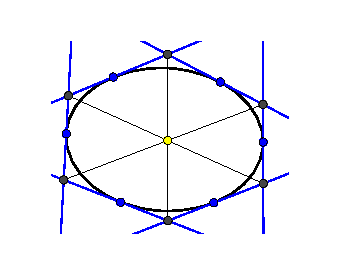
\includegraphics[scale=1.1]{Graficos/Conicas/TeoremaBrianchon}
	\end{center}
\end{theo}

\section{Clasificación de haces de cónicas}
TERMINAR. SOLO RESUMEN. NO EXPLICADO

En esta sección presentaremos las distintas situaciones que se pueden dar en los haces de cónicas, así como las situaciones duales. Un haz de cónicas queda determinado por cuatro puntos. Atendiendo a la multiplicidad con que corten las cónicas a esos puntos podemos realizar una clasificación de los haces.

Recordemos que los haces se decribían a través de
\[\mc{C}_1+\theta\mc{C}_2\]
donde $\mc{C}_1$ y $\mc{C}_2$ son dos cónicas pertenecientes al haz. Como siempre es posible encontrar una cónica no degenerada, en general, describiremos los haces como
\[S+\theta S'\]
donde $S$ es una cónica no degenerada y $S'$ es otra cónica del haz, que puede ser degenerada o no.

La clasificación es la siguiente, donde los $'$ en los número indican que nos estamos refiriendo a la situación dual.

\tb{1. Haz genérico}\\

\tb{1'. Haz dual genérico}\\

\tb{2. Haz con un punto doble}\\

\tb{2'. Haz dual con una recta doble}\\

\tb{3. Haz con un punto triple}\\

\tb{3'. Haz dual con una recta triple}\\

\tb{4. Haz con un punto cuádruple}\\

\tb{4'. Haz dual con una recta cuádruple}\\

\tb{5. Haz con dos puntos dobles}\\

\tb{5. Haz dual con dos rectas dobles}\\

Es importante observar que no siempre se puede describir un haz a partir de dos cónicas degeneradas. También resaltaremos que las situaciones duales presentadas no tienen por que ser el dual del haz. De hecho, solo hay dos situaciones autoduales (5).

Veamos un ejemplo para concluir con la clasificación.
\begin{exa}
	Dar todas las cónicas tangentes al eje de abcisas en el cero y que pasan por el $(0,1)$ y el $(1,1)$.
	\begin{center}
		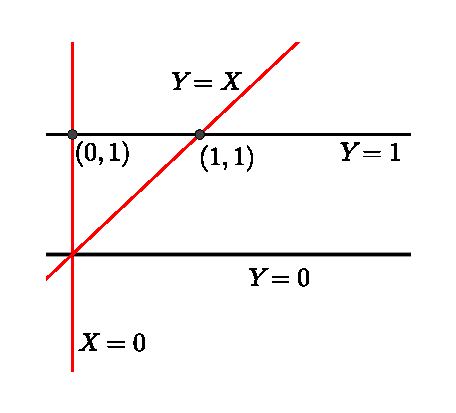
\includegraphics[scale=.8]{Graficos/Conicas/EjemploHaz}
	\end{center}
	Todas las cónicas pedidas son las cónicas de un haz con punto doble. Busquemos dos cónicas sencillas del haz para describirlo. Las más sencillas son:
	\[S:X(X-Y)=0, \quad S':Y(Y-1)\]
	Las cónicas pedidas son
	\[X(X-Y)+\theta(Y-1)Y=0\]
\end{exa}

También relacionado con los haces de cónicas, enunciemos y demostremos el siguiente teorema

\begin{theo}
	Un haz de cónicas $S+\theta S'$ genera una involución sobre cualquier recta $l$ que no pase por ninguno de los puntos de la base del haz.
	\begin{center}
		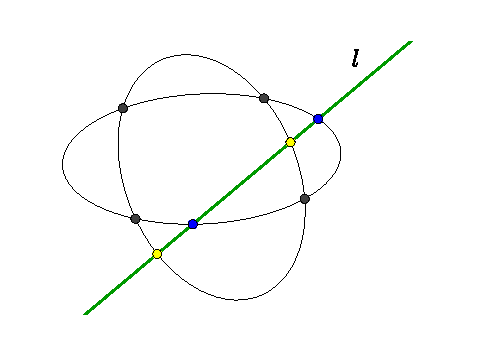
\includegraphics[scale=.9]{Graficos/Conicas/TeoremaDesargues}
	\end{center}
\end{theo}
\begin{proof}
	Sean dos puntos $P=\class{\vec{p}}$ y $Q=\class{\vec{q}}$ pertenecientes la recta $l$, podemos parametrizar esta recta como
	\[l:\{\class{\vec{p}+\theta\vec{q}}\tq\theta\in\overline{\K}\}\]
	Calculamos la intersección de la recta con el haz. Esta viene dada por la ecuación de Joachimstal
	\begin{equation*}
		(\vec{P}+\theta \vec{Q})^t(A+\theta A')(\vec{P}+\theta \vec{Q})=(\vec{P}+\theta \vec{Q})^tA(\vec{P}+\theta \vec{Q})+\theta(\vec{P}+\theta \vec{Q})^tA'(\vec{P}+\theta \vec{Q})=0
	\end{equation*}
	Cada sumando de la ecuación anterior es un polinomio de segundo grado. Por tanto, se trata de un haz de ecuaciones de segundo grado, que como vimos determina una involución. Además, nos indica que los pares de punto $(P,P')$ de la involución que el haz genera sobre $l$ son los puntos de corte de la recta $l$ con las cónicas del haz.
\end{proof}
\begin{cor}
	En general hay dos cónicas de un haz tangentes a una recta dada
\end{cor}
\begin{proof}
	Sea un haz de cónicas y una recta $l$ que no pase por ningún punto de la base del haz. Por el teorema anterior este genera una involución sobre $l$. Las involuciones tienen dos puntos fijos. Por tanto, hay dos cónicas del haz que cortan a la recta $l$ es un punto doble, es decir, que son tangentes a la misma.
\end{proof}
\begin{cor}
	Una recta genérica corta a los tres pares de lados de un cuadrilátero en pares de puntos de involución.
	\begin{center}
		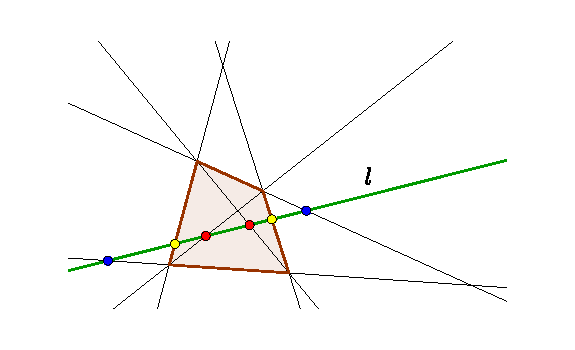
\includegraphics[scale=1]{Graficos/Conicas/CorolarioDesargues}
	\end{center}
\end{cor}
\begin{proof}
	Es una consecuencia inmediata del Teorema de Desargues ya que los tres pares de lados del cuadrilátero son tres cónicas degeneradas del haz cuyos puntos de la base son los vértices del cuadrilátero.
\end{proof}

	\chapter{Geometría Afín y Euclídea}
\label{afin}
En este capítulo repasaremos las más que probablemente olvidadas nociones de espacio afín y espacio euclídeo.

Sin embargo, lo interesante de este capítulo es que veremos cómo construir ambas estructuras a partir del espacio proyectivo. De esta forma cerraremos nuestro particular círculo virtuoso.

Además, usaremos toda esta artillería para estudiar (aun más) la geometría de las cónicas.
\section{Espacio Afín Clásico}
\label{afinClas}
En esta sección expondremos las construcciones clásicas del espacio afín que suelen verse al término de cursos de álgebra lineal elemental.
\subsection{Definición y Ejemplos}
\label{afinClasDef}
A continuación presentamos un par de posibles aproximaciones a la idea de espacio afín para, al final, demostrar su equivalencia. Haremos especial hincapié en, de alguna manera, justificar intuitivamente el por qué de ambas aproximaciones.
\subsubsection{Idea Intuitiva}
\label{afinClasDefIdea}

Recordemos como se definía un espacio afín.
\begin{defi}[Espacio afín]\label{C9_def_espacio_afin}
	Dado un conjunto no vacío $\afin$ y un espacio vectorial V, se define \ti{espacio afín}, sobre un cuerpo $\K$, a la terna $(\afin,V,\psi)$, donde
	\begin{equation*}
		\begin{array}{cccc}
			\psi: & \afin \times \afin & \rightarrow &V\\
			& (a,b) & \rightarrow & \overrightarrow{ab}
		\end{array}
	\end{equation*}
	tal que 
	\begin{enumerate}
		\item Para cada $a\in\afin$, la aplicación $\psi_a: b\rightarrow \overrightarrow{ab}$ es una biyección.
		
		\item Para cada terna $a,b,c\in\afin$, se tiene que $\overrightarrow{ab}+\overrightarrow{bc}=\overrightarrow{ac}$.
	\end{enumerate}
\end{defi}
Los elementos de $\afin$ se denominan puntos. Muy a menudo se denotará como espacio afín únicamente al conjunto $\afin$, cometiendo así un abuso de notación.

Por otro lado, $V$ se dice que es el espacio vectorial asociado al espacio afín. además, se define la dimensión del esapcio afín $\afin$ como la dimensión del espacio vectorial $V$.

La propiedad 1 de la definición nos dice que, si tenemos un espacio afín y fijamos un punto, entonces ese espacio afín pasa a ser un espacio vectorial con origen el punto fijado.

A continuación mostraremos un ejemplo que, a pesar de ser sencillo, nos permite introducir una notación muy útil.
\begin{exa}
	En el conjunto $\R^2$ podemos definir una estructura de espacio afín sobre el espacio vectorial $\R^2$. La aplicación sería 
	\begin{equation*}
		\begin{array}{cccc}
		\psi: & \R^2 \times \R^2 & \rightarrow &\R^2\\
		& (a,b)=(a_1,a_2,b_1,b_2) & \rightarrow & \overrightarrow{ab}=(b_1-a_1,b_2-a_2)
		\end{array}
	\end{equation*}
	donde $a=(a_1,a_2)$ y $b=(b_1,b_2)$ son dos puntos de $\R^2$.
	
	Debemos comprobar que la aplicación definida cumple las propiedades 1 y 2. Para cada punto $a=(a_1,a_2)$ la aplicación $\psi_a$ es inyectiva, ya que $(b_1-a_1,b_2-a_2)=(b'_1-a_1,b'_2-a_2)$ si y solo si $(b_1,b_2)=(b'_1,b'_2)$. Por otro lado, para cada $a=(a_1,a_2)$, dado $v=(v_1,v_2)\in V$, vector del espacio vectorial, el punto $b=(a_1+v_1,a_2+v_2)$ es el único que verifica $\psi_a(b)=\overrightarrow{ab}=v$. Esto prueba la sobrectividad de $\psi_a$.
	
	Es trivial comprobar que se cumple la segunda propiedad.
\end{exa} 
\begin{obs}
	Lo realizado en el ejemplo anterior no solo se puede extender a $\R^n$, definiendo $\overrightarrow{ab}=(x_1-y_1,\cdots,x_n-y_n)$, sino a cualquier espacio vectorial. Para ello, dados dos elementos $x,y\in V$, la aplicación $\psi$ queda definida por $\overrightarrow{xy}=x-y$. Es fácil, y se deja al lector, comprobar que cumple las propiedades 1 y 2.
\end{obs}
\begin{obs}[Notación]\label{c9_obs_notacion}
	Debido a la forma en la que se obtiene el punto $b=(a_1+v_1,a_2+v_2)$ en el ejercicio anterior, comúnmente se adopta la notación $b=a+v$ y se denomina el trasladado por $v$ del punto $a$. Nótese que, dados $a$ y $v$, el punto $b$ es único. además, se comete un abuso de notación, ya que el signo $+$ no representa ninguna operación.
\end{obs}

A continuación mostraremos algunas de las propiedades del espacio afín.
\begin{lem}
	Dados $a,b,c,D\in\afin$, se tiene que
	\begin{enumerate}
		\item $\overrightarrow{ab}=0\sii a=b$.
		\item $\overrightarrow{ba}=-\overrightarrow{ab}$.
		\item Ley del paralelogramo: si $\overrightarrow{ab}=\overrightarrow{cd}$, entonces $\overrightarrow{ac}=\overrightarrow{bd}$.
		\item Dados $v,w\in V$, se tiene que $\overrightarrow{(a+v)(b+w)}=\overrightarrow{ab}+w-v$.
	\end{enumerate}
\end{lem}
\begin{proof}
	A no ser que Álvaro me pida demostrarlas, se quedan como ejercicio al lector.
\end{proof}
\subsection{Variedades afines}
%Introducción.
\begin{defi}[Variedad afín]
	%Definirlo bien (de forma acorde a como se hizo con variedades proyectivas).
\end{defi}
Gracias a la notación introducida en la observación~\ref{c9_obs_notacion}, las variedades afines se pueden describir como
\begin{equation*}
	L=a+W=\{a+w\tq w\in W\}
\end{equation*}
El problema ahora está determinar cuando un conjunto $\afin$ es una variedad afín. Para ello, demostremos la siguiente proposición.
\begin{prop}
	Sea $\afin$ un espacio afín sobre el espacio vectorial $V$. Entonces:
	\begin{enumerate}
		\item Si $b\in L=a+W$, entonces $L=b+W$.
		\item Si $L$ es una variedad afín con espacio de dirección $W$, entonces
		\begin{equation}
		W=\{\overrightarrow{pq}\tq p,q\in L\}
		\end{equation}
	\end{enumerate}
\end{prop}
\begin{proof}
	\begin{enumerate}
		\item Tengamos en cuenta que, dado que $b\in L$, se tiene que $\overrightarrow{ab}\in W$. Probaremos el resultado por doble inclusión.
		
		Sea $c\in L=a+W$. Entonces, $\overrightarrow{ac}\in W$. así, por la propiedad 2 de la definición de espacio afín, $\overrightarrow{bc}=\overrightarrow{ba}+\overrightarrow{ac}\in W$. Por tanto, $c\in b+W$.
		
		Sea $c\in b+W$. Entonces $\overrightarrow{bc}\in W$. De nuevo, podemos escribir $\overrightarrow{ac}=\overrightarrow{ab}+\overrightarrow{bc}\in W$. Por tanto, $c\in a+W=L$.
		
		\item Sea $L$ una variedad afín, con espacio de dirección $W$ y dos puntos $p,q\in L$. Por el apartado anterior, podemos escribir $L=p+W$, lo cual implica que $\overrightarrow{pq}\in W$. Nos queda comprobar que, cualquier vector de $W$ se puede escribir como $\overrightarrow{pq}$, donde ambos puntos pertenecen a $L$. así, dado $w\in W$ y un punto $p\in L$, sabemos que existe un único $q\in L$ tal que $q=P+w$, lo cual implica que $q\in L$, pues $L=p+W$, y $w=\overrightarrow{pq}$.
	\end{enumerate}
\end{proof}
Esta proposición realiza afirmaciones realmente interesantes. La primera nos indica que cualquier punto que pertenezca a la variedad afín puede considerarse para definirla. La segunda afirmación nos proporciona una forma de saber cuando un conjunto es una variedad afín, como habíamos anticipado. En efecto, este apartado afirma que un subconjunto del espacio afín es variedad afín si el conjunto de los vectores $\overrightarrow{pq}$, tal que $p,q\in L$, es un subespacio vectorial.

Además, si $L$ es una variedad afín, con espacio de dirección $W$, entonces la aplicación
\begin{equation*}
\begin{array}{cccc}
\psi: & L \times L & \rightarrow &W\\
& (p,q) & \rightarrow & \overrightarrow{pq}
\end{array}
\end{equation*}
dota a $L$ de estructura de espacio afín sobre $W$, ya que, por la proposición anterior, para cada par de puntos de $L$ determina un vector de $W$. Es decir, si $\afin$ es un espacio afín sobre $V$, cada variedad afín es, a su vez, espacio afín sobre su espacio de dirección. Por tanto, la dimensión de una variedad afín $L$ es la dimensión de su espacio de dirección $W$.

De esta forma, dado un espacio afín $\afin$, sobre $V$, de dimensión $n$, podemos verlo como hiperplano afín de un espacio afín de dimensión $n+1$, con tal de definir como espacio de dirección de $\afin$ el espacio vectorial, que ahora sería hiperplano vectorial, $V$.

Es importante también tener en cuenta la posición relativa de dos variedades afines.
\begin{defi}[Posición relativa de variedades afines]
	Dadas dos variedades afines $L=a+W$ y $M=b+U$, diremos que se \tb{cortan} si $L\cap M\not=\emptyset$. Si la intersección es vacía puede ocurrir que $W\subset U$ (o $U\subset W$). En tal caso diremos que las variedades son \tb{paralelas}. En caso contrario, diremos que se \tb{cruzan}.
\end{defi}

Por último, trataremos los sistemas de referencia y las coordenadas en el espacio afín.
\begin{defi}
	Dado un espacio afín $\afin$ sobre el espacio vectorial $V$, se define \ti{sistema de referencia cartesiano} al conjunto $R=\{O; B\}$, donde $O$ es un punto de $\afin$, denominado \ti{origen del sistema de referencia}, y $B$ es una base de $V$.
\end{defi}
Así, las coordenadas de un punto $A\in\afin$, en el sistema de referencia $R$, se definen como las coordenadas del vector $\overrightarrow{OA}$ en la base $B$.

De esta forma, dado dos puntos cuyas coordenadas en una referencia $R$ son $A=(a_1,\cdots,a_n)_R$ y $B=(b_1,\cdots,b_n)_R$, el vector $\overrightarrow{AB}$ es el vector $\overrightarrow{AB}=\overrightarrow{OA}+\overrightarrow{OB}=\overrightarrow{OB}-\overrightarrow{OA}$. Es decir, sus coordenadas son $\overrightarrow{AB}=(b_1-a_1,\cdots,b_n-a_n)$. Esto coincide con la expresión utilizada anteriormente.

\subsection{Espacio afín y proyectivo}
Una vez repasado la noción de espacio afín y sus principales propiedades, intentemos definirlo a partir del espacio proyectivo. Presentamos así una primera definición, que veremos cumple la definición~\ref{C9_def_espacio_afin} y, por tanto, se trata de un espacio afín.
\begin{defi}[Espacio afín]
	Dado un espacio proyectivo $\proy(E)$ de dimensión $n$. La elección de un hiperplano proyectivo $H_\infty\subset \proy(E)$, al que denominaremos \ti{hiperplano del infinito}, proporciona una estructura afín en $\proy(E)$, de tal forma que $\afin=\proy(E)\backslash H_\infty$ es un espacio afín, de dimensión $n$.
\end{defi}
Para comprobar que, efectivamente, $\afin$ es un espacio afín, es necesario definir el espacio vectorial asociado. No debemos olvidar en ningún momento que los puntos de $\afin$ son puntos proyectivos. Definamos, entonces, la siguiente relación de equivalencia.
\begin{defi}
	Sea un par $(P,Q)\in\afin\times\afin$. Diremos que $(P,Q)$ está relacionado con $(P',Q')$ si y solo si $PP'$ es paralelo a $QQ'$ y $PQ$ es paralelo a $P'Q'$. Es decir, si forman un paralelogramo.
\end{defi}
Se deja al lector la comprobación de que se trata de una relación de equivalencia. Por paralelos se entiende que la rectas formadas por los dos puntos se corten en el infinito, es decir, en $H_\infty$.

IMAGEN

Según Valdés, considerar la clase del par $(P,Q)$ es equivalente a considerar los vectores del infinito que subyacen a tu definición de hiperplano. Y yo no se que cojones significa eso. Pero lleva a decir lo siguiente.

Por tanto, $\afin\times\afin/\sim=V$ es el espacio vectorial asociado a $\afin$. Así, escribiremos
\[[(P,Q)]:=\overrightarrow{PQ}\]
para los vectores de $V$. Habría que ver que la dimensión de este espacio vectorial es $n$ para tener que la de $\afin$ es $n$.\\

Para ver que se cumplen las dos propiedades de la definición~\ref{C9_def_espacio_afin} de espacio afín, y con ello poder afirmar finalmente que $\afin=\proy(E)\backslash H_\infty$ es un espacio afín, es necesario definir la noción de suma de vectores.
\begin{defi}[Suma de vectores]
	Dados los vectores $\overrightarrow{PQ}$ y $\overrightarrow{PR}$, tomamos las rectas $PQ$ y $PR$ y trazamos las rectas $r,s$ que pasan por $R$ y $Q$ y son paralelas a $PQ$ y $PR$, respectivamente. Entonces, se define la suma $\overrightarrow{PR}+\overrightarrow{PQ}$ como $\overrightarrow{PS}$, donde $S$ es el punto de corte de las rectas $r$ y $s$.
\end{defi}
Usualmente se escribe $R+\overrightarrow{PQ}=S$. Observemos que este no es más que el abuso de notación hecho en la observación~\ref{c9_obs_notacion}.\\

Con esto podemos afirmar que se cumple la primera propiedad de la definición~\ref{C9_def_espacio_afin} de espacio afín. En efecto, la aplicación $\psi_P:Q\rightarrow \overrightarrow{PQ}=\class{(P,Q)}$ es una biyección. Dados dos vectores $\overrightarrow{PQ}$ y $\overrightarrow{PT}$, son iguales si y solo si pertenecen a la misma clase, es decir, si $PQ$ es paralelo a $PT$ y $PP$ es paralelo a $QT$. Esto ocurre únicamente si $Q=T$, lo cual prueba la inyectividad. Por otro lado, dado $P$ y el vector $\overrightarrow{PQ}$, se tiene que $Q=P+\overrightarrow{PQ}$.

Lo mismo ocurre con la segunda propiedad. Dados $P,Q,T\in\afin$, se tiene que $\overrightarrow{PQ}+\overrightarrow{QT}=\overrightarrow{PT}$. Basta aplicar la definición de suma.\\

Es fácil observar que si, en vez de el espacio proyectivo $\proy(E)$, tomamos una variedad proyectiva $Y\subset\proy(E)$ de dimensión $r$ (que no esté contenida en $H_\infty$) y elegimos un hiperplano $W_\infty\subset H_\infty$ en dicha variedad, $L=Y\backslash W_\infty$ es una variedad afín.

En efecto, $Y$ puede verse como un espacio proyectivo de dimensión $r$. Entonces, por lo que acabamos de demostrar, la elección del hiperplano del infinito $W_\infty$ nos asegura que $L=Y\backslash W_\infty$ es un espacio afín de dimensión $r$. Como $L=Y\backslash W_\infty\subset\proy(E)\backslash H_\infty$, $L$ es un subespacio afín de $\afin$. Además, podemos escribir $L=Y\backslash W_\infty=Y\cap\afin$ y $W_\infty=Y\cap H_\infty$.

\subsection{Propiedades del espacio afín}
Una vez que sabemos que $\afin=\proy(E)\backslash H_\infty$ es un espacio afín, nos gustaría poder definir los diferentes conceptos que surgen en un espacio afín en este también. Para ello, debemos definirlos desde la geometría proyectiva.\\

Sería deseable tener una definición de \tb{suma con producto por escalares}, es decir, poder describir puntos como $X=P+\alpha\overrightarrow{PQ}$, donde $P,Q\in\afin$ y $\alpha\in\K$.

Para ello, consideramos la recta proyectiva engendrada por $P$ y $Q$ y tomamos una referencia proyectiva en ella, dada por $\mf{R}=\{P_\infty,P;Q\}$, donde $P_\infty$ es el corte de la recta $PQ$ con el infinito. De esta forma, las coordenadas $X$ en esta referencia son $(\alpha:1)$. Entonces, se cumple que
\begin{equation*}
	\{P_\infty,P;Q,X\}=\{(1:0),(0:1);(1:1),(\alpha:1)\}=\alpha
\end{equation*}
Por tanto, dados dos puntos proyectivos $P,Q\in\afin$ y un escalar $\alpha$, $X=P+\alpha\overrightarrow{PQ}$ es el único punto que cumple
\[\{P_\infty,P;Q,X\}=\alpha\]

La otra noción a considerar sería el \tb{punto medio de un segmento}.

Sean entonces tres puntos proyectivos $P,Q,P'$. Tomamos una referencia $\mf{R}=\{P_\infty,P;Q\}$ de la recta proyectiva engendrada por $Q$ y $P'$, donde $P_\infty$ es el corte de dicha recta con el infinito. Entonces, $P$ es el punto medio de $P'$ y $Q$ si y solo si $P'=P-\overrightarrow{PQ}$, es decir, si y solo si
\begin{equation}
	\{P_\infty,P;Q,P'\}=-1
\end{equation}
Equivalentemente, podríamos decir que $P$ es el punto medio de $P'$ y $Q$ si y solo si el par $(Q,P')$ separa armónicamente al par $(P_\infty,P)$.
\subsection{Definición de espacio afín alternativa}
En esta sección presentaremos una definición alternativa de espacio afín a partir del espacio proyectivo, pero equivalente a la anterior dada. Para ello consideremos un espacio proyectivo $\proy(E)$ de dimensión $n$.\\

Sea un hiperplano proyectivo $H_\infty=\proy(\widehat{H_\infty})\subset\proy(E)$. Este tendrá una ecuación implícita
\begin{equation*}
	u_0x_0+\cdots +u_nx_n=U^tX=0
\end{equation*}
De esta forma $\widehat{H_\infty}=\{X\in E\tq U^tX=0\}$.

Consideramos el espacio afín definido por
\begin{equation*}
 \overline{\afin}=\{x\in E\tq U^tX=b\}
\end{equation*}
Veamos que existe una biyección entre $\overline{\afin}$ y $\afin=\proy(E)\backslash H_\infty$. De esta forma, podremos identificar $\afin$ con el espacio afín $\overline{\afin}$. Así, $\afin$ será un espacio afín con $\widehat{H_\infty}$ como espacio vectorial asociado.\\

Demostremos pues que la aplicación definida por
\begin{equation*}
	\begin{array}{ccc}
		\afin=\proy(E)\backslash H_\infty & \rightarrow & \overline{\afin}\\
		\class{x} & \rightarrow & \frac{b}{U^t X}X
	\end{array}
\end{equation*}
es una biyección. Observemos primero que está bien definida, ya que $\class{x}\not\in H_\infty$ y, por tanto, $U^t X\not =0$.

HACER DEMOSTRACIÓN

La misma definición alternativa se puede hacer para las variedades afines $L=Y\cap\afin$. En este caso obtendríamos que $\widehat{W_\infty}$ es el espacio de dirección de $L$.

Por último, reinterpretemos el paralelismo en términos de la geometría proyectiva.

\begin{lem}
	Sean dos variedades afines $L=Y\cap\afin$ y $M=K\cap\afin$ del espacio afín $\afin=\proy(E)\backslash H_\infty$. Entonces, son paralelas si y solo si
	\begin{equation}
		Y\cap H_\infty\subset K\cap H_\infty \quad o \quad 	K\cap H_\infty\subset Y\cap H_\infty
	\end{equation}
\end{lem}
\begin{proof}
	Basta recordar que $Y\cap H_\infty$, $K\cap H_\infty$ son los espacios de dirección de $L$ y $M$, respectivamente, y que dos variedades son paralelas si sus espacios de dirección están uno contenido en el otro.
\end{proof}

\subsection{Referencias afines y proyectivas}


	\part{Anexos}
	\appendix
	%Repaso de geometría vectorial.
	\chapter{Repaso de geometría vectorial}
\label{geovec}
\section{Algunos resultados de álgebra matricial}
POR HACER
\section{Coordenadas y cambios de base}
\label{geovec_coordenadas}
Sea $E$ un $\K$--espacio vectorial de dimensión $n$. Asimismo sea $\mc{B}:=\{e_1,\dots,e_n\}$ una base de $E$. Es claro (compruébese) que todo vector $x\in E$ puede escribirse de manera única como combinación lineal de los vectores de la base $\mc{B}$. Escrito con menos literatura, hay unos únicos $\alpha_1,\dots,\alpha_n\in\K$ de manera que
\begin{equation}
	\label{geovec_eq_combinacionLineal}
	x=\alpha_1e_1+\dots+\alpha_ne_n
\end{equation}
De esta forma, usualmente se suele adoptar la notación $x=(\alpha_1,\dots,\alpha_n)_{\mc{B}}$. A esto lo llamamos \ti{escritura de $x$ en coordenadas de $\mc{B}$}. Escribiendo la ecuación \eqref{geovec_eq_combinacionLineal} de forma matricial, obtenemos
\begin{equation}
	\label{geovec_eq_combinacionLinealMatrices}
	x=\begin{pmatrix}
	e_1 & \cdots & e_n
	\end{pmatrix}\begin{pmatrix}
	\alpha_1\\
	\cdots\\
	\alpha_n
	\end{pmatrix}
\end{equation}
Normalmente denotaremos por $\mc{B}$ a la matriz fila de vectores de la ecuación \eqref{geovec_eq_combinacionLinealMatrices}. Nótese que esto es un abuso de notación, ya que $\mc{B}$ también denotaba al conjunto de los vectores de la base, sin embargo, el contexto dejará bastante claro a cual de las dos cosas nos referimos. Asimismo, denotaremos por $X_{\mc{B}}$ (o cosas similares) a la matriz columna de coeficientes de la ecuación anterior. De este modo tenemos, más escuetamente
\begin{equation*}
	x=\mc{B}X
\end{equation*}
Si consideramos otra base de $E$, digamos $\mc{B}':=\{e_1',\dots,e_n'\}$, es claro que, al igual que pasaba con $\mc{B}$, todo vector de $E$, admitirá una escritura única en términos de $\mc{B}'$, es decir, para todo $x\in E$ tendremos que $x=\mc{B}'X'$.

Nos planteamos el problema de, dado un vector $x\in E$, averiguar qué relaciones existen entre las dos escrituras de $x$ respecto de $\mc{B}$ y $\mc{B'}$. Es decir, como podemos pasar de $X$ a $X'$ y viceversa. Como siempre en matemáticas, cuando no se tiene ni idea de cómo resolver un problema, lo que hay que hacer es ponerse a escribir obviedades, a ver si se es capaz de obtener algo no del todo obvio.

Como primera obviedad, es claro que los vectores que conforman $\mc{B}'$ son vectores de $E$, luego admiten una escritura única en términos de $\mc{B}$. Escribamos estas escrituras únicas (valga la redundancia)
\begin{equation*}
	\begin{array}{c}
		e_1' = \alpha_1^1e_1 +\dots+\alpha_n^1e_n\\
		\cdots\\
		e_n' = \alpha_1^ne_1 +\dots+\alpha_n^ne_n
	\end{array}
\end{equation*}
Escrito así, nada parece tener sentido, sin embargo, si lo escribimos de forma matricial obtenemos
\begin{equation*}
	\begin{pmatrix}
	e_1'\\
	\cdots\\
	e_n'
	\end{pmatrix}=\begin{pmatrix}
	\alpha_1^1 & \cdots & \alpha_n^1\\
	\cdots & \cdots & \cdots\\
	\alpha_1^n & \cdots & \alpha_n^n
	\end{pmatrix}\begin{pmatrix}
	e_1\\
	\cdots\\
	e_n
	\end{pmatrix}
\end{equation*}
Antes nos aparecieron matrices fila cuyos coeficientes eran los vectores de una base, ahora nos aparecen vectores columna. Como ya introducimos una notación para el anterior caso y sería desagradable introducir más (la memoria humana es escasa), vamos a trasponer toda la ecuación, obteniendo
\begin{equation*}
	\begin{pmatrix}
	e_1' & \cdots & e_n'
	\end{pmatrix}=\begin{pmatrix}
	e_1 & \cdots & e_n
	\end{pmatrix}\begin{pmatrix}
	\alpha_1^1 & \cdots & \alpha_1^n\\
	\cdots & \cdots & \cdots\\
	\alpha_n^1 & \cdots & \alpha_n^n
	\end{pmatrix}
\end{equation*}
Denotando por $P$ a la matriz de coeficientes de la ecuación anterior obtenemos la expresión reducida
\begin{equation*}
	\mc{B}'=\mc{B}P
\end{equation*}
Sabemos que $x$ se escribe en términos de $\mc{B}'$ como $x=\mc{B'}X'$. Por la ecuación anterior tenemos que $x=\mc{B}PX'$. Además, por la ecritura de $x$ respecto de $\mc{B}$ sabemos que $x=\mc{B}X$. Combinando expresiones tenemos que
\begin{equation*}
	\mc{B}X=\mc{B}PX'\sii\mc{B}X-\mc{B}PX'=0\sii\mc{B}(X-PX')=0
\end{equation*}
Si nos fijamos, $X-PX'$ es un vector columna de coeficientes, a los que llamaremos $\beta_1,\dots,\beta_n$, luego tenemos que
\begin{equation*}
	\mc{B}(X-PX')=e_1\beta_1+\dots+e_n\beta_n=0
\end{equation*}
Como $\{e_1,\dots,e_n\}$ es una base, es un conjunto de vectores linealmente independientes, y, por tanto, a la fuerza se tiene que $\beta_1=\dots=\beta_n=0$, por lo que $X-PX'=0$. Dicho de otra forma, se tiene que
\begin{equation*}
	X = PX'
\end{equation*}
Para recordar esta sencilla fórmula, únicamente hay que fijarse en que las columnas de $P$ se corresponden con la escritura de los vectores de $\mc{B}'$ en función de la base $\mc{B}$. A partir de ahora llamaremos a la matriz $P$, \tbi[matriz!de cambio de base]{matriz de cambio de base}.

Es importante notar que $P$ es una matriz invertible, ya que sus columnas son linealmente independientes (por ser $\mc{B}'$ una base de $E$).

Además, como cosa curiosa, se puede demostrar que todos las matrices regulares se corresponden con una matriz de cambio entre dos bases. Demostrarlo no es complicado y se deja al lector.
	%Espacio afín.
	%Espacio proyectivo y topología.
	\printindex[general]
	\nocite{*}
\end{document}